\chapter{Distribuzioni uni-variate di uso comune}

\section{La distribuzione binomiale}
\label{sec:distribuzione_binomiale}

Consideriamo un esperimento che abbia esattamente due esiti distinti possibili,
$E_1$ ed $E_2$, con probabilità $\prob{E_1} = p$ e $\prob{E_2} = 1 - p$.
Se ripetiamo $n$ volte l'esperimento, assumendo che le realizzazioni siano
indipendenti, qual è la probabilità di ottenere esattamente $k$ volte
(con $0 \leq k \leq n$) l'esito $E_1$?

Cominciamo dal calcolare la probabilità di ottenere $k$ volte $E_1$ (e, di
conseguenza, $n - k$ volte $E_2$) \emph{in un ordine particolare}---ad esempio
$E_1$ nelle prime $k$ realizzazioni ed $E_2$ nelle successive. Non è
difficile convincersi, sfruttando la legge di moltiplicazione delle
probabilità per eventi indipendenti~\eqref{eq:prob_mult_ind}, che
\begin{align*}
  \prob{\overbrace{E_1 E_1 E_1 E_1 E_1 E_1\ldots}^{k~{\mathrm volte}}
    \overbrace{E_2 E_2 E_2 E_2 E_2 E_2\ldots}^{n - k~{\mathrm volte}}} =
  p^k (1 - p)^{n - k}.
\end{align*}
Ma questa è solo una delle possibili configurazioni in cui si può ottenere
$k$ volte l'esito $E_1$; ce ne sono altre (ad esempio quella in cui otteniamo
$E_2$ nelle prime $n - k$ realizzazioni ed $E_1$ nelle successive e molte altre
\emph{miste}), tutte con la stessa probabilità $p^k (1 - p)^{n - k}$.
Il numero totale di combinazioni possibili coincide con il numero di
sottoinsiemi di $k$ elementi di un insieme di $n$ elementi, ossia con il
coefficiente binomiale $n$ su $k$. Possiamo allora sfruttare il fatto che le
probabilità per eventi disgiunti si sommano (e qui stiamo sommando più
volte lo stesso numero) e scrivere la probabilità cercata come
\begin{align}\label{eq:binomial_pdf}
  \binomialpdf[n, p]{k} = \binom{n}{k}p^k (1 - p)^{n-k}
\end{align}
La~\eqref{eq:binomial_pdf} prende il nome di distribuzione binomiale, ed è
mostrata per quattro combinazioni distinte di $n$ e $p$ in
figura~\ref{fig:pdf_binomiale_1_four}.

\begin{examplebox}
  \begin{example}
    Lanciamo una moneta per $4$ volte. Le sequenze possibili sono
    complessivamente $2^4 = 16$ e sono qui di seguito elencate:
    $TTTT$, $CTTT$, $TCTT$, $CCTT$, $TTCT$, $CTCT$, $TCCT$, $CCCT$,
    $TTTC$, $CTTC$, $TCTC$, $CCTC$, $TTCC$, $CTCC$, $TCCC$, $CCCC$.
    Se la moneta non è truccata ognuna di queste combinazioni ha la stessa
    probabilità $P = \nicefrac{1}{16}$ di uscire.  Le combinazioni in cui $T$
    (testa) figura esattamente due volte sono $6$---per l'esattezza le
    combinazioni $4$, $6$, $7$, $10$, $11$ e $13$, numerate nell'ordine in cui
    esse sono riportate sopra. Notiamo esplicitamente che $6$ è proprio
    il coefficiente binomiale $4$ su $2$
    \begin{align*}
      \binom{4}{2} = \frac{4!}{2! (4 - 2)!} = \frac{24}{2 \times 2} = 6.
    \end{align*}
    La probabilità di avere esattamente due teste in quattro lanci è dunque
    $\nicefrac{6}{16} = \nicefrac{3}{8}$ che, come è facile verificare,
    coincide con $\binomialpdf[4, \nicefrac{1}{2}]{2}$ definita
    in~\eqref{eq:binomial_pdf}.
  \end{example}
\end{examplebox}

Visto che questo è il primo caso di funzione di distribuzione dipendente da
parametri che esaminiamo, una questione veloce di notazione:
nella~\eqref{eq:binomial_pdf} $k$ è la variabile aleatoria, mentre $n$ e
$p$ sono due parametri esterni completamente specificati dal problema che stiamo
studiando. Nel seguito scriveremo sempre gli argomenti delle funzioni di
distribuzione in quest'ordine (prima la variabile casuale e poi i parametri)
ed avremo cura di separare la variabile da quest'ultimi utilizzando un punto
e virgola.

\pgffigfour{pdf_binomiale_1}{pdf_binomiale_2}{pdf_binomiale_3}{pdf_binomiale_4}{
  Esempi di distribuzione binomiale~\eqref{eq:binomial_pdf} per quattro
  diversi valori di $n$ e $p$. Come discuteremo estensivamente nel seguito,
  all'aumentare della media $\mu = np$, la distribuzione tende
  progressivamente ad assumere una caratteristica forma a campana.
}


\subsection{Normalizzazione, media e varianza}

Sfruttando la formula per la potenza di un binomio si può verificare
facilmente che, così come è scritta nella~\eqref{eq:binomial_pdf}, la
distribuzione binomiale è correttamente normalizzata:
\begin{align*}
  \sum_{k=0}^n \binomialpdf[n, p]{k} = \sum_{k=0}^n \binom{n}{k}p^k (1 - p)^{n-k} =
  \left(p + (1 - p)\right)^n = 1^n = 1.
\end{align*}
La media si calcola secondo la definizione~\eqref{eq:mean}:
\begin{align*}
  \mu = \expect{k} = \sum_{k=0}^n k\,\binomialpdf[n, p]{k} =
  \sum_{k=0}^n k\,\binom{n}{k}p^k (1 - p)^{n-k} =
  \sum_{k=0}^n k\, \binomexpr{n}{k} \, p^k (1 - p)^{n-k}
\end{align*}
Il termine con $k = 0$ non contribuisce alla somma a causa del $k$
a moltiplicare, per cui possiamo riscrivere l'espressione precedente
facendo partire la somma da $1$:
\begin{align*}
  \mu = \sum_{k=1}^n k\,\binomexpr{n}{k} \, p^k (1 - p)^{n-k} =
  \sum_{k=1}^n k\,\frac{np(n -1)!}{k(k - 1)!(n - k)!} p^{k-1} (1 - p)^{n - k}.
\end{align*}
A questo punto possiamo portare fuori dal segno di sommatoria il termine $np$ a
moltiplicare, dato che non dipende dall'indice $k$ su cui si somma, e
semplificare il $k$ che è sia al numeratore che al denominatore:
\begin{align*}
  \mu & =
  np \sum_{k=1}^n \frac{(n - 1)!}{(k - 1)!(n - k)!} p^{k - 1} (1 - p)^{n - k} =
  np \sum_{h=0}^m \frac{m!}{h!(m - h)!} p^h (1 - p)^{m - h} =\\
  & = np \sum_{h=0}^m \binom{m}{h} p^h (1 - p)^{m - h}
\end{align*}
(abbiamo posto $h = k - 1$ e $m = n - 1$). Nell'ultimo passaggio riconosciamo
la condizione di normalizzazione, per cui
\begin{align}\label{eq:binomial_mean}
  \mu = np.
\end{align}
(La media è uguale al prodotto del numero di realizzazioni per la
probabilità di successo in una realizzazione singola. Quello che uno si
aspetterebbe intuitivamente, no?)

Ok, procediamo oltre.
Per stimare la varianza utilizziamo la~\eqref{eq:variance_alt} ed il valore di
aspettazione di $k^2$ si calcola come:
\begin{align*}
  \expect{k^2} = \sum_{k=0}^n k^2\,\binomialpdf[n, p]{k} =
  \sum_{k=0}^n k^2\,\binom{n}{k} p^k (1 - p)^{n-k} =
  \sum_{k=0}^n k^2\,\binomexpr{n}{k}\,p^k (1 - p)^{n-k}.
\end{align*}
Esattamente come prima possiamo far partire la somma da $1$, dato che
il primo termine è nullo:
\begin{align*}
  \expect{k^2} =
  \sum_{k=1}^n k^2\,\frac{np(n -1)!}{k(k - 1)!(n - k)!} p^{k-1} (1 - p)^{n - k} =
  np \sum_{k=1}^n k\,\frac{(n -1)!}{(k - 1)!(n - k)!} p^{k-1} (1 - p)^{n - k}
\end{align*}
e ponendo, come prima, $h = k - 1$ e $m = n - 1$ si ottiene:
\begin{align*}
  \expect{k^2} = np\sum_{h=0}^m (h + 1) \binomialpdf[m, p]{h} =
  np\sum_{h=0}^m \left[h\,\binomialpdf[m, p]{h} + \binomialpdf[m, p]{h}\right] =
  np(mp + 1) = np(np - p +1),
\end{align*}
da cui è banale calcolare, utilizzando la~\eqref{eq:variance_alt}
\begin{align}\label{eq:binomial_variance}
  \sigma^2 = np(1 - p).
\end{align}

\begin{examplebox}
  \begin{example}
    Supponiamo di tirare un dado a sei facce per $100$~volte e di osservare
    che la faccia numero $1$ esce $3$ volte. Possiamo concludere che il dado
    non è equo? Il numero $k$ di uscite della faccia $1$ in $100$~lanci è
    una variabile aleatoria che segue una distribuzione binomiale con $n = 100$
    e $p = \nicefrac{1}{6}$. La media della distribuzione è $np \approx 16.67$
    e la deviazione standard è $\sqrt{np(1 - p)} \approx 3.73$, per cui il
    nostro $3$ dista $\approx 3.7$ deviazioni standard dalla media.
    Il modo corretto di inquadrare il problema è calcolare la probabilità
    che $k \leq 3$ nell'ipotesi che il dado sia equo. La disuguaglianza di
    Chebyshev fornisce un limite superiore (molto generoso) a
    $1/3.7^2 \approx 7.3\%$. Il calcolo diretto fornisce
    \begin{align*}
      \prob{k \leq 3} =
      \prob{k = 0} + \prob{k = 1} + \prob{k = 2} + \prob{k = 3}
      \approx 1.8 \times 10^{-5}.
    \end{align*}
    Quindi è estremamente poco probabile che con $100$ lanci di un dado equo
    la faccia $1$ esca solo $3$ volte (o meno).
  \end{example}
\end{examplebox}


\filbreak\subsection{Momenti di ordine superiore}

\danger%
Per calcolare i momenti di ordine superiore al secondo potremmo, in linea di
principio, procedere come sopra, ma non ci vuole molto per accorgersi che il
calcolo diviene tedioso molto velocemente. Fortunatamente non è difficile
ricavare una formula per ricorrenza che rende il calcolo più agevole.
Notiamo infatti che
\begin{align*}
  \td{}{p}{}\expect{k^m} & =
  \td{}{p}{}\sum_{k=0}^n k^m\binomialpdf[n, p]{k} =
  \sum_{k=0}^n  k^m\,\binom{n}{k} \td{}{p}{}\left[ p^k (1 - p)^{n-k} \right] =\\
  & = \sum_{k=0}^n  k^m\,\binom{n}{k}
  \left[ k p^{k-1}(1 - p)^{n-k} - (n-k)p^k(1 - p)^{n-k-1} \right] =\\
  & = \frac{1}{p} \sum_{k=0}^n k^{m + 1}\binom{n}{k} p^k (1 - p)^{n-k}
  - \frac{n}{1 -p} \sum_{k=0}^n k^m \binom{n}{k} p^k (1 - p)^{n-k} +\\
  & + \frac{1}{1 -p} \sum_{k=0}^n k^{m+1} \binom{n}{k} p^k (1 - p)^{n-k} =
  \left[\frac{1}{p} + \frac{1}{1-p} \right]\expect{k^{m+1}} -
  \frac{n}{1-p} \expect{k^m},
\end{align*}
da cui
\begin{align}\label{eq:momenti_binomiale}
  \expect{k^{m+1}} = p(1 - p)\td{}{p}{}\expect{k^m} + np\expect{k^m}.
\end{align}
Utilizzando la~\eqref{eq:momenti_binomiale} e partendo dal momento di ordine $1$
possiamo allora calcolare tutti i momenti di ordine superiore---ad esempio:
\begin{align*}
  \expect{k^2} = p(1 - p)\td{}{p}{}\expect{k} + np\expect{k} =
  p(1 - p)\td{(np)}{p}{} + (np)^2 = np(1 - p) + (np)^2 = np(np - p + 1),
\end{align*}
che sapevamo già, e
\begin{align*}
  \expect{k^3} & = p(1 - p)\td{}{p}{}\expect{k^2} + np\expect{k^2} =
  p(1 - p) (2n^2p - 2np + n) + n^2p^2(np - p + 1) =\\
  & = 3n^2p^2 - 3np^2 + np -3n^2p^3 + 2np^3 + n^3p^3 =
  np(1 - p)(1 - 2p) + 3n^2p^2(1 - p) + n^3p^3.
\end{align*}
Il momento centrale di ordine $3$ ed il coefficiente di asimmetria della
distribuzione binomiale sono dunque rispettivamente
\begin{align*}
  \momcen{3} & = \expect{k^3} - 3\mu\sigma^2 - \mu^3 =
  np(1 - p)(1 - 2p) + 3n^2p^2(1 - p) + n^3p^3 - 3n^2p^2(1 - p) - n^3p^3 =\\
  & = np(1 - p)(1 - 2p)
\end{align*}
e
\begin{align}
  \skewness = \frac{\momcen{3}}{\sigma^3} = \frac{(1 - 2p)}{\sqrt{np(1 - p)}}.
\end{align}


\section{Digressione: distribuzione binomiale e misure di efficienza}
\label{sec:misure_efficienza}

Da un punto di vista pratico, la distribuzione binomiale è rilevante in
Fisica perché regola la statistica delle misure di \emph{efficienza}, che è
un concetto fondamentale in molti contesti diversi. Facciamo un esempio per
fissare le idee: un rivelatore di particelle è un dispositivo progettato per
produrre un impulso elettrico quando è attraversato, appunto, da una
particella (ad esempio un protone o un elettrone). In pratica non esiste un
rivelatore \emph{perfetto}, nel senso che, per quanto raro, si dà sempre il
caso che una particella possa attraversare un rivelatore senza produrre un
segnale. In questo caso l'efficienza $\varepsilon$ è per definizione la
probabilità che, dato il passaggio della particella, il segnale sia
effettivamente emesso.

L'efficienza di un rivelatore si misura tipicamente facendo passare dal
rivelatore un numero fissato (e noto) $N$ di particelle e contando il numero
di volte $n \leq N$ in cui è effettivamente prodotto un segnale elettrico in
uscita. \`E chiaro che $n$ è una variabile distribuita come una binomiale
$\binomialpdf[N, \varepsilon]{n}$ in cui l'efficienza ha il significato della
probabilità elementare di successo $p$. La cosa interessante è che,
tipicamente, $\varepsilon$ è l'incognita che noi vogliamo \emph{stimare} da
un singolo campionamento della variabile $n$ (dato $N$). Si tratta del tipico
problema di probabilità inversa come quelli che abbiamo discusso nella
sezione~\ref{sec:teorema_bayes}.


\subsection{La soluzione classica}

Il problema si può attaccare nella forma più semplice, armati solo della
nostra intuizione, dicendo che la nostra miglior stima $\hat{\varepsilon}$ di
$\varepsilon$ sarà
\begin{align}\label{eq:stima_efficienza}
  \hat{\varepsilon} = \frac{n}{N},
\end{align}
che ha la buona proprietà di valere $\varepsilon$ in media---nel senso del
valore di aspettazione---come si dimostra banalmente:
\begin{align*}
  \expect{\hat\varepsilon} = \expect{\frac{n}{N}} = \frac{1}{N}\expect{n} =
  \frac{1}{N} N\varepsilon = \varepsilon.
\end{align*}
Ma quale incertezza associamo a $\hat\varepsilon$? Ciò che sappiamo dal
problema di probabilità diretto è che la varianza di $n$, fissati
$\varepsilon$ ed $N$, è data da $\var{n} = N\varepsilon(1 - \varepsilon)$,
che (non conoscendo $\varepsilon$) possiamo stimare utilizzando
$\hat\varepsilon = \nicefrac{n}{N}$.
Scriveremo allora
\begin{align*}
  \var{\hat\varepsilon} = \var{\frac{n}{N}} = \frac{1}{N^2}\var{n} =
  \frac{\varepsilon(1 - \varepsilon)}{N} \approx
  \frac{\hat\varepsilon(1 - \hat\varepsilon)}{N} = \frac{n(N - n)}{N^3},
\end{align*}
da cui l'errore $\sigma_{\hat\varepsilon}$ su $\hat\varepsilon$
\begin{align}\label{eq:stima_errore_efficienza}
  \sigma_{\hat\varepsilon} = \sqrt{\frac{n(N - n)}{N^3}}.
\end{align}

\begin{examplebox}
  \begin{example}
    Per misurare l'efficienza di un rivelatore si fanno passare $N = 1000$
    particelle dalla sua area attiva e si registra un segnale in
    $n = 962$ casi. Utilizzando la~\eqref{eq:stima_efficienza} e
    la~\eqref{eq:stima_errore_efficienza} scriveremo
    $\varepsilon = 0.962 \pm 0.006$.
  \end{example}
\end{examplebox}

Le~\eqref{eq:stima_efficienza} e~\eqref{eq:stima_errore_efficienza} si trovano
su tutti i libri di testo e sono ampiamente usate in pratica. Notiamo che la
formula~\eqref{eq:stima_errore_efficienza} per la stima dell'errore ha un
problema patologico per $n = 0$ e $n = N$---ove è identicamente nulla.
Questo generalmente non è un problema, ma nella prossima sezione vedremo
una formulazione più corretta che funziona anche nei casi limite.


\subsection{Una soluzione basata sul teorema di Bayes}

\danger%
Il problema delle misure di efficienza è anche un'ottima palestra per
approfondire il ruolo e l'utilizzo del teorema di Bayes nei problemi di
probabilità inversa, che abbiamo cominciato a discutere nella
sezione~\ref{sec:bayes_nomenclatura}.
Cominciamo da riscrivere la~\ref{eq:teorema_bayes_alt} nella forma appropriata
per il nostro problema:
\begin{align}
  \prob{\varepsilon \cond n} =
  \frac{\prob{n \cond \varepsilon} \prob{\varepsilon}}{\prob{n}} \propto
  \prob{n \cond \varepsilon} \prob{\varepsilon}.
\end{align}
(Breve riepilogo: la probabilità a posteriori è proporzionale al prodotto
della verosimiglianza per la probabilità a priori, ed il denominatore
$\prob{n}$, che non dipende da $\varepsilon$ è una semplice costante di
normalizzazione che, come vedremo, possiamo calcolare facilmente).
$\prob{n \cond \varepsilon}$, come sappiamo, non è che
$\binomialpdf[N, \varepsilon]{n}$, e l'unica cosa che rimane da fissare è
la probabilità a priori $\prob{\varepsilon}$. Come abbiamo avuto occasione di
dire, la scelta della \foreign{prior} è un punto delicato, ed argomento di
discussione serrata tra le diverse scuole di statistica. Nel contesto di questo
esercizio, assumeremo semplicemente che, non avendo nessuna informazione
sull'efficienza $\varepsilon$ che vogliamo misurare, possiamo assumere
una probabilità a priori costante, per cui
\begin{align*}
  \prob{\varepsilon \cond n} \propto
  \binom{N}{n}\varepsilon^n (1 - \varepsilon)^{N - n} \propto
  \varepsilon^n (1 - \varepsilon)^{N - n}
\end{align*}
(L'ultimo passaggio è giustificato dal fatto che il coefficiente binomiale
non dipende da $\varepsilon$.)
Ok, fermiamoci un attimo a riprendere fiato. L'equazione che abbiamo scritto
è notevole perché di fatto abbiamo trasformato una funzione di
distribuzione propriamente normalizzata nella variabile casuale (discreta) $n$
in una densità di probabilità (in generale non normalizzata) per la
variabile casuale (continua) $\varepsilon$. La costante di normalizzazione $c$
si calcola banalmente integrando per parti la verosimiglianza
\begin{align*}
\int_0^1 \varepsilon^n (1 - \varepsilon)^{N-n} d\varepsilon & =
\frac{1}{n+1} \left[
  \left. \varepsilon^{n+1} (1 - \varepsilon)^{N-n}\right|_0^1 + (N-n)
  \int_0^1 \varepsilon^{n+1} (1 - \varepsilon)^{N-n-1} d\varepsilon
  \right] =\\
& = \frac{N-n}{n+1}
\int_0^1 \varepsilon^{n+1} (1 - \varepsilon)^{N-n-1} d\varepsilon
\end{align*}
e, iterando $(N - n)$ volte
\begin{align*}
  \int_0^1 \varepsilon^n (1 - \varepsilon)^{N-n} d\varepsilon =
  \frac{(N-n)!\;n!}{N!} \int_0^1 \varepsilon^N  d\varepsilon =
  \frac{(N-n)!\;n!}{(N+1)!}.
\end{align*}
Si ha dunque in conclusione
\begin{align}\label{eq:efficienza_posterior}
  \prob{\varepsilon \cond n} =
  \frac{(N + 1)!}{(N - n)!\;n!}\varepsilon^n (1 - \varepsilon)^{N-n}.
\end{align}

La~\eqref{eq:efficienza_posterior} è molto di più di quello che abbiamo
calcolato nella sezione precedente---essa è la densità di probabilità
normalizzata per la nostra efficienza $\varepsilon$, data una misura $n$ ed
assumendo una \foreign{prior} non informativa. Con questo in mano possiamo
calcolare un certo numero di cose, tra cui la media e la deviazione standard,
che possiamo considerare come miglior stima di $\varepsilon$ ed incertezza
associata
\begin{align}
  \hat\varepsilon & = \expect{\varepsilon} = \frac{n + 1}{N + 2}\\
  \sigma^2_{\hat\varepsilon} & = \var{\varepsilon} =
  \frac{(n + 1)(N - n + 1)}{(N + 3)(N + 2)^2},
\end{align}
che curano i casi patologici e si riducono alle espressioni ricavate in
precedenza per $n \gg 1$ e $N \gg 1$.


\section{La distribuzione multinomiale}%
\label{sec:distribuzione_multinomiale}

\danger%
La distribuzione multinomiale è una generalizzazione della distribuzione
binomiale in cui lo schema è ancora quello delle $n$ ripetizioni indipendenti
di uno stesso esperimento, ma stavolta l'esperimento in questione può avere
$m$ (anziché $2$) esiti distinti e mutuamente esclusivi $E_1,\ldots,E_m$ con
probabilità associate $p_1, \ldots, p_m$, soggette ai vincoli usuali
\begin{align}
  p_i \geq 0 \quad \text{e} \quad \sum_{i = 1}^m p_k = 1.
\end{align}
In questa sezione non ricaveremo in modo deduttivo le proprietà della
distribuzione multinomiale---ci limiteremo ad elencarle, sottolineando
le analogie con la distribuzione binomiale. (Per molti versi il passaggio tra
le due ha una corrispondenza uno ad uno con la generalizzazione dei coefficienti
binomiali ai coefficienti multinomiali che abbiamo visto nella
sezione~\ref{sec:coefficienti_multinomiali}.

\begin{examplebox}
  \begin{example}
    La ripetizione di $n$ lanci di un dado a equo a sei facce è un esempio
    tipico in cui i numeri di volte $k_1, \ldots, k_6$ in cui escono le facce
    $1, \ldots, 6$ sono distribuite secondo una multinomiale con
    $p_i = \nicefrac{1}{6}$.
  \end{example}
\end{examplebox}

Cominciamo. La probabilità che in $n$ ripetizioni del nostro esperimento
si verifichi $k_1$~volte l'evento~$E_1$ \emph{e} $k_2$~volte l'evento~$E_2$
\ldots \emph{e} $k_m$~volte l'evento~$E_m$ è data da
\begin{align}\label{eq:pdf_multinomiale}
  \multinomialpdf[n, p_1,\ldots, p_m]{k_1, \ldots, k_m} =
  \binom{n}{k_1, \ldots, k_m}p_1^{k_1}p_2^{k_2}\cdots p_m^{k_m} =
  \frac{n!}{k_1!k_2!\cdots k_m!}p_1^{k_1}p_2^{k_2}\cdots p_m^{k_m}.
\end{align}
Notiamo esplicitamente che la~\eqref{eq:pdf_multinomiale} è la funzione
di distribuzione congiunta delle $m$ variabili casuali $k_1,\ldots,k_m$ ed
è dipendente dagli $m$ parametri $p_1, \ldots, p_m$. Notiamo anche che
la~\eqref{eq:pdf_multinomiale} vale solamente sotto l'assunzione implicita
che $\sum_{i = 1}^m k_i = n$, nel senso che sequenze di $k_i$ la cui somma
non corrisponda al numero totale di ripetizioni dell'esperimento non sono
ovviamente ammesse.

\begin{examplebox}
  \begin{example}
    La probabilità che in $6$ lanci di un dado equo a sei facce esca
    esattamente una volta ciascuna singola faccia (cioè esattamente un uno,
    esattamente un due e così via fino al sei) è data dal valore della
    distribuzione multinomiale per $n = 6$, $k_1 = \cdots = k_6 = 1$ e
     $p_1 = \cdots = p_6 = \nicefrac{1}{6}$, ovvero
    \begin{align}
      P = \frac{6!}{6^6} \approx 0.0154,
    \end{align}
    ovverosia poco più dell'$1\%$.
  \end{example}
\end{examplebox}

Non dimostreremo esplicitamente che la~\eqref{eq:pdf_multinomiale}, così come
è scritta, è correttamente normalizzata, e non calcoleremo esplicitamente
la media e la varianza dei $k_i$---che, in perfetta analogia con i risultati che
abbiamo ricavato per la distribuzione binomiale, sono
\begin{align}
  \expect{k_i} = np_i \quad \text{e} \quad \var{k_i} = np_i(1 - p_i).
\end{align}

Una cosa che possiamo chiederci a questo punto è se i $k_i$, visti come
variabili casuali, siano tra loro indipendenti. Non sorprendentemente, la
risposta è no, perché, come abbiamo detto prima, essi sono legati dalla
relazione
\begin{align*}
  \sum_{i = 1}^m k_i = n.
\end{align*}
Fisicamente questo corrisponde a dire che se lanciamo $100$ volte un dado e
si osserva, ad esempio, un numero di uscite della faccia $2$ superiore alla
media, questo dovrà essere bilanciato da un numero di uscite delle altre
facce (alcune o tutte) \emph{inferiore alla media}. (Per inciso, questo
semplice argomento ci dice che la correlazione tra facce diverse deve essere
negativa.) In effetti si può dimostrare che
\begin{align}
  \cov{k_i}{k_j} = -np_ip_j \quad \text{da cui} \quad
  \corr{k_i}{k_j} = -\sqrt{\frac{p_ip_j}{(1 - p_i)(1 - p_j)}}.
\end{align}


\section{La distribuzione di Poisson}%
\label{sec:poisson_pdf}

Consideriamo un processo \emph{stazionario} nel dominio del tempo che produce
il verificarsi di eventi indipendenti l'uno dall'altro---l'evento elementare
potrebbe essere, ad esempio, il passaggio di una macchina da una strada
trafficata, o l'arrivo di un cliente in un ufficio postale, o l'incontro di un
conoscente in un luogo affollato. Le due domande con cui apriamo questa sezione
sono: (i) cosa possiamo dire sulla probabilità che, in un dato intervallo di
tempo, si verifichino $k$ eventi quando in media se ne verificano $\mu$? e
(ii) tutto questo ha qualcosa a che vedere con la distribuzione binomiale che
abbiamo appena analizzato in dettaglio? (Vedremo che la risposta alla seconda
domanda è sì, ma dobbiamo precisare alcuni concetti prima di andare avanti.)


\subsection{Processi Poissoniani}

Procediamo con ordine e cominciamo con il chiarire la terminologia. Quando
parliamo di \emph{processo Poissoniano} (e, per fissare le idee, di processo
Poissoniano nel dominio del tempo) intendiamo essenzialmente tre cose:
\begin{itemize}
\item (indipendenza) gli eventi elementari sono indipendenti, ovverosia il
  verificarsi di un evento ad un determinato istante di tempo non influenza la
  probabilità che un altro evento si verifichi (o non si verifichi) ad un
  istante successivo;
\item (stazionarietà) la frequenza temporale media degli eventi è
  indipendente dal tempo, cioè il numero medio di eventi per unità di tempo
  $\lambda$ è lo stesso in qualsiasi intervallo;
\item (non simultaneità) non si possono verificare due o più eventi
  elementari nello stesso istante.
\end{itemize}

Fermiamoci per un secondo e cerchiamo di confrontare queste assunzioni (e
specialmente le prime due) con gli esempi che abbiamo fatto all'inizio della
sezione. Nel caso degli arrivi in ufficio postale possiamo veramente dire che
l'ingresso di un cliente è indipendente da quelli dei clienti precedenti?
Probabilmente no, perché se la fila nell'ufficio è troppo lunga potremmo
essere scoraggiati e rinunciare ad entrare. E possiamo dire che la frequenza
media degli ingressi è indipendente dal tempo? Sicuramente no, perché è
ovvio che ci saranno momenti nella giornata (e nella settimana o nel mese) in
cui l'afflusso medio sarà relativamente più alto (senza contare che
l'ufficio, presumibilmente, sarà chiuso la notte). Se ci pensiamo bene, questo
genere di dubbi varrà anche per gli altri due esempi che abbiamo fatto---e
allora perché li abbiamo fatti? La risposta è semplice: mentre è molto
difficile trovare una situazione reale in cui le nostre assunzioni siano
verificate esattamente, vi sono molte situazioni in cui il modello Poissoniano
fornisce una descrizione adeguata in intervalli di tempo abbastanza piccoli.
Così la statistica dei conteggi per un rivelatore di raggi cosmici sarà con
ottima approssimazione Poissoniana su tempi scala di minuti o di ore, anche se
il flusso di raggi cosmici sulla superficie terrestre subisce variazioni su
tempi scala più lunghi (e.g., per le variazioni della pressione atmosferica
e per le variazioni delle caratteristiche dell'Eliosfera durante il ciclo
Solare) per cui in effetti il processo non è strettamente Poissoniano.
Vedremo altri esempi più in dettaglio nel seguito.

\begin{figure}[htb!]
  \begin{center}
    \begin{tikzpicture}[main node/.style={rectangle,draw,minimum size=4mm}]%
  \pgfmathsetmacro{\xscale}{0.4}
  \pgfmathsetmacro{\yscale}{1.25}
  \foreach \x in {1,...,39}
  \node[main node] at (\x*\xscale, 0) {};
  \foreach \e[count=\xi from 1] in {2,6,15,29,37} {
    \fill (\e*\xscale, 0) circle [radius=3pt];
    \node at (\e*\xscale, \yscale) {$t_\xi$};
    \draw [out=-90,in=90,-{>[scale=1.8]}] (\e*\xscale, \yscale-0.5*\xscale) to (\e*\xscale, 0.5*\xscale);
  }
  \draw [out=0,in=180,{<[scale=1.8]}-{>[scale=1.8]}] (0.5*\xscale,1.9*\yscale) to (39.5*\xscale,1.9*\yscale);
  \node at (19*\xscale,2.2*\yscale) {$\Delta t$};
  \node at (19*\xscale,1.6*\yscale) {Numero medio di eventi: $\mu = \lambda \Delta t$};

  \node at (19*\xscale,-1.25*\yscale) {$dt = \displaystyle\frac{\Delta t}{n}$ ($p = \lambda dt$)};
  \draw [out=90,in=-90,-{>[scale=1.8]}] (19*\xscale, -1.25*\yscale+0.5*\xscale) to (19*\xscale, -0.5*\xscale);
\end{tikzpicture}

  \end{center}
  \caption{Rappresentazione schematica di un processo Poissoniano nel dominio
    del tempo con frequenza caratteristica $\lambda$ (il numero medio di
    eventi in un intervallo di tempo $\Delta t$ è dato da
    $\mu = \lambda \Delta t$). Se dividiamo il nostro intervallo finito di
    lunghezza $\Delta t$ in $n$ intervallini di lunghezza
    $dt = \nicefrac{\Delta t}{n}$, nel limite in cui $n \rightarrow \infty$
    (per cui possiamo assumere l'ipotesi di non simultaneità) la
    probabilità di registrare un evento in uno qualsiasi degli intervallini
    è $p = \lambda dt$.
  }
  \label{fig:processo_poissoniano}
\end{figure}

Consideriamo dunque un intervallo di tempo $\Delta t$, che dividiamo in $n$
intervalli più piccoli di lunghezza~$dt = \nicefrac{\Delta t}{n}$ come
mostrato in figura~\ref{fig:processo_poissoniano}---con l'idea che alla fine
faremo tendere $n \rightarrow \infty$. Il numero medio $\lambda$ di
eventi per unità di tempo (che si misura in s$^{-1}$) è il parametro che
determina il numero medio $\mu = \lambda \Delta t$ di eventi nell'intero
intervallo ed il numero medio di eventi $\lambda dt = \nicefrac{\mu}{n}$ in
uno qualsiasi degli $n$ sotto-intervalli---che per l'ipotesi di stazionarietà
sono tutti equivalenti da questo punto di vista. Questo ci porta ad un punto
interessante: se $n$ è abbastanza grande (o, il che è lo stesso, $dt$ è
abbastanza piccolo) l'ipotesi di non simultaneità ci dice che in ogni
sotto-intervallino si possono verificare esattamente $0$ o $1$ evento/i---ma non
più di $1$. Allora, se chiamiamo $p$ la probabilità che in un generico
sotto-intervallo si verifichi un evento, la probabilità che se ne verifichino
$0$ sarà $(1 - p)$ ed il numero medio di eventi, che sappiamo essere
$\lambda dt$ si scrive come
\begin{align*}
  \lambda dt = \frac{\mu}{n} = 0 \times (1 - p) + 1 \times p = p.
\end{align*}
Cioè \emph{$\lambda dt$ è non solo il numero medio di eventi per
  sotto-intervallo, ma anche la probabilità che si verifichi esattamente un
  evento in uno qualsiasi dei sotto-intervalli.}

Questo ci offre la possibilità di calcolare immediatamente un certo numero
di cose interessanti. Ad esempio: qual è la probabilità $\prob{0}$ di
osservare $0$ eventi nell'intero intervallo $t$ quando, come abbiamo visto,
in media ne osserviamo $\mu$? Beh, visto che per ipotesi gli eventi sono
indipendenti, le probabilità corrispondenti si moltiplicano e nel limite
$n \rightarrow \infty$ la risposta è
\begin{align*}
  \prob{0; \mu} =
  \lim_{n \rightarrow \infty} (1 - p)^{n} =
  \lim_{n \rightarrow \infty} \left(1 - \frac{\mu}{n} \right)^{n} \!\! = e^{-\mu}.
\end{align*}
E se invece ci chiedessimo qual è la probabilità di osservare esattamente
$1$ evento nell'intero intervallo $t$? Il ragionamento procede essenzialmente
come prima, salvo il fatto che nel prodotto dobbiamo sostituire con $p$ uno
degli $n$ termini $(1 - p)$ (stiamo richiedendo che non si verifichino eventi
in $n - 1$ intervallini e che si verifichi un evento nell'intervallino
rimanente) e dobbiamo moltiplicare per $n$, per tenere conto del fatto che
siamo liberi di scegliere a caso tra gli $n$ disponibili
\begin{align*}
  \prob{1; \mu} = \lim_{n \rightarrow \infty} np(1 - p)^{n - 1} =
  \lim_{n \rightarrow \infty}
  \frac{n\mu}{n} \left(1 - \frac{\mu}{n} \right)^{n - 1} \!\!\!\!\!\!\!\! =
  \mu e^{-\mu}.
\end{align*}

Fermiamoci un attimo. Il lettore più accorto avrà capito che stiamo di
fatto ri-derivando la distribuzione binomiale nel limite in cui la probabilità
del singolo evento $p = \lambda dt = \nicefrac{\mu}{n}$ è piccola ed il
numero di ripetizioni $n$ è grande. Ma allora abbiamo tutti gli strumenti
per calcolare la forma esplicita della funzione di distribuzione---che
chiameremo distribuzione di Poisson. Lo faremo esplicitamente nella prossima
sezione.


\subsection{La distribuzione di Poisson come limite della binomiale}

Abbiamo visto che formalmente la distribuzione di Poisson si ottiene come
limite della distribuzione binomiale quando $n \rightarrow \infty$ e
$p \rightarrow 0$ in modo che la media $\mu = np$ si mantenga costante.
(Notiamo, per inciso, che se $p \rightarrow 0$ allora $(1 - p) \rightarrow 1$ e
la varianza della distribuzione limite tenderà a
$\sigma^2 = np(1 - p) \rightarrow np = \mu$. Lo verificheremo direttamente.)
Per il momento scriviamo la seconda condizione come $p = \nicefrac{\mu}{n}$,
per cui si ha
\begin{align*}
  \lim_{n \rightarrow \infty} \binomialpdf[n, p]{k} =
  \lim_{n \rightarrow \infty} \binomexpr{n}{k}\left(\frac{\mu}{n}\right)^k
  \left(1 - \frac{\mu}{n}\right)^{n - k} \!\!\!\!\!\! =
  \lim_{n \rightarrow \infty} \frac{n(n-1)\cdots(n-k+1)}{n^k}\,\frac{\mu^k}{k!}\,
  \left(1 - \frac{\mu}{n}\right)^{n - k}.
\end{align*}
Fermiamoci per un attimo ad osservare questa espressione, perché ne troveremo
di simili nel seguito. Non si tratta di un limite nel senso usuale del termine
poiché $k$ non è un numero, ma una variabile casuale---che, per di più,
può assumere tutti i valori da $0$ ad $n$. Non è ovvio, allora, che cosa
voglia dire far tendere $n \rightarrow \infty$ se non abbiamo una qualche sorta
di prescrizione per $k$. Introduciamo la variabile (casuale) \emph{ridotta}
\begin{align*}
  \xi = \frac{k - np}{n}.
\end{align*}
Il numeratore misura, in un qualche senso, le fluttuazioni della variabile
casuale $k$ attorno al suo valor medio, per cui sarà dell'ordine della
deviazione standard della distribuzione $\sigma = \sqrt{np(1 - p)}$. (Più
precisamente, sarà poco probabile, e.g., per il teorema di Chebyshev, che
$\xi$ si discosti da $0$ di una quantità molto più grande di $\sigma$.)
Se questo è vero, allora $\xi \rightarrow 0$ come $\nicefrac{1}{\sqrt{n}}$
per $n \rightarrow \infty$. Per la definizione di $\xi$ si ha $k = n(p + \xi)$,
il che ci permette di riscrivere il nostro limite come
\begin{align*}
  \lim_{n \rightarrow \infty} \binomialpdf[n, p]{k} =
  \lim_{n \rightarrow \infty}
  \frac{n^k(1 - \nicefrac{1}{n})\cdots
    (1 - p -\xi + \nicefrac{1}{n})}{n^k}\,\frac{\mu^k}{k!}\,
  \left(1 - \frac{\mu}{n}\right)^{n(1 - p - \xi)} =
  \lim_{n\rightarrow\infty} \frac{\mu^k}{k!}\,\left(1 - \frac{\mu}{n}\right)^n
\end{align*}
(nel penultimo passaggio abbiamo sfruttato il fatto che $p \rightarrow 0$ e
$\xi \rightarrow 0$). Mettendo tutto insieme otteniamo l'espressione chiusa per
la distribuzione di Poisson, che è illustrata in
figura~\ref{fig:pdf_poisson_1_four} per diversi valori di $\mu$.
\begin{align}\label{eq:poisson_pdf}
  \poissonpdf[\mu]{k} = \frac{\mu^k}{k!}\,e^{-\mu}.
\end{align}

\pgffigfour{pdf_poisson_1}{pdf_poisson_2}{pdf_poisson_3}{pdf_poisson_4}{
  Esempi di distribuzione di Poisson~\eqref{eq:poisson_pdf} per
  diversi valori di $\mu$. Come discuteremo estensivamente nel seguito,
  all'aumentare di $\mu$, la distribuzione tende progressivamente ad assumere
  una caratteristica forma a campana.
}

\begin{examplebox}
  \begin{example}\label{exp:binomiale_poisson}
    Supponiamo di lanciare tre dadi per $500$ volte e di registrare, ad ogni
    lancio, la somma $s$ delle uscite dei tre dadi in questione. Ci chiediamo
    la probabilità che il valore $s = 4$ esca per $10$ volte.

    Il modo formalmente corretto di impostare il problema è quello di
    utilizzare la statistica binomiale. Con tre dadi a sei facce si hanno
    $6^3 = 216$ possibili combinazioni in totale; quelle che danno come somma
    $4$ sono esattamente $3$: $(1,~1,~2)$, $(1,~2,~1)$ e $(2,~1,~1)$.
    La probabilità che la somma delle uscite in un lancio di tre dadi sia
    $4$ è dunque $p = \nicefrac{3}{216}$. A questo punto è facile calcolare
    la probabilità che questo accada $10$ volte in $500$ lanci:
    \begin{align*}
      P = \binomialpdf[500, \nicefrac{3}{216}]{10} =
      \binom{500}{10} \times \left(\nicefrac{3}{216} \right)^{10}
      \times \left(\nicefrac{213}{216} \right)^{490} \simeq 0.06933.
    \end{align*}

    Alla luce di quanto detto in questo paragrafo possiamo anche
    applicare la statistica Poissoniana ($n$ è {\itshape grande}
    e $p$ è {\itshape piccolo}). Su $500$ lanci $s$ ammonterà a $4$,
    in media, un numero di volte pari a:
    \begin{align*}
      \mu = 500 \times \frac{3}{216} = \frac{125}{18} \simeq 6.944
    \end{align*}
    e la probabilità di avere $10$ volte il valore $4$ sarà dunque:
    \begin{align*}
      P = \poissonpdf[\nicefrac{125}{18}]{10} =
      \frac{6.944^{10}}{10!} \times e^{-6.944} \simeq 0.06928.
    \end{align*}
  \end{example}
\end{examplebox}

Prima di andare avanti ci soffermiamo per un attimo sulle differenze
tra la distribuzione binomiale e quella di Poisson---adesso che sappiamo che
la seconda è un caso limite della prima. La distribuzione binomiale dipende
da due parametri, $n$ e $p$, che concorrono entrambi a determinare il valor
medio e la varianza; la distribuzione di Poisson dipende da un solo
parametro---la media, che incidentalmente coincide anche con la varianza.

Ma la cosa più importante è che, nello schema binomiale, la variabile
casuale $k$ è limitata superiormente ($k \leq n$), mentre in quello di Poisson
$k$ può assumere qualsiasi valore intero da $0$ a $\infty$---anche se in
pratica la probabilità corrispondente decresce velocemente al crescere di $k$.
Quando vi chiedete se un certo fenomeno segua la statistica binomiale o
Poissoniana, questo è un buon indicatore: il valore massimo di occorrenze
è fissato oppure no? (E, in pratica, vi sono molte situazioni in cui la vita
non è né perfettamente binomiale, né perfettamente Poissoniana.)


\subsection{Due esempi di interesse storico ed alcune considerazioni}

Prima di andare avanti ci soffermiamo brevemente su due esempi celebri di
applicazione della distribuzione di Poisson, che dal nostro punto di
vista sono utili per illustrare e sottolineare alcuni concetti fondamentali.

Apparentemente uno degli esempi classici (e quello che ha attratto l'attenzione
iniziale sulla distribuzione stessa) si deve a Vladislav Iosifovi\v{c}
Von~Bortkevi\v{c} e risale al 1898. Esaminando i registri storici della
cavalleria Prussiana Von~Bortkevi\v{c} dimostrò in un celebre
saggio~\cite{bortkiewicz} come il numero di soldati uccisi da un incidente a
cavallo in un anno in un generico reparto della cavalleria stessa seguisse
la distribuzione di Poisson.

\begin{table}[!htb]
  \tablehstack{
    \begin{tabular}{lrrr}%
      \hline
      $k$ & $o_k$ & $\poissonpdf[\nicefrac{122}{200}]{k}$ & $e_k$\\
      \hline
      \hline
      $0$      & $109$ & $0.5434$ & $108.67$\\
      $1$      &  $65$ & $0.3314$ &  $66.29$\\
      $2$      &  $22$ & $0.1011$ &  $20.22$\\
      $3$      &   $3$ & $0.0206$ &   $4.11$\\
      $\geq 4$ &   $1$ & $0.0035$ &   $0.71$\\
      \hline
               & $200$ & $1.0000$ & $200.00$\\
      \hline
    \end{tabular}
  }{
    \caption{Distribuzione del numero $k$ di decessi per anno dovuti ad
      incidenti a cavallo per $10$ reparti della cavalleria
      Prussiana~\cite{bortkiewicz}. I dati corrispondono ad un arco di tempo
      di $20$ anni, per un totale di $10 \times 20 = 200$ osservazioni e
      $122$ decessi---con una media di $\nicefrac{122}{200} = 0.61$ decessi
      l'anno.
      La tabella riporta le occorrenze osservate $o_k$ e quelle attese $e_k$
      da una distribuzione di Poisson con media $\mu = 0.61$.}
    \label{tab:cavalleria_prussiana}
  }
\end{table}

Il campione di dati in~\cite{bortkiewicz}, riportato in
tabella~\ref{tab:cavalleria_prussiana} si riferisce a $10$ reparti osservati
in un arco di tempo di $20$ anni, per un totale di $200$ osservazioni, con un
numero complessivo di decessi pari a
\begin{align*}
  \sum_{k = 0}^4 ko_k =
  0 \times 109 + 1 \times 65 + 2 \times 22 + 3 \times 3 + 1 \times 4 = 122
\end{align*}
ed un numero medio di decessi per reparto per anno di
$\nicefrac{122}{200} \approx 0.61$. Nella tabella~\ref{tab:cavalleria_prussiana}
$o_k$ sono le occorrenze osservate per ciascun valore di $k$ (e assommano
a $200$) ed $e_k = 200 \times \poissonpdf[\nicefrac{122}{200}]{k}$ sono le
occorrenze attese nel caso in cui il processo sia effettivamente Poissoniano,
con la media $\mu = \nicefrac{122}{200} = 0.61$ stimata dai dati. Non abbiamo
ancora gli strumenti per precisare il senso di questa affermazione,
ma l'accordo tra $o_k$ ed $e_k$ è senza dubbio degno di nota.

Questo primo esempio è interessante perché apparentemente non ha molto a che
vedere con lo schema binomiale. Dato l'oggetto della discussione (incidenti a
cavallo) non abbiamo un vero e proprio processo elementare con una probabilità
definita $p$ di successo (se così vogliamo chiamarlo)---a meno che non
pensiamo di registrare ogni volta che un soldato sale a cavallo e consideriamo
un incidente come ad un evento che avviene in una certa frazione dei casi.
Si tratterebbe di uno schema di difficile applicazione, ma sopratutto inutile:
non abbiamo bisogno di inquadrare il problema in termini di tentativi e
probabilità. La media del numero di incidenti mortali è sufficiente per
avere un modello completo che fornisce una descrizione ragionevole della
realtà. Allora la domanda che possiamo farci è: qual è l'implicazione
fisica più rilevante del fatto che i nostri dati sono ben descritti da una
distribuzione di Poisson? Evidentemente il fatto che il fenomeno è
sostanzialmente riproducibile su $10$ divisioni distinte e stazionario su
$20$~anni---se ci pensiamo per un attimo non è una cosa che lascia
indifferenti, no?

Il secondo esempio non è meno interessante. Per sottoporre a verifica il
livello di precisione dell'artiglieria aerea Tedesca, in un articolo che ha
tuttora un certo interesse storico, R.~D.~Clarke~\cite{clarke} ha diviso la
zona sud di Londra in una griglia di $24 \times 24 = 576$ regioni quadrate di
eguale area ed ha contato il numero $k$ di ordigni caduti entro ciascuna regione
durante i bombardamenti Tedeschi di Londra nella seconda guerra mondiale.
Le occorrenze di ciascun valore di $k$ (per un totale di $537$ ordigni
nell'intervallo di tempo considerato) sono riportate in
tabella~\ref{tab:bombe_su_londra}.

\begin{table}[!htb]
  \tablehstack{
    \begin{tabular}{lrrrr}%
      \hline
      $k$ & $o_k$ & $\binomialpdf[537,\nicefrac{1}{576}]{k}$ &
      $\poissonpdf[\nicefrac{537}{576}]{k}$ & $e_k$\\
      \hline
      \hline
      $0$      & $229$ & $0.3933$ & $0.3937$ & $226.74$ \\
      $1$      & $211$ & $0.3673$ & $0.3667$ & $211.39$ \\
      $2$      &  $93$ & $0.1712$ & $0.1711$ &  $98.54$ \\
      $3$      &  $35$ & $0.0531$ & $0.0532$ &  $30.62$ \\
      $4$      &   $7$ & $0.0123$ & $0.0124$ &   $7.14$ \\
      $\geq 5$ &   $1$ & $0.0027$ & $0.0027$ &   $1.57$ \\
      \hline
               & $576$ & $1.0000$ & $1.0000$ & $576.00$ \\
      \hline
    \end{tabular}
  }{
    \caption{Distribuzione delle occorrenze $o_k$ della caduta di $k$ ordigni
      su una griglia di $576$ regioni di uguale area durante i bombardamenti
      Tedeschi di Londra della seconda guerra mondiale. Nell'ipotesi che la
      distribuzione delle bombe sia uniforme, il processo segue una legge
      binomiale nelle condizioni in cui vale l'approssimazione Poissoniana.
      %(I valori attesi sono calcolati utilizzando le probabilità Poissoniane,
      %ma come mostra un confronto tra le colonne $3$ e $4$ esse sono
      %virtualmente indistinguibili da quelle binomiali.)
    }
    \label{tab:bombe_su_londra}
  }
\end{table}

Nell'ipotesi in cui le bombe siano sganciate in modo uniforme nella regione
considerata, ci aspettiamo che il numero $k$ di bombe per regione sia
descritto da una distribuzione binomiale con $p = \nicefrac{1}{576}$ (la
probabilità di scegliere a caso una delle $576$ regioni) ed $n = 537$ (il
numero totale di ordigni). Ora, siamo proprio nel caso limite ($p$ piccolo ed
$n$ grande) in cui la distribuzione binomiale tende a quella di Poisson, per
cui, nelle nostre ipotesi, le occorrenze dovrebbero essere descritte
altrettanto bene da una Poissoniana con media
$\mu = \nicefrac{537}{576} \approx 0.932$. In effetti entrambi i modelli
forniscono una descrizione adeguata della realtà, come mostrato in
tabella~\ref{tab:bombe_su_londra}.

Questo esempio ha una ovvia interpretazione binomiale e costituisce una
buona illustrazione della distribuzione di Poisson come limite della
distribuzione binomiale. Si tratta anche di un esempio di processo Poissoniano
che non avviene nel dominio del tempo---in questo caso la nostra variabile
\emph{dinamica} è una posizione nello spazio bidimensionale ed i nostri
\emph{intervalli} sono superfici. Da un punto di vista fisico il fatto che
il processo segua una distribuzione di Poisson ci dice che esso è omogeneo
nello spazio, che in questo contesto è l'equivalente della stazionarietà
nel dominio del tempo.


\subsection{Normalizzazione, media e varianza}

Sappiamo già che, come limite di una binomiale, la distribuzione di Poisson
nella forma~\eqref{eq:poisson_pdf} ha media $np \rightarrow \mu$ e
varianza $np(1 - p) \rightarrow \mu$, ma per completezza in questa sezione
svolgiamo il calcolo esplicitamente. Per prima cosa si verifica banalmente che
la distribuzione è correttamente normalizzata:
\begin{align*}
  \sum_{k=0}^\infty \poissonpdf[\mu]{k} =
  \sum_{k=0}^\infty \frac{\mu^k}{k!} \, e^{-\mu} =
  e^{-\mu} \sum_{k=0}^\infty \frac{\mu^k}{k!} = e^{-\mu} e^\mu = 1.
\end{align*}

La media della distribuzione, come di consueto, si calcola formalmente secondo
la~\eqref{eq:mean}
\begin{align*}
  \expect{k} = \sum_{k=0}^\infty k\,\poissonpdf[\mu]{k} =
  \sum_{k=0}^\infty k\,\frac{\mu^k}{k!}\,e^{-\mu} =
  e^{-\mu} \sum_{k=0}^\infty k\,\frac{\mu^k}{k!}.
\end{align*}
Al solito il termine con $k = 0$ non contribuisce alla somma, per cui
possiamo far iniziare la somma stessa da $k = 1$:
\begin{align*}
  \expect{k} = e^{-\mu} \sum_{k=1}^\infty k\,\frac{\mu^k}{k!} =
  e^{-\mu} \sum_{k=1}^\infty \frac{\mu^k}{(k - 1)!}
\end{align*}
e, ponendo $h = k - 1$,
\begin{align*}
  \expect{k} = e^{-\mu} \sum_{h=0}^\infty \frac{\mu^{h + 1}}{h!} =
  \mu e^{-\mu} \sum_{h=0}^\infty \frac{\mu^{h}}{h!} =
  \mu e^{-\mu} e^{\mu} = \mu.
\end{align*}
Come avevamo anticipato, il parametro $\mu$ ha proprio il significato della
media nel senso della definizione~\eqref{eq:mean}.

Per il calcolo della varianza partiamo, esattamente come abbiamo fatto nel
caso della distribuzione binomiale, dal valore di aspettazione di $k^2$:
\begin{align*}
  \expect{k^2} = \sum_{k=0}^\infty k^2\,\poissonpdf[\mu]{k} =
  \sum_{k=0}^\infty k^2\,\frac{\mu^k}{k!}\,e^{-\mu}.
\end{align*}
Al solito eliminiamo il termine con $k = 0$ e operiamo il cambiamento
di variabile $h = k - 1$:
\begin{align*}
  \expect{k^2} & = \sum_{k=1}^\infty k^2\;\frac{\mu^k}{k!}\,e^{-\mu} =
  \mu \sum_{h=0}^\infty (h + 1)\frac{\mu^{h}}{h!}\,e^{-\mu} =
  \mu \left[ \sum_{h=0}^\infty h\frac{\mu^{h}}{h!}\,e^{-\mu}
    + \sum_{h=0}^\infty \frac{\mu^{h}}{h!}\,e^{-\mu} \right] = \mu^2 + \mu,
\end{align*}
da cui, sfruttando la~\eqref{eq:variance_alt}
\begin{align}\label{eq:poisson_variance}
  \sigma^2 = \mu.
\end{align}
Per la distribuzione di Poisson la varianza è uguale alla media e, di
conseguenza, la deviazione standard è $\sigma = \sqrt{\mu}$. Facile da
ricordare.


\subsection{Momenti di ordine superiore}

\danger%
Esattamente come abbiamo visto per la distribuzione binomiale, anche per la
distribuzione di Poisson è possibile ricavare una relazione ricorsiva
che consente di calcolare i momenti algebrici di ordine generico a partire
da quelli di ordine più basso. Il ragionamento procede in modo analogo,
partendo da
\begin{align*}
  \td{}{\mu}{}\expect{k^m} & =
  \td{}{\mu}{} \sum_{k = 0}^\infty k^m \frac{\mu^k}{k!}\,e^{-\mu} =
  \sum_{k = 0}^\infty \frac{k^m}{k!} \td{}{\mu}{} \left[ \mu^k e^{-\mu} \right] =
  \sum_{k = 0}^\infty \frac{k^m}{k!}\left[ k\mu^{k-1}e^{-\mu} -
    \mu^k e^{-\mu}\right] = \\
  & = \sum_{k = 0}^\infty  k^{m+1} \frac{\mu^{k-1}}{k!}\,e^{-\mu} -
  \sum_{k = 0}^\infty k^m \frac{\mu^k}{k!}\,e^{-\mu} =
  \frac{1}{\mu}\expect{k^{m+1}} - \expect{k^m},
\end{align*}
da cui
\begin{align}
  \expect{k^{m+1}} = \mu\left( \td{}{\mu}{}\expect{k^m} + \expect{k^m} \right).
\end{align}
Così, esattamente come prima
\begin{align*}
  \expect{k^2} = \mu\left( \td{}{\mu}{}\expect{k} + \expect{k} \right) =
  \mu(1 + \mu) = \mu^2 + \mu,
\end{align*}
come già sapevamo, e
\begin{align*}
  \expect{k^3} = \mu\left( \td{}{\mu}{}\expect{k^2} + \expect{k^2} \right) =
  \mu(2\mu + 1 + \mu^2 + \mu) = \mu^3 + 3\mu^2 + \mu.
\end{align*}
Il momento centrale di ordine $3$ ed il coefficiente di asimmetria sono
rispettivamente
\begin{align*}
  \momcen{3} = \expect{k^3} - 3\mu\sigma^2 - \mu^3 =
  \mu^3 + 3\mu^2 + \mu - 3\mu^2 - \mu^3 = \mu
\end{align*}
e
\begin{align}\label{eq:poisson_asimmetria}
  \skewness = \frac{\momcen{3}}{\sigma^3} = \frac{1}{\sqrt{\mu}}.
\end{align}
(che si può ottenere direttamente come limite per $p \rightarrow 0$
dell'espressione corrispondente per la binomiale ricordando che $\mu = np$.)


\subsection{Distribuzione di Poisson e distanza tra eventi successivi}
\label{sec:distanza_eventi_poisson}

Torniamo per un attimo allo schema del nostro processo Poissoniano nel dominio
del tempo mostrato in figura~\ref{fig:processo_poissoniano}. Sappiamo che
il numero di eventi $k$ che si verificano in un intervallo di tempo fissato
$\Delta t$ segue la distribuzione~\eqref{eq:poisson_pdf}. Cosa possiamo dire
sulla distribuzione del tempo $t$ che intercorre tra due eventi successivi?

\begin{figure}[htb!]
  \begin{center}
    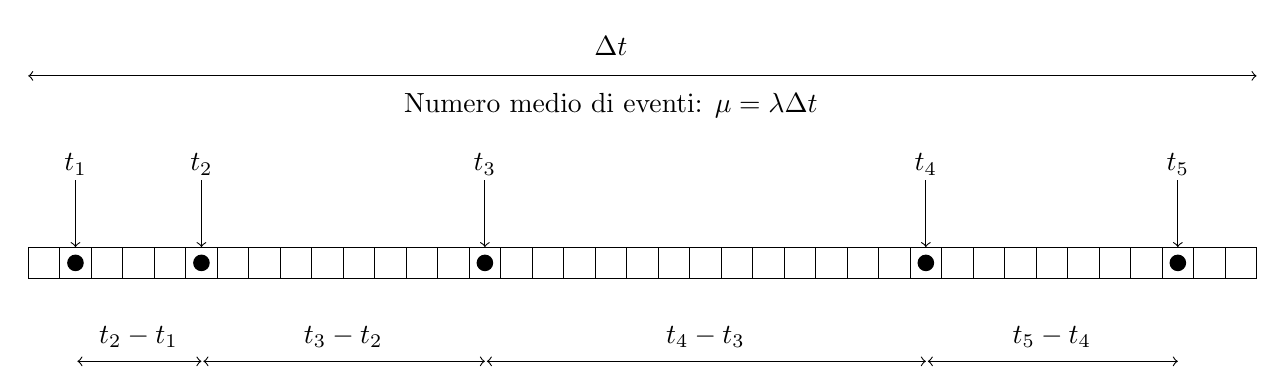
\begin{tikzpicture}[main node/.style={rectangle,draw,minimum size=4mm}]%
  \pgfmathsetmacro{\xscale}{0.4}
  \pgfmathsetmacro{\yscale}{1.25}
  \foreach \x in {1,...,39}
  \node[main node] at (\x*\xscale, 0) {};
  \foreach \e[count=\xi from 1] in {2,6,15,29,37} {
    \fill (\e*\xscale, 0) circle [radius=3pt];
    \node (e) at (\e*\xscale, \yscale) {$t_\xi$};
    \draw [out=-90,in=90,-{>[scale=1.8]}] (\e*\xscale, \yscale-0.5*\xscale) to (\e*\xscale, 0.5*\xscale);
  }
  \draw [out=0,in=180,{<[scale=1.8]}-{>[scale=1.8]}] (0.5*\xscale,1.9*\yscale) to (39.5*\xscale,1.9*\yscale);
  \node at (19*\xscale,2.2*\yscale) {$\Delta t$};
  \node at (19*\xscale,1.6*\yscale) {Numero medio di eventi: $\mu = \lambda \Delta t$};
  
  \node[inner sep=0pt] (e) at (2*\xscale, -1*\yscale) {};
  \foreach \e[count=\xi from 1] in {6,15,29,37} {
    \draw [out=0,in=180,{<[scale=1.8]}-{>[scale=1.8]}] (e) to (\e*\xscale, -1*\yscale);
    \node[inner sep=0pt] (e) at (\e*\xscale, -1*\yscale) {};
  }
  \node at (4*\xscale,-0.75*\yscale) {$t_2 - t_1$};
  \node at (10.5*\xscale,-0.75*\yscale) {$t_3 - t_2$};
  \node at (22*\xscale,-0.75*\yscale) {$t_4 - t_3$};
  \node at (33*\xscale,-0.75*\yscale) {$t_5 - t_4$};
\end{tikzpicture}

  \end{center}
  \caption{Rappresentazione schematica di un processo Poissoniano nel dominio
    del tempo con frequenza caratteristica $\lambda$
    (cfr. figura~\ref{fig:processo_poissoniano}). La distanza temporale media
    tra due eventi successivi è $\lambda^{-1}$ ma, data la natura aleatoria
    del processo, gli eventi, ovviamente, non sono equispaziati.
  }
  \label{fig:processo_poissoniano_exp}
\end{figure}

Per prima cosa $t$ è una variabile aleatoria: è ovvio che gli eventi
in un processo Poissoniano non sono temporalmente equispaziati---perché se
così fosse il numero di eventi in un intervallo di tempo fissato non
fluttuerebbe, ma sarebbe determinato a priori. Calcolare la media di $t$ non
è difficile: abbiamo in media $\mu = \lambda \Delta t$ eventi in un intervallo
di lunghezza $\Delta t$ per cui il tempo medio tra due eventi successivi
è
\begin{align*}
  \expect{t} = \frac{\Delta t}{\mu} = \frac{\Delta t}{\lambda \Delta t} =
  \frac{1}{\lambda},
\end{align*}
ovvero l'inverso della frequenza caratteristica del processo $\lambda$.
(Notiamo che $\lambda$ ha le dimensioni fisiche di $[t]^{-1}$, per cui la
nostra equazione è, come deve essere, dimensionalmente corretta. Se
$\lambda$ è $10$~s$^{-1}$, cioè $10$~Hz, allora la distanza media tra
due eventi successivi è $0.1$~s.)

Ma possiamo fare molto di più. Possiamo calcolare l'espressione esplicita per
la funzione di distribuzione di $t$ notando che, dato il fatto che un evento
si sia verificato ad un certo istante $t_0$, la probabilità (infinitesima) che
l'evento successivo si verifichi entro un intervallino (infinitesimo) di
durata $dt$ ad una distanza temporale $t$ è data dal prodotto
\begin{align*}
  dP(t, dt) = e^{-\lambda t} \times \lambda dt,
\end{align*}
in cui il primo termine rappresenta la probabilità che non si verifichi nessun
evento tra i tempi $t_0$ e $t_0 + t$ ed il secondo la probabilità che si
verifichi esattamente un evento tra i tempi $t_0 + t$ e $t_0 + t + dt$.
Dividendo entrambi i membri per $dt$ possiamo calcolare la probabilità
specifica per unità di tempo---vale a dire la nostra densità di
probabilità
\begin{align}\label{eq:distanza_eventi_poisson}
  p(t;\lambda) = \lambda e^{-\lambda t}.
\end{align}
Le distanze tra eventi successivi in un processo Poissoniano sono distribuite
esponenzialmente. Studieremo in dettaglio le proprietà
della~\eqref{eq:distanza_eventi_poisson} nella
sezione~\ref{sec:distribuzione_esponenziale}, ma anticipiamo che, come abbiamo
già detto, la media di $t$ è $\expect{t} = \lambda^{-1}$.


%\subsection{Istogrammi: statistica binomiale o Poissoniana?}
%
%Abbiamo incontrato i grafici a barre e gli istrogrammi per la prima volta nella
%sezione~\ref{sec:barre_e_istogrammi}. Questo è il momento giusto per
%tornare sull'argomento alla luce di ciò che di nuovo abbiamo imparato nel
%frattempo.


\subsection{Somma di variabili Poissoniane}

Consideriamo due variabili Poissoniane (indipendenti) $l$ ed $m$ con medie
$\mu_l$ e $\mu_m$ rispettivamente. Ci proponiamo di capire come è distribuita
la loro somma $k = l + m$. Formalmente dobbiamo sommare, per un dato valore di
$k$, su tutte le coppie di numeri positivi che danno come somma $k$; ad
esempio possiamo ottenere $k = 2$ con $l = 0$ e $m = 2$ oppure
$l = 1$ e $m = 1$ o ancora $l = 2$ e $m = 0$. In generale:
\begin{align}
  \prob{k} = \sum_{l=0}^{k} \poissonpdf[\mu_l]{l}\; \poissonpdf[\mu_m]{k-l}
\end{align}
(abbiamo utilizzato la moltiplicazione delle probabilità per eventi
indipendenti). Esplicitamente:
\begin{align*}
  \prob{k} = \sum_{l=0}^{k} \frac{\mu_l^l}{l!}e^{-\mu_l} \cdot
  \frac{\mu_m^{k-l}}{(k-l)!}e^{-\mu_m} =
  e^{-(\mu_l+\mu_m)} \sum_{l=0}^{k} \frac{\mu_l^l\mu_m^{k-l}}{l!(k-l)!} =
  \frac{e^{-(\mu_l+\mu_m)}}{k!} \sum_{l=0}^{k} \binom{k}{l} \mu_l^l\mu_m^{k-l}.
\end{align*}
Ma nella sommatoria finale riconosciamo la potenza di
binomio~\eqref{eq:potenza_binomio}, per cui:
\begin{align}
  \prob{k} = \frac{\power[k]{\mu_l+\mu_m}}{k!}e^{-(\mu_l+\mu_m)} =
  \poissonpdf[\mu_l+\mu_m]{k},
\end{align}
cioè la somma di due variabili Poissoniane è ancora una variabile
Poissoniana la cui media è la somma delle medie. (Va da sé che questo
risultato si può estendere alla somma di un numero arbitrario di variabili
Poissoniane.)

\begin{examplebox}
  \begin{example}[ma il postino viene veramente tutti i giorni?]%
    \label{example:postino_poisson}
    Supponiamo di ricevere in media $75$ lettere l'anno. Un giorno arriviamo
    a casa e troviamo nella cassetta della posta $5$ lettere (nessuna delle
    quali era presente il giorno precedente). Possiamo concludere che il
    postino non consegna la posta tutti i giorni?

    Per la discussione che segue assumeremo che la consegna della posta avvenga
    (di norma) anche la domenica e che il flusso di missive ad un certo
    indirizzo sia un fenomeno stazionario. La prima è un'assunzione
    \emph{innocua} (che facciamo solo per evitare complicazioni inessenziali),
    mentre la seconda è un'assunzione \emph{forte}---ma non del tutto
    irragionevole, o almeno non così irragionevole da rendere la
    discussione irrilevante.
    Sotto queste ipotesi il numero $k$ di lettere che, giorno per giorno,
    troviamo nella cassetta della posta è una variabile Poissoniana, la cui
    media può essere stimata come $m = 75/365 \approx 0.2$. Possiamo allora
    riformulare in termini quantitativi la domanda iniziale chiedendoci
    quale sia  la probabilità di trovare $5$ o più lettere quando in media
    ce ne attendiamo $0.2$:
    \begin{align*}
      \prob{k \geq 5} = \sum_{k=5}^{\infty} \poissonpdf[m]{k}.
    \end{align*}
    Si tratta del tipico caso in cui il teorema della probabilità totale
    permette di aggirare la serie infinita:
    \begin{align*}
      \prob{k \geq 5} = 1 - \prob{k < 5} = 1 - \sum_{k=0}^{4} \poissonpdf[m]{k} =
      1 - \sum_{k=0}^{4} \frac{m^k}{k!}e^{-m} \approx 2.6 \times 10^{-6}.
    \end{align*}
    La probabilità è abbastanza piccola (almeno sotto le ipotesi iniziali)
    da legittimarci ad un reclamo ufficiale.

    Chiediamoci adesso quale sia la probabilità di trovare nella cassetta
    della posta $5$ lettere nell'ipotesi in cui il postino consegni la
    corrispondenza solo una volta alla settimana.
    La somma di $7$ variabili Poissoniane con media $m$ è una variabile
    Poissoniana con media $m_s = 7m = 525/365 \approx 1.44$, e adesso:
    \begin{align*}
      \prob{k \geq 5} = 1 - \prob{k < 5} =
      1 - \sum_{k=0}^{4} \poissonpdf[m_s]{k} =
      \sum_{k=0}^{4} \frac{m_s^k}{k!}e^{-m_s} \approx 1.6\%,
    \end{align*}
    che è piccola ma decisamente non piccola come prima.
  \end{example}
\end{examplebox}



%\subsection{La distribuzione di Poisson composta}


\section{La distribuzione uniforme}
\label{sec:distribuzione_uniforme}

La distribuzione uniforme è l'esempio più semplice di funzione di
distribuzione di variabile casuale continua---la densità di probabilità
è costante entro un intervallo finito e nulla fuori:
\begin{align}\label{eq:uniform_pdf}
  \uniformpdf[a, b]{x} = \left \{ \begin{array}{ll}
    \frac{\displaystyle 1}{\displaystyle (b - a)} & a \leq x \leq b\\
    0 & x < a ; ~ x > b
  \end{array} \right.
\end{align}
Un esempio particolare della densità di probabilità per una distribuzione
uniforme (con $a = 0$ e $b = 1$) è mostrato in figura~\ref{fig:pdf_uniforme}.

\pgffigone{pdf_uniforme}{
  Esempio di distribuzione uniforme per $a = 0$ e $b = 1$.
}


\subsection{Normalizzazione, media, varianza e coefficiente di asimmetria}

Si dimostra banalmente che la distribuzione, così come è scritta
nella~\eqref{eq:uniform_pdf}, è correttamente normalizzata:
\begin{align*}
  \intinf \uniformpdf[a,b]{x} \diff =
  \int_a^b \frac{1}{(b - a)} \diff =
  \frac{1}{(b - a)} \int_a^b \diff =
  \frac{1}{(b - a)}\, (b - a) = 1
\end{align*}
(Abbiamo calcolato esplicitamente l'integrale, ma di fatto si tratta
semplicemente dell'area di un rettangolo di base $(b - a)$ e di altezza
$\nicefrac{1}{(b - a)}$---$1$, appunto.)

La media è data, per definizione, dal valore di aspettazione della
variabile casuale
\begin{align}\label{eq:media_uniforme}
  \mu = \expect{x} = \intinf x \uniformpdf[a,b]{x} \diff =
  \frac{1}{(b - a)} \int_a^b x \diff =
  \frac{1}{(b - a)} \eval{\frac{x^2}{2}}{a}{b} =
  \frac{1}{(b - a)} \, \frac{(b^2 - a^2)}{2} = \frac{(b + a)}{2}
\end{align}
e coincide con il valor medio dell'intervallo su cui la densità di
probabilità è non nulla---il che non dovrebbe sorprendere perché la
funzione di distribuzione è simmetrica rispetto all'asse
$x = \nicefrac{(b + a)}{2}$. Per lo stesso motivo la mediana coincide con la
media, mentre la moda non è definita poiché la densità di probabilità
non ha un massimo.

Procediamo con il calcolo della varianza. Al solito partiamo
dalla~\eqref{eq:variance_alt} e calcoliamo prima il valore di aspettazione di
$x^2$:
\begin{align*}
  \expect{x^2} & =
  \intinf x^2 \uniformpdf[a,b]{x} \diff =
  \frac{1}{(b - a)} \int_a^b x^2 \diff =
  \frac{1}{(b - a)} \eval{\frac{x^3}{3}}{a}{b} =
  \frac{1}{(b - a)} \, \frac{(b^3 - a^3)}{3} = \\
  & = \frac{1}{(b - a)} \, \frac{(b-a)(b^2 + ab + a^2)}{3} =
  \frac{(b^2 + ab + a^2)}{3}
\end{align*}
da cui
\begin{align}\label{eq:varianza_uniforme}
  \sigma^2 & = \expect{x^2} - \mu^2 =
  \frac{(b^2 + ab + a^2)}{3} -\frac{(b + a)^2}{4} =
  \frac{(4b^2 + 4ab + 4a^2 - 3b^2 -6ab - 3 a^2)}{12} = \nonumber\\
  & = \frac{(b^2 - 2ab + a^2)}{12} = \frac{(b - a)^2}{12}
\end{align}
e
\begin{align}\label{eq:stdev_uniforme}
  \sigma = \frac{(b - a)}{\sqrt{12}}.
\end{align}
Questa $\sqrt{12}$ al denominatore della deviazione standard è un numero
importante da tenere a memoria, perché è quello che determina l'incertezza
di misura (nel senso statistico) di tutti gli strumenti digitali---cioè
di quegli strumenti che forniscono in uscita valori discreti (spaziati tra
di loro di una quantità pari alla risoluzione strumentale) non affetti da
fluttuazioni statistiche.

Per completezza la semilarghezza a metà altezza è pari alla semilarghezza
dell'intervallo su cui la densità di probabilità è non nulla:
\begin{align}
  \hwhm = \frac{(b - a)}{2} = \sqrt{3} \sigma \approx 1.73 \sigma.
\end{align}

Poiché la distribuzione è simmetrica rispetto al valor medio, il
coefficiente di asimmetria $\skewness$---e, più in generale, tutti i
momenti centrali di ordine dispari---è banalmente nullo.


\begin{examplebox}
  \begin{example}
    Supponiamo di misurare la massa di un oggetto con una bilancia digitale con
    la risoluzione di un grammo; sia $m = 58$~g il valore indicato
    dal display. Se possiamo escludere la presenza di effetti sistematici è
    ragionevole ammettere che il misurando sia compreso, con densità di
    probabilità uniforme, tra $57.5$ e $58.5$~g. La media della distribuzione
    sarà $58$~g e la deviazione standard $\nicefrac{1}{\sqrt{12}} = 0.289$~g.
    Se vogliamo attribuire un errore statisticamente corretto alla nostra misura
    scriveremo, al livello di una deviazione standard:
    \begin{align*}
      m = 58.0 \pm 0.3~\text{g}
    \end{align*}
  \end{example}
\end{examplebox}


\subsection{Funzione cumulativa e quantili}

La funzione cumulativa della distribuzione uniforme si calcola banalmente come
\begin{align}
  F(x) = \int_a^x \frac{1}{(b - a)} \diff[t] = \frac{(x - a)}{b - a}
  \quad a \leq x \leq b,
\end{align}
da cui la funzione di distribuzione inversa è
\begin{align}
  F^{-1}(q) = q(b - a) + a.
\end{align}


\section{La distribuzione esponenziale}
\label{sec:distribuzione_esponenziale}

Abbiamo già incontrato la distribuzione esponenziale nella
sezione~\ref{sec:distanza_eventi_poisson}, a proposito della distanza tra
due eventi successivi in un processo
Poissoniano~\eqref{eq:distanza_eventi_poisson}. In generale, dato un numero
positivo $\lambda > 0$ una distribuzione della forma
\begin{align}\label{eq:exponential_pdf}
  \exponentialpdf[\lambda]{x} = \left \{ \begin{array}{ll}
    \lambda e^{-\lambda x} & 0 \leq x \leq \infty\\
    0 & x < 0
  \end{array} \right.
\end{align}
si dice esponenziale con parametro $\lambda$. Vedremo tra un attimo che
$\lambda$ (che per ragioni dimensionali ha le dimensioni di $x^{-1}$) ha il
significato fisico dell'inverso della media della distribuzione, per cui
a volte la~\eqref{eq:exponential_pdf} si trova anche scritta in funzione
di $\lambda^{-1}$---che prende il nome di \emph{vita media} nel caso di processi
Poissoniani nel dominio del tempo e \emph{cammino libero medio} nel caso di
processi Poissoniani nel dominio dello spazio. Due esempi di distribuzione
esponenziale, per due diversi valori di $\lambda$, sono mostrati in
figura~\ref{fig:pdf_esponenziale_1_pdf_esponenziale_2}.

\pgffigtwo{pdf_esponenziale_1}{pdf_esponenziale_2}{
  Esempi di distribuzione esponenziale~\eqref{eq:exponential_pdf} per
  due diversi valori di $\lambda$ ($1$ e $2$). Entrambe le distribuzioni
  sono correttamente normalizzate.
}


\subsection{Normalizzazione, media, varianza e coefficiente di asimmetria}

La distribuzione esponenziale, così come scritta
nella~\eqref{eq:exponential_pdf}, è correttamente normalizzata:
\begin{align*}
\int_0^\infty \exponentialpdf[\lambda]{x} \diff =
\int_0^\infty \lambda e^{-\lambda x} \diff =
\eval{-e^{-\lambda x}}{0}{\infty} = 1.
\end{align*}

La media della distribuzione si calcola al solito secondo la
definizione~\ref{eq:mean} e vale
\begin{align}
  \mu & = \expect{x} =
  \int_{-\infty}^\infty x \exponentialpdf[\lambda]{x} \diff =
  \int_0^\infty x \lambda e^{-\lambda x} \diff =
  \frac{1}{\lambda} \int_0^\infty r e^{-r}\diff[r] =
  \frac{1}{\lambda} \left(
  \eval{-r e^{-r}}{0}{\infty} \;\;\; +
  \int_0^\infty e^{-r}\diff[r]
  \right) = \nonumber\\
  & = \eval{-\frac{1}{\lambda}e^{-r}}{0}{\infty} \;\;\; = \frac{1}{\lambda}.
\end{align}
(in cui abbiamo operato il cambiamento di variabile $\lambda x = r$, ed
abbiamo calcolato l'integrale risultante per parti).

Per la varianza, al solito, si parte dal valore di aspettazione di $x^2$,
che si calcola con lo stesso cambiamento di variabile $\lambda x = r$ ed
integrando per parti due volte
\begin{align*}
  \expect{x^2} =
  \int_0^\infty x^2 \exponentialpdf[\lambda]{x} \diff =
  \int_0^\infty x^2 \lambda e^{-\lambda x} \diff =
  \frac{1}{\lambda^2} \int_0^\infty r^2 e^{-r}\diff[r] =
  \frac{1}{\lambda^2}\left(
  \eval{-r^2 e^{-r}}{0}{\infty} +
  2\int_0^\infty t e^{-t}\diff[t]
  \right) = \frac{2}{\lambda^2}.
\end{align*}
Si ha dunque
\begin{align}
  \sigma^2 = \expect{x^2} - \mu^2 = \frac{2}{\lambda^2} - \frac{1}{\lambda^2} =
  \frac{1}{\lambda^2}
\end{align}
e
\begin{align}
  \sigma = \frac{1}{\lambda}.
\end{align}

La distribuzione esponenziale vale $\lambda$ per $x = 0$ e la retta orizzontale
$y = \nicefrac{\lambda}{2}$ interseca la funzione densità di probabilità
in $x = 0$ ed in corrispondenza della radice dell'equazione
\begin{align*}
  \frac{\lambda}{2} = \lambda e^{-\lambda x} \quad \text{ovvero} \quad
  x = \frac{\ln 2}{\lambda}.
\end{align*}
Ne deriva immediatamente che la semilarghezza a metà altezza è data da
\begin{align}
  \hwhm = \frac{\ln 2}{2\lambda} = \frac{\ln 2}{2}\sigma \approx 0.347\sigma.
\end{align}

Integrando per parti come abbiamo fatto per il calcolo della media e della
varianza è semplice ricavare per ricorrenza i momenti algebrici di
ordine superiore
\begin{align*}
  \expect{x^n} = \int_0^\infty x^n \lambda e^{-\lambda x}\diff =
  \eval{- x^n e^{-\lambda x}}{0}{\infty} \:\: +
  \frac{n}{\lambda} \int_0^\infty x^{n-1} \lambda e^{-\lambda x}\diff =
  \frac{n}{\lambda}\expect{x^{n-1}}.
\end{align*}
Il momento algebrico di ordine $3$, ad esempio, vale
\begin{align*}
  \expect{x^3} = \frac{3}{\lambda}\expect{x^2} = \frac{6}{\lambda^3},
\end{align*}
da cui
\begin{align}
  \momcen{3} = \expect{x^3} - 3\mu\sigma^2 - \mu^3 = \frac{2}{\lambda^3}
  \quad \text{e} \quad
  \skewness = 2.
\end{align}
(Che il coefficiente di asimmetria sia sempre positivo è cosa che non dovrebbe
stupire perché la distribuzione ha una coda pronunciata per valori di $x$
a destra delle media.)


\subsection{Funzione cumulativa e quantili}

La funzione cumulativa della distribuzione esponenziale ha una espressione
analitica semplice
\begin{align}
  F(x) = \int_0^{x} \lambda e^{-\lambda t} \diff[t] =
  \eval{-e^{-\lambda t}}{0}{x} \:\: =
  1 - e^{-\lambda x},
\end{align}
che altrettanto semplicemente si può invertire per ricavare la funzione di
distribuzione inversa
\begin{align}
  F^{-1}(q) = -\frac{\ln(1 - q)}{\lambda}.
\end{align}
la funzione cumulativa e la funzione di distribuzione inversa sono mostrate
in figura~\ref{fig:cdf_esponenziale_ppf_esponenziale} per una distribuzione
esponenziale con parametro $\lambda = 1$.

\pgffigtwo{cdf_esponenziale}{ppf_esponenziale}{
  Funzione cumulativa e funzione di distribuzione inversa per una distribuzione
  esponenziale con parametro $\lambda = 1$.
}


\subsection{Assenza di memoria}

Una proprietà interessante della distribuzione esponenziale è costituita
dal fatto che
\begin{align*}
  \prob{x \geq x_1 + x_2} =
  \int_{x_1 + x_2}^\infty\!\!\!\!\!\!\exponentialpdf[\lambda]{x}\diff =
  \lambda \int_{x_1 + x_2}^\infty\!\!\!\!\!\!e^{-\lambda x}\diff =
  e^{-\lambda (x_1 + x_2)},
\end{align*}
da cui segue banalmente che
\begin{align}\label{eq:esponenziale_cumul_compl}
  \prob{x \geq x_1 + x_2} = \prob{x \geq x_1}\prob{x \geq x_2}.
\end{align}
Ora, per definizione di probabilità condizionata, si ha anche che
\begin{align*}
  \prob{x \geq x_1 + x_2} =
  \prob{x \geq x_1 + x_2 \cond x \geq x_1}\prob{x \geq x_1},
\end{align*}
per cui la~\eqref{eq:esponenziale_cumul_compl} si può anche scrivere come
\begin{align}\label{eq:esponenziale_assenza_memoria}
  \prob{x \geq x_1 + x_2 | \, x \geq x_1} = \prob{x \geq x_2}.
\end{align}
Una variabile casuale che goda di questa proprietà si dice una variabile
\emph{senza memoria} (o anche \foreign{memory-less}).


\begin{examplebox}
  \begin{example}
    Supponiamo che il cammino libero medio $l_0$ di una particella in un
    certo mezzo (omogeneo) sia $1$~mm. Quando la particella penetra nel mezzo,
    in generale percorrerà una certa distanza $x$ (che, a parità di
    condizioni iniziali, varia in modo casuale di volta in volta) prima di
    interagire; come detto prima, questa distanza è descritta da una
    densità di probabilità di tipo esponenziale con parametro
    $\lambda = \nicefrac{1}{l_0}$:
    \begin{align*}
      p(x) = \frac{1}{l_0}e^{-\frac{x}{l_0}}.
    \end{align*}
    Il valore di aspettazione della variabile $x$ è $l_0$. Il che
    significa, in altre parole, che la nostra particella percorre in media
    una distanza $l_0$ prima di interagire (da cui il nome di cammino
    libero medio). Ci chiediamo quale sia la probabilità che la particella
    percorra un distanza $l = 10l_0$ prima di interagire.

    La risposta è, banalmente
    \begin{align*}
      \prob{x \geq 10l_0} = e^{-10} \approx 4.54 \times 10^{-5},
    \end{align*}
    cioè è estremamente poco probabile che una particella percorra una
    distanza maggiore a 10 volte il cammino libero medio prima di interagire.
  \end{example}

  \begin{example}
    Supponiamo di {\itshape osservare}, a partire da un istante $t_0$, un
    nucleo radioattivo con vita media (inverso del parametro $\lambda$) di
    $1$~s. La probabilità che, dopo un secondo, il nucleo non sia decaduto
    è:
    \begin{align*}
      \prob{x \geq 1} = e^{-1} \approx 37\%
    \end{align*}
    Supponiamo adesso che il nucleo non sia ancora decaduto dopo $10$~s, il che
    è estremamente improbabile ma possibile (a proposito: quanto vale la
    probabilità di questo evento?). Ebbene: la probabilità che il nucleo
    non decada tra $t_0 + 10$~s e $t_0 + 11$~s è di nuovo il $37\%$.

    Tanto per fissare le idee: se la stessa cosa valesse per un'automobile,
    ad ogni istante una vettura appena uscita dal concessionario ed una con
    $200000$~km alle spalle avrebbero la stessa probabilità di rompersi
    entro il giorno successivo. Purtroppo, al contrario dei nuclei
    radioattivi le auto hanno memoria della propria storia!
  \end{example}
\end{examplebox}


\section{La distribuzione di Gauss}
\label{sec:distribuzione_gauss}

\foreign{"Everyone believes in it: experimentalists believing that it is a
  mathematical theorem, mathematicians believing that it is an empirical
  fact."}
Questa osservazione, generalmente attribuita a Henri Poincaré, riassume
efficacemente la rilevanza che la più \emph{celebre} funzione di
distribuzione---quella di Gauss, appunto---riveste nella teoria della
probabilità e nella statistica. Come vedremo nel seguito, la distribuzione di
Gauss può essere vista come il limite di una distribuzione di Poisson per
$\mu \rightarrow \infty$ o di una distribuzione binomiale nel limite
$n \rightarrow \infty$ (questa volta senza nessuna ipotesi aggiuntiva su $p$).
Inoltre, per il teorema centrale del limite, la distribuzione della media di
un numero abbastanza grande di campionamenti di una variabile casuale,
indipendentemente dalla sua distribuzione, è distribuita Gaussianamente.
Questi sono solo alcuni dei motivi per cui questa distribuzione si trova
così spesso in pratica.


\subsection{La distribuzione di Gauss come limite della Poissoniana}
\label{sec:gauss_limite_poisson}

Consideriamo una variabile casuale Poissoniana $k$ e calcoliamo il
logaritmo naturale della sua funzione di distribuzione
\begin{align*}
  \ln\poissonpdf[\mu]{k} = \ln\left( \frac{\mu^k}{k!}\,e^{-\mu} \right) =
  k\ln\mu -\ln(k!) - \mu.
\end{align*}
Il termine più problematico è chiaramente quello con il fattoriale, ma
se $\mu$ è molto grande (e quindi anche $k$ è tendenzialmente molto grande,
visto che $\mu = \expect{k}$) possiamo utilizzare la formula di
Stirling~\eqref{eq:formula_di_stirling_log} e riscrivere la nostra espressione
(questa volta in forma approssimata) come
\begin{align*}
  \ln\poissonpdf[\mu]{k} \approx
  k\ln\mu - \frac{1}{2}\ln(2\pi k) - k\ln k + k - \mu.
\end{align*}
L'idea è adesso quella di sviluppare in qualche modo questa espressione in
serie di Taylor, ma il problema di fondo è lo stesso che abbiamo incontrato
nel derivare la distribuzione di Poisson come limite della binomiale: possiamo
fare il limite per $\mu \rightarrow \infty$, ma allo stesso tempo abbiamo
bisogno di una prescrizione per $k$, che è una variabile casuale e, come tale,
non è univocamente determinata da $\mu$. Introduciamo dunque la variabile
casuale \emph{ridotta}
\begin{align*}
  \delta = \frac{k - \mu}{\mu} \quad \text{ovvero} \quad k = \mu(1 + \delta).
\end{align*}
Le fluttuazioni di $k$ attorno al valor medio (e quindi il valore del
numeratore dell'espressione appena scritta) saranno dell'ordine di
$\sigma = \sqrt{\mu}$ e, per $\mu \rightarrow \infty$, $\delta \rightarrow 0$
come $\nicefrac{1}{\sqrt{\mu}}$. Possiamo dunque scrivere
\begin{align*}
  \ln\poissonpdf[\mu]{\delta} \approx
  \mu(1 + \delta)\ln\mu - \frac{1}{2}\ln\left(2\pi \mu(1 + \delta)\right) -
  \mu(1 + \delta)\ln\left(\mu(1 + \delta)\right) + \mu(1 + \delta) - \mu.
\end{align*}
A questo punto possiamo sviluppare in serie attorno al valore $\delta = 0$---e
vedremo tra un secondo che sviluppare al prim'ordine non basta ed avremo
bisogno del termine con la derivata seconda. Il calcolo è un po' tedioso, ma
le derivate rilevanti sono
\begin{align*}
  \td{\ln\poissonpdf[\mu]{0}}{\delta}{} & =
  \at{- \mu \ln(1 + \delta) - \frac{1}{2(1 + \delta)}}{\delta = 0} =
  -\frac{1}{2} \quad \text{e} \quad
  \td[2]{\ln\poissonpdf[\mu]{0}}{\delta}{} & =
  \at{-\frac{\mu}{(1 + \delta)} + \frac{1}{2(1 + \delta)^2}}{\delta = 0} =
  -\mu + \frac{1}{2},
\end{align*}
da cui
\begin{align*}
  \ln\poissonpdf[\mu]{\delta} \approx \ln\poissonpdf[\mu]{0} +
  \td{\ln\poissonpdf[\mu]{0}}{\delta}{} \delta +
  \frac{1}{2}\td[2]{\ln\poissonpdf[\mu]{0}}{\delta}{}
  \delta^2 = -\frac{1}{2}\ln\left(2\pi \mu\right) - \frac{1}{2}\delta -
  \frac{1}{2}\mu\delta^2 + \frac{1}{4} \delta^2.
\end{align*}
Guardiamo più attentamente la relazione che abbiamo appena ottenuto. Per
$\delta \rightarrow 0$ il secondo ed il quarto termine si annullano (che è il
motivo per cui non abbiamo troncato lo sviluppo al prim'ordine) ed il terzo è
quello rilevante---nel valutare la forma indeterminata $\mu\delta^2$ ricordiamo
che $\delta \rightarrow 0$ come $\nicefrac{1}{\sqrt{\mu}}$. Possiamo adesso
ripristinare il $k$ che avevamo momentaneamente \emph{nascosto}, col che
otteniamo
\begin{align}\label{eq:poisson_gauss}
  \ln\poissonpdf[\mu]{k} \approx
  -\frac{1}{2}\ln\left(2\pi \mu\right) - \frac{1}{2}\frac{(k - \mu)^2}{\mu}
  \quad \text{ovvero} \quad
  \poissonpdf[\mu]{k} \approx
  \frac{1}{\sqrt{2\pi\mu}}\,e^{-\frac{1}{2}\frac{(k - \mu)^2}{\mu}}.
\end{align}

\begin{table}[!hbt]
  \tablehstack{
    \begin{tabular}{lrrr}%
      \hline
      $k$ & $\poissonpdf[100]{k}$ & Equazione~\eqref{eq:poisson_gauss}
      & Errore relativo\\
      \hline
      \hline
      %$80$&$5.198\times 10^{-3}$&$5.399\times 10^{-3}$&$3.87\times 10^{-2}$\\
      %$85$&$1.321\times 10^{-2}$&$1.295\times 10^{-2}$&$1.92\times 10^{-2}$\\
      $90$&$2.504\times 10^{-2}$&$2.420\times 10^{-2}$&$3.36\times 10^{-2}$\\
      $95$&$3.601\times 10^{-2}$&$3.521\times 10^{-2}$&$2.24\times 10^{-2}$\\
      $100$&$3.986\times 10^{-2}$&$3.989\times 10^{-2}$&$8.34\times 10^{-4}$\\
      $105$&$3.440\times 10^{-2}$&$3.521\times 10^{-2}$&$2.34\times 10^{-2}$\\
      $110$&$2.342\times 10^{-2}$&$2.420\times 10^{-2}$&$3.31\times 10^{-2}$\\
      $115$&$1.272\times 10^{-2}$&$1.295\times 10^{-2}$&$1.84\times 10^{-2}$\\
      %$120$&$5.561\times 10^{-3}$&$5.399\times 10^{-3}$&$2.91\times 10^{-2}$\\
      \hline
    \end{tabular}
  }{
    \caption{Illustrazione della validità della~\eqref{eq:poisson_gauss} come
      approssimazione della distribuzione di Poisson, per alcuni valori
      rappresentativi di $k$ e $\mu = 100$. L'errore relativo è di qualche
      \% al massimo, e l'approssimazione migliora al crescere di $\mu$.}
    \label{tab:poisson_gauss}
  }
\end{table}

\pgffigtwo{poisson_gauss1}{poisson_gauss2}{
  Approssimazione Gaussiana della distribuzione di Poisson per due diversi
  valori della media---$\mu = 5$ e $\mu = 100$.
}


A questo livello la~\eqref{eq:poisson_gauss} è un'espressione approssimata per
la~\eqref{eq:poisson_pdf} che può essere utilizzata quando $\mu$ è grande,
come illustrato in figura~\ref{fig:poisson_gauss1_poisson_gauss2} ed in
tabella~\ref{tab:poisson_gauss}. Ma fermiamoci per un attimo ad osservare meglio
la relazione che abbiamo appena ricavato.
Per prima cosa la~\eqref{eq:poisson_gauss} è simmetrica rispetto al valor
medio della distribuzione $k =\mu$. Questo non dovrebbe sorprendere, poiché
sappiamo già che il coefficiente di asimmetria della distribuzione di Poisson
vale $\skewness = \nicefrac{1}{\sqrt{\mu}}$, che tende a $0$ per
$\mu \rightarrow \infty$. (In altre parole sapevamo già
dalla~\eqref{eq:poisson_asimmetria} che la distribuzione di Poisson tende a
diventare simmetrica per valori grandi della media.) La seconda osservazione è
che, dato che la varianza $\sigma^2$ della distribuzione di Poisson è uguale
al valor medio $\mu$, possiamo in effetti riscrivere la~\eqref{eq:poisson_gauss}
nella forma alternativa
\begin{align*}
  \poissonpdf[\mu]{k} \approx
  \frac{1}{\sigma\sqrt{2\pi}}\,e^{-\frac{1}{2}\left(\frac{k - \mu}{\sigma}\right)^2}.
\end{align*}

Se adesso sostituiamo la variabile casuale discreta $k$ con una variabile
continua $x$, e lasciamo la deviazione standard $\sigma$ libera di variare
indipendentemente dalla media, abbiamo ottenuto la distribuzione di Gauss che
studieremo in dettaglio nelle prossime sottosezioni. Torneremo più in
dettaglio sul passaggio dal discreto al continuo nel seguito.


\subsection{Normalizzazione, media e varianza}

La funzione di distribuzione di Gauss (o distribuzione normale) si scrive dunque
nella forma
\begin{equation}\label{eq:gauss_pdf}
  \gausspdf[\mu, \sigma]{x} =
  \frac{1}{\sigma\sqrt{2\pi}} \, e^{-\frac{1}{2}\left(\frac{x-\mu}{\sigma}\right)^2}
\end{equation}
dove $\mu$ e $\sigma^2$, come vedremo tra un attimo, sono proprio la media e
la varianza della distribuzione nel senso delle~\eqref{eq:mean}
e~\eqref{eq:variance}---e sono indipendenti tra di loro (cioè non sono più
necessariamente coincidenti come nel caso Poissoniano). Una variabile casuale
Gaussiana $z$ con media $0$ e varianza $1$, che ha funzione di distribuzione
(completamente fissata)
\begin{equation}\label{eq:gauss_pdf_std}
  \gausspdf{z} = \frac{1}{\sqrt{2\pi}} \, e^{-\frac{1}{2}z^2},
\end{equation}
si dice variabile Gaussiana \emph{in forma standard}. Una variabile Gaussiana
generica $x$ può essere trasformata nella corrispondente variabile in forma
standard attraverso il cambio di variabile
\begin{align}\label{eq:gauss_variabile_standard}
  z = \frac{x - \mu}{\sigma} \quad \text{ovvero} \quad
  x = \sigma z + \mu.
\end{align}
Si tratta di una trasformazione importante, che utilizzeremo spesso nel seguito,
e, per completezza, verifichiamo esplicitamente che tutto funzioni come deve:
\begin{align*}
  \expect{z} = \expect{\frac{x - \mu}{\sigma}} =
  \frac{1}{\sigma}\left(\expect{x} - \expect{\mu}\right) = 0
  \quad \text{e} \quad
  \var{z} = \expect{z^2} = \expect{\frac{(x - \mu)^2}{\sigma^2}} =
  \frac{1}{\sigma^2}\expect{(x - \mu)^2} = 1.
\end{align*}

\pgffigtwo{pdf_gauss_1}{pdf_gauss_2}{
  Esempi di distribuzione di Gauss~\eqref{eq:gauss_pdf} per $\mu = 0$
  e due diversi valori di $\sigma$ ($1$ e $2$). Si noti che l'altezza della
  distribuzione (cioè il valore in $x = 0$) è inversamente proporzionale
  alla deviazione standard, per cui essa dimezza quando $\sigma$ raddoppia.
}

La distribuzione di Gauss è mostrata in
figura~\ref{fig:pdf_gauss_1_pdf_gauss_2} per due valori diversi di $\sigma$.
Notiamo esplicitamente che il valore massimo della funzione (che si ha per
$x = \mu$) è inversamente proporzionale a $\sigma$, per cui se raddoppiamo
la deviazione standard della distribuzione, stiamo effettivamente
raddoppiando la larghezza e dimezzando l'altezza. (L'integrale sotto la curva
rimane costante per la condizione di normalizzazione.)

Verifichiamo che la distribuzione di Gauss, scritta nella
forma~\eqref{eq:gauss_pdf}, è correttamente normalizzata, e che---come
accennato poco fa---$\mu$ e $\sigma$ rappresentano la media e la deviazione
standard della distribuzione. Scriviamo, al solito
\begin{align*}
  \int_{-\infty}^\infty \gausspdf[\mu, \sigma]{x} \diff =
  \int_{-\infty}^\infty \frac{1}{\sigma\sqrt{2\pi}} \,
  e^{-\frac{1}{2}\left(\frac{x-\mu}{\sigma}\right)^2} \diff =
  \frac{1}{\sqrt{2\pi}}\int_{-\infty}^\infty e^{-\frac{1}{2}z^2} \diff[z] :=
  \frac{1}{\sqrt{2\pi}}\,I_0.
\end{align*}
Sfortunatamente questo integrale non ha espressione analitica, nel senso che non
esiste una primitiva dell'integrando esprimibile in forma chiusa in termini di
funzioni elementari%
\footnote{La questione è, almeno in parte, semantica, poiché l'integrale
  definito di $e^{-\frac{1}{2}z^2}$ tra due estremi arbitrari può essere
  calcolato numericamente (e tabulato, come vedremo) con il grado di accuratezza
  desiderato.}.
Un modo semplice per calcolare l'integrale definito $I_0$ è quello di
scrivere il suo quadrato come prodotto di due integrali indipendenti, utilizzare
il teorema di Fubini e passare in coordinate polari (facendo attenzione a come
trasforma l'elemento di superficie $dxdy \rightarrow rdrd\phi$)
\begin{align*}
  I_0^2 & =
  \left(\int_{-\infty}^\infty e^{-\frac{1}{2}x^2} \diff[x]\right) \times
  \left(\int_{-\infty}^\infty e^{-\frac{1}{2}y^2} \diff[y]\right) =
  \int_{-\infty}^\infty\int_{-\infty}^\infty e^{-\frac{1}{2}(x^2 + y^2)} \diff[x]\diff[y] =
  \int_0^{2\pi}\int_0^\infty e^{-\frac{1}{2}r^2}r\diff[r]\diff[\phi] =\\
  & = 2\pi \int_0^\infty e^{-\frac{1}{2}r^2} \diff[\left(\frac{r^2}{2}\right)] =
  -2\pi \eval{e^{-\frac{1}{2}r^2}}{0}{\infty} \;\;\;\; = 2\pi
  \quad \text{da cui} \quad
  I_0 = \sqrt{2\pi},
\end{align*}
che dimostra effettivamente che la distribuzione di partenza è correttamente
normalizzata.

Prima di andare avanti vale la pena spendere un istante su una classe di
integrali definiti (di cui il precedente è un caso particolare) che ci sarà
utile nel seguito, ovvero
\begin{align*}
  I_n = \int_{-\infty}^\infty x^n e^{-\frac{1}{2}x^2} \diff[x] =
  - \int_{-\infty}^\infty x^{n-1} \diff[\left(e^{-\frac{1}{2}x^2}\right)] =
  - \eval{x^{n-1} e^{-\frac{1}{2}x^2}}{-\infty}{\infty}\;\;\;\; +
  (n - 1) \int_{-\infty}^\infty x^{n-2} e^{-\frac{1}{2}x^2} \diff[x].
\end{align*}
Per ragioni di simmetria $I_n$ è nullo per $n$ dispari (l'integrando è
dispari ed il dominio, sia pure infinito, è simmetrico rispetto allo zero).
Per $n$ pari, integrando per parti, si ottiene come abbiamo appena visto
l'interessante relazione per ricorrenza
\begin{align}\label{eq:gauss_momenti}
  \begin{cases}
    I_0 & = \sqrt{2\pi}\\
    I_1 & = 0\\
    I_n & = (n - 1)\, I_{n - 2},
  \end{cases}
\end{align}
da cui $I_2 = \sqrt{2\pi}$, $I_3 = 0$, $I_4 = 3\sqrt{2\pi}$ e così via.

La media della distribuzione, formalmente, si può allora scrivere, operando
lo stesso cambiamento di variabile di prima, come
\begin{align*}
  \expect{x} = \int_{-\infty}^\infty \frac{1}{\sigma\sqrt{2\pi}}
  x e^{-\frac{1}{2}\left(\frac{x-\mu}{\sigma}\right)^2} \diff =
  \frac{1}{\sqrt{2\pi}}\int_{-\infty}^\infty
  (\sigma z + \mu) e^{-\frac{1}{2}z^2} \diff[z] =
  \frac{1}{\sqrt{2\pi}} \, (\sigma I_1 + \mu I_0) = \mu,
\end{align*}
cosa che sapevamo già poiché la distribuzione è simmetrica rispetto al
punto $x = \mu$. (Di più: questo implica anche che la mediana e la moda
coincidono e valgono anch'esse $\mu$.) La varianza sarà, come anticipato
\begin{align*}
  \expect{(x - \mu)^2} = \int_{-\infty}^\infty \frac{1}{\sigma\sqrt{2\pi}}
  (x - \mu)^2 e^{-\frac{1}{2}\left(\frac{x-\mu}{\sigma}\right)^2} \diff =
  \frac{1}{\sqrt{2\pi}}\int_{-\infty}^\infty \sigma^2z^2e^{-\frac{1}{2}z^2} \diff[z] =
  \frac{1}{\sqrt{2\pi}} \, \sigma^2 I_2 = \sigma^2.
\end{align*}
A questo punto la~\eqref{eq:gauss_momenti} ci permette di calcolare banalmente
tutti i momenti centrali di ordine superiore, ma dal nostro punto di vista
questo non è terribilmente interessante in quanto il coefficiente di
asimmetria $\skewness$ si annulla per ragioni di simmetria ed i momenti
centrali di ordine pari non ci dicono molto altro sulla distribuzione.

\`E invece interessante, come abbiamo fatto con tutte le distribuzioni
incontrate sino ad ora, calcolare il coefficiente di proporzionalità tra la
semilarghezza a metà altezza e la deviazione standard---il che si fa
risolvendo l'equazione
\begin{align*}
  \frac{1}{2} \frac{1}{\sigma\sqrt{2\pi}} =
  \frac{1}{\sigma\sqrt{2\pi}} \, e^{-\frac{1}{2}\left(\frac{x-\mu}{\sigma}\right)^2}
  \quad \text{da cui} \quad
  \frac{1}{2}\left(\frac{x-\mu}{\sigma}\right)^2 = \ln 2
  \quad \text{e} \quad
  x = \mu \pm \sqrt{2\ln 2} \, \sigma.
\end{align*}
Il valore della semilarghezza a metà altezza è dunque
\begin{align}
  \hwhm = \sqrt{2\ln 2}\, \sigma \approx 1.178 \sigma.
\end{align}


\subsection{L'integrale normale degli errori}

Torniamo al problema dell'integrazione della distribuzione di Gauss. Nella
sezione precedente abbiamo visto come calcolare un certo numero di integrali
definiti (su tutta la retta reale), ma rimane il fatto che non esiste
un'espressione analitica per la primitiva della densità di probabilità. Come
facciamo, allora, a calcolare la probabilità che una generica variabile
normale $x$ sia contenuta in un dato intervallo finito? Il modo più naturale
è passare attraverso la funzione cumulativa $F(x)$ che abbiamo definito
nel caso generale nella sezione~\ref{sec:funzione_cumulativa}:
\begin{align*}
  \prob{x_1 \leq x \leq x_2} = F(x_2) - F(x_1).
\end{align*}

\pgffigtwo{cdf_gauss}{regola_68_95_99}{
  Grafico della funzione cumulativa per una variabile Gaussiana $z$ in forma
  standard (cioè con media nulla e varianza unitaria) ed illustrazione della
  regola $68$-$95$-$99.7$. La funzione cumulativa per una distribuzione di
  Gauss arbitraria si può ricondurre a questa tramite il cambiamento di
  variabile~\eqref{eq:gauss_variabile_standard}.
}

Ora, data una variabile Gaussiana arbitraria, il calcolo del valore della
funzione cumulativa in un punto generico si può sempre ricondurre all'integrale di una distribuzione di Gauss in forma standard mediante il
cambiamento di variabile~\eqref{eq:gauss_variabile_standard}
\begin{align}\label{eq:gauss_funzione_cumulativa}
  F(x) = \int_{-\infty}^x \frac{1}{\sigma\sqrt{2\pi}} \,
  e^{-\frac{1}{2}\left(\frac{t-\mu}{\sigma}\right)^2} dt =
  \int_{-\infty}^{\frac{x - \mu}{\sigma}} \frac{1}{\sqrt{2\pi}}\,
  e^{-\frac{1}{2}z^2} dz,
\end{align}
per cui in effetti l'unica cosa di cui abbiamo bisogno è una forma tabulata
della funzione cumulativa per una variabile Gaussiana in forma standard---il
cui grafico è mostrato per completezza in
figura~\ref{fig:cdf_gauss_regola_68_95_99}.
Anticipiamo che l'integrale di una distribuzione di Gauss entro $1$, $2$ e
$3$ deviazione standard dalla media vale rispettivamente
\begin{align}\label{eq:65-95-99rule}
  \begin{cases}
    \prob{\mu - 1\sigma \leq x \leq \mu + 1\sigma} & =
    F(\mu + 1\sigma) - F(\mu - 1\sigma) \approx 0.6827\\
    \prob{\mu - 2\sigma \leq x \leq \mu + 2\sigma} & =
    F(\mu + 2\sigma) - F(\mu - 2\sigma) \approx 0.9545\\
    \prob{\mu - 3\sigma \leq x \leq \mu + 3\sigma} & =
    F(\mu + 3\sigma) - F(\mu - 3\sigma) \approx 0.9973,
  \end{cases}
\end{align}
il che va talvolta sotto il nome di regola $68$-$95$-$99.7$ (il 68\% è un
numero famoso ed indica appunto la probabilità che il valore di una variabile
casuale Gaussiana disti meno di una deviazione standard dalla media.)

\pgffigone[!b]{erf}{
  Grafico della \errorfunc\ $\erf{x}$ definita dalla~\eqref{eq:erf}.
  La funzione $\erf{x}$ si trova diffusamente tabulata e la maggior parte
  dei linguaggi di programmazione e dei programmi di analisi dati ne
  offrono una implementazione numerica. La libreria standard di \python, ad
  esempio, la include nel modulo \pymodule{math} come \pyfunc{math.erf}, ed il
  pacchetto \scipy\ ne offre una versione più sofisticata, che può essere
  applicata direttamente ad \nparray, come \scipyfunc{special.erf}.
  Alcune quantità legate alla \errorfunc\ sono tabulate nelle
  appendici~\ref{sec:tavola_erf3} e \ref{sec:tavola_erf5}.
}

Sfortunatamente, per motivi storici, l'integrale che si trova più
frequentemente tabulato (ed implementato numericamente nella maggior parte dei
linguaggi di programmazione e dei programmi di analisi dati) non è la
funzione cumulativa mostrata in figura~\ref{fig:cdf_gauss_regola_68_95_99}, ma
la \errorfunc, o \emph{funzione degli errori} definita come
\begin{align}\label{eq:erf}
  \erf{x} = \frac{1}{\sqrt{\pi}}\int_{-x}^{x} e^{-t^2}dt =
  \frac{2}{\sqrt{\pi}}\int_{0}^{x} e^{-t^2}dt,
\end{align}
e mostrata in figura~\ref{fig:erf}.

\`E chiaro che le due cose sono legate tra di loro, ma non coincidono
esattamente. Fisicamente (e anche curiosamente, diremmo) la funzione degli
errori rappresenta la probabilità che una variabile casuale con media $0$ e
varianza $\nicefrac{1}{2}$ cada nell'intervallo $[-x,~x]$. Confrontando la
\eqref{eq:gauss_funzione_cumulativa} e la~\eqref{eq:erf} si ottiene
immediatamente
\begin{align}
  F(x) = \int_{-\infty}^{\frac{x - \mu}{\sigma}} \frac{1}{\sqrt{2\pi}}\,
  e^{-\frac{1}{2}z^2} dz =
  \int_{-\infty}^{0} \frac{1}{\sqrt{2\pi}}\, e^{-\frac{1}{2}z^2} dz +
  \int_{0}^{\frac{x - \mu}{\sigma}} \frac{1}{\sqrt{2\pi}}\, e^{-\frac{1}{2}z^2} dz =
  \frac{1}{2} + \frac{1}{2}\, \erf{\frac{x - \mu}{\sqrt{2}\sigma}},
\end{align}
che permette di passare dalla \errorfunc\ alla funzione cumulativa
della gaussiana. Per una variabile Gaussiana in forma standard $z$ la funzione
cumulativa è così importante da meritare un nome tutto per sé
(solitamente $\Phi$) e la relazione precedente diviene
\begin{align}
  \Phi(z) = \frac{1}{2} + \frac{1}{2}\, \erf{\frac{z}{\sqrt{2}}}.
\end{align}

\begin{snippet}[htb!]
  \bigskip % This is ugly and should be taken care of automagically.
  \hstack[0.58]{\begin{Verbatim}[label=\makebox{\href{https://bitbucket.org/lbaldini/statnotes/src/master/snippets/erf.py}{https://bitbucket.org/.../erf.py}},commandchars=\\\{\}]
\PY{k+kn}{import} \PY{n+nn}{numpy} \PY{k}{as} \PY{n+nn}{np}

\PY{k}{def} \PY{n+nf}{Phi}\PY{p}{(}\PY{n}{z}\PY{p}{)}\PY{p}{:}
    \PY{l+s+sd}{\PYZdq{}\PYZdq{}\PYZdq{} Gaussian cumulative function.}
\PY{l+s+sd}{    \PYZdq{}\PYZdq{}\PYZdq{}}
    \PY{k}{return} \PY{l+m+mf}{0.5} \PY{o}{+} \PY{l+m+mf}{0.5} \PY{o}{*} \PY{n}{np}\PY{o}{.}\PY{n}{math}\PY{o}{.}\PY{n}{erf}\PY{p}{(}\PY{n}{z} \PY{o}{/} \PY{n}{np}\PY{o}{.}\PY{n}{sqrt}\PY{p}{(}\PY{l+m+mf}{2.0}\PY{p}{)}\PY{p}{)}

\PY{k}{def} \PY{n+nf}{integrate\PYZus{}gauss}\PY{p}{(}\PY{n}{x1}\PY{p}{,} \PY{n}{x2}\PY{p}{,} \PY{n}{mu}\PY{o}{=}\PY{l+m+mf}{0.0}\PY{p}{,} \PY{n}{sigma}\PY{o}{=}\PY{l+m+mf}{1.0}\PY{p}{)}\PY{p}{:}
    \PY{l+s+sd}{\PYZdq{}\PYZdq{}\PYZdq{}Integrate a generic gaussian between x1 and x2.}
\PY{l+s+sd}{    \PYZdq{}\PYZdq{}\PYZdq{}}
    \PY{n}{z1} \PY{o}{=} \PY{p}{(}\PY{n}{x1} \PY{o}{\PYZhy{}} \PY{n}{mu}\PY{p}{)} \PY{o}{/} \PY{n}{sigma}
    \PY{n}{z2} \PY{o}{=} \PY{p}{(}\PY{n}{x2} \PY{o}{\PYZhy{}} \PY{n}{mu}\PY{p}{)} \PY{o}{/} \PY{n}{sigma}
    \PY{k}{return} \PY{n}{Phi}\PY{p}{(}\PY{n}{z2}\PY{p}{)} \PY{o}{\PYZhy{}} \PY{n}{Phi}\PY{p}{(}\PY{n}{z1}\PY{p}{)}

\PY{n+nb}{print}\PY{p}{(}\PY{n}{integrate\PYZus{}gauss}\PY{p}{(}\PY{o}{\PYZhy{}}\PY{l+m+mf}{1.0}\PY{p}{,} \PY{l+m+mf}{1.0}\PY{p}{)}\PY{p}{)}
\PY{n+nb}{print}\PY{p}{(}\PY{n}{integrate\PYZus{}gauss}\PY{p}{(}\PY{l+m+mf}{22.0}\PY{p}{,} \PY{l+m+mf}{24.0}\PY{p}{,} \PY{l+m+mf}{20.0}\PY{p}{,} \PY{l+m+mf}{4.0}\PY{p}{)}\PY{p}{)}

[Output]
0.6826894921370859
0.1498822847945298
\end{Verbatim}}{
    \caption{Frammento di codice per il calcolo della funzione cumulativa di
      una distribuzione di Gauss in forma standard, a partire dalla funzione
      \pyfunc{erf} del modulo \pymodule{math} di \python. (Per completezza, il
      modulo \scipymodule{special} offre un'implementazione
      alternativa della funzione degli errori che può operare direttamente
      su \nparray.) Si confrontino i valori forniti in \emph{output} dal
      programma con quelli riportati nella~\eqref{eq:65-95-99rule}, oppure nella
      tabella in appendice~\ref{sec:tavola_erf3}.
    }
    \label{snip:erf}
  }
\end{snippet}

Il frammento di codice~\ref{snip:erf} illustra in modo sintetico una possibile
applicazione pratica di quanto visto in questa sezione---il calcolo dei
valori di probabilità corrispondenti alla regola 68-95-99.7
nella~\eqref{eq:65-95-99rule}.
Le appendici~\ref{sec:tavola_erf3} e \ref{sec:tavola_erf5} contengono i valori
tabulati di varie quantità legate alla funzione cumulativa di una
distribuzione di Gauss in forma standard, e possono essere utili quando non si
ha a disposizione un calcolatore.

\begin{examplebox}
  \begin{example}
    Supponiamo di avere una variabile casuale $x$ distribuita Gaussianamente
    con media $\mu = 20$ e deviazione standard $\sigma = 4$. Qual è la
    probabilità che $x$ sia compresa tra $x_1 = 22$ e $x_2 = 24$?
    La prima cosa da fare è trasformare gli estremi di integrazione nei
    valori corrispondenti per una variabile standard
    \begin{align*}
      z_1 = \frac{x_1 - \mu}{\sigma} = 0.5 \quad \text{e} \quad
      z_2 = \frac{x_2 - \mu}{\sigma} = 1.
    \end{align*}
    A questo punto la probabilità cercata si scrive in termini della
    funzione cumulativa $\Phi$ di una gaussiana in forma standard come
    \begin{align*}
      \prob{x_1 \leq x \leq x_2} = \Phi(1) - \Phi(0.5) =
      0.8413 - 0.6915 = 0.1498.
    \end{align*}
    (I valori si possono leggere sulle tavole in appendice~\ref{sec:tavola_erf3}
    o calcolare con un semplice programma come quello mostrato nel
    frammento~\ref{snip:erf}.)
  \end{example}
\end{examplebox}


\subsection{Alcuni commenti sul passaggio al continuo}

Nella sezione~\ref{sec:gauss_limite_poisson} abbiamo derivato la forma analitica
della distribuzione di Gauss come limite di una distribuzione di Poisson per
$\mu \rightarrow \infty$, ma non abbiamo discusso in dettaglio le implicazioni
del fatto che la distribuzione di Gauss è una distribuzione di variabile
continua, mentre quella di Poisson una distribuzione di variabile discreta.

Torniamo per un attimo ad osservare con attenzione la
figura~\ref{fig:poisson_gauss1_poisson_gauss2}. La prima cosa interessante da
notare è che la bontà dell'approssimazione Gaussiana della distribuzione
di Poisson migliora, per lo meno per quel che possiamo dire a livello
qualitativo, al crescere della media; questo ce lo aspettavamo e non dovrebbe
sorprenderci. L'altra, più sottile ma non meno importante, è che la
\emph{densità} delle barre che nel grafico rappresentano la distribuzione
di Poisson tende pure ad aumentare al crescere della media. Ora, sappiamo che
in generale, per lo meno per le distribuzioni unimodali che abbiamo incontrato
fino a questo momento, i valori della probabilità (o della densità di
probabilità nel caso continuo) sono significativamente diversi da zero solo
entro alcune deviazioni standard dalla media. Per la distribuzione di Poisson,
dato che $\sigma = \sqrt{\mu}$, questo significa che il numero di valori di $k$
per cui la probabilità è apprezzabile cresce come $\sqrt{\mu}$ al crescere
di $\mu$, e che la differenza tra i valori di $\prob{k}$ tra $k$ contigui
diviene via via più piccola. Nel nostro caso specifico questo significa che
l'approssimazione Gaussiana può essere utilizzata non solo per stimare
puntualmente il valore di $\poissonpdf[\mu]{k}$, ma anche per calcolare
la probabilità che una variabile Poissoniana sia compresa in un intervallo
fissato, attraverso la relazione
\begin{align}
  \poissonpdf[\mu]{k} \approx
  \int_{k - \frac{1}{2}}^{k + \frac{1}{2}} \gausspdf[\mu, \sqrt{\mu}]{x} dx
  \quad \text{ovvero} \quad
  \prob{k_1 \leq k \leq k_2} = \sum_{k = k_1}^{k_2} \poissonpdf[\mu]{k} \approx
  \int_{k_1 - \frac{1}{2}}^{k_2 + \frac{1}{2}} \gausspdf[\mu, \sqrt{\mu}]{x} dx.
\end{align}
Questa relazione può essere molto utile in pratica, perché permette di
trasformare una somma (potenzialmente con un gran numero di addendi) in un
integrale che è molto più agevole valutare numericamente.

\begin{examplebox}
  \begin{example}
    Sia data una variabile casuale $k$ distribuita Poissonianamente con
    media $\mu = 1000$. Qual è la probabilità $\prob{950 \leq k \leq 1022}$?
    Il modo formalmente corretto di risolvere il problema è quello di
    calcolare
    \begin{align*}
      \prob{950 \leq k \leq 1022} = \sum_{k = 950}^{1022} \poissonpdf[1000]{k}
      \approx 0.70822.
    \end{align*}
    (Sono $73$ termini. Senza un calcolatore sotto mano può essere tedioso.)
    L'alternativa è utilizzare l'approssimazione Gaussiana, trasformare gli
    estremi nei corrispondenti valori di una variabile in forma standard
    \begin{align*}
      z_1 = \frac{(950 - \nicefrac{1}{2} - 1000)}{\sqrt{1000}} \approx -1.59695
      \quad \text{e} \quad
      z_2 = \frac{(1022 + \nicefrac{1}{2} - 1000)}{\sqrt{1000}} \approx 0.71151
    \end{align*}
    e procedere utilizzando le tabelle della funzione cumulativa $\Phi(z)$ o
    della \errorfunc
    \begin{align*}
      \prob{z_1 \leq z \leq z_2} = \Phi(z_2) - \Phi(z_1) \approx 0.70648.
    \end{align*}
    La precisione dell'approssimazione Gaussiana è in questo caso al livello
    di $2$ parti su $1000$.
  \end{example}
\end{examplebox}


\subsection{Una derivazione alternativa della distribuzione di Gauss}

Prima di passare oltre ci soffermiamo un attimo su una derivazione alternativa
della forma analitica della distribuzione di Gauss, particolarmente
significativa per il suo carattere essenzialmente geometrico, dovuta ad
Herschel~\cite{herschel}.

Supponiamo di essere interessati alla distribuzione degli errori nelle misure
della posizione di una stella ed immaginiamo di fissare un riferimento
cartesiano $(x,y)$ centrato sulla posizione \emph{vera} della stella stessa.
L'argomentazione di Herschel si basa su due semplici postulati che sembrano
essere conseguenze banali dell'omogeneità dello spazio. Il primo è che
gli errori su $x$ e su $y$ siano indipendenti e seguano la stessa funzione di
distribuzione, cioè che la densità di probabilità della posizione
\emph{misurata} nello spazio bidimensionale si possa fattorizzare come
\begin{align}
  p(x,y) \diff[x] \diff[y] = \varphi(x)\varphi(y)\diff[x]\diff[y].
\end{align}
Possiamo allora scrivere la stessa densità di probabilità in coordinate
polari nel piano (ricordate che l'elemento infinitesimo di superficie
$\diff[x] \diff[y]$ diviene $r\diff[r]\diff[\phi]$)
\begin{align*}
  p(x,y) \diff[x] \diff[y] = \psi(r, \phi)\,r\diff[r]\diff[\phi]
\end{align*}
e, a questo punto, richiediamo il secondo postulato, ovverosia che
la funzione di distribuzione sia indipendente dall'angolo $\phi$
\begin{align}\label{eq:herschel_2}
  \varphi(x)\varphi(y) = \psi\left(\sqrt{x^2 + y^2}\right).
\end{align}
Ponendo $y = 0$ nell'equazione precedente otteniamo
$\varphi(x)\varphi(0) = \psi(x)$, che ci permette di eliminare $\psi$ dal
tavolo. Più precisamente possiamo riscrivere la~\eqref{eq:herschel_2} come
\begin{align*}
  \varphi(x)\varphi(y) = \varphi\left(\sqrt{x^2 + y^2}\right) \varphi(0),
\end{align*}
da cui, dividendo entrambi i membri per il quadrato di $\varphi(0)$ e prendendo
i logaritmi del risultato si ha
\begin{align}
  \ln\left(\frac{\varphi(x)}{\varphi(0)}\right) +
  \ln\left(\frac{\varphi(y)}{\varphi(0)}\right) =
  \ln\left(\frac{\varphi\left(\sqrt{x^2 + y^2}\right)}{\varphi(0)}\right).
\end{align}
Ora, è chiaro che questa relazione è soddisfatta (provate per sostituzione
diretta) se e solo se
\begin{align*}
  \ln\left(\frac{\varphi(x)}{\varphi(0)}\right) = c x^2,
\end{align*}
ovvero
\begin{align}
  \varphi(x) = \varphi(0)\,e^{c x^2},
\end{align}
ma perché la funzione di distribuzione sia normalizzabile $c$ deve essere
negativo, per cui di fatto l'espressione che abbiamo ricavato non è altro
che una distribuzione di Gauss con media nulla.

Questa derivazione è particolarmente significativa per l'economia concettuale
delle premesse: due condizioni puramente geometriche, in generale incompatibili
tra di loro, diventano compatibili per una forma funzionale ben definita della
distribuzione di probabilità di partenza---quella di Gauss.


\section{Il teorema centrale del limite}
\label{sec:tcl}

\begin{figure}[htp!]
  %% Creator: Matplotlib, PGF backend
%%
%% To include the figure in your LaTeX document, write
%%   \input{<filename>.pgf}
%%
%% Make sure the required packages are loaded in your preamble
%%   \usepackage{pgf}
%%
%% Also ensure that all the required font packages are loaded; for instance,
%% the lmodern package is sometimes necessary when using math font.
%%   \usepackage{lmodern}
%%
%% Figures using additional raster images can only be included by \input if
%% they are in the same directory as the main LaTeX file. For loading figures
%% from other directories you can use the `import` package
%%   \usepackage{import}
%%
%% and then include the figures with
%%   \import{<path to file>}{<filename>.pgf}
%%
%% Matplotlib used the following preamble
%%   \usepackage[nice]{nicefrac}
%%   \usepackage{amsmath}
%%   \usepackage[utf8]{inputenc}
%%   \DeclareUnicodeCharacter{2212}{\ensuremath{-}}
%%
\begingroup%
\makeatletter%
\begin{pgfpicture}%
\pgfpathrectangle{\pgfpointorigin}{\pgfqpoint{3.190000in}{2.650000in}}%
\pgfusepath{use as bounding box, clip}%
\begin{pgfscope}%
\pgfsetbuttcap%
\pgfsetmiterjoin%
\definecolor{currentfill}{rgb}{1.000000,1.000000,1.000000}%
\pgfsetfillcolor{currentfill}%
\pgfsetlinewidth{0.000000pt}%
\definecolor{currentstroke}{rgb}{1.000000,1.000000,1.000000}%
\pgfsetstrokecolor{currentstroke}%
\pgfsetdash{}{0pt}%
\pgfpathmoveto{\pgfqpoint{0.000000in}{0.000000in}}%
\pgfpathlineto{\pgfqpoint{3.190000in}{0.000000in}}%
\pgfpathlineto{\pgfqpoint{3.190000in}{2.650000in}}%
\pgfpathlineto{\pgfqpoint{0.000000in}{2.650000in}}%
\pgfpathlineto{\pgfqpoint{0.000000in}{0.000000in}}%
\pgfpathclose%
\pgfusepath{fill}%
\end{pgfscope}%
\begin{pgfscope}%
\pgfsetbuttcap%
\pgfsetmiterjoin%
\definecolor{currentfill}{rgb}{1.000000,1.000000,1.000000}%
\pgfsetfillcolor{currentfill}%
\pgfsetlinewidth{0.000000pt}%
\definecolor{currentstroke}{rgb}{0.000000,0.000000,0.000000}%
\pgfsetstrokecolor{currentstroke}%
\pgfsetstrokeopacity{0.000000}%
\pgfsetdash{}{0pt}%
\pgfpathmoveto{\pgfqpoint{0.622050in}{0.424000in}}%
\pgfpathlineto{\pgfqpoint{3.030500in}{0.424000in}}%
\pgfpathlineto{\pgfqpoint{3.030500in}{2.544000in}}%
\pgfpathlineto{\pgfqpoint{0.622050in}{2.544000in}}%
\pgfpathlineto{\pgfqpoint{0.622050in}{0.424000in}}%
\pgfpathclose%
\pgfusepath{fill}%
\end{pgfscope}%
\begin{pgfscope}%
\pgfsetbuttcap%
\pgfsetroundjoin%
\definecolor{currentfill}{rgb}{0.000000,0.000000,0.000000}%
\pgfsetfillcolor{currentfill}%
\pgfsetlinewidth{0.803000pt}%
\definecolor{currentstroke}{rgb}{0.000000,0.000000,0.000000}%
\pgfsetstrokecolor{currentstroke}%
\pgfsetdash{}{0pt}%
\pgfsys@defobject{currentmarker}{\pgfqpoint{0.000000in}{-0.048611in}}{\pgfqpoint{0.000000in}{0.000000in}}{%
\pgfpathmoveto{\pgfqpoint{0.000000in}{0.000000in}}%
\pgfpathlineto{\pgfqpoint{0.000000in}{-0.048611in}}%
\pgfusepath{stroke,fill}%
}%
\begin{pgfscope}%
\pgfsys@transformshift{0.622050in}{0.424000in}%
\pgfsys@useobject{currentmarker}{}%
\end{pgfscope}%
\end{pgfscope}%
\begin{pgfscope}%
\definecolor{textcolor}{rgb}{0.000000,0.000000,0.000000}%
\pgfsetstrokecolor{textcolor}%
\pgfsetfillcolor{textcolor}%
\pgftext[x=0.622050in,y=0.326778in,,top]{\color{textcolor}\rmfamily\fontsize{9.000000}{10.800000}\selectfont \(\displaystyle {\ensuremath{-}1.0}\)}%
\end{pgfscope}%
\begin{pgfscope}%
\pgfsetbuttcap%
\pgfsetroundjoin%
\definecolor{currentfill}{rgb}{0.000000,0.000000,0.000000}%
\pgfsetfillcolor{currentfill}%
\pgfsetlinewidth{0.803000pt}%
\definecolor{currentstroke}{rgb}{0.000000,0.000000,0.000000}%
\pgfsetstrokecolor{currentstroke}%
\pgfsetdash{}{0pt}%
\pgfsys@defobject{currentmarker}{\pgfqpoint{0.000000in}{-0.048611in}}{\pgfqpoint{0.000000in}{0.000000in}}{%
\pgfpathmoveto{\pgfqpoint{0.000000in}{0.000000in}}%
\pgfpathlineto{\pgfqpoint{0.000000in}{-0.048611in}}%
\pgfusepath{stroke,fill}%
}%
\begin{pgfscope}%
\pgfsys@transformshift{1.224163in}{0.424000in}%
\pgfsys@useobject{currentmarker}{}%
\end{pgfscope}%
\end{pgfscope}%
\begin{pgfscope}%
\definecolor{textcolor}{rgb}{0.000000,0.000000,0.000000}%
\pgfsetstrokecolor{textcolor}%
\pgfsetfillcolor{textcolor}%
\pgftext[x=1.224162in,y=0.326778in,,top]{\color{textcolor}\rmfamily\fontsize{9.000000}{10.800000}\selectfont \(\displaystyle {\ensuremath{-}0.5}\)}%
\end{pgfscope}%
\begin{pgfscope}%
\pgfsetbuttcap%
\pgfsetroundjoin%
\definecolor{currentfill}{rgb}{0.000000,0.000000,0.000000}%
\pgfsetfillcolor{currentfill}%
\pgfsetlinewidth{0.803000pt}%
\definecolor{currentstroke}{rgb}{0.000000,0.000000,0.000000}%
\pgfsetstrokecolor{currentstroke}%
\pgfsetdash{}{0pt}%
\pgfsys@defobject{currentmarker}{\pgfqpoint{0.000000in}{-0.048611in}}{\pgfqpoint{0.000000in}{0.000000in}}{%
\pgfpathmoveto{\pgfqpoint{0.000000in}{0.000000in}}%
\pgfpathlineto{\pgfqpoint{0.000000in}{-0.048611in}}%
\pgfusepath{stroke,fill}%
}%
\begin{pgfscope}%
\pgfsys@transformshift{1.826275in}{0.424000in}%
\pgfsys@useobject{currentmarker}{}%
\end{pgfscope}%
\end{pgfscope}%
\begin{pgfscope}%
\definecolor{textcolor}{rgb}{0.000000,0.000000,0.000000}%
\pgfsetstrokecolor{textcolor}%
\pgfsetfillcolor{textcolor}%
\pgftext[x=1.826275in,y=0.326778in,,top]{\color{textcolor}\rmfamily\fontsize{9.000000}{10.800000}\selectfont \(\displaystyle {0.0}\)}%
\end{pgfscope}%
\begin{pgfscope}%
\pgfsetbuttcap%
\pgfsetroundjoin%
\definecolor{currentfill}{rgb}{0.000000,0.000000,0.000000}%
\pgfsetfillcolor{currentfill}%
\pgfsetlinewidth{0.803000pt}%
\definecolor{currentstroke}{rgb}{0.000000,0.000000,0.000000}%
\pgfsetstrokecolor{currentstroke}%
\pgfsetdash{}{0pt}%
\pgfsys@defobject{currentmarker}{\pgfqpoint{0.000000in}{-0.048611in}}{\pgfqpoint{0.000000in}{0.000000in}}{%
\pgfpathmoveto{\pgfqpoint{0.000000in}{0.000000in}}%
\pgfpathlineto{\pgfqpoint{0.000000in}{-0.048611in}}%
\pgfusepath{stroke,fill}%
}%
\begin{pgfscope}%
\pgfsys@transformshift{2.428387in}{0.424000in}%
\pgfsys@useobject{currentmarker}{}%
\end{pgfscope}%
\end{pgfscope}%
\begin{pgfscope}%
\definecolor{textcolor}{rgb}{0.000000,0.000000,0.000000}%
\pgfsetstrokecolor{textcolor}%
\pgfsetfillcolor{textcolor}%
\pgftext[x=2.428387in,y=0.326778in,,top]{\color{textcolor}\rmfamily\fontsize{9.000000}{10.800000}\selectfont \(\displaystyle {0.5}\)}%
\end{pgfscope}%
\begin{pgfscope}%
\pgfsetbuttcap%
\pgfsetroundjoin%
\definecolor{currentfill}{rgb}{0.000000,0.000000,0.000000}%
\pgfsetfillcolor{currentfill}%
\pgfsetlinewidth{0.803000pt}%
\definecolor{currentstroke}{rgb}{0.000000,0.000000,0.000000}%
\pgfsetstrokecolor{currentstroke}%
\pgfsetdash{}{0pt}%
\pgfsys@defobject{currentmarker}{\pgfqpoint{0.000000in}{-0.048611in}}{\pgfqpoint{0.000000in}{0.000000in}}{%
\pgfpathmoveto{\pgfqpoint{0.000000in}{0.000000in}}%
\pgfpathlineto{\pgfqpoint{0.000000in}{-0.048611in}}%
\pgfusepath{stroke,fill}%
}%
\begin{pgfscope}%
\pgfsys@transformshift{3.030500in}{0.424000in}%
\pgfsys@useobject{currentmarker}{}%
\end{pgfscope}%
\end{pgfscope}%
\begin{pgfscope}%
\definecolor{textcolor}{rgb}{0.000000,0.000000,0.000000}%
\pgfsetstrokecolor{textcolor}%
\pgfsetfillcolor{textcolor}%
\pgftext[x=3.030500in,y=0.326778in,,top]{\color{textcolor}\rmfamily\fontsize{9.000000}{10.800000}\selectfont \(\displaystyle {1.0}\)}%
\end{pgfscope}%
\begin{pgfscope}%
\definecolor{textcolor}{rgb}{0.000000,0.000000,0.000000}%
\pgfsetstrokecolor{textcolor}%
\pgfsetfillcolor{textcolor}%
\pgftext[x=1.826275in,y=0.160111in,,top]{\color{textcolor}\rmfamily\fontsize{9.000000}{10.800000}\selectfont \(\displaystyle x\)}%
\end{pgfscope}%
\begin{pgfscope}%
\pgfsetbuttcap%
\pgfsetroundjoin%
\definecolor{currentfill}{rgb}{0.000000,0.000000,0.000000}%
\pgfsetfillcolor{currentfill}%
\pgfsetlinewidth{0.803000pt}%
\definecolor{currentstroke}{rgb}{0.000000,0.000000,0.000000}%
\pgfsetstrokecolor{currentstroke}%
\pgfsetdash{}{0pt}%
\pgfsys@defobject{currentmarker}{\pgfqpoint{-0.048611in}{0.000000in}}{\pgfqpoint{-0.000000in}{0.000000in}}{%
\pgfpathmoveto{\pgfqpoint{-0.000000in}{0.000000in}}%
\pgfpathlineto{\pgfqpoint{-0.048611in}{0.000000in}}%
\pgfusepath{stroke,fill}%
}%
\begin{pgfscope}%
\pgfsys@transformshift{0.622050in}{0.424000in}%
\pgfsys@useobject{currentmarker}{}%
\end{pgfscope}%
\end{pgfscope}%
\begin{pgfscope}%
\definecolor{textcolor}{rgb}{0.000000,0.000000,0.000000}%
\pgfsetstrokecolor{textcolor}%
\pgfsetfillcolor{textcolor}%
\pgftext[x=0.460592in, y=0.380597in, left, base]{\color{textcolor}\rmfamily\fontsize{9.000000}{10.800000}\selectfont \(\displaystyle {0}\)}%
\end{pgfscope}%
\begin{pgfscope}%
\pgfsetbuttcap%
\pgfsetroundjoin%
\definecolor{currentfill}{rgb}{0.000000,0.000000,0.000000}%
\pgfsetfillcolor{currentfill}%
\pgfsetlinewidth{0.803000pt}%
\definecolor{currentstroke}{rgb}{0.000000,0.000000,0.000000}%
\pgfsetstrokecolor{currentstroke}%
\pgfsetdash{}{0pt}%
\pgfsys@defobject{currentmarker}{\pgfqpoint{-0.048611in}{0.000000in}}{\pgfqpoint{-0.000000in}{0.000000in}}{%
\pgfpathmoveto{\pgfqpoint{-0.000000in}{0.000000in}}%
\pgfpathlineto{\pgfqpoint{-0.048611in}{0.000000in}}%
\pgfusepath{stroke,fill}%
}%
\begin{pgfscope}%
\pgfsys@transformshift{0.622050in}{0.720031in}%
\pgfsys@useobject{currentmarker}{}%
\end{pgfscope}%
\end{pgfscope}%
\begin{pgfscope}%
\definecolor{textcolor}{rgb}{0.000000,0.000000,0.000000}%
\pgfsetstrokecolor{textcolor}%
\pgfsetfillcolor{textcolor}%
\pgftext[x=0.267885in, y=0.676628in, left, base]{\color{textcolor}\rmfamily\fontsize{9.000000}{10.800000}\selectfont \(\displaystyle {5000}\)}%
\end{pgfscope}%
\begin{pgfscope}%
\pgfsetbuttcap%
\pgfsetroundjoin%
\definecolor{currentfill}{rgb}{0.000000,0.000000,0.000000}%
\pgfsetfillcolor{currentfill}%
\pgfsetlinewidth{0.803000pt}%
\definecolor{currentstroke}{rgb}{0.000000,0.000000,0.000000}%
\pgfsetstrokecolor{currentstroke}%
\pgfsetdash{}{0pt}%
\pgfsys@defobject{currentmarker}{\pgfqpoint{-0.048611in}{0.000000in}}{\pgfqpoint{-0.000000in}{0.000000in}}{%
\pgfpathmoveto{\pgfqpoint{-0.000000in}{0.000000in}}%
\pgfpathlineto{\pgfqpoint{-0.048611in}{0.000000in}}%
\pgfusepath{stroke,fill}%
}%
\begin{pgfscope}%
\pgfsys@transformshift{0.622050in}{1.016061in}%
\pgfsys@useobject{currentmarker}{}%
\end{pgfscope}%
\end{pgfscope}%
\begin{pgfscope}%
\definecolor{textcolor}{rgb}{0.000000,0.000000,0.000000}%
\pgfsetstrokecolor{textcolor}%
\pgfsetfillcolor{textcolor}%
\pgftext[x=0.203649in, y=0.972659in, left, base]{\color{textcolor}\rmfamily\fontsize{9.000000}{10.800000}\selectfont \(\displaystyle {10000}\)}%
\end{pgfscope}%
\begin{pgfscope}%
\pgfsetbuttcap%
\pgfsetroundjoin%
\definecolor{currentfill}{rgb}{0.000000,0.000000,0.000000}%
\pgfsetfillcolor{currentfill}%
\pgfsetlinewidth{0.803000pt}%
\definecolor{currentstroke}{rgb}{0.000000,0.000000,0.000000}%
\pgfsetstrokecolor{currentstroke}%
\pgfsetdash{}{0pt}%
\pgfsys@defobject{currentmarker}{\pgfqpoint{-0.048611in}{0.000000in}}{\pgfqpoint{-0.000000in}{0.000000in}}{%
\pgfpathmoveto{\pgfqpoint{-0.000000in}{0.000000in}}%
\pgfpathlineto{\pgfqpoint{-0.048611in}{0.000000in}}%
\pgfusepath{stroke,fill}%
}%
\begin{pgfscope}%
\pgfsys@transformshift{0.622050in}{1.312092in}%
\pgfsys@useobject{currentmarker}{}%
\end{pgfscope}%
\end{pgfscope}%
\begin{pgfscope}%
\definecolor{textcolor}{rgb}{0.000000,0.000000,0.000000}%
\pgfsetstrokecolor{textcolor}%
\pgfsetfillcolor{textcolor}%
\pgftext[x=0.203649in, y=1.268689in, left, base]{\color{textcolor}\rmfamily\fontsize{9.000000}{10.800000}\selectfont \(\displaystyle {15000}\)}%
\end{pgfscope}%
\begin{pgfscope}%
\pgfsetbuttcap%
\pgfsetroundjoin%
\definecolor{currentfill}{rgb}{0.000000,0.000000,0.000000}%
\pgfsetfillcolor{currentfill}%
\pgfsetlinewidth{0.803000pt}%
\definecolor{currentstroke}{rgb}{0.000000,0.000000,0.000000}%
\pgfsetstrokecolor{currentstroke}%
\pgfsetdash{}{0pt}%
\pgfsys@defobject{currentmarker}{\pgfqpoint{-0.048611in}{0.000000in}}{\pgfqpoint{-0.000000in}{0.000000in}}{%
\pgfpathmoveto{\pgfqpoint{-0.000000in}{0.000000in}}%
\pgfpathlineto{\pgfqpoint{-0.048611in}{0.000000in}}%
\pgfusepath{stroke,fill}%
}%
\begin{pgfscope}%
\pgfsys@transformshift{0.622050in}{1.608123in}%
\pgfsys@useobject{currentmarker}{}%
\end{pgfscope}%
\end{pgfscope}%
\begin{pgfscope}%
\definecolor{textcolor}{rgb}{0.000000,0.000000,0.000000}%
\pgfsetstrokecolor{textcolor}%
\pgfsetfillcolor{textcolor}%
\pgftext[x=0.203649in, y=1.564720in, left, base]{\color{textcolor}\rmfamily\fontsize{9.000000}{10.800000}\selectfont \(\displaystyle {20000}\)}%
\end{pgfscope}%
\begin{pgfscope}%
\pgfsetbuttcap%
\pgfsetroundjoin%
\definecolor{currentfill}{rgb}{0.000000,0.000000,0.000000}%
\pgfsetfillcolor{currentfill}%
\pgfsetlinewidth{0.803000pt}%
\definecolor{currentstroke}{rgb}{0.000000,0.000000,0.000000}%
\pgfsetstrokecolor{currentstroke}%
\pgfsetdash{}{0pt}%
\pgfsys@defobject{currentmarker}{\pgfqpoint{-0.048611in}{0.000000in}}{\pgfqpoint{-0.000000in}{0.000000in}}{%
\pgfpathmoveto{\pgfqpoint{-0.000000in}{0.000000in}}%
\pgfpathlineto{\pgfqpoint{-0.048611in}{0.000000in}}%
\pgfusepath{stroke,fill}%
}%
\begin{pgfscope}%
\pgfsys@transformshift{0.622050in}{1.904154in}%
\pgfsys@useobject{currentmarker}{}%
\end{pgfscope}%
\end{pgfscope}%
\begin{pgfscope}%
\definecolor{textcolor}{rgb}{0.000000,0.000000,0.000000}%
\pgfsetstrokecolor{textcolor}%
\pgfsetfillcolor{textcolor}%
\pgftext[x=0.203649in, y=1.860751in, left, base]{\color{textcolor}\rmfamily\fontsize{9.000000}{10.800000}\selectfont \(\displaystyle {25000}\)}%
\end{pgfscope}%
\begin{pgfscope}%
\pgfsetbuttcap%
\pgfsetroundjoin%
\definecolor{currentfill}{rgb}{0.000000,0.000000,0.000000}%
\pgfsetfillcolor{currentfill}%
\pgfsetlinewidth{0.803000pt}%
\definecolor{currentstroke}{rgb}{0.000000,0.000000,0.000000}%
\pgfsetstrokecolor{currentstroke}%
\pgfsetdash{}{0pt}%
\pgfsys@defobject{currentmarker}{\pgfqpoint{-0.048611in}{0.000000in}}{\pgfqpoint{-0.000000in}{0.000000in}}{%
\pgfpathmoveto{\pgfqpoint{-0.000000in}{0.000000in}}%
\pgfpathlineto{\pgfqpoint{-0.048611in}{0.000000in}}%
\pgfusepath{stroke,fill}%
}%
\begin{pgfscope}%
\pgfsys@transformshift{0.622050in}{2.200184in}%
\pgfsys@useobject{currentmarker}{}%
\end{pgfscope}%
\end{pgfscope}%
\begin{pgfscope}%
\definecolor{textcolor}{rgb}{0.000000,0.000000,0.000000}%
\pgfsetstrokecolor{textcolor}%
\pgfsetfillcolor{textcolor}%
\pgftext[x=0.203649in, y=2.156781in, left, base]{\color{textcolor}\rmfamily\fontsize{9.000000}{10.800000}\selectfont \(\displaystyle {30000}\)}%
\end{pgfscope}%
\begin{pgfscope}%
\pgfsetbuttcap%
\pgfsetroundjoin%
\definecolor{currentfill}{rgb}{0.000000,0.000000,0.000000}%
\pgfsetfillcolor{currentfill}%
\pgfsetlinewidth{0.803000pt}%
\definecolor{currentstroke}{rgb}{0.000000,0.000000,0.000000}%
\pgfsetstrokecolor{currentstroke}%
\pgfsetdash{}{0pt}%
\pgfsys@defobject{currentmarker}{\pgfqpoint{-0.048611in}{0.000000in}}{\pgfqpoint{-0.000000in}{0.000000in}}{%
\pgfpathmoveto{\pgfqpoint{-0.000000in}{0.000000in}}%
\pgfpathlineto{\pgfqpoint{-0.048611in}{0.000000in}}%
\pgfusepath{stroke,fill}%
}%
\begin{pgfscope}%
\pgfsys@transformshift{0.622050in}{2.496215in}%
\pgfsys@useobject{currentmarker}{}%
\end{pgfscope}%
\end{pgfscope}%
\begin{pgfscope}%
\definecolor{textcolor}{rgb}{0.000000,0.000000,0.000000}%
\pgfsetstrokecolor{textcolor}%
\pgfsetfillcolor{textcolor}%
\pgftext[x=0.203649in, y=2.452812in, left, base]{\color{textcolor}\rmfamily\fontsize{9.000000}{10.800000}\selectfont \(\displaystyle {35000}\)}%
\end{pgfscope}%
\begin{pgfscope}%
\definecolor{textcolor}{rgb}{0.000000,0.000000,0.000000}%
\pgfsetstrokecolor{textcolor}%
\pgfsetfillcolor{textcolor}%
\pgftext[x=0.148094in,y=1.484000in,,bottom,rotate=90.000000]{\color{textcolor}\rmfamily\fontsize{9.000000}{10.800000}\selectfont Occorrenze}%
\end{pgfscope}%
\begin{pgfscope}%
\pgfpathrectangle{\pgfqpoint{0.622050in}{0.424000in}}{\pgfqpoint{2.408450in}{2.120000in}}%
\pgfusepath{clip}%
\pgfsetbuttcap%
\pgfsetmiterjoin%
\pgfsetlinewidth{0.752812pt}%
\definecolor{currentstroke}{rgb}{0.000000,0.000000,0.000000}%
\pgfsetstrokecolor{currentstroke}%
\pgfsetdash{}{0pt}%
\pgfpathmoveto{\pgfqpoint{0.622050in}{0.424000in}}%
\pgfpathlineto{\pgfqpoint{1.224163in}{0.424000in}}%
\pgfpathlineto{\pgfqpoint{1.224163in}{1.894977in}}%
\pgfpathlineto{\pgfqpoint{1.284374in}{1.895687in}}%
\pgfpathlineto{\pgfqpoint{1.284374in}{1.909601in}}%
\pgfpathlineto{\pgfqpoint{1.314479in}{1.909601in}}%
\pgfpathlineto{\pgfqpoint{1.314479in}{1.917712in}}%
\pgfpathlineto{\pgfqpoint{1.344585in}{1.917712in}}%
\pgfpathlineto{\pgfqpoint{1.344585in}{1.903502in}}%
\pgfpathlineto{\pgfqpoint{1.374691in}{1.903502in}}%
\pgfpathlineto{\pgfqpoint{1.374691in}{1.908120in}}%
\pgfpathlineto{\pgfqpoint{1.404796in}{1.908120in}}%
\pgfpathlineto{\pgfqpoint{1.404796in}{1.920139in}}%
\pgfpathlineto{\pgfqpoint{1.434902in}{1.920139in}}%
\pgfpathlineto{\pgfqpoint{1.434902in}{1.903976in}}%
\pgfpathlineto{\pgfqpoint{1.465008in}{1.903976in}}%
\pgfpathlineto{\pgfqpoint{1.465008in}{1.906522in}}%
\pgfpathlineto{\pgfqpoint{1.495113in}{1.906522in}}%
\pgfpathlineto{\pgfqpoint{1.495113in}{1.896338in}}%
\pgfpathlineto{\pgfqpoint{1.525219in}{1.896338in}}%
\pgfpathlineto{\pgfqpoint{1.525219in}{1.894503in}}%
\pgfpathlineto{\pgfqpoint{1.555324in}{1.894503in}}%
\pgfpathlineto{\pgfqpoint{1.555324in}{1.903917in}}%
\pgfpathlineto{\pgfqpoint{1.585430in}{1.903917in}}%
\pgfpathlineto{\pgfqpoint{1.585430in}{1.916883in}}%
\pgfpathlineto{\pgfqpoint{1.615536in}{1.916883in}}%
\pgfpathlineto{\pgfqpoint{1.615536in}{1.896042in}}%
\pgfpathlineto{\pgfqpoint{1.675747in}{1.895924in}}%
\pgfpathlineto{\pgfqpoint{1.675747in}{1.903443in}}%
\pgfpathlineto{\pgfqpoint{1.705852in}{1.903443in}}%
\pgfpathlineto{\pgfqpoint{1.705852in}{1.922330in}}%
\pgfpathlineto{\pgfqpoint{1.735958in}{1.922330in}}%
\pgfpathlineto{\pgfqpoint{1.735958in}{1.902673in}}%
\pgfpathlineto{\pgfqpoint{1.766064in}{1.902673in}}%
\pgfpathlineto{\pgfqpoint{1.766064in}{1.909245in}}%
\pgfpathlineto{\pgfqpoint{1.796169in}{1.909245in}}%
\pgfpathlineto{\pgfqpoint{1.796169in}{1.896102in}}%
\pgfpathlineto{\pgfqpoint{1.826275in}{1.896102in}}%
\pgfpathlineto{\pgfqpoint{1.826275in}{1.904805in}}%
\pgfpathlineto{\pgfqpoint{1.856381in}{1.904805in}}%
\pgfpathlineto{\pgfqpoint{1.856381in}{1.908594in}}%
\pgfpathlineto{\pgfqpoint{1.886486in}{1.908594in}}%
\pgfpathlineto{\pgfqpoint{1.886486in}{1.898825in}}%
\pgfpathlineto{\pgfqpoint{1.916592in}{1.898825in}}%
\pgfpathlineto{\pgfqpoint{1.916592in}{1.919666in}}%
\pgfpathlineto{\pgfqpoint{1.946698in}{1.919666in}}%
\pgfpathlineto{\pgfqpoint{1.946698in}{1.901252in}}%
\pgfpathlineto{\pgfqpoint{1.976803in}{1.901252in}}%
\pgfpathlineto{\pgfqpoint{1.976803in}{1.906344in}}%
\pgfpathlineto{\pgfqpoint{2.006909in}{1.906344in}}%
\pgfpathlineto{\pgfqpoint{2.006909in}{1.883787in}}%
\pgfpathlineto{\pgfqpoint{2.037014in}{1.883787in}}%
\pgfpathlineto{\pgfqpoint{2.037014in}{1.909068in}}%
\pgfpathlineto{\pgfqpoint{2.067120in}{1.909068in}}%
\pgfpathlineto{\pgfqpoint{2.067120in}{1.907943in}}%
\pgfpathlineto{\pgfqpoint{2.097226in}{1.907943in}}%
\pgfpathlineto{\pgfqpoint{2.097226in}{1.897226in}}%
\pgfpathlineto{\pgfqpoint{2.127331in}{1.897226in}}%
\pgfpathlineto{\pgfqpoint{2.127331in}{1.906285in}}%
\pgfpathlineto{\pgfqpoint{2.157437in}{1.906285in}}%
\pgfpathlineto{\pgfqpoint{2.157437in}{1.889174in}}%
\pgfpathlineto{\pgfqpoint{2.187543in}{1.889174in}}%
\pgfpathlineto{\pgfqpoint{2.187543in}{1.929316in}}%
\pgfpathlineto{\pgfqpoint{2.217648in}{1.929316in}}%
\pgfpathlineto{\pgfqpoint{2.217648in}{1.921442in}}%
\pgfpathlineto{\pgfqpoint{2.247754in}{1.921442in}}%
\pgfpathlineto{\pgfqpoint{2.247754in}{1.905278in}}%
\pgfpathlineto{\pgfqpoint{2.277859in}{1.905278in}}%
\pgfpathlineto{\pgfqpoint{2.277859in}{1.911554in}}%
\pgfpathlineto{\pgfqpoint{2.307965in}{1.911554in}}%
\pgfpathlineto{\pgfqpoint{2.307965in}{1.881241in}}%
\pgfpathlineto{\pgfqpoint{2.338071in}{1.881241in}}%
\pgfpathlineto{\pgfqpoint{2.338071in}{1.903680in}}%
\pgfpathlineto{\pgfqpoint{2.368176in}{1.903680in}}%
\pgfpathlineto{\pgfqpoint{2.368176in}{1.886510in}}%
\pgfpathlineto{\pgfqpoint{2.398282in}{1.886510in}}%
\pgfpathlineto{\pgfqpoint{2.398282in}{1.896516in}}%
\pgfpathlineto{\pgfqpoint{2.428387in}{1.896516in}}%
\pgfpathlineto{\pgfqpoint{2.428387in}{0.424000in}}%
\pgfpathlineto{\pgfqpoint{3.030500in}{0.424000in}}%
\pgfpathlineto{\pgfqpoint{3.030500in}{0.424000in}}%
\pgfusepath{stroke}%
\end{pgfscope}%
\begin{pgfscope}%
\pgfpathrectangle{\pgfqpoint{0.622050in}{0.424000in}}{\pgfqpoint{2.408450in}{2.120000in}}%
\pgfusepath{clip}%
\pgfsetbuttcap%
\pgfsetroundjoin%
\pgfsetlinewidth{1.254687pt}%
\definecolor{currentstroke}{rgb}{0.501961,0.501961,0.501961}%
\pgfsetstrokecolor{currentstroke}%
\pgfsetdash{{1.250000pt}{2.062500pt}}{0.000000pt}%
\pgfpathmoveto{\pgfqpoint{0.622050in}{0.429008in}}%
\pgfpathlineto{\pgfqpoint{0.646378in}{0.430366in}}%
\pgfpathlineto{\pgfqpoint{0.670706in}{0.432053in}}%
\pgfpathlineto{\pgfqpoint{0.695033in}{0.434137in}}%
\pgfpathlineto{\pgfqpoint{0.719361in}{0.436699in}}%
\pgfpathlineto{\pgfqpoint{0.743689in}{0.439830in}}%
\pgfpathlineto{\pgfqpoint{0.768017in}{0.443636in}}%
\pgfpathlineto{\pgfqpoint{0.792344in}{0.448239in}}%
\pgfpathlineto{\pgfqpoint{0.816672in}{0.453775in}}%
\pgfpathlineto{\pgfqpoint{0.841000in}{0.460396in}}%
\pgfpathlineto{\pgfqpoint{0.865328in}{0.468272in}}%
\pgfpathlineto{\pgfqpoint{0.889656in}{0.477590in}}%
\pgfpathlineto{\pgfqpoint{0.913983in}{0.488552in}}%
\pgfpathlineto{\pgfqpoint{0.938311in}{0.501376in}}%
\pgfpathlineto{\pgfqpoint{0.962639in}{0.516294in}}%
\pgfpathlineto{\pgfqpoint{0.986967in}{0.533551in}}%
\pgfpathlineto{\pgfqpoint{1.011294in}{0.553400in}}%
\pgfpathlineto{\pgfqpoint{1.035622in}{0.576098in}}%
\pgfpathlineto{\pgfqpoint{1.059950in}{0.601904in}}%
\pgfpathlineto{\pgfqpoint{1.084278in}{0.631071in}}%
\pgfpathlineto{\pgfqpoint{1.108606in}{0.663843in}}%
\pgfpathlineto{\pgfqpoint{1.132933in}{0.700445in}}%
\pgfpathlineto{\pgfqpoint{1.157261in}{0.741076in}}%
\pgfpathlineto{\pgfqpoint{1.181589in}{0.785902in}}%
\pgfpathlineto{\pgfqpoint{1.205917in}{0.835047in}}%
\pgfpathlineto{\pgfqpoint{1.230244in}{0.888584in}}%
\pgfpathlineto{\pgfqpoint{1.254572in}{0.946530in}}%
\pgfpathlineto{\pgfqpoint{1.278900in}{1.008832in}}%
\pgfpathlineto{\pgfqpoint{1.303228in}{1.075364in}}%
\pgfpathlineto{\pgfqpoint{1.327556in}{1.145920in}}%
\pgfpathlineto{\pgfqpoint{1.351883in}{1.220211in}}%
\pgfpathlineto{\pgfqpoint{1.376211in}{1.297856in}}%
\pgfpathlineto{\pgfqpoint{1.400539in}{1.378388in}}%
\pgfpathlineto{\pgfqpoint{1.424867in}{1.461248in}}%
\pgfpathlineto{\pgfqpoint{1.449194in}{1.545796in}}%
\pgfpathlineto{\pgfqpoint{1.473522in}{1.631308in}}%
\pgfpathlineto{\pgfqpoint{1.497850in}{1.716990in}}%
\pgfpathlineto{\pgfqpoint{1.522178in}{1.801987in}}%
\pgfpathlineto{\pgfqpoint{1.546506in}{1.885398in}}%
\pgfpathlineto{\pgfqpoint{1.570833in}{1.966286in}}%
\pgfpathlineto{\pgfqpoint{1.595161in}{2.043699in}}%
\pgfpathlineto{\pgfqpoint{1.619489in}{2.116687in}}%
\pgfpathlineto{\pgfqpoint{1.643817in}{2.184323in}}%
\pgfpathlineto{\pgfqpoint{1.668144in}{2.245717in}}%
\pgfpathlineto{\pgfqpoint{1.692472in}{2.300042in}}%
\pgfpathlineto{\pgfqpoint{1.716800in}{2.346548in}}%
\pgfpathlineto{\pgfqpoint{1.741128in}{2.384582in}}%
\pgfpathlineto{\pgfqpoint{1.765456in}{2.413600in}}%
\pgfpathlineto{\pgfqpoint{1.789783in}{2.433184in}}%
\pgfpathlineto{\pgfqpoint{1.814111in}{2.443048in}}%
\pgfpathlineto{\pgfqpoint{1.838439in}{2.443048in}}%
\pgfpathlineto{\pgfqpoint{1.862767in}{2.433184in}}%
\pgfpathlineto{\pgfqpoint{1.887094in}{2.413600in}}%
\pgfpathlineto{\pgfqpoint{1.911422in}{2.384582in}}%
\pgfpathlineto{\pgfqpoint{1.935750in}{2.346548in}}%
\pgfpathlineto{\pgfqpoint{1.960078in}{2.300042in}}%
\pgfpathlineto{\pgfqpoint{1.984406in}{2.245717in}}%
\pgfpathlineto{\pgfqpoint{2.008733in}{2.184323in}}%
\pgfpathlineto{\pgfqpoint{2.033061in}{2.116687in}}%
\pgfpathlineto{\pgfqpoint{2.057389in}{2.043699in}}%
\pgfpathlineto{\pgfqpoint{2.081717in}{1.966286in}}%
\pgfpathlineto{\pgfqpoint{2.106044in}{1.885398in}}%
\pgfpathlineto{\pgfqpoint{2.130372in}{1.801987in}}%
\pgfpathlineto{\pgfqpoint{2.154700in}{1.716990in}}%
\pgfpathlineto{\pgfqpoint{2.179028in}{1.631308in}}%
\pgfpathlineto{\pgfqpoint{2.203356in}{1.545796in}}%
\pgfpathlineto{\pgfqpoint{2.227683in}{1.461248in}}%
\pgfpathlineto{\pgfqpoint{2.252011in}{1.378388in}}%
\pgfpathlineto{\pgfqpoint{2.276339in}{1.297856in}}%
\pgfpathlineto{\pgfqpoint{2.300667in}{1.220211in}}%
\pgfpathlineto{\pgfqpoint{2.324994in}{1.145920in}}%
\pgfpathlineto{\pgfqpoint{2.349322in}{1.075364in}}%
\pgfpathlineto{\pgfqpoint{2.373650in}{1.008832in}}%
\pgfpathlineto{\pgfqpoint{2.397978in}{0.946530in}}%
\pgfpathlineto{\pgfqpoint{2.422306in}{0.888584in}}%
\pgfpathlineto{\pgfqpoint{2.446633in}{0.835047in}}%
\pgfpathlineto{\pgfqpoint{2.470961in}{0.785902in}}%
\pgfpathlineto{\pgfqpoint{2.495289in}{0.741076in}}%
\pgfpathlineto{\pgfqpoint{2.519617in}{0.700445in}}%
\pgfpathlineto{\pgfqpoint{2.543944in}{0.663843in}}%
\pgfpathlineto{\pgfqpoint{2.568272in}{0.631071in}}%
\pgfpathlineto{\pgfqpoint{2.592600in}{0.601904in}}%
\pgfpathlineto{\pgfqpoint{2.616928in}{0.576098in}}%
\pgfpathlineto{\pgfqpoint{2.641256in}{0.553400in}}%
\pgfpathlineto{\pgfqpoint{2.665583in}{0.533551in}}%
\pgfpathlineto{\pgfqpoint{2.689911in}{0.516294in}}%
\pgfpathlineto{\pgfqpoint{2.714239in}{0.501376in}}%
\pgfpathlineto{\pgfqpoint{2.738567in}{0.488552in}}%
\pgfpathlineto{\pgfqpoint{2.762894in}{0.477590in}}%
\pgfpathlineto{\pgfqpoint{2.787222in}{0.468272in}}%
\pgfpathlineto{\pgfqpoint{2.811550in}{0.460396in}}%
\pgfpathlineto{\pgfqpoint{2.835878in}{0.453775in}}%
\pgfpathlineto{\pgfqpoint{2.860206in}{0.448239in}}%
\pgfpathlineto{\pgfqpoint{2.884533in}{0.443636in}}%
\pgfpathlineto{\pgfqpoint{2.908861in}{0.439830in}}%
\pgfpathlineto{\pgfqpoint{2.933189in}{0.436699in}}%
\pgfpathlineto{\pgfqpoint{2.957517in}{0.434137in}}%
\pgfpathlineto{\pgfqpoint{2.981844in}{0.432053in}}%
\pgfpathlineto{\pgfqpoint{3.006172in}{0.430366in}}%
\pgfpathlineto{\pgfqpoint{3.030500in}{0.429008in}}%
\pgfusepath{stroke}%
\end{pgfscope}%
\begin{pgfscope}%
\pgfsetrectcap%
\pgfsetmiterjoin%
\pgfsetlinewidth{0.803000pt}%
\definecolor{currentstroke}{rgb}{0.000000,0.000000,0.000000}%
\pgfsetstrokecolor{currentstroke}%
\pgfsetdash{}{0pt}%
\pgfpathmoveto{\pgfqpoint{0.622050in}{0.424000in}}%
\pgfpathlineto{\pgfqpoint{0.622050in}{2.544000in}}%
\pgfusepath{stroke}%
\end{pgfscope}%
\begin{pgfscope}%
\pgfsetrectcap%
\pgfsetmiterjoin%
\pgfsetlinewidth{0.803000pt}%
\definecolor{currentstroke}{rgb}{0.000000,0.000000,0.000000}%
\pgfsetstrokecolor{currentstroke}%
\pgfsetdash{}{0pt}%
\pgfpathmoveto{\pgfqpoint{3.030500in}{0.424000in}}%
\pgfpathlineto{\pgfqpoint{3.030500in}{2.544000in}}%
\pgfusepath{stroke}%
\end{pgfscope}%
\begin{pgfscope}%
\pgfsetrectcap%
\pgfsetmiterjoin%
\pgfsetlinewidth{0.803000pt}%
\definecolor{currentstroke}{rgb}{0.000000,0.000000,0.000000}%
\pgfsetstrokecolor{currentstroke}%
\pgfsetdash{}{0pt}%
\pgfpathmoveto{\pgfqpoint{0.622050in}{0.424000in}}%
\pgfpathlineto{\pgfqpoint{3.030500in}{0.424000in}}%
\pgfusepath{stroke}%
\end{pgfscope}%
\begin{pgfscope}%
\pgfsetrectcap%
\pgfsetmiterjoin%
\pgfsetlinewidth{0.803000pt}%
\definecolor{currentstroke}{rgb}{0.000000,0.000000,0.000000}%
\pgfsetstrokecolor{currentstroke}%
\pgfsetdash{}{0pt}%
\pgfpathmoveto{\pgfqpoint{0.622050in}{2.544000in}}%
\pgfpathlineto{\pgfqpoint{3.030500in}{2.544000in}}%
\pgfusepath{stroke}%
\end{pgfscope}%
\begin{pgfscope}%
\definecolor{textcolor}{rgb}{0.000000,0.000000,0.000000}%
\pgfsetstrokecolor{textcolor}%
\pgfsetfillcolor{textcolor}%
\pgftext[x=2.428387in,y=2.226000in,left,base]{\color{textcolor}\rmfamily\fontsize{9.000000}{10.800000}\selectfont \(\displaystyle n = 1\)}%
\end{pgfscope}%
\end{pgfpicture}%
\makeatother%
\endgroup%
\hfill%
  %% Creator: Matplotlib, PGF backend
%%
%% To include the figure in your LaTeX document, write
%%   \input{<filename>.pgf}
%%
%% Make sure the required packages are loaded in your preamble
%%   \usepackage{pgf}
%%
%% Also ensure that all the required font packages are loaded; for instance,
%% the lmodern package is sometimes necessary when using math font.
%%   \usepackage{lmodern}
%%
%% Figures using additional raster images can only be included by \input if
%% they are in the same directory as the main LaTeX file. For loading figures
%% from other directories you can use the `import` package
%%   \usepackage{import}
%%
%% and then include the figures with
%%   \import{<path to file>}{<filename>.pgf}
%%
%% Matplotlib used the following preamble
%%   \usepackage[nice]{nicefrac}
%%   \usepackage{amsmath}
%%   \usepackage[utf8]{inputenc}
%%   \DeclareUnicodeCharacter{2212}{\ensuremath{-}}
%%
\begingroup%
\makeatletter%
\begin{pgfpicture}%
\pgfpathrectangle{\pgfpointorigin}{\pgfqpoint{3.190000in}{2.650000in}}%
\pgfusepath{use as bounding box, clip}%
\begin{pgfscope}%
\pgfsetbuttcap%
\pgfsetmiterjoin%
\definecolor{currentfill}{rgb}{1.000000,1.000000,1.000000}%
\pgfsetfillcolor{currentfill}%
\pgfsetlinewidth{0.000000pt}%
\definecolor{currentstroke}{rgb}{1.000000,1.000000,1.000000}%
\pgfsetstrokecolor{currentstroke}%
\pgfsetdash{}{0pt}%
\pgfpathmoveto{\pgfqpoint{0.000000in}{0.000000in}}%
\pgfpathlineto{\pgfqpoint{3.190000in}{0.000000in}}%
\pgfpathlineto{\pgfqpoint{3.190000in}{2.650000in}}%
\pgfpathlineto{\pgfqpoint{0.000000in}{2.650000in}}%
\pgfpathlineto{\pgfqpoint{0.000000in}{0.000000in}}%
\pgfpathclose%
\pgfusepath{fill}%
\end{pgfscope}%
\begin{pgfscope}%
\pgfsetbuttcap%
\pgfsetmiterjoin%
\definecolor{currentfill}{rgb}{1.000000,1.000000,1.000000}%
\pgfsetfillcolor{currentfill}%
\pgfsetlinewidth{0.000000pt}%
\definecolor{currentstroke}{rgb}{0.000000,0.000000,0.000000}%
\pgfsetstrokecolor{currentstroke}%
\pgfsetstrokeopacity{0.000000}%
\pgfsetdash{}{0pt}%
\pgfpathmoveto{\pgfqpoint{0.622050in}{0.424000in}}%
\pgfpathlineto{\pgfqpoint{3.030500in}{0.424000in}}%
\pgfpathlineto{\pgfqpoint{3.030500in}{2.544000in}}%
\pgfpathlineto{\pgfqpoint{0.622050in}{2.544000in}}%
\pgfpathlineto{\pgfqpoint{0.622050in}{0.424000in}}%
\pgfpathclose%
\pgfusepath{fill}%
\end{pgfscope}%
\begin{pgfscope}%
\pgfsetbuttcap%
\pgfsetroundjoin%
\definecolor{currentfill}{rgb}{0.000000,0.000000,0.000000}%
\pgfsetfillcolor{currentfill}%
\pgfsetlinewidth{0.803000pt}%
\definecolor{currentstroke}{rgb}{0.000000,0.000000,0.000000}%
\pgfsetstrokecolor{currentstroke}%
\pgfsetdash{}{0pt}%
\pgfsys@defobject{currentmarker}{\pgfqpoint{0.000000in}{-0.048611in}}{\pgfqpoint{0.000000in}{0.000000in}}{%
\pgfpathmoveto{\pgfqpoint{0.000000in}{0.000000in}}%
\pgfpathlineto{\pgfqpoint{0.000000in}{-0.048611in}}%
\pgfusepath{stroke,fill}%
}%
\begin{pgfscope}%
\pgfsys@transformshift{1.088841in}{0.424000in}%
\pgfsys@useobject{currentmarker}{}%
\end{pgfscope}%
\end{pgfscope}%
\begin{pgfscope}%
\definecolor{textcolor}{rgb}{0.000000,0.000000,0.000000}%
\pgfsetstrokecolor{textcolor}%
\pgfsetfillcolor{textcolor}%
\pgftext[x=1.088841in,y=0.326778in,,top]{\color{textcolor}\rmfamily\fontsize{9.000000}{10.800000}\selectfont \(\displaystyle {\ensuremath{-}1}\)}%
\end{pgfscope}%
\begin{pgfscope}%
\pgfsetbuttcap%
\pgfsetroundjoin%
\definecolor{currentfill}{rgb}{0.000000,0.000000,0.000000}%
\pgfsetfillcolor{currentfill}%
\pgfsetlinewidth{0.803000pt}%
\definecolor{currentstroke}{rgb}{0.000000,0.000000,0.000000}%
\pgfsetstrokecolor{currentstroke}%
\pgfsetdash{}{0pt}%
\pgfsys@defobject{currentmarker}{\pgfqpoint{0.000000in}{-0.048611in}}{\pgfqpoint{0.000000in}{0.000000in}}{%
\pgfpathmoveto{\pgfqpoint{0.000000in}{0.000000in}}%
\pgfpathlineto{\pgfqpoint{0.000000in}{-0.048611in}}%
\pgfusepath{stroke,fill}%
}%
\begin{pgfscope}%
\pgfsys@transformshift{1.826275in}{0.424000in}%
\pgfsys@useobject{currentmarker}{}%
\end{pgfscope}%
\end{pgfscope}%
\begin{pgfscope}%
\definecolor{textcolor}{rgb}{0.000000,0.000000,0.000000}%
\pgfsetstrokecolor{textcolor}%
\pgfsetfillcolor{textcolor}%
\pgftext[x=1.826275in,y=0.326778in,,top]{\color{textcolor}\rmfamily\fontsize{9.000000}{10.800000}\selectfont \(\displaystyle {0}\)}%
\end{pgfscope}%
\begin{pgfscope}%
\pgfsetbuttcap%
\pgfsetroundjoin%
\definecolor{currentfill}{rgb}{0.000000,0.000000,0.000000}%
\pgfsetfillcolor{currentfill}%
\pgfsetlinewidth{0.803000pt}%
\definecolor{currentstroke}{rgb}{0.000000,0.000000,0.000000}%
\pgfsetstrokecolor{currentstroke}%
\pgfsetdash{}{0pt}%
\pgfsys@defobject{currentmarker}{\pgfqpoint{0.000000in}{-0.048611in}}{\pgfqpoint{0.000000in}{0.000000in}}{%
\pgfpathmoveto{\pgfqpoint{0.000000in}{0.000000in}}%
\pgfpathlineto{\pgfqpoint{0.000000in}{-0.048611in}}%
\pgfusepath{stroke,fill}%
}%
\begin{pgfscope}%
\pgfsys@transformshift{2.563709in}{0.424000in}%
\pgfsys@useobject{currentmarker}{}%
\end{pgfscope}%
\end{pgfscope}%
\begin{pgfscope}%
\definecolor{textcolor}{rgb}{0.000000,0.000000,0.000000}%
\pgfsetstrokecolor{textcolor}%
\pgfsetfillcolor{textcolor}%
\pgftext[x=2.563709in,y=0.326778in,,top]{\color{textcolor}\rmfamily\fontsize{9.000000}{10.800000}\selectfont \(\displaystyle {1}\)}%
\end{pgfscope}%
\begin{pgfscope}%
\definecolor{textcolor}{rgb}{0.000000,0.000000,0.000000}%
\pgfsetstrokecolor{textcolor}%
\pgfsetfillcolor{textcolor}%
\pgftext[x=1.826275in,y=0.160111in,,top]{\color{textcolor}\rmfamily\fontsize{9.000000}{10.800000}\selectfont \(\displaystyle x\)}%
\end{pgfscope}%
\begin{pgfscope}%
\pgfsetbuttcap%
\pgfsetroundjoin%
\definecolor{currentfill}{rgb}{0.000000,0.000000,0.000000}%
\pgfsetfillcolor{currentfill}%
\pgfsetlinewidth{0.803000pt}%
\definecolor{currentstroke}{rgb}{0.000000,0.000000,0.000000}%
\pgfsetstrokecolor{currentstroke}%
\pgfsetdash{}{0pt}%
\pgfsys@defobject{currentmarker}{\pgfqpoint{-0.048611in}{0.000000in}}{\pgfqpoint{-0.000000in}{0.000000in}}{%
\pgfpathmoveto{\pgfqpoint{-0.000000in}{0.000000in}}%
\pgfpathlineto{\pgfqpoint{-0.048611in}{0.000000in}}%
\pgfusepath{stroke,fill}%
}%
\begin{pgfscope}%
\pgfsys@transformshift{0.622050in}{0.424000in}%
\pgfsys@useobject{currentmarker}{}%
\end{pgfscope}%
\end{pgfscope}%
\begin{pgfscope}%
\definecolor{textcolor}{rgb}{0.000000,0.000000,0.000000}%
\pgfsetstrokecolor{textcolor}%
\pgfsetfillcolor{textcolor}%
\pgftext[x=0.460592in, y=0.380597in, left, base]{\color{textcolor}\rmfamily\fontsize{9.000000}{10.800000}\selectfont \(\displaystyle {0}\)}%
\end{pgfscope}%
\begin{pgfscope}%
\pgfsetbuttcap%
\pgfsetroundjoin%
\definecolor{currentfill}{rgb}{0.000000,0.000000,0.000000}%
\pgfsetfillcolor{currentfill}%
\pgfsetlinewidth{0.803000pt}%
\definecolor{currentstroke}{rgb}{0.000000,0.000000,0.000000}%
\pgfsetstrokecolor{currentstroke}%
\pgfsetdash{}{0pt}%
\pgfsys@defobject{currentmarker}{\pgfqpoint{-0.048611in}{0.000000in}}{\pgfqpoint{-0.000000in}{0.000000in}}{%
\pgfpathmoveto{\pgfqpoint{-0.000000in}{0.000000in}}%
\pgfpathlineto{\pgfqpoint{-0.048611in}{0.000000in}}%
\pgfusepath{stroke,fill}%
}%
\begin{pgfscope}%
\pgfsys@transformshift{0.622050in}{0.927679in}%
\pgfsys@useobject{currentmarker}{}%
\end{pgfscope}%
\end{pgfscope}%
\begin{pgfscope}%
\definecolor{textcolor}{rgb}{0.000000,0.000000,0.000000}%
\pgfsetstrokecolor{textcolor}%
\pgfsetfillcolor{textcolor}%
\pgftext[x=0.203649in, y=0.884276in, left, base]{\color{textcolor}\rmfamily\fontsize{9.000000}{10.800000}\selectfont \(\displaystyle {10000}\)}%
\end{pgfscope}%
\begin{pgfscope}%
\pgfsetbuttcap%
\pgfsetroundjoin%
\definecolor{currentfill}{rgb}{0.000000,0.000000,0.000000}%
\pgfsetfillcolor{currentfill}%
\pgfsetlinewidth{0.803000pt}%
\definecolor{currentstroke}{rgb}{0.000000,0.000000,0.000000}%
\pgfsetstrokecolor{currentstroke}%
\pgfsetdash{}{0pt}%
\pgfsys@defobject{currentmarker}{\pgfqpoint{-0.048611in}{0.000000in}}{\pgfqpoint{-0.000000in}{0.000000in}}{%
\pgfpathmoveto{\pgfqpoint{-0.000000in}{0.000000in}}%
\pgfpathlineto{\pgfqpoint{-0.048611in}{0.000000in}}%
\pgfusepath{stroke,fill}%
}%
\begin{pgfscope}%
\pgfsys@transformshift{0.622050in}{1.431358in}%
\pgfsys@useobject{currentmarker}{}%
\end{pgfscope}%
\end{pgfscope}%
\begin{pgfscope}%
\definecolor{textcolor}{rgb}{0.000000,0.000000,0.000000}%
\pgfsetstrokecolor{textcolor}%
\pgfsetfillcolor{textcolor}%
\pgftext[x=0.203649in, y=1.387955in, left, base]{\color{textcolor}\rmfamily\fontsize{9.000000}{10.800000}\selectfont \(\displaystyle {20000}\)}%
\end{pgfscope}%
\begin{pgfscope}%
\pgfsetbuttcap%
\pgfsetroundjoin%
\definecolor{currentfill}{rgb}{0.000000,0.000000,0.000000}%
\pgfsetfillcolor{currentfill}%
\pgfsetlinewidth{0.803000pt}%
\definecolor{currentstroke}{rgb}{0.000000,0.000000,0.000000}%
\pgfsetstrokecolor{currentstroke}%
\pgfsetdash{}{0pt}%
\pgfsys@defobject{currentmarker}{\pgfqpoint{-0.048611in}{0.000000in}}{\pgfqpoint{-0.000000in}{0.000000in}}{%
\pgfpathmoveto{\pgfqpoint{-0.000000in}{0.000000in}}%
\pgfpathlineto{\pgfqpoint{-0.048611in}{0.000000in}}%
\pgfusepath{stroke,fill}%
}%
\begin{pgfscope}%
\pgfsys@transformshift{0.622050in}{1.935037in}%
\pgfsys@useobject{currentmarker}{}%
\end{pgfscope}%
\end{pgfscope}%
\begin{pgfscope}%
\definecolor{textcolor}{rgb}{0.000000,0.000000,0.000000}%
\pgfsetstrokecolor{textcolor}%
\pgfsetfillcolor{textcolor}%
\pgftext[x=0.203649in, y=1.891634in, left, base]{\color{textcolor}\rmfamily\fontsize{9.000000}{10.800000}\selectfont \(\displaystyle {30000}\)}%
\end{pgfscope}%
\begin{pgfscope}%
\pgfsetbuttcap%
\pgfsetroundjoin%
\definecolor{currentfill}{rgb}{0.000000,0.000000,0.000000}%
\pgfsetfillcolor{currentfill}%
\pgfsetlinewidth{0.803000pt}%
\definecolor{currentstroke}{rgb}{0.000000,0.000000,0.000000}%
\pgfsetstrokecolor{currentstroke}%
\pgfsetdash{}{0pt}%
\pgfsys@defobject{currentmarker}{\pgfqpoint{-0.048611in}{0.000000in}}{\pgfqpoint{-0.000000in}{0.000000in}}{%
\pgfpathmoveto{\pgfqpoint{-0.000000in}{0.000000in}}%
\pgfpathlineto{\pgfqpoint{-0.048611in}{0.000000in}}%
\pgfusepath{stroke,fill}%
}%
\begin{pgfscope}%
\pgfsys@transformshift{0.622050in}{2.438716in}%
\pgfsys@useobject{currentmarker}{}%
\end{pgfscope}%
\end{pgfscope}%
\begin{pgfscope}%
\definecolor{textcolor}{rgb}{0.000000,0.000000,0.000000}%
\pgfsetstrokecolor{textcolor}%
\pgfsetfillcolor{textcolor}%
\pgftext[x=0.203649in, y=2.395313in, left, base]{\color{textcolor}\rmfamily\fontsize{9.000000}{10.800000}\selectfont \(\displaystyle {40000}\)}%
\end{pgfscope}%
\begin{pgfscope}%
\definecolor{textcolor}{rgb}{0.000000,0.000000,0.000000}%
\pgfsetstrokecolor{textcolor}%
\pgfsetfillcolor{textcolor}%
\pgftext[x=0.148094in,y=1.484000in,,bottom,rotate=90.000000]{\color{textcolor}\rmfamily\fontsize{9.000000}{10.800000}\selectfont Occorrenze}%
\end{pgfscope}%
\begin{pgfscope}%
\pgfpathrectangle{\pgfqpoint{0.622050in}{0.424000in}}{\pgfqpoint{2.408450in}{2.120000in}}%
\pgfusepath{clip}%
\pgfsetbuttcap%
\pgfsetmiterjoin%
\pgfsetlinewidth{0.752812pt}%
\definecolor{currentstroke}{rgb}{0.000000,0.000000,0.000000}%
\pgfsetstrokecolor{currentstroke}%
\pgfsetdash{}{0pt}%
\pgfpathmoveto{\pgfqpoint{0.622050in}{0.424000in}}%
\pgfpathlineto{\pgfqpoint{1.073634in}{0.424000in}}%
\pgfpathlineto{\pgfqpoint{1.073634in}{0.434275in}}%
\pgfpathlineto{\pgfqpoint{1.103740in}{0.434275in}}%
\pgfpathlineto{\pgfqpoint{1.103740in}{0.505949in}}%
\pgfpathlineto{\pgfqpoint{1.133846in}{0.505949in}}%
\pgfpathlineto{\pgfqpoint{1.133846in}{0.589459in}}%
\pgfpathlineto{\pgfqpoint{1.163951in}{0.589459in}}%
\pgfpathlineto{\pgfqpoint{1.163951in}{0.672969in}}%
\pgfpathlineto{\pgfqpoint{1.194057in}{0.672969in}}%
\pgfpathlineto{\pgfqpoint{1.194057in}{0.756277in}}%
\pgfpathlineto{\pgfqpoint{1.224163in}{0.756277in}}%
\pgfpathlineto{\pgfqpoint{1.224163in}{0.838729in}}%
\pgfpathlineto{\pgfqpoint{1.254268in}{0.838729in}}%
\pgfpathlineto{\pgfqpoint{1.254268in}{0.921534in}}%
\pgfpathlineto{\pgfqpoint{1.284374in}{0.921534in}}%
\pgfpathlineto{\pgfqpoint{1.284374in}{1.009678in}}%
\pgfpathlineto{\pgfqpoint{1.314479in}{1.009678in}}%
\pgfpathlineto{\pgfqpoint{1.314479in}{1.089864in}}%
\pgfpathlineto{\pgfqpoint{1.344585in}{1.089864in}}%
\pgfpathlineto{\pgfqpoint{1.344585in}{1.174935in}}%
\pgfpathlineto{\pgfqpoint{1.374691in}{1.174935in}}%
\pgfpathlineto{\pgfqpoint{1.374691in}{1.262374in}}%
\pgfpathlineto{\pgfqpoint{1.404796in}{1.262374in}}%
\pgfpathlineto{\pgfqpoint{1.404796in}{1.345833in}}%
\pgfpathlineto{\pgfqpoint{1.434902in}{1.345833in}}%
\pgfpathlineto{\pgfqpoint{1.434902in}{1.443295in}}%
\pgfpathlineto{\pgfqpoint{1.465008in}{1.443295in}}%
\pgfpathlineto{\pgfqpoint{1.465008in}{1.525395in}}%
\pgfpathlineto{\pgfqpoint{1.495113in}{1.525395in}}%
\pgfpathlineto{\pgfqpoint{1.495113in}{1.610416in}}%
\pgfpathlineto{\pgfqpoint{1.525219in}{1.610416in}}%
\pgfpathlineto{\pgfqpoint{1.525219in}{1.675390in}}%
\pgfpathlineto{\pgfqpoint{1.555324in}{1.675390in}}%
\pgfpathlineto{\pgfqpoint{1.555324in}{1.788063in}}%
\pgfpathlineto{\pgfqpoint{1.585430in}{1.788063in}}%
\pgfpathlineto{\pgfqpoint{1.585430in}{1.853441in}}%
\pgfpathlineto{\pgfqpoint{1.615536in}{1.853441in}}%
\pgfpathlineto{\pgfqpoint{1.615536in}{1.928439in}}%
\pgfpathlineto{\pgfqpoint{1.645641in}{1.928439in}}%
\pgfpathlineto{\pgfqpoint{1.645641in}{2.023130in}}%
\pgfpathlineto{\pgfqpoint{1.675747in}{2.023130in}}%
\pgfpathlineto{\pgfqpoint{1.675747in}{2.090573in}}%
\pgfpathlineto{\pgfqpoint{1.705852in}{2.090573in}}%
\pgfpathlineto{\pgfqpoint{1.705852in}{2.172673in}}%
\pgfpathlineto{\pgfqpoint{1.735958in}{2.172673in}}%
\pgfpathlineto{\pgfqpoint{1.735958in}{2.273761in}}%
\pgfpathlineto{\pgfqpoint{1.766064in}{2.273761in}}%
\pgfpathlineto{\pgfqpoint{1.766064in}{2.356415in}}%
\pgfpathlineto{\pgfqpoint{1.796169in}{2.356415in}}%
\pgfpathlineto{\pgfqpoint{1.796169in}{2.443048in}}%
\pgfpathlineto{\pgfqpoint{1.826275in}{2.443048in}}%
\pgfpathlineto{\pgfqpoint{1.826275in}{2.436550in}}%
\pgfpathlineto{\pgfqpoint{1.856381in}{2.436550in}}%
\pgfpathlineto{\pgfqpoint{1.856381in}{2.361703in}}%
\pgfpathlineto{\pgfqpoint{1.886486in}{2.361703in}}%
\pgfpathlineto{\pgfqpoint{1.886486in}{2.279050in}}%
\pgfpathlineto{\pgfqpoint{1.916592in}{2.279050in}}%
\pgfpathlineto{\pgfqpoint{1.916592in}{2.185718in}}%
\pgfpathlineto{\pgfqpoint{1.946698in}{2.185718in}}%
\pgfpathlineto{\pgfqpoint{1.946698in}{2.109763in}}%
\pgfpathlineto{\pgfqpoint{1.976803in}{2.109763in}}%
\pgfpathlineto{\pgfqpoint{1.976803in}{2.013913in}}%
\pgfpathlineto{\pgfqpoint{2.006909in}{2.013913in}}%
\pgfpathlineto{\pgfqpoint{2.006909in}{1.937001in}}%
\pgfpathlineto{\pgfqpoint{2.037014in}{1.937001in}}%
\pgfpathlineto{\pgfqpoint{2.037014in}{1.841353in}}%
\pgfpathlineto{\pgfqpoint{2.067120in}{1.841353in}}%
\pgfpathlineto{\pgfqpoint{2.067120in}{1.771795in}}%
\pgfpathlineto{\pgfqpoint{2.097226in}{1.771795in}}%
\pgfpathlineto{\pgfqpoint{2.097226in}{1.683701in}}%
\pgfpathlineto{\pgfqpoint{2.127331in}{1.683701in}}%
\pgfpathlineto{\pgfqpoint{2.127331in}{1.595708in}}%
\pgfpathlineto{\pgfqpoint{2.157437in}{1.595708in}}%
\pgfpathlineto{\pgfqpoint{2.157437in}{1.518847in}}%
\pgfpathlineto{\pgfqpoint{2.187543in}{1.518847in}}%
\pgfpathlineto{\pgfqpoint{2.187543in}{1.425263in}}%
\pgfpathlineto{\pgfqpoint{2.217648in}{1.425263in}}%
\pgfpathlineto{\pgfqpoint{2.217648in}{1.341149in}}%
\pgfpathlineto{\pgfqpoint{2.247754in}{1.341149in}}%
\pgfpathlineto{\pgfqpoint{2.247754in}{1.267159in}}%
\pgfpathlineto{\pgfqpoint{2.277859in}{1.267159in}}%
\pgfpathlineto{\pgfqpoint{2.277859in}{1.180022in}}%
\pgfpathlineto{\pgfqpoint{2.307965in}{1.180022in}}%
\pgfpathlineto{\pgfqpoint{2.307965in}{1.096915in}}%
\pgfpathlineto{\pgfqpoint{2.338071in}{1.096915in}}%
\pgfpathlineto{\pgfqpoint{2.338071in}{1.013254in}}%
\pgfpathlineto{\pgfqpoint{2.368176in}{1.013254in}}%
\pgfpathlineto{\pgfqpoint{2.368176in}{0.926772in}}%
\pgfpathlineto{\pgfqpoint{2.398282in}{0.926772in}}%
\pgfpathlineto{\pgfqpoint{2.398282in}{0.841449in}}%
\pgfpathlineto{\pgfqpoint{2.428387in}{0.841449in}}%
\pgfpathlineto{\pgfqpoint{2.428387in}{0.752701in}}%
\pgfpathlineto{\pgfqpoint{2.458493in}{0.752701in}}%
\pgfpathlineto{\pgfqpoint{2.458493in}{0.673472in}}%
\pgfpathlineto{\pgfqpoint{2.488599in}{0.673472in}}%
\pgfpathlineto{\pgfqpoint{2.488599in}{0.590315in}}%
\pgfpathlineto{\pgfqpoint{2.518704in}{0.590315in}}%
\pgfpathlineto{\pgfqpoint{2.518704in}{0.504639in}}%
\pgfpathlineto{\pgfqpoint{2.548810in}{0.504639in}}%
\pgfpathlineto{\pgfqpoint{2.548810in}{0.433771in}}%
\pgfpathlineto{\pgfqpoint{2.578916in}{0.433771in}}%
\pgfpathlineto{\pgfqpoint{2.578916in}{0.424000in}}%
\pgfpathlineto{\pgfqpoint{3.030500in}{0.424000in}}%
\pgfpathlineto{\pgfqpoint{3.030500in}{0.424000in}}%
\pgfusepath{stroke}%
\end{pgfscope}%
\begin{pgfscope}%
\pgfpathrectangle{\pgfqpoint{0.622050in}{0.424000in}}{\pgfqpoint{2.408450in}{2.120000in}}%
\pgfusepath{clip}%
\pgfsetbuttcap%
\pgfsetroundjoin%
\pgfsetlinewidth{1.254687pt}%
\definecolor{currentstroke}{rgb}{0.501961,0.501961,0.501961}%
\pgfsetstrokecolor{currentstroke}%
\pgfsetdash{{1.250000pt}{2.062500pt}}{0.000000pt}%
\pgfpathmoveto{\pgfqpoint{0.622050in}{0.424666in}}%
\pgfpathlineto{\pgfqpoint{0.646378in}{0.424917in}}%
\pgfpathlineto{\pgfqpoint{0.670706in}{0.425254in}}%
\pgfpathlineto{\pgfqpoint{0.695033in}{0.425705in}}%
\pgfpathlineto{\pgfqpoint{0.719361in}{0.426302in}}%
\pgfpathlineto{\pgfqpoint{0.743689in}{0.427089in}}%
\pgfpathlineto{\pgfqpoint{0.768017in}{0.428117in}}%
\pgfpathlineto{\pgfqpoint{0.792344in}{0.429451in}}%
\pgfpathlineto{\pgfqpoint{0.816672in}{0.431171in}}%
\pgfpathlineto{\pgfqpoint{0.841000in}{0.433373in}}%
\pgfpathlineto{\pgfqpoint{0.865328in}{0.436170in}}%
\pgfpathlineto{\pgfqpoint{0.889656in}{0.439700in}}%
\pgfpathlineto{\pgfqpoint{0.913983in}{0.444122in}}%
\pgfpathlineto{\pgfqpoint{0.938311in}{0.449621in}}%
\pgfpathlineto{\pgfqpoint{0.962639in}{0.456410in}}%
\pgfpathlineto{\pgfqpoint{0.986967in}{0.464733in}}%
\pgfpathlineto{\pgfqpoint{1.011294in}{0.474859in}}%
\pgfpathlineto{\pgfqpoint{1.035622in}{0.487088in}}%
\pgfpathlineto{\pgfqpoint{1.059950in}{0.501750in}}%
\pgfpathlineto{\pgfqpoint{1.084278in}{0.519194in}}%
\pgfpathlineto{\pgfqpoint{1.108606in}{0.539795in}}%
\pgfpathlineto{\pgfqpoint{1.132933in}{0.563937in}}%
\pgfpathlineto{\pgfqpoint{1.157261in}{0.592011in}}%
\pgfpathlineto{\pgfqpoint{1.181589in}{0.624404in}}%
\pgfpathlineto{\pgfqpoint{1.205917in}{0.661487in}}%
\pgfpathlineto{\pgfqpoint{1.230244in}{0.703601in}}%
\pgfpathlineto{\pgfqpoint{1.254572in}{0.751040in}}%
\pgfpathlineto{\pgfqpoint{1.278900in}{0.804038in}}%
\pgfpathlineto{\pgfqpoint{1.303228in}{0.862750in}}%
\pgfpathlineto{\pgfqpoint{1.327556in}{0.927236in}}%
\pgfpathlineto{\pgfqpoint{1.351883in}{0.997442in}}%
\pgfpathlineto{\pgfqpoint{1.376211in}{1.073190in}}%
\pgfpathlineto{\pgfqpoint{1.400539in}{1.154161in}}%
\pgfpathlineto{\pgfqpoint{1.424867in}{1.239886in}}%
\pgfpathlineto{\pgfqpoint{1.449194in}{1.329741in}}%
\pgfpathlineto{\pgfqpoint{1.473522in}{1.422948in}}%
\pgfpathlineto{\pgfqpoint{1.497850in}{1.518575in}}%
\pgfpathlineto{\pgfqpoint{1.522178in}{1.615551in}}%
\pgfpathlineto{\pgfqpoint{1.546506in}{1.712676in}}%
\pgfpathlineto{\pgfqpoint{1.570833in}{1.808646in}}%
\pgfpathlineto{\pgfqpoint{1.595161in}{1.902080in}}%
\pgfpathlineto{\pgfqpoint{1.619489in}{1.991550in}}%
\pgfpathlineto{\pgfqpoint{1.643817in}{2.075614in}}%
\pgfpathlineto{\pgfqpoint{1.668144in}{2.152861in}}%
\pgfpathlineto{\pgfqpoint{1.692472in}{2.221942in}}%
\pgfpathlineto{\pgfqpoint{1.716800in}{2.281613in}}%
\pgfpathlineto{\pgfqpoint{1.741128in}{2.330772in}}%
\pgfpathlineto{\pgfqpoint{1.765456in}{2.368494in}}%
\pgfpathlineto{\pgfqpoint{1.789783in}{2.394056in}}%
\pgfpathlineto{\pgfqpoint{1.814111in}{2.406962in}}%
\pgfpathlineto{\pgfqpoint{1.838439in}{2.406962in}}%
\pgfpathlineto{\pgfqpoint{1.862767in}{2.394056in}}%
\pgfpathlineto{\pgfqpoint{1.887094in}{2.368494in}}%
\pgfpathlineto{\pgfqpoint{1.911422in}{2.330772in}}%
\pgfpathlineto{\pgfqpoint{1.935750in}{2.281613in}}%
\pgfpathlineto{\pgfqpoint{1.960078in}{2.221942in}}%
\pgfpathlineto{\pgfqpoint{1.984406in}{2.152861in}}%
\pgfpathlineto{\pgfqpoint{2.008733in}{2.075614in}}%
\pgfpathlineto{\pgfqpoint{2.033061in}{1.991550in}}%
\pgfpathlineto{\pgfqpoint{2.057389in}{1.902080in}}%
\pgfpathlineto{\pgfqpoint{2.081717in}{1.808646in}}%
\pgfpathlineto{\pgfqpoint{2.106044in}{1.712676in}}%
\pgfpathlineto{\pgfqpoint{2.130372in}{1.615551in}}%
\pgfpathlineto{\pgfqpoint{2.154700in}{1.518575in}}%
\pgfpathlineto{\pgfqpoint{2.179028in}{1.422948in}}%
\pgfpathlineto{\pgfqpoint{2.203356in}{1.329741in}}%
\pgfpathlineto{\pgfqpoint{2.227683in}{1.239886in}}%
\pgfpathlineto{\pgfqpoint{2.252011in}{1.154161in}}%
\pgfpathlineto{\pgfqpoint{2.276339in}{1.073190in}}%
\pgfpathlineto{\pgfqpoint{2.300667in}{0.997442in}}%
\pgfpathlineto{\pgfqpoint{2.324994in}{0.927236in}}%
\pgfpathlineto{\pgfqpoint{2.349322in}{0.862750in}}%
\pgfpathlineto{\pgfqpoint{2.373650in}{0.804038in}}%
\pgfpathlineto{\pgfqpoint{2.397978in}{0.751040in}}%
\pgfpathlineto{\pgfqpoint{2.422306in}{0.703601in}}%
\pgfpathlineto{\pgfqpoint{2.446633in}{0.661487in}}%
\pgfpathlineto{\pgfqpoint{2.470961in}{0.624404in}}%
\pgfpathlineto{\pgfqpoint{2.495289in}{0.592011in}}%
\pgfpathlineto{\pgfqpoint{2.519617in}{0.563937in}}%
\pgfpathlineto{\pgfqpoint{2.543944in}{0.539795in}}%
\pgfpathlineto{\pgfqpoint{2.568272in}{0.519194in}}%
\pgfpathlineto{\pgfqpoint{2.592600in}{0.501750in}}%
\pgfpathlineto{\pgfqpoint{2.616928in}{0.487088in}}%
\pgfpathlineto{\pgfqpoint{2.641256in}{0.474859in}}%
\pgfpathlineto{\pgfqpoint{2.665583in}{0.464733in}}%
\pgfpathlineto{\pgfqpoint{2.689911in}{0.456410in}}%
\pgfpathlineto{\pgfqpoint{2.714239in}{0.449621in}}%
\pgfpathlineto{\pgfqpoint{2.738567in}{0.444122in}}%
\pgfpathlineto{\pgfqpoint{2.762894in}{0.439700in}}%
\pgfpathlineto{\pgfqpoint{2.787222in}{0.436170in}}%
\pgfpathlineto{\pgfqpoint{2.811550in}{0.433373in}}%
\pgfpathlineto{\pgfqpoint{2.835878in}{0.431171in}}%
\pgfpathlineto{\pgfqpoint{2.860206in}{0.429451in}}%
\pgfpathlineto{\pgfqpoint{2.884533in}{0.428117in}}%
\pgfpathlineto{\pgfqpoint{2.908861in}{0.427089in}}%
\pgfpathlineto{\pgfqpoint{2.933189in}{0.426302in}}%
\pgfpathlineto{\pgfqpoint{2.957517in}{0.425705in}}%
\pgfpathlineto{\pgfqpoint{2.981844in}{0.425254in}}%
\pgfpathlineto{\pgfqpoint{3.006172in}{0.424917in}}%
\pgfpathlineto{\pgfqpoint{3.030500in}{0.424666in}}%
\pgfusepath{stroke}%
\end{pgfscope}%
\begin{pgfscope}%
\pgfsetrectcap%
\pgfsetmiterjoin%
\pgfsetlinewidth{0.803000pt}%
\definecolor{currentstroke}{rgb}{0.000000,0.000000,0.000000}%
\pgfsetstrokecolor{currentstroke}%
\pgfsetdash{}{0pt}%
\pgfpathmoveto{\pgfqpoint{0.622050in}{0.424000in}}%
\pgfpathlineto{\pgfqpoint{0.622050in}{2.544000in}}%
\pgfusepath{stroke}%
\end{pgfscope}%
\begin{pgfscope}%
\pgfsetrectcap%
\pgfsetmiterjoin%
\pgfsetlinewidth{0.803000pt}%
\definecolor{currentstroke}{rgb}{0.000000,0.000000,0.000000}%
\pgfsetstrokecolor{currentstroke}%
\pgfsetdash{}{0pt}%
\pgfpathmoveto{\pgfqpoint{3.030500in}{0.424000in}}%
\pgfpathlineto{\pgfqpoint{3.030500in}{2.544000in}}%
\pgfusepath{stroke}%
\end{pgfscope}%
\begin{pgfscope}%
\pgfsetrectcap%
\pgfsetmiterjoin%
\pgfsetlinewidth{0.803000pt}%
\definecolor{currentstroke}{rgb}{0.000000,0.000000,0.000000}%
\pgfsetstrokecolor{currentstroke}%
\pgfsetdash{}{0pt}%
\pgfpathmoveto{\pgfqpoint{0.622050in}{0.424000in}}%
\pgfpathlineto{\pgfqpoint{3.030500in}{0.424000in}}%
\pgfusepath{stroke}%
\end{pgfscope}%
\begin{pgfscope}%
\pgfsetrectcap%
\pgfsetmiterjoin%
\pgfsetlinewidth{0.803000pt}%
\definecolor{currentstroke}{rgb}{0.000000,0.000000,0.000000}%
\pgfsetstrokecolor{currentstroke}%
\pgfsetdash{}{0pt}%
\pgfpathmoveto{\pgfqpoint{0.622050in}{2.544000in}}%
\pgfpathlineto{\pgfqpoint{3.030500in}{2.544000in}}%
\pgfusepath{stroke}%
\end{pgfscope}%
\begin{pgfscope}%
\definecolor{textcolor}{rgb}{0.000000,0.000000,0.000000}%
\pgfsetstrokecolor{textcolor}%
\pgfsetfillcolor{textcolor}%
\pgftext[x=2.428387in,y=2.226000in,left,base]{\color{textcolor}\rmfamily\fontsize{9.000000}{10.800000}\selectfont \(\displaystyle n = 2\)}%
\end{pgfscope}%
\end{pgfpicture}%
\makeatother%
\endgroup%
\\
  %% Creator: Matplotlib, PGF backend
%%
%% To include the figure in your LaTeX document, write
%%   \input{<filename>.pgf}
%%
%% Make sure the required packages are loaded in your preamble
%%   \usepackage{pgf}
%%
%% Also ensure that all the required font packages are loaded; for instance,
%% the lmodern package is sometimes necessary when using math font.
%%   \usepackage{lmodern}
%%
%% Figures using additional raster images can only be included by \input if
%% they are in the same directory as the main LaTeX file. For loading figures
%% from other directories you can use the `import` package
%%   \usepackage{import}
%%
%% and then include the figures with
%%   \import{<path to file>}{<filename>.pgf}
%%
%% Matplotlib used the following preamble
%%   \usepackage[nice]{nicefrac}
%%   \usepackage{amsmath}
%%   \usepackage[utf8]{inputenc}
%%   \DeclareUnicodeCharacter{2212}{\ensuremath{-}}
%%
\begingroup%
\makeatletter%
\begin{pgfpicture}%
\pgfpathrectangle{\pgfpointorigin}{\pgfqpoint{3.190000in}{2.650000in}}%
\pgfusepath{use as bounding box, clip}%
\begin{pgfscope}%
\pgfsetbuttcap%
\pgfsetmiterjoin%
\definecolor{currentfill}{rgb}{1.000000,1.000000,1.000000}%
\pgfsetfillcolor{currentfill}%
\pgfsetlinewidth{0.000000pt}%
\definecolor{currentstroke}{rgb}{1.000000,1.000000,1.000000}%
\pgfsetstrokecolor{currentstroke}%
\pgfsetdash{}{0pt}%
\pgfpathmoveto{\pgfqpoint{0.000000in}{0.000000in}}%
\pgfpathlineto{\pgfqpoint{3.190000in}{0.000000in}}%
\pgfpathlineto{\pgfqpoint{3.190000in}{2.650000in}}%
\pgfpathlineto{\pgfqpoint{0.000000in}{2.650000in}}%
\pgfpathlineto{\pgfqpoint{0.000000in}{0.000000in}}%
\pgfpathclose%
\pgfusepath{fill}%
\end{pgfscope}%
\begin{pgfscope}%
\pgfsetbuttcap%
\pgfsetmiterjoin%
\definecolor{currentfill}{rgb}{1.000000,1.000000,1.000000}%
\pgfsetfillcolor{currentfill}%
\pgfsetlinewidth{0.000000pt}%
\definecolor{currentstroke}{rgb}{0.000000,0.000000,0.000000}%
\pgfsetstrokecolor{currentstroke}%
\pgfsetstrokeopacity{0.000000}%
\pgfsetdash{}{0pt}%
\pgfpathmoveto{\pgfqpoint{0.622050in}{0.424000in}}%
\pgfpathlineto{\pgfqpoint{3.030500in}{0.424000in}}%
\pgfpathlineto{\pgfqpoint{3.030500in}{2.544000in}}%
\pgfpathlineto{\pgfqpoint{0.622050in}{2.544000in}}%
\pgfpathlineto{\pgfqpoint{0.622050in}{0.424000in}}%
\pgfpathclose%
\pgfusepath{fill}%
\end{pgfscope}%
\begin{pgfscope}%
\pgfsetbuttcap%
\pgfsetroundjoin%
\definecolor{currentfill}{rgb}{0.000000,0.000000,0.000000}%
\pgfsetfillcolor{currentfill}%
\pgfsetlinewidth{0.803000pt}%
\definecolor{currentstroke}{rgb}{0.000000,0.000000,0.000000}%
\pgfsetstrokecolor{currentstroke}%
\pgfsetdash{}{0pt}%
\pgfsys@defobject{currentmarker}{\pgfqpoint{0.000000in}{-0.048611in}}{\pgfqpoint{0.000000in}{0.000000in}}{%
\pgfpathmoveto{\pgfqpoint{0.000000in}{0.000000in}}%
\pgfpathlineto{\pgfqpoint{0.000000in}{-0.048611in}}%
\pgfusepath{stroke,fill}%
}%
\begin{pgfscope}%
\pgfsys@transformshift{0.622050in}{0.424000in}%
\pgfsys@useobject{currentmarker}{}%
\end{pgfscope}%
\end{pgfscope}%
\begin{pgfscope}%
\definecolor{textcolor}{rgb}{0.000000,0.000000,0.000000}%
\pgfsetstrokecolor{textcolor}%
\pgfsetfillcolor{textcolor}%
\pgftext[x=0.622050in,y=0.326778in,,top]{\color{textcolor}\rmfamily\fontsize{9.000000}{10.800000}\selectfont \(\displaystyle {\ensuremath{-}2}\)}%
\end{pgfscope}%
\begin{pgfscope}%
\pgfsetbuttcap%
\pgfsetroundjoin%
\definecolor{currentfill}{rgb}{0.000000,0.000000,0.000000}%
\pgfsetfillcolor{currentfill}%
\pgfsetlinewidth{0.803000pt}%
\definecolor{currentstroke}{rgb}{0.000000,0.000000,0.000000}%
\pgfsetstrokecolor{currentstroke}%
\pgfsetdash{}{0pt}%
\pgfsys@defobject{currentmarker}{\pgfqpoint{0.000000in}{-0.048611in}}{\pgfqpoint{0.000000in}{0.000000in}}{%
\pgfpathmoveto{\pgfqpoint{0.000000in}{0.000000in}}%
\pgfpathlineto{\pgfqpoint{0.000000in}{-0.048611in}}%
\pgfusepath{stroke,fill}%
}%
\begin{pgfscope}%
\pgfsys@transformshift{1.224163in}{0.424000in}%
\pgfsys@useobject{currentmarker}{}%
\end{pgfscope}%
\end{pgfscope}%
\begin{pgfscope}%
\definecolor{textcolor}{rgb}{0.000000,0.000000,0.000000}%
\pgfsetstrokecolor{textcolor}%
\pgfsetfillcolor{textcolor}%
\pgftext[x=1.224162in,y=0.326778in,,top]{\color{textcolor}\rmfamily\fontsize{9.000000}{10.800000}\selectfont \(\displaystyle {\ensuremath{-}1}\)}%
\end{pgfscope}%
\begin{pgfscope}%
\pgfsetbuttcap%
\pgfsetroundjoin%
\definecolor{currentfill}{rgb}{0.000000,0.000000,0.000000}%
\pgfsetfillcolor{currentfill}%
\pgfsetlinewidth{0.803000pt}%
\definecolor{currentstroke}{rgb}{0.000000,0.000000,0.000000}%
\pgfsetstrokecolor{currentstroke}%
\pgfsetdash{}{0pt}%
\pgfsys@defobject{currentmarker}{\pgfqpoint{0.000000in}{-0.048611in}}{\pgfqpoint{0.000000in}{0.000000in}}{%
\pgfpathmoveto{\pgfqpoint{0.000000in}{0.000000in}}%
\pgfpathlineto{\pgfqpoint{0.000000in}{-0.048611in}}%
\pgfusepath{stroke,fill}%
}%
\begin{pgfscope}%
\pgfsys@transformshift{1.826275in}{0.424000in}%
\pgfsys@useobject{currentmarker}{}%
\end{pgfscope}%
\end{pgfscope}%
\begin{pgfscope}%
\definecolor{textcolor}{rgb}{0.000000,0.000000,0.000000}%
\pgfsetstrokecolor{textcolor}%
\pgfsetfillcolor{textcolor}%
\pgftext[x=1.826275in,y=0.326778in,,top]{\color{textcolor}\rmfamily\fontsize{9.000000}{10.800000}\selectfont \(\displaystyle {0}\)}%
\end{pgfscope}%
\begin{pgfscope}%
\pgfsetbuttcap%
\pgfsetroundjoin%
\definecolor{currentfill}{rgb}{0.000000,0.000000,0.000000}%
\pgfsetfillcolor{currentfill}%
\pgfsetlinewidth{0.803000pt}%
\definecolor{currentstroke}{rgb}{0.000000,0.000000,0.000000}%
\pgfsetstrokecolor{currentstroke}%
\pgfsetdash{}{0pt}%
\pgfsys@defobject{currentmarker}{\pgfqpoint{0.000000in}{-0.048611in}}{\pgfqpoint{0.000000in}{0.000000in}}{%
\pgfpathmoveto{\pgfqpoint{0.000000in}{0.000000in}}%
\pgfpathlineto{\pgfqpoint{0.000000in}{-0.048611in}}%
\pgfusepath{stroke,fill}%
}%
\begin{pgfscope}%
\pgfsys@transformshift{2.428387in}{0.424000in}%
\pgfsys@useobject{currentmarker}{}%
\end{pgfscope}%
\end{pgfscope}%
\begin{pgfscope}%
\definecolor{textcolor}{rgb}{0.000000,0.000000,0.000000}%
\pgfsetstrokecolor{textcolor}%
\pgfsetfillcolor{textcolor}%
\pgftext[x=2.428387in,y=0.326778in,,top]{\color{textcolor}\rmfamily\fontsize{9.000000}{10.800000}\selectfont \(\displaystyle {1}\)}%
\end{pgfscope}%
\begin{pgfscope}%
\pgfsetbuttcap%
\pgfsetroundjoin%
\definecolor{currentfill}{rgb}{0.000000,0.000000,0.000000}%
\pgfsetfillcolor{currentfill}%
\pgfsetlinewidth{0.803000pt}%
\definecolor{currentstroke}{rgb}{0.000000,0.000000,0.000000}%
\pgfsetstrokecolor{currentstroke}%
\pgfsetdash{}{0pt}%
\pgfsys@defobject{currentmarker}{\pgfqpoint{0.000000in}{-0.048611in}}{\pgfqpoint{0.000000in}{0.000000in}}{%
\pgfpathmoveto{\pgfqpoint{0.000000in}{0.000000in}}%
\pgfpathlineto{\pgfqpoint{0.000000in}{-0.048611in}}%
\pgfusepath{stroke,fill}%
}%
\begin{pgfscope}%
\pgfsys@transformshift{3.030500in}{0.424000in}%
\pgfsys@useobject{currentmarker}{}%
\end{pgfscope}%
\end{pgfscope}%
\begin{pgfscope}%
\definecolor{textcolor}{rgb}{0.000000,0.000000,0.000000}%
\pgfsetstrokecolor{textcolor}%
\pgfsetfillcolor{textcolor}%
\pgftext[x=3.030500in,y=0.326778in,,top]{\color{textcolor}\rmfamily\fontsize{9.000000}{10.800000}\selectfont \(\displaystyle {2}\)}%
\end{pgfscope}%
\begin{pgfscope}%
\definecolor{textcolor}{rgb}{0.000000,0.000000,0.000000}%
\pgfsetstrokecolor{textcolor}%
\pgfsetfillcolor{textcolor}%
\pgftext[x=1.826275in,y=0.160111in,,top]{\color{textcolor}\rmfamily\fontsize{9.000000}{10.800000}\selectfont \(\displaystyle x\)}%
\end{pgfscope}%
\begin{pgfscope}%
\pgfsetbuttcap%
\pgfsetroundjoin%
\definecolor{currentfill}{rgb}{0.000000,0.000000,0.000000}%
\pgfsetfillcolor{currentfill}%
\pgfsetlinewidth{0.803000pt}%
\definecolor{currentstroke}{rgb}{0.000000,0.000000,0.000000}%
\pgfsetstrokecolor{currentstroke}%
\pgfsetdash{}{0pt}%
\pgfsys@defobject{currentmarker}{\pgfqpoint{-0.048611in}{0.000000in}}{\pgfqpoint{-0.000000in}{0.000000in}}{%
\pgfpathmoveto{\pgfqpoint{-0.000000in}{0.000000in}}%
\pgfpathlineto{\pgfqpoint{-0.048611in}{0.000000in}}%
\pgfusepath{stroke,fill}%
}%
\begin{pgfscope}%
\pgfsys@transformshift{0.622050in}{0.424000in}%
\pgfsys@useobject{currentmarker}{}%
\end{pgfscope}%
\end{pgfscope}%
\begin{pgfscope}%
\definecolor{textcolor}{rgb}{0.000000,0.000000,0.000000}%
\pgfsetstrokecolor{textcolor}%
\pgfsetfillcolor{textcolor}%
\pgftext[x=0.460592in, y=0.380597in, left, base]{\color{textcolor}\rmfamily\fontsize{9.000000}{10.800000}\selectfont \(\displaystyle {0}\)}%
\end{pgfscope}%
\begin{pgfscope}%
\pgfsetbuttcap%
\pgfsetroundjoin%
\definecolor{currentfill}{rgb}{0.000000,0.000000,0.000000}%
\pgfsetfillcolor{currentfill}%
\pgfsetlinewidth{0.803000pt}%
\definecolor{currentstroke}{rgb}{0.000000,0.000000,0.000000}%
\pgfsetstrokecolor{currentstroke}%
\pgfsetdash{}{0pt}%
\pgfsys@defobject{currentmarker}{\pgfqpoint{-0.048611in}{0.000000in}}{\pgfqpoint{-0.000000in}{0.000000in}}{%
\pgfpathmoveto{\pgfqpoint{-0.000000in}{0.000000in}}%
\pgfpathlineto{\pgfqpoint{-0.048611in}{0.000000in}}%
\pgfusepath{stroke,fill}%
}%
\begin{pgfscope}%
\pgfsys@transformshift{0.622050in}{0.936845in}%
\pgfsys@useobject{currentmarker}{}%
\end{pgfscope}%
\end{pgfscope}%
\begin{pgfscope}%
\definecolor{textcolor}{rgb}{0.000000,0.000000,0.000000}%
\pgfsetstrokecolor{textcolor}%
\pgfsetfillcolor{textcolor}%
\pgftext[x=0.203649in, y=0.893442in, left, base]{\color{textcolor}\rmfamily\fontsize{9.000000}{10.800000}\selectfont \(\displaystyle {10000}\)}%
\end{pgfscope}%
\begin{pgfscope}%
\pgfsetbuttcap%
\pgfsetroundjoin%
\definecolor{currentfill}{rgb}{0.000000,0.000000,0.000000}%
\pgfsetfillcolor{currentfill}%
\pgfsetlinewidth{0.803000pt}%
\definecolor{currentstroke}{rgb}{0.000000,0.000000,0.000000}%
\pgfsetstrokecolor{currentstroke}%
\pgfsetdash{}{0pt}%
\pgfsys@defobject{currentmarker}{\pgfqpoint{-0.048611in}{0.000000in}}{\pgfqpoint{-0.000000in}{0.000000in}}{%
\pgfpathmoveto{\pgfqpoint{-0.000000in}{0.000000in}}%
\pgfpathlineto{\pgfqpoint{-0.048611in}{0.000000in}}%
\pgfusepath{stroke,fill}%
}%
\begin{pgfscope}%
\pgfsys@transformshift{0.622050in}{1.449690in}%
\pgfsys@useobject{currentmarker}{}%
\end{pgfscope}%
\end{pgfscope}%
\begin{pgfscope}%
\definecolor{textcolor}{rgb}{0.000000,0.000000,0.000000}%
\pgfsetstrokecolor{textcolor}%
\pgfsetfillcolor{textcolor}%
\pgftext[x=0.203649in, y=1.406287in, left, base]{\color{textcolor}\rmfamily\fontsize{9.000000}{10.800000}\selectfont \(\displaystyle {20000}\)}%
\end{pgfscope}%
\begin{pgfscope}%
\pgfsetbuttcap%
\pgfsetroundjoin%
\definecolor{currentfill}{rgb}{0.000000,0.000000,0.000000}%
\pgfsetfillcolor{currentfill}%
\pgfsetlinewidth{0.803000pt}%
\definecolor{currentstroke}{rgb}{0.000000,0.000000,0.000000}%
\pgfsetstrokecolor{currentstroke}%
\pgfsetdash{}{0pt}%
\pgfsys@defobject{currentmarker}{\pgfqpoint{-0.048611in}{0.000000in}}{\pgfqpoint{-0.000000in}{0.000000in}}{%
\pgfpathmoveto{\pgfqpoint{-0.000000in}{0.000000in}}%
\pgfpathlineto{\pgfqpoint{-0.048611in}{0.000000in}}%
\pgfusepath{stroke,fill}%
}%
\begin{pgfscope}%
\pgfsys@transformshift{0.622050in}{1.962535in}%
\pgfsys@useobject{currentmarker}{}%
\end{pgfscope}%
\end{pgfscope}%
\begin{pgfscope}%
\definecolor{textcolor}{rgb}{0.000000,0.000000,0.000000}%
\pgfsetstrokecolor{textcolor}%
\pgfsetfillcolor{textcolor}%
\pgftext[x=0.203649in, y=1.919132in, left, base]{\color{textcolor}\rmfamily\fontsize{9.000000}{10.800000}\selectfont \(\displaystyle {30000}\)}%
\end{pgfscope}%
\begin{pgfscope}%
\pgfsetbuttcap%
\pgfsetroundjoin%
\definecolor{currentfill}{rgb}{0.000000,0.000000,0.000000}%
\pgfsetfillcolor{currentfill}%
\pgfsetlinewidth{0.803000pt}%
\definecolor{currentstroke}{rgb}{0.000000,0.000000,0.000000}%
\pgfsetstrokecolor{currentstroke}%
\pgfsetdash{}{0pt}%
\pgfsys@defobject{currentmarker}{\pgfqpoint{-0.048611in}{0.000000in}}{\pgfqpoint{-0.000000in}{0.000000in}}{%
\pgfpathmoveto{\pgfqpoint{-0.000000in}{0.000000in}}%
\pgfpathlineto{\pgfqpoint{-0.048611in}{0.000000in}}%
\pgfusepath{stroke,fill}%
}%
\begin{pgfscope}%
\pgfsys@transformshift{0.622050in}{2.475379in}%
\pgfsys@useobject{currentmarker}{}%
\end{pgfscope}%
\end{pgfscope}%
\begin{pgfscope}%
\definecolor{textcolor}{rgb}{0.000000,0.000000,0.000000}%
\pgfsetstrokecolor{textcolor}%
\pgfsetfillcolor{textcolor}%
\pgftext[x=0.203649in, y=2.431977in, left, base]{\color{textcolor}\rmfamily\fontsize{9.000000}{10.800000}\selectfont \(\displaystyle {40000}\)}%
\end{pgfscope}%
\begin{pgfscope}%
\definecolor{textcolor}{rgb}{0.000000,0.000000,0.000000}%
\pgfsetstrokecolor{textcolor}%
\pgfsetfillcolor{textcolor}%
\pgftext[x=0.148094in,y=1.484000in,,bottom,rotate=90.000000]{\color{textcolor}\rmfamily\fontsize{9.000000}{10.800000}\selectfont Occorrenze}%
\end{pgfscope}%
\begin{pgfscope}%
\pgfpathrectangle{\pgfqpoint{0.622050in}{0.424000in}}{\pgfqpoint{2.408450in}{2.120000in}}%
\pgfusepath{clip}%
\pgfsetbuttcap%
\pgfsetmiterjoin%
\pgfsetlinewidth{0.752812pt}%
\definecolor{currentstroke}{rgb}{0.000000,0.000000,0.000000}%
\pgfsetstrokecolor{currentstroke}%
\pgfsetdash{}{0pt}%
\pgfpathmoveto{\pgfqpoint{0.622050in}{0.424000in}}%
\pgfpathlineto{\pgfqpoint{0.923106in}{0.424000in}}%
\pgfpathlineto{\pgfqpoint{0.923106in}{0.425231in}}%
\pgfpathlineto{\pgfqpoint{0.953212in}{0.425231in}}%
\pgfpathlineto{\pgfqpoint{0.953212in}{0.431129in}}%
\pgfpathlineto{\pgfqpoint{0.983318in}{0.431129in}}%
\pgfpathlineto{\pgfqpoint{0.983318in}{0.444822in}}%
\pgfpathlineto{\pgfqpoint{1.013423in}{0.444822in}}%
\pgfpathlineto{\pgfqpoint{1.013423in}{0.462925in}}%
\pgfpathlineto{\pgfqpoint{1.043529in}{0.462925in}}%
\pgfpathlineto{\pgfqpoint{1.043529in}{0.489285in}}%
\pgfpathlineto{\pgfqpoint{1.073634in}{0.489285in}}%
\pgfpathlineto{\pgfqpoint{1.073634in}{0.520620in}}%
\pgfpathlineto{\pgfqpoint{1.103740in}{0.520620in}}%
\pgfpathlineto{\pgfqpoint{1.103740in}{0.557494in}}%
\pgfpathlineto{\pgfqpoint{1.133846in}{0.557494in}}%
\pgfpathlineto{\pgfqpoint{1.133846in}{0.605752in}}%
\pgfpathlineto{\pgfqpoint{1.163951in}{0.605752in}}%
\pgfpathlineto{\pgfqpoint{1.163951in}{0.652524in}}%
\pgfpathlineto{\pgfqpoint{1.194057in}{0.652524in}}%
\pgfpathlineto{\pgfqpoint{1.194057in}{0.718117in}}%
\pgfpathlineto{\pgfqpoint{1.224163in}{0.718117in}}%
\pgfpathlineto{\pgfqpoint{1.224163in}{0.780889in}}%
\pgfpathlineto{\pgfqpoint{1.254268in}{0.780889in}}%
\pgfpathlineto{\pgfqpoint{1.254268in}{0.849405in}}%
\pgfpathlineto{\pgfqpoint{1.284374in}{0.849405in}}%
\pgfpathlineto{\pgfqpoint{1.284374in}{0.931255in}}%
\pgfpathlineto{\pgfqpoint{1.314479in}{0.931255in}}%
\pgfpathlineto{\pgfqpoint{1.314479in}{1.008079in}}%
\pgfpathlineto{\pgfqpoint{1.344585in}{1.008079in}}%
\pgfpathlineto{\pgfqpoint{1.344585in}{1.094340in}}%
\pgfpathlineto{\pgfqpoint{1.374691in}{1.094340in}}%
\pgfpathlineto{\pgfqpoint{1.374691in}{1.195370in}}%
\pgfpathlineto{\pgfqpoint{1.404796in}{1.195370in}}%
\pgfpathlineto{\pgfqpoint{1.404796in}{1.292503in}}%
\pgfpathlineto{\pgfqpoint{1.434902in}{1.292503in}}%
\pgfpathlineto{\pgfqpoint{1.434902in}{1.405329in}}%
\pgfpathlineto{\pgfqpoint{1.465008in}{1.405329in}}%
\pgfpathlineto{\pgfqpoint{1.465008in}{1.507539in}}%
\pgfpathlineto{\pgfqpoint{1.495113in}{1.507539in}}%
\pgfpathlineto{\pgfqpoint{1.495113in}{1.644263in}}%
\pgfpathlineto{\pgfqpoint{1.525219in}{1.644263in}}%
\pgfpathlineto{\pgfqpoint{1.525219in}{1.755294in}}%
\pgfpathlineto{\pgfqpoint{1.555324in}{1.755294in}}%
\pgfpathlineto{\pgfqpoint{1.555324in}{1.883146in}}%
\pgfpathlineto{\pgfqpoint{1.585430in}{1.883146in}}%
\pgfpathlineto{\pgfqpoint{1.585430in}{1.996639in}}%
\pgfpathlineto{\pgfqpoint{1.615536in}{1.996639in}}%
\pgfpathlineto{\pgfqpoint{1.615536in}{2.065822in}}%
\pgfpathlineto{\pgfqpoint{1.645641in}{2.065822in}}%
\pgfpathlineto{\pgfqpoint{1.645641in}{2.145723in}}%
\pgfpathlineto{\pgfqpoint{1.675747in}{2.145723in}}%
\pgfpathlineto{\pgfqpoint{1.675747in}{2.222342in}}%
\pgfpathlineto{\pgfqpoint{1.705852in}{2.222342in}}%
\pgfpathlineto{\pgfqpoint{1.705852in}{2.273113in}}%
\pgfpathlineto{\pgfqpoint{1.735958in}{2.273113in}}%
\pgfpathlineto{\pgfqpoint{1.735958in}{2.317372in}}%
\pgfpathlineto{\pgfqpoint{1.766064in}{2.317372in}}%
\pgfpathlineto{\pgfqpoint{1.766064in}{2.327578in}}%
\pgfpathlineto{\pgfqpoint{1.796169in}{2.327578in}}%
\pgfpathlineto{\pgfqpoint{1.796169in}{2.319629in}}%
\pgfpathlineto{\pgfqpoint{1.826275in}{2.319629in}}%
\pgfpathlineto{\pgfqpoint{1.826275in}{2.358707in}}%
\pgfpathlineto{\pgfqpoint{1.856381in}{2.358707in}}%
\pgfpathlineto{\pgfqpoint{1.856381in}{2.321577in}}%
\pgfpathlineto{\pgfqpoint{1.886486in}{2.321577in}}%
\pgfpathlineto{\pgfqpoint{1.886486in}{2.319372in}}%
\pgfpathlineto{\pgfqpoint{1.916592in}{2.319372in}}%
\pgfpathlineto{\pgfqpoint{1.916592in}{2.265677in}}%
\pgfpathlineto{\pgfqpoint{1.946698in}{2.265677in}}%
\pgfpathlineto{\pgfqpoint{1.946698in}{2.202341in}}%
\pgfpathlineto{\pgfqpoint{1.976803in}{2.202341in}}%
\pgfpathlineto{\pgfqpoint{1.976803in}{2.159570in}}%
\pgfpathlineto{\pgfqpoint{2.006909in}{2.159570in}}%
\pgfpathlineto{\pgfqpoint{2.006909in}{2.071565in}}%
\pgfpathlineto{\pgfqpoint{2.037014in}{2.071565in}}%
\pgfpathlineto{\pgfqpoint{2.037014in}{1.981664in}}%
\pgfpathlineto{\pgfqpoint{2.067120in}{1.981664in}}%
\pgfpathlineto{\pgfqpoint{2.067120in}{1.875659in}}%
\pgfpathlineto{\pgfqpoint{2.097226in}{1.875659in}}%
\pgfpathlineto{\pgfqpoint{2.097226in}{1.770525in}}%
\pgfpathlineto{\pgfqpoint{2.127331in}{1.770525in}}%
\pgfpathlineto{\pgfqpoint{2.127331in}{1.644109in}}%
\pgfpathlineto{\pgfqpoint{2.157437in}{1.644109in}}%
\pgfpathlineto{\pgfqpoint{2.157437in}{1.534104in}}%
\pgfpathlineto{\pgfqpoint{2.187543in}{1.534104in}}%
\pgfpathlineto{\pgfqpoint{2.187543in}{1.408457in}}%
\pgfpathlineto{\pgfqpoint{2.217648in}{1.408457in}}%
\pgfpathlineto{\pgfqpoint{2.217648in}{1.298965in}}%
\pgfpathlineto{\pgfqpoint{2.247754in}{1.298965in}}%
\pgfpathlineto{\pgfqpoint{2.247754in}{1.210960in}}%
\pgfpathlineto{\pgfqpoint{2.277859in}{1.210960in}}%
\pgfpathlineto{\pgfqpoint{2.277859in}{1.094545in}}%
\pgfpathlineto{\pgfqpoint{2.307965in}{1.094545in}}%
\pgfpathlineto{\pgfqpoint{2.307965in}{1.017926in}}%
\pgfpathlineto{\pgfqpoint{2.338071in}{1.017926in}}%
\pgfpathlineto{\pgfqpoint{2.338071in}{0.928383in}}%
\pgfpathlineto{\pgfqpoint{2.368176in}{0.928383in}}%
\pgfpathlineto{\pgfqpoint{2.368176in}{0.852790in}}%
\pgfpathlineto{\pgfqpoint{2.398282in}{0.852790in}}%
\pgfpathlineto{\pgfqpoint{2.398282in}{0.773709in}}%
\pgfpathlineto{\pgfqpoint{2.428387in}{0.773709in}}%
\pgfpathlineto{\pgfqpoint{2.428387in}{0.711450in}}%
\pgfpathlineto{\pgfqpoint{2.458493in}{0.711450in}}%
\pgfpathlineto{\pgfqpoint{2.458493in}{0.657088in}}%
\pgfpathlineto{\pgfqpoint{2.488599in}{0.657088in}}%
\pgfpathlineto{\pgfqpoint{2.488599in}{0.604368in}}%
\pgfpathlineto{\pgfqpoint{2.518704in}{0.604368in}}%
\pgfpathlineto{\pgfqpoint{2.518704in}{0.556622in}}%
\pgfpathlineto{\pgfqpoint{2.548810in}{0.556622in}}%
\pgfpathlineto{\pgfqpoint{2.548810in}{0.523902in}}%
\pgfpathlineto{\pgfqpoint{2.578916in}{0.523902in}}%
\pgfpathlineto{\pgfqpoint{2.578916in}{0.490619in}}%
\pgfpathlineto{\pgfqpoint{2.609021in}{0.490619in}}%
\pgfpathlineto{\pgfqpoint{2.609021in}{0.463951in}}%
\pgfpathlineto{\pgfqpoint{2.639127in}{0.463951in}}%
\pgfpathlineto{\pgfqpoint{2.639127in}{0.445232in}}%
\pgfpathlineto{\pgfqpoint{2.669233in}{0.445232in}}%
\pgfpathlineto{\pgfqpoint{2.669233in}{0.431641in}}%
\pgfpathlineto{\pgfqpoint{2.699338in}{0.431641in}}%
\pgfpathlineto{\pgfqpoint{2.699338in}{0.425487in}}%
\pgfpathlineto{\pgfqpoint{2.729444in}{0.425487in}}%
\pgfpathlineto{\pgfqpoint{2.729444in}{0.424000in}}%
\pgfpathlineto{\pgfqpoint{3.030500in}{0.424000in}}%
\pgfpathlineto{\pgfqpoint{3.030500in}{0.424000in}}%
\pgfusepath{stroke}%
\end{pgfscope}%
\begin{pgfscope}%
\pgfpathrectangle{\pgfqpoint{0.622050in}{0.424000in}}{\pgfqpoint{2.408450in}{2.120000in}}%
\pgfusepath{clip}%
\pgfsetbuttcap%
\pgfsetroundjoin%
\pgfsetlinewidth{1.254687pt}%
\definecolor{currentstroke}{rgb}{0.501961,0.501961,0.501961}%
\pgfsetstrokecolor{currentstroke}%
\pgfsetdash{{1.250000pt}{2.062500pt}}{0.000000pt}%
\pgfpathmoveto{\pgfqpoint{0.622050in}{0.424678in}}%
\pgfpathlineto{\pgfqpoint{0.646378in}{0.424933in}}%
\pgfpathlineto{\pgfqpoint{0.670706in}{0.425277in}}%
\pgfpathlineto{\pgfqpoint{0.695033in}{0.425736in}}%
\pgfpathlineto{\pgfqpoint{0.719361in}{0.426344in}}%
\pgfpathlineto{\pgfqpoint{0.743689in}{0.427145in}}%
\pgfpathlineto{\pgfqpoint{0.768017in}{0.428191in}}%
\pgfpathlineto{\pgfqpoint{0.792344in}{0.429550in}}%
\pgfpathlineto{\pgfqpoint{0.816672in}{0.431302in}}%
\pgfpathlineto{\pgfqpoint{0.841000in}{0.433543in}}%
\pgfpathlineto{\pgfqpoint{0.865328in}{0.436392in}}%
\pgfpathlineto{\pgfqpoint{0.889656in}{0.439986in}}%
\pgfpathlineto{\pgfqpoint{0.913983in}{0.444488in}}%
\pgfpathlineto{\pgfqpoint{0.938311in}{0.450087in}}%
\pgfpathlineto{\pgfqpoint{0.962639in}{0.457000in}}%
\pgfpathlineto{\pgfqpoint{0.986967in}{0.465474in}}%
\pgfpathlineto{\pgfqpoint{1.011294in}{0.475784in}}%
\pgfpathlineto{\pgfqpoint{1.035622in}{0.488236in}}%
\pgfpathlineto{\pgfqpoint{1.059950in}{0.503165in}}%
\pgfpathlineto{\pgfqpoint{1.084278in}{0.520927in}}%
\pgfpathlineto{\pgfqpoint{1.108606in}{0.541902in}}%
\pgfpathlineto{\pgfqpoint{1.132933in}{0.566483in}}%
\pgfpathlineto{\pgfqpoint{1.157261in}{0.595068in}}%
\pgfpathlineto{\pgfqpoint{1.181589in}{0.628051in}}%
\pgfpathlineto{\pgfqpoint{1.205917in}{0.665809in}}%
\pgfpathlineto{\pgfqpoint{1.230244in}{0.708689in}}%
\pgfpathlineto{\pgfqpoint{1.254572in}{0.756991in}}%
\pgfpathlineto{\pgfqpoint{1.278900in}{0.810954in}}%
\pgfpathlineto{\pgfqpoint{1.303228in}{0.870734in}}%
\pgfpathlineto{\pgfqpoint{1.327556in}{0.936393in}}%
\pgfpathlineto{\pgfqpoint{1.351883in}{1.007878in}}%
\pgfpathlineto{\pgfqpoint{1.376211in}{1.085004in}}%
\pgfpathlineto{\pgfqpoint{1.400539in}{1.167448in}}%
\pgfpathlineto{\pgfqpoint{1.424867in}{1.254733in}}%
\pgfpathlineto{\pgfqpoint{1.449194in}{1.346224in}}%
\pgfpathlineto{\pgfqpoint{1.473522in}{1.441127in}}%
\pgfpathlineto{\pgfqpoint{1.497850in}{1.538494in}}%
\pgfpathlineto{\pgfqpoint{1.522178in}{1.637235in}}%
\pgfpathlineto{\pgfqpoint{1.546506in}{1.736127in}}%
\pgfpathlineto{\pgfqpoint{1.570833in}{1.833844in}}%
\pgfpathlineto{\pgfqpoint{1.595161in}{1.928978in}}%
\pgfpathlineto{\pgfqpoint{1.619489in}{2.020076in}}%
\pgfpathlineto{\pgfqpoint{1.643817in}{2.105670in}}%
\pgfpathlineto{\pgfqpoint{1.668144in}{2.184323in}}%
\pgfpathlineto{\pgfqpoint{1.692472in}{2.254660in}}%
\pgfpathlineto{\pgfqpoint{1.716800in}{2.315417in}}%
\pgfpathlineto{\pgfqpoint{1.741128in}{2.365472in}}%
\pgfpathlineto{\pgfqpoint{1.765456in}{2.403880in}}%
\pgfpathlineto{\pgfqpoint{1.789783in}{2.429906in}}%
\pgfpathlineto{\pgfqpoint{1.814111in}{2.443048in}}%
\pgfpathlineto{\pgfqpoint{1.838439in}{2.443048in}}%
\pgfpathlineto{\pgfqpoint{1.862767in}{2.429906in}}%
\pgfpathlineto{\pgfqpoint{1.887094in}{2.403880in}}%
\pgfpathlineto{\pgfqpoint{1.911422in}{2.365472in}}%
\pgfpathlineto{\pgfqpoint{1.935750in}{2.315417in}}%
\pgfpathlineto{\pgfqpoint{1.960078in}{2.254660in}}%
\pgfpathlineto{\pgfqpoint{1.984406in}{2.184323in}}%
\pgfpathlineto{\pgfqpoint{2.008733in}{2.105670in}}%
\pgfpathlineto{\pgfqpoint{2.033061in}{2.020076in}}%
\pgfpathlineto{\pgfqpoint{2.057389in}{1.928978in}}%
\pgfpathlineto{\pgfqpoint{2.081717in}{1.833844in}}%
\pgfpathlineto{\pgfqpoint{2.106044in}{1.736127in}}%
\pgfpathlineto{\pgfqpoint{2.130372in}{1.637235in}}%
\pgfpathlineto{\pgfqpoint{2.154700in}{1.538494in}}%
\pgfpathlineto{\pgfqpoint{2.179028in}{1.441127in}}%
\pgfpathlineto{\pgfqpoint{2.203356in}{1.346224in}}%
\pgfpathlineto{\pgfqpoint{2.227683in}{1.254733in}}%
\pgfpathlineto{\pgfqpoint{2.252011in}{1.167448in}}%
\pgfpathlineto{\pgfqpoint{2.276339in}{1.085004in}}%
\pgfpathlineto{\pgfqpoint{2.300667in}{1.007878in}}%
\pgfpathlineto{\pgfqpoint{2.324994in}{0.936393in}}%
\pgfpathlineto{\pgfqpoint{2.349322in}{0.870734in}}%
\pgfpathlineto{\pgfqpoint{2.373650in}{0.810954in}}%
\pgfpathlineto{\pgfqpoint{2.397978in}{0.756991in}}%
\pgfpathlineto{\pgfqpoint{2.422306in}{0.708689in}}%
\pgfpathlineto{\pgfqpoint{2.446633in}{0.665809in}}%
\pgfpathlineto{\pgfqpoint{2.470961in}{0.628051in}}%
\pgfpathlineto{\pgfqpoint{2.495289in}{0.595068in}}%
\pgfpathlineto{\pgfqpoint{2.519617in}{0.566483in}}%
\pgfpathlineto{\pgfqpoint{2.543944in}{0.541902in}}%
\pgfpathlineto{\pgfqpoint{2.568272in}{0.520927in}}%
\pgfpathlineto{\pgfqpoint{2.592600in}{0.503165in}}%
\pgfpathlineto{\pgfqpoint{2.616928in}{0.488236in}}%
\pgfpathlineto{\pgfqpoint{2.641256in}{0.475784in}}%
\pgfpathlineto{\pgfqpoint{2.665583in}{0.465474in}}%
\pgfpathlineto{\pgfqpoint{2.689911in}{0.457000in}}%
\pgfpathlineto{\pgfqpoint{2.714239in}{0.450087in}}%
\pgfpathlineto{\pgfqpoint{2.738567in}{0.444488in}}%
\pgfpathlineto{\pgfqpoint{2.762894in}{0.439986in}}%
\pgfpathlineto{\pgfqpoint{2.787222in}{0.436392in}}%
\pgfpathlineto{\pgfqpoint{2.811550in}{0.433543in}}%
\pgfpathlineto{\pgfqpoint{2.835878in}{0.431302in}}%
\pgfpathlineto{\pgfqpoint{2.860206in}{0.429550in}}%
\pgfpathlineto{\pgfqpoint{2.884533in}{0.428191in}}%
\pgfpathlineto{\pgfqpoint{2.908861in}{0.427145in}}%
\pgfpathlineto{\pgfqpoint{2.933189in}{0.426344in}}%
\pgfpathlineto{\pgfqpoint{2.957517in}{0.425736in}}%
\pgfpathlineto{\pgfqpoint{2.981844in}{0.425277in}}%
\pgfpathlineto{\pgfqpoint{3.006172in}{0.424933in}}%
\pgfpathlineto{\pgfqpoint{3.030500in}{0.424678in}}%
\pgfusepath{stroke}%
\end{pgfscope}%
\begin{pgfscope}%
\pgfsetrectcap%
\pgfsetmiterjoin%
\pgfsetlinewidth{0.803000pt}%
\definecolor{currentstroke}{rgb}{0.000000,0.000000,0.000000}%
\pgfsetstrokecolor{currentstroke}%
\pgfsetdash{}{0pt}%
\pgfpathmoveto{\pgfqpoint{0.622050in}{0.424000in}}%
\pgfpathlineto{\pgfqpoint{0.622050in}{2.544000in}}%
\pgfusepath{stroke}%
\end{pgfscope}%
\begin{pgfscope}%
\pgfsetrectcap%
\pgfsetmiterjoin%
\pgfsetlinewidth{0.803000pt}%
\definecolor{currentstroke}{rgb}{0.000000,0.000000,0.000000}%
\pgfsetstrokecolor{currentstroke}%
\pgfsetdash{}{0pt}%
\pgfpathmoveto{\pgfqpoint{3.030500in}{0.424000in}}%
\pgfpathlineto{\pgfqpoint{3.030500in}{2.544000in}}%
\pgfusepath{stroke}%
\end{pgfscope}%
\begin{pgfscope}%
\pgfsetrectcap%
\pgfsetmiterjoin%
\pgfsetlinewidth{0.803000pt}%
\definecolor{currentstroke}{rgb}{0.000000,0.000000,0.000000}%
\pgfsetstrokecolor{currentstroke}%
\pgfsetdash{}{0pt}%
\pgfpathmoveto{\pgfqpoint{0.622050in}{0.424000in}}%
\pgfpathlineto{\pgfqpoint{3.030500in}{0.424000in}}%
\pgfusepath{stroke}%
\end{pgfscope}%
\begin{pgfscope}%
\pgfsetrectcap%
\pgfsetmiterjoin%
\pgfsetlinewidth{0.803000pt}%
\definecolor{currentstroke}{rgb}{0.000000,0.000000,0.000000}%
\pgfsetstrokecolor{currentstroke}%
\pgfsetdash{}{0pt}%
\pgfpathmoveto{\pgfqpoint{0.622050in}{2.544000in}}%
\pgfpathlineto{\pgfqpoint{3.030500in}{2.544000in}}%
\pgfusepath{stroke}%
\end{pgfscope}%
\begin{pgfscope}%
\definecolor{textcolor}{rgb}{0.000000,0.000000,0.000000}%
\pgfsetstrokecolor{textcolor}%
\pgfsetfillcolor{textcolor}%
\pgftext[x=2.428387in,y=2.226000in,left,base]{\color{textcolor}\rmfamily\fontsize{9.000000}{10.800000}\selectfont \(\displaystyle n = 3\)}%
\end{pgfscope}%
\end{pgfpicture}%
\makeatother%
\endgroup%
\hfill%
  %% Creator: Matplotlib, PGF backend
%%
%% To include the figure in your LaTeX document, write
%%   \input{<filename>.pgf}
%%
%% Make sure the required packages are loaded in your preamble
%%   \usepackage{pgf}
%%
%% Also ensure that all the required font packages are loaded; for instance,
%% the lmodern package is sometimes necessary when using math font.
%%   \usepackage{lmodern}
%%
%% Figures using additional raster images can only be included by \input if
%% they are in the same directory as the main LaTeX file. For loading figures
%% from other directories you can use the `import` package
%%   \usepackage{import}
%%
%% and then include the figures with
%%   \import{<path to file>}{<filename>.pgf}
%%
%% Matplotlib used the following preamble
%%   \usepackage[nice]{nicefrac}
%%   \usepackage{amsmath}
%%   \usepackage[utf8]{inputenc}
%%   \DeclareUnicodeCharacter{2212}{\ensuremath{-}}
%%
\begingroup%
\makeatletter%
\begin{pgfpicture}%
\pgfpathrectangle{\pgfpointorigin}{\pgfqpoint{3.190000in}{2.650000in}}%
\pgfusepath{use as bounding box, clip}%
\begin{pgfscope}%
\pgfsetbuttcap%
\pgfsetmiterjoin%
\definecolor{currentfill}{rgb}{1.000000,1.000000,1.000000}%
\pgfsetfillcolor{currentfill}%
\pgfsetlinewidth{0.000000pt}%
\definecolor{currentstroke}{rgb}{1.000000,1.000000,1.000000}%
\pgfsetstrokecolor{currentstroke}%
\pgfsetdash{}{0pt}%
\pgfpathmoveto{\pgfqpoint{0.000000in}{0.000000in}}%
\pgfpathlineto{\pgfqpoint{3.190000in}{0.000000in}}%
\pgfpathlineto{\pgfqpoint{3.190000in}{2.650000in}}%
\pgfpathlineto{\pgfqpoint{0.000000in}{2.650000in}}%
\pgfpathlineto{\pgfqpoint{0.000000in}{0.000000in}}%
\pgfpathclose%
\pgfusepath{fill}%
\end{pgfscope}%
\begin{pgfscope}%
\pgfsetbuttcap%
\pgfsetmiterjoin%
\definecolor{currentfill}{rgb}{1.000000,1.000000,1.000000}%
\pgfsetfillcolor{currentfill}%
\pgfsetlinewidth{0.000000pt}%
\definecolor{currentstroke}{rgb}{0.000000,0.000000,0.000000}%
\pgfsetstrokecolor{currentstroke}%
\pgfsetstrokeopacity{0.000000}%
\pgfsetdash{}{0pt}%
\pgfpathmoveto{\pgfqpoint{0.622050in}{0.424000in}}%
\pgfpathlineto{\pgfqpoint{3.030500in}{0.424000in}}%
\pgfpathlineto{\pgfqpoint{3.030500in}{2.544000in}}%
\pgfpathlineto{\pgfqpoint{0.622050in}{2.544000in}}%
\pgfpathlineto{\pgfqpoint{0.622050in}{0.424000in}}%
\pgfpathclose%
\pgfusepath{fill}%
\end{pgfscope}%
\begin{pgfscope}%
\pgfsetbuttcap%
\pgfsetroundjoin%
\definecolor{currentfill}{rgb}{0.000000,0.000000,0.000000}%
\pgfsetfillcolor{currentfill}%
\pgfsetlinewidth{0.803000pt}%
\definecolor{currentstroke}{rgb}{0.000000,0.000000,0.000000}%
\pgfsetstrokecolor{currentstroke}%
\pgfsetdash{}{0pt}%
\pgfsys@defobject{currentmarker}{\pgfqpoint{0.000000in}{-0.048611in}}{\pgfqpoint{0.000000in}{0.000000in}}{%
\pgfpathmoveto{\pgfqpoint{0.000000in}{0.000000in}}%
\pgfpathlineto{\pgfqpoint{0.000000in}{-0.048611in}}%
\pgfusepath{stroke,fill}%
}%
\begin{pgfscope}%
\pgfsys@transformshift{0.893486in}{0.424000in}%
\pgfsys@useobject{currentmarker}{}%
\end{pgfscope}%
\end{pgfscope}%
\begin{pgfscope}%
\definecolor{textcolor}{rgb}{0.000000,0.000000,0.000000}%
\pgfsetstrokecolor{textcolor}%
\pgfsetfillcolor{textcolor}%
\pgftext[x=0.893486in,y=0.326778in,,top]{\color{textcolor}\rmfamily\fontsize{9.000000}{10.800000}\selectfont \(\displaystyle {\ensuremath{-}2}\)}%
\end{pgfscope}%
\begin{pgfscope}%
\pgfsetbuttcap%
\pgfsetroundjoin%
\definecolor{currentfill}{rgb}{0.000000,0.000000,0.000000}%
\pgfsetfillcolor{currentfill}%
\pgfsetlinewidth{0.803000pt}%
\definecolor{currentstroke}{rgb}{0.000000,0.000000,0.000000}%
\pgfsetstrokecolor{currentstroke}%
\pgfsetdash{}{0pt}%
\pgfsys@defobject{currentmarker}{\pgfqpoint{0.000000in}{-0.048611in}}{\pgfqpoint{0.000000in}{0.000000in}}{%
\pgfpathmoveto{\pgfqpoint{0.000000in}{0.000000in}}%
\pgfpathlineto{\pgfqpoint{0.000000in}{-0.048611in}}%
\pgfusepath{stroke,fill}%
}%
\begin{pgfscope}%
\pgfsys@transformshift{1.359881in}{0.424000in}%
\pgfsys@useobject{currentmarker}{}%
\end{pgfscope}%
\end{pgfscope}%
\begin{pgfscope}%
\definecolor{textcolor}{rgb}{0.000000,0.000000,0.000000}%
\pgfsetstrokecolor{textcolor}%
\pgfsetfillcolor{textcolor}%
\pgftext[x=1.359881in,y=0.326778in,,top]{\color{textcolor}\rmfamily\fontsize{9.000000}{10.800000}\selectfont \(\displaystyle {\ensuremath{-}1}\)}%
\end{pgfscope}%
\begin{pgfscope}%
\pgfsetbuttcap%
\pgfsetroundjoin%
\definecolor{currentfill}{rgb}{0.000000,0.000000,0.000000}%
\pgfsetfillcolor{currentfill}%
\pgfsetlinewidth{0.803000pt}%
\definecolor{currentstroke}{rgb}{0.000000,0.000000,0.000000}%
\pgfsetstrokecolor{currentstroke}%
\pgfsetdash{}{0pt}%
\pgfsys@defobject{currentmarker}{\pgfqpoint{0.000000in}{-0.048611in}}{\pgfqpoint{0.000000in}{0.000000in}}{%
\pgfpathmoveto{\pgfqpoint{0.000000in}{0.000000in}}%
\pgfpathlineto{\pgfqpoint{0.000000in}{-0.048611in}}%
\pgfusepath{stroke,fill}%
}%
\begin{pgfscope}%
\pgfsys@transformshift{1.826275in}{0.424000in}%
\pgfsys@useobject{currentmarker}{}%
\end{pgfscope}%
\end{pgfscope}%
\begin{pgfscope}%
\definecolor{textcolor}{rgb}{0.000000,0.000000,0.000000}%
\pgfsetstrokecolor{textcolor}%
\pgfsetfillcolor{textcolor}%
\pgftext[x=1.826275in,y=0.326778in,,top]{\color{textcolor}\rmfamily\fontsize{9.000000}{10.800000}\selectfont \(\displaystyle {0}\)}%
\end{pgfscope}%
\begin{pgfscope}%
\pgfsetbuttcap%
\pgfsetroundjoin%
\definecolor{currentfill}{rgb}{0.000000,0.000000,0.000000}%
\pgfsetfillcolor{currentfill}%
\pgfsetlinewidth{0.803000pt}%
\definecolor{currentstroke}{rgb}{0.000000,0.000000,0.000000}%
\pgfsetstrokecolor{currentstroke}%
\pgfsetdash{}{0pt}%
\pgfsys@defobject{currentmarker}{\pgfqpoint{0.000000in}{-0.048611in}}{\pgfqpoint{0.000000in}{0.000000in}}{%
\pgfpathmoveto{\pgfqpoint{0.000000in}{0.000000in}}%
\pgfpathlineto{\pgfqpoint{0.000000in}{-0.048611in}}%
\pgfusepath{stroke,fill}%
}%
\begin{pgfscope}%
\pgfsys@transformshift{2.292669in}{0.424000in}%
\pgfsys@useobject{currentmarker}{}%
\end{pgfscope}%
\end{pgfscope}%
\begin{pgfscope}%
\definecolor{textcolor}{rgb}{0.000000,0.000000,0.000000}%
\pgfsetstrokecolor{textcolor}%
\pgfsetfillcolor{textcolor}%
\pgftext[x=2.292669in,y=0.326778in,,top]{\color{textcolor}\rmfamily\fontsize{9.000000}{10.800000}\selectfont \(\displaystyle {1}\)}%
\end{pgfscope}%
\begin{pgfscope}%
\pgfsetbuttcap%
\pgfsetroundjoin%
\definecolor{currentfill}{rgb}{0.000000,0.000000,0.000000}%
\pgfsetfillcolor{currentfill}%
\pgfsetlinewidth{0.803000pt}%
\definecolor{currentstroke}{rgb}{0.000000,0.000000,0.000000}%
\pgfsetstrokecolor{currentstroke}%
\pgfsetdash{}{0pt}%
\pgfsys@defobject{currentmarker}{\pgfqpoint{0.000000in}{-0.048611in}}{\pgfqpoint{0.000000in}{0.000000in}}{%
\pgfpathmoveto{\pgfqpoint{0.000000in}{0.000000in}}%
\pgfpathlineto{\pgfqpoint{0.000000in}{-0.048611in}}%
\pgfusepath{stroke,fill}%
}%
\begin{pgfscope}%
\pgfsys@transformshift{2.759064in}{0.424000in}%
\pgfsys@useobject{currentmarker}{}%
\end{pgfscope}%
\end{pgfscope}%
\begin{pgfscope}%
\definecolor{textcolor}{rgb}{0.000000,0.000000,0.000000}%
\pgfsetstrokecolor{textcolor}%
\pgfsetfillcolor{textcolor}%
\pgftext[x=2.759064in,y=0.326778in,,top]{\color{textcolor}\rmfamily\fontsize{9.000000}{10.800000}\selectfont \(\displaystyle {2}\)}%
\end{pgfscope}%
\begin{pgfscope}%
\definecolor{textcolor}{rgb}{0.000000,0.000000,0.000000}%
\pgfsetstrokecolor{textcolor}%
\pgfsetfillcolor{textcolor}%
\pgftext[x=1.826275in,y=0.160111in,,top]{\color{textcolor}\rmfamily\fontsize{9.000000}{10.800000}\selectfont \(\displaystyle x\)}%
\end{pgfscope}%
\begin{pgfscope}%
\pgfsetbuttcap%
\pgfsetroundjoin%
\definecolor{currentfill}{rgb}{0.000000,0.000000,0.000000}%
\pgfsetfillcolor{currentfill}%
\pgfsetlinewidth{0.803000pt}%
\definecolor{currentstroke}{rgb}{0.000000,0.000000,0.000000}%
\pgfsetstrokecolor{currentstroke}%
\pgfsetdash{}{0pt}%
\pgfsys@defobject{currentmarker}{\pgfqpoint{-0.048611in}{0.000000in}}{\pgfqpoint{-0.000000in}{0.000000in}}{%
\pgfpathmoveto{\pgfqpoint{-0.000000in}{0.000000in}}%
\pgfpathlineto{\pgfqpoint{-0.048611in}{0.000000in}}%
\pgfusepath{stroke,fill}%
}%
\begin{pgfscope}%
\pgfsys@transformshift{0.622050in}{0.424000in}%
\pgfsys@useobject{currentmarker}{}%
\end{pgfscope}%
\end{pgfscope}%
\begin{pgfscope}%
\definecolor{textcolor}{rgb}{0.000000,0.000000,0.000000}%
\pgfsetstrokecolor{textcolor}%
\pgfsetfillcolor{textcolor}%
\pgftext[x=0.460592in, y=0.380597in, left, base]{\color{textcolor}\rmfamily\fontsize{9.000000}{10.800000}\selectfont \(\displaystyle {0}\)}%
\end{pgfscope}%
\begin{pgfscope}%
\pgfsetbuttcap%
\pgfsetroundjoin%
\definecolor{currentfill}{rgb}{0.000000,0.000000,0.000000}%
\pgfsetfillcolor{currentfill}%
\pgfsetlinewidth{0.803000pt}%
\definecolor{currentstroke}{rgb}{0.000000,0.000000,0.000000}%
\pgfsetstrokecolor{currentstroke}%
\pgfsetdash{}{0pt}%
\pgfsys@defobject{currentmarker}{\pgfqpoint{-0.048611in}{0.000000in}}{\pgfqpoint{-0.000000in}{0.000000in}}{%
\pgfpathmoveto{\pgfqpoint{-0.000000in}{0.000000in}}%
\pgfpathlineto{\pgfqpoint{-0.048611in}{0.000000in}}%
\pgfusepath{stroke,fill}%
}%
\begin{pgfscope}%
\pgfsys@transformshift{0.622050in}{0.936845in}%
\pgfsys@useobject{currentmarker}{}%
\end{pgfscope}%
\end{pgfscope}%
\begin{pgfscope}%
\definecolor{textcolor}{rgb}{0.000000,0.000000,0.000000}%
\pgfsetstrokecolor{textcolor}%
\pgfsetfillcolor{textcolor}%
\pgftext[x=0.203649in, y=0.893442in, left, base]{\color{textcolor}\rmfamily\fontsize{9.000000}{10.800000}\selectfont \(\displaystyle {10000}\)}%
\end{pgfscope}%
\begin{pgfscope}%
\pgfsetbuttcap%
\pgfsetroundjoin%
\definecolor{currentfill}{rgb}{0.000000,0.000000,0.000000}%
\pgfsetfillcolor{currentfill}%
\pgfsetlinewidth{0.803000pt}%
\definecolor{currentstroke}{rgb}{0.000000,0.000000,0.000000}%
\pgfsetstrokecolor{currentstroke}%
\pgfsetdash{}{0pt}%
\pgfsys@defobject{currentmarker}{\pgfqpoint{-0.048611in}{0.000000in}}{\pgfqpoint{-0.000000in}{0.000000in}}{%
\pgfpathmoveto{\pgfqpoint{-0.000000in}{0.000000in}}%
\pgfpathlineto{\pgfqpoint{-0.048611in}{0.000000in}}%
\pgfusepath{stroke,fill}%
}%
\begin{pgfscope}%
\pgfsys@transformshift{0.622050in}{1.449690in}%
\pgfsys@useobject{currentmarker}{}%
\end{pgfscope}%
\end{pgfscope}%
\begin{pgfscope}%
\definecolor{textcolor}{rgb}{0.000000,0.000000,0.000000}%
\pgfsetstrokecolor{textcolor}%
\pgfsetfillcolor{textcolor}%
\pgftext[x=0.203649in, y=1.406287in, left, base]{\color{textcolor}\rmfamily\fontsize{9.000000}{10.800000}\selectfont \(\displaystyle {20000}\)}%
\end{pgfscope}%
\begin{pgfscope}%
\pgfsetbuttcap%
\pgfsetroundjoin%
\definecolor{currentfill}{rgb}{0.000000,0.000000,0.000000}%
\pgfsetfillcolor{currentfill}%
\pgfsetlinewidth{0.803000pt}%
\definecolor{currentstroke}{rgb}{0.000000,0.000000,0.000000}%
\pgfsetstrokecolor{currentstroke}%
\pgfsetdash{}{0pt}%
\pgfsys@defobject{currentmarker}{\pgfqpoint{-0.048611in}{0.000000in}}{\pgfqpoint{-0.000000in}{0.000000in}}{%
\pgfpathmoveto{\pgfqpoint{-0.000000in}{0.000000in}}%
\pgfpathlineto{\pgfqpoint{-0.048611in}{0.000000in}}%
\pgfusepath{stroke,fill}%
}%
\begin{pgfscope}%
\pgfsys@transformshift{0.622050in}{1.962535in}%
\pgfsys@useobject{currentmarker}{}%
\end{pgfscope}%
\end{pgfscope}%
\begin{pgfscope}%
\definecolor{textcolor}{rgb}{0.000000,0.000000,0.000000}%
\pgfsetstrokecolor{textcolor}%
\pgfsetfillcolor{textcolor}%
\pgftext[x=0.203649in, y=1.919132in, left, base]{\color{textcolor}\rmfamily\fontsize{9.000000}{10.800000}\selectfont \(\displaystyle {30000}\)}%
\end{pgfscope}%
\begin{pgfscope}%
\pgfsetbuttcap%
\pgfsetroundjoin%
\definecolor{currentfill}{rgb}{0.000000,0.000000,0.000000}%
\pgfsetfillcolor{currentfill}%
\pgfsetlinewidth{0.803000pt}%
\definecolor{currentstroke}{rgb}{0.000000,0.000000,0.000000}%
\pgfsetstrokecolor{currentstroke}%
\pgfsetdash{}{0pt}%
\pgfsys@defobject{currentmarker}{\pgfqpoint{-0.048611in}{0.000000in}}{\pgfqpoint{-0.000000in}{0.000000in}}{%
\pgfpathmoveto{\pgfqpoint{-0.000000in}{0.000000in}}%
\pgfpathlineto{\pgfqpoint{-0.048611in}{0.000000in}}%
\pgfusepath{stroke,fill}%
}%
\begin{pgfscope}%
\pgfsys@transformshift{0.622050in}{2.475379in}%
\pgfsys@useobject{currentmarker}{}%
\end{pgfscope}%
\end{pgfscope}%
\begin{pgfscope}%
\definecolor{textcolor}{rgb}{0.000000,0.000000,0.000000}%
\pgfsetstrokecolor{textcolor}%
\pgfsetfillcolor{textcolor}%
\pgftext[x=0.203649in, y=2.431977in, left, base]{\color{textcolor}\rmfamily\fontsize{9.000000}{10.800000}\selectfont \(\displaystyle {40000}\)}%
\end{pgfscope}%
\begin{pgfscope}%
\definecolor{textcolor}{rgb}{0.000000,0.000000,0.000000}%
\pgfsetstrokecolor{textcolor}%
\pgfsetfillcolor{textcolor}%
\pgftext[x=0.148094in,y=1.484000in,,bottom,rotate=90.000000]{\color{textcolor}\rmfamily\fontsize{9.000000}{10.800000}\selectfont Occorrenze}%
\end{pgfscope}%
\begin{pgfscope}%
\pgfpathrectangle{\pgfqpoint{0.622050in}{0.424000in}}{\pgfqpoint{2.408450in}{2.120000in}}%
\pgfusepath{clip}%
\pgfsetbuttcap%
\pgfsetmiterjoin%
\pgfsetlinewidth{0.752812pt}%
\definecolor{currentstroke}{rgb}{0.000000,0.000000,0.000000}%
\pgfsetstrokecolor{currentstroke}%
\pgfsetdash{}{0pt}%
\pgfpathmoveto{\pgfqpoint{0.622050in}{0.424000in}}%
\pgfpathlineto{\pgfqpoint{0.772578in}{0.424154in}}%
\pgfpathlineto{\pgfqpoint{0.772578in}{0.425231in}}%
\pgfpathlineto{\pgfqpoint{0.832789in}{0.425590in}}%
\pgfpathlineto{\pgfqpoint{0.832789in}{0.428051in}}%
\pgfpathlineto{\pgfqpoint{0.862895in}{0.428051in}}%
\pgfpathlineto{\pgfqpoint{0.862895in}{0.431436in}}%
\pgfpathlineto{\pgfqpoint{0.893001in}{0.431436in}}%
\pgfpathlineto{\pgfqpoint{0.893001in}{0.434462in}}%
\pgfpathlineto{\pgfqpoint{0.923106in}{0.434462in}}%
\pgfpathlineto{\pgfqpoint{0.923106in}{0.441385in}}%
\pgfpathlineto{\pgfqpoint{0.953212in}{0.441385in}}%
\pgfpathlineto{\pgfqpoint{0.953212in}{0.452514in}}%
\pgfpathlineto{\pgfqpoint{0.983318in}{0.452514in}}%
\pgfpathlineto{\pgfqpoint{0.983318in}{0.462002in}}%
\pgfpathlineto{\pgfqpoint{1.013423in}{0.462002in}}%
\pgfpathlineto{\pgfqpoint{1.013423in}{0.476977in}}%
\pgfpathlineto{\pgfqpoint{1.043529in}{0.476977in}}%
\pgfpathlineto{\pgfqpoint{1.043529in}{0.496003in}}%
\pgfpathlineto{\pgfqpoint{1.073634in}{0.496003in}}%
\pgfpathlineto{\pgfqpoint{1.073634in}{0.521441in}}%
\pgfpathlineto{\pgfqpoint{1.103740in}{0.521441in}}%
\pgfpathlineto{\pgfqpoint{1.103740in}{0.551801in}}%
\pgfpathlineto{\pgfqpoint{1.133846in}{0.551801in}}%
\pgfpathlineto{\pgfqpoint{1.133846in}{0.590418in}}%
\pgfpathlineto{\pgfqpoint{1.163951in}{0.590418in}}%
\pgfpathlineto{\pgfqpoint{1.163951in}{0.634779in}}%
\pgfpathlineto{\pgfqpoint{1.194057in}{0.634779in}}%
\pgfpathlineto{\pgfqpoint{1.194057in}{0.688064in}}%
\pgfpathlineto{\pgfqpoint{1.224163in}{0.688064in}}%
\pgfpathlineto{\pgfqpoint{1.224163in}{0.751451in}}%
\pgfpathlineto{\pgfqpoint{1.254268in}{0.751451in}}%
\pgfpathlineto{\pgfqpoint{1.254268in}{0.818634in}}%
\pgfpathlineto{\pgfqpoint{1.284374in}{0.818634in}}%
\pgfpathlineto{\pgfqpoint{1.284374in}{0.893458in}}%
\pgfpathlineto{\pgfqpoint{1.314479in}{0.893458in}}%
\pgfpathlineto{\pgfqpoint{1.314479in}{0.979155in}}%
\pgfpathlineto{\pgfqpoint{1.344585in}{0.979155in}}%
\pgfpathlineto{\pgfqpoint{1.344585in}{1.080288in}}%
\pgfpathlineto{\pgfqpoint{1.374691in}{1.080288in}}%
\pgfpathlineto{\pgfqpoint{1.374691in}{1.175369in}}%
\pgfpathlineto{\pgfqpoint{1.404796in}{1.175369in}}%
\pgfpathlineto{\pgfqpoint{1.404796in}{1.283733in}}%
\pgfpathlineto{\pgfqpoint{1.434902in}{1.283733in}}%
\pgfpathlineto{\pgfqpoint{1.434902in}{1.399995in}}%
\pgfpathlineto{\pgfqpoint{1.465007in}{1.399995in}}%
\pgfpathlineto{\pgfqpoint{1.465007in}{1.513642in}}%
\pgfpathlineto{\pgfqpoint{1.495113in}{1.513642in}}%
\pgfpathlineto{\pgfqpoint{1.495113in}{1.637750in}}%
\pgfpathlineto{\pgfqpoint{1.525219in}{1.637750in}}%
\pgfpathlineto{\pgfqpoint{1.525219in}{1.746268in}}%
\pgfpathlineto{\pgfqpoint{1.555324in}{1.746268in}}%
\pgfpathlineto{\pgfqpoint{1.555324in}{1.844632in}}%
\pgfpathlineto{\pgfqpoint{1.585430in}{1.844632in}}%
\pgfpathlineto{\pgfqpoint{1.585430in}{1.969099in}}%
\pgfpathlineto{\pgfqpoint{1.615536in}{1.969099in}}%
\pgfpathlineto{\pgfqpoint{1.615536in}{2.064847in}}%
\pgfpathlineto{\pgfqpoint{1.645641in}{2.064847in}}%
\pgfpathlineto{\pgfqpoint{1.645641in}{2.165980in}}%
\pgfpathlineto{\pgfqpoint{1.675747in}{2.165980in}}%
\pgfpathlineto{\pgfqpoint{1.675747in}{2.251728in}}%
\pgfpathlineto{\pgfqpoint{1.705852in}{2.251728in}}%
\pgfpathlineto{\pgfqpoint{1.705852in}{2.306654in}}%
\pgfpathlineto{\pgfqpoint{1.735958in}{2.306654in}}%
\pgfpathlineto{\pgfqpoint{1.735958in}{2.351476in}}%
\pgfpathlineto{\pgfqpoint{1.766064in}{2.351476in}}%
\pgfpathlineto{\pgfqpoint{1.766064in}{2.367733in}}%
\pgfpathlineto{\pgfqpoint{1.796169in}{2.367733in}}%
\pgfpathlineto{\pgfqpoint{1.796169in}{2.413992in}}%
\pgfpathlineto{\pgfqpoint{1.826275in}{2.413992in}}%
\pgfpathlineto{\pgfqpoint{1.826275in}{2.391427in}}%
\pgfpathlineto{\pgfqpoint{1.856381in}{2.391427in}}%
\pgfpathlineto{\pgfqpoint{1.856381in}{2.386042in}}%
\pgfpathlineto{\pgfqpoint{1.886486in}{2.386042in}}%
\pgfpathlineto{\pgfqpoint{1.886486in}{2.362707in}}%
\pgfpathlineto{\pgfqpoint{1.916592in}{2.362707in}}%
\pgfpathlineto{\pgfqpoint{1.916592in}{2.322706in}}%
\pgfpathlineto{\pgfqpoint{1.946697in}{2.322706in}}%
\pgfpathlineto{\pgfqpoint{1.946697in}{2.233830in}}%
\pgfpathlineto{\pgfqpoint{1.976803in}{2.233830in}}%
\pgfpathlineto{\pgfqpoint{1.976803in}{2.148697in}}%
\pgfpathlineto{\pgfqpoint{2.006909in}{2.148697in}}%
\pgfpathlineto{\pgfqpoint{2.006909in}{2.072489in}}%
\pgfpathlineto{\pgfqpoint{2.037014in}{2.072489in}}%
\pgfpathlineto{\pgfqpoint{2.037014in}{1.970484in}}%
\pgfpathlineto{\pgfqpoint{2.067120in}{1.970484in}}%
\pgfpathlineto{\pgfqpoint{2.067120in}{1.860735in}}%
\pgfpathlineto{\pgfqpoint{2.097226in}{1.860735in}}%
\pgfpathlineto{\pgfqpoint{2.097226in}{1.759192in}}%
\pgfpathlineto{\pgfqpoint{2.127331in}{1.759192in}}%
\pgfpathlineto{\pgfqpoint{2.127331in}{1.625390in}}%
\pgfpathlineto{\pgfqpoint{2.157437in}{1.625390in}}%
\pgfpathlineto{\pgfqpoint{2.157437in}{1.503179in}}%
\pgfpathlineto{\pgfqpoint{2.187542in}{1.503179in}}%
\pgfpathlineto{\pgfqpoint{2.187542in}{1.385379in}}%
\pgfpathlineto{\pgfqpoint{2.217648in}{1.385379in}}%
\pgfpathlineto{\pgfqpoint{2.217648in}{1.299118in}}%
\pgfpathlineto{\pgfqpoint{2.247754in}{1.299118in}}%
\pgfpathlineto{\pgfqpoint{2.247754in}{1.178754in}}%
\pgfpathlineto{\pgfqpoint{2.277859in}{1.178754in}}%
\pgfpathlineto{\pgfqpoint{2.277859in}{1.072851in}}%
\pgfpathlineto{\pgfqpoint{2.307965in}{1.072851in}}%
\pgfpathlineto{\pgfqpoint{2.307965in}{0.991719in}}%
\pgfpathlineto{\pgfqpoint{2.338071in}{0.991719in}}%
\pgfpathlineto{\pgfqpoint{2.338071in}{0.898074in}}%
\pgfpathlineto{\pgfqpoint{2.368176in}{0.898074in}}%
\pgfpathlineto{\pgfqpoint{2.368176in}{0.817249in}}%
\pgfpathlineto{\pgfqpoint{2.398282in}{0.817249in}}%
\pgfpathlineto{\pgfqpoint{2.398282in}{0.744631in}}%
\pgfpathlineto{\pgfqpoint{2.428387in}{0.744631in}}%
\pgfpathlineto{\pgfqpoint{2.428387in}{0.694680in}}%
\pgfpathlineto{\pgfqpoint{2.458493in}{0.694680in}}%
\pgfpathlineto{\pgfqpoint{2.458493in}{0.631189in}}%
\pgfpathlineto{\pgfqpoint{2.488599in}{0.631189in}}%
\pgfpathlineto{\pgfqpoint{2.488599in}{0.593957in}}%
\pgfpathlineto{\pgfqpoint{2.518704in}{0.593957in}}%
\pgfpathlineto{\pgfqpoint{2.518704in}{0.550468in}}%
\pgfpathlineto{\pgfqpoint{2.548810in}{0.550468in}}%
\pgfpathlineto{\pgfqpoint{2.548810in}{0.524825in}}%
\pgfpathlineto{\pgfqpoint{2.578916in}{0.524825in}}%
\pgfpathlineto{\pgfqpoint{2.578916in}{0.494619in}}%
\pgfpathlineto{\pgfqpoint{2.609021in}{0.494619in}}%
\pgfpathlineto{\pgfqpoint{2.609021in}{0.475592in}}%
\pgfpathlineto{\pgfqpoint{2.639127in}{0.475592in}}%
\pgfpathlineto{\pgfqpoint{2.639127in}{0.462361in}}%
\pgfpathlineto{\pgfqpoint{2.669233in}{0.462361in}}%
\pgfpathlineto{\pgfqpoint{2.669233in}{0.451847in}}%
\pgfpathlineto{\pgfqpoint{2.699338in}{0.451847in}}%
\pgfpathlineto{\pgfqpoint{2.699338in}{0.441026in}}%
\pgfpathlineto{\pgfqpoint{2.729444in}{0.441026in}}%
\pgfpathlineto{\pgfqpoint{2.729444in}{0.434257in}}%
\pgfpathlineto{\pgfqpoint{2.759549in}{0.434257in}}%
\pgfpathlineto{\pgfqpoint{2.759549in}{0.429846in}}%
\pgfpathlineto{\pgfqpoint{2.789655in}{0.429846in}}%
\pgfpathlineto{\pgfqpoint{2.789655in}{0.428000in}}%
\pgfpathlineto{\pgfqpoint{2.819761in}{0.428000in}}%
\pgfpathlineto{\pgfqpoint{2.819761in}{0.425692in}}%
\pgfpathlineto{\pgfqpoint{2.879972in}{0.424769in}}%
\pgfpathlineto{\pgfqpoint{2.879972in}{0.424359in}}%
\pgfpathlineto{\pgfqpoint{3.030500in}{0.424000in}}%
\pgfpathlineto{\pgfqpoint{3.030500in}{0.424000in}}%
\pgfusepath{stroke}%
\end{pgfscope}%
\begin{pgfscope}%
\pgfpathrectangle{\pgfqpoint{0.622050in}{0.424000in}}{\pgfqpoint{2.408450in}{2.120000in}}%
\pgfusepath{clip}%
\pgfsetbuttcap%
\pgfsetroundjoin%
\pgfsetlinewidth{1.254687pt}%
\definecolor{currentstroke}{rgb}{0.501961,0.501961,0.501961}%
\pgfsetstrokecolor{currentstroke}%
\pgfsetdash{{1.250000pt}{2.062500pt}}{0.000000pt}%
\pgfpathmoveto{\pgfqpoint{0.622050in}{0.424678in}}%
\pgfpathlineto{\pgfqpoint{0.646378in}{0.424933in}}%
\pgfpathlineto{\pgfqpoint{0.670706in}{0.425277in}}%
\pgfpathlineto{\pgfqpoint{0.695033in}{0.425736in}}%
\pgfpathlineto{\pgfqpoint{0.719361in}{0.426344in}}%
\pgfpathlineto{\pgfqpoint{0.743689in}{0.427145in}}%
\pgfpathlineto{\pgfqpoint{0.768017in}{0.428191in}}%
\pgfpathlineto{\pgfqpoint{0.792344in}{0.429550in}}%
\pgfpathlineto{\pgfqpoint{0.816672in}{0.431302in}}%
\pgfpathlineto{\pgfqpoint{0.841000in}{0.433543in}}%
\pgfpathlineto{\pgfqpoint{0.865328in}{0.436392in}}%
\pgfpathlineto{\pgfqpoint{0.889656in}{0.439986in}}%
\pgfpathlineto{\pgfqpoint{0.913983in}{0.444488in}}%
\pgfpathlineto{\pgfqpoint{0.938311in}{0.450087in}}%
\pgfpathlineto{\pgfqpoint{0.962639in}{0.457000in}}%
\pgfpathlineto{\pgfqpoint{0.986967in}{0.465474in}}%
\pgfpathlineto{\pgfqpoint{1.011294in}{0.475784in}}%
\pgfpathlineto{\pgfqpoint{1.035622in}{0.488236in}}%
\pgfpathlineto{\pgfqpoint{1.059950in}{0.503165in}}%
\pgfpathlineto{\pgfqpoint{1.084278in}{0.520927in}}%
\pgfpathlineto{\pgfqpoint{1.108606in}{0.541902in}}%
\pgfpathlineto{\pgfqpoint{1.132933in}{0.566483in}}%
\pgfpathlineto{\pgfqpoint{1.157261in}{0.595068in}}%
\pgfpathlineto{\pgfqpoint{1.181589in}{0.628051in}}%
\pgfpathlineto{\pgfqpoint{1.205917in}{0.665809in}}%
\pgfpathlineto{\pgfqpoint{1.230244in}{0.708689in}}%
\pgfpathlineto{\pgfqpoint{1.254572in}{0.756991in}}%
\pgfpathlineto{\pgfqpoint{1.278900in}{0.810954in}}%
\pgfpathlineto{\pgfqpoint{1.303228in}{0.870734in}}%
\pgfpathlineto{\pgfqpoint{1.327556in}{0.936393in}}%
\pgfpathlineto{\pgfqpoint{1.351883in}{1.007878in}}%
\pgfpathlineto{\pgfqpoint{1.376211in}{1.085004in}}%
\pgfpathlineto{\pgfqpoint{1.400539in}{1.167448in}}%
\pgfpathlineto{\pgfqpoint{1.424867in}{1.254733in}}%
\pgfpathlineto{\pgfqpoint{1.449194in}{1.346224in}}%
\pgfpathlineto{\pgfqpoint{1.473522in}{1.441127in}}%
\pgfpathlineto{\pgfqpoint{1.497850in}{1.538494in}}%
\pgfpathlineto{\pgfqpoint{1.522178in}{1.637235in}}%
\pgfpathlineto{\pgfqpoint{1.546506in}{1.736127in}}%
\pgfpathlineto{\pgfqpoint{1.570833in}{1.833844in}}%
\pgfpathlineto{\pgfqpoint{1.595161in}{1.928978in}}%
\pgfpathlineto{\pgfqpoint{1.619489in}{2.020076in}}%
\pgfpathlineto{\pgfqpoint{1.643817in}{2.105670in}}%
\pgfpathlineto{\pgfqpoint{1.668144in}{2.184323in}}%
\pgfpathlineto{\pgfqpoint{1.692472in}{2.254660in}}%
\pgfpathlineto{\pgfqpoint{1.716800in}{2.315417in}}%
\pgfpathlineto{\pgfqpoint{1.741128in}{2.365472in}}%
\pgfpathlineto{\pgfqpoint{1.765456in}{2.403880in}}%
\pgfpathlineto{\pgfqpoint{1.789783in}{2.429906in}}%
\pgfpathlineto{\pgfqpoint{1.814111in}{2.443048in}}%
\pgfpathlineto{\pgfqpoint{1.838439in}{2.443048in}}%
\pgfpathlineto{\pgfqpoint{1.862767in}{2.429906in}}%
\pgfpathlineto{\pgfqpoint{1.887094in}{2.403880in}}%
\pgfpathlineto{\pgfqpoint{1.911422in}{2.365472in}}%
\pgfpathlineto{\pgfqpoint{1.935750in}{2.315417in}}%
\pgfpathlineto{\pgfqpoint{1.960078in}{2.254660in}}%
\pgfpathlineto{\pgfqpoint{1.984406in}{2.184323in}}%
\pgfpathlineto{\pgfqpoint{2.008733in}{2.105670in}}%
\pgfpathlineto{\pgfqpoint{2.033061in}{2.020076in}}%
\pgfpathlineto{\pgfqpoint{2.057389in}{1.928978in}}%
\pgfpathlineto{\pgfqpoint{2.081717in}{1.833844in}}%
\pgfpathlineto{\pgfqpoint{2.106044in}{1.736127in}}%
\pgfpathlineto{\pgfqpoint{2.130372in}{1.637235in}}%
\pgfpathlineto{\pgfqpoint{2.154700in}{1.538494in}}%
\pgfpathlineto{\pgfqpoint{2.179028in}{1.441127in}}%
\pgfpathlineto{\pgfqpoint{2.203356in}{1.346224in}}%
\pgfpathlineto{\pgfqpoint{2.227683in}{1.254733in}}%
\pgfpathlineto{\pgfqpoint{2.252011in}{1.167448in}}%
\pgfpathlineto{\pgfqpoint{2.276339in}{1.085004in}}%
\pgfpathlineto{\pgfqpoint{2.300667in}{1.007878in}}%
\pgfpathlineto{\pgfqpoint{2.324994in}{0.936393in}}%
\pgfpathlineto{\pgfqpoint{2.349322in}{0.870734in}}%
\pgfpathlineto{\pgfqpoint{2.373650in}{0.810954in}}%
\pgfpathlineto{\pgfqpoint{2.397978in}{0.756991in}}%
\pgfpathlineto{\pgfqpoint{2.422306in}{0.708689in}}%
\pgfpathlineto{\pgfqpoint{2.446633in}{0.665809in}}%
\pgfpathlineto{\pgfqpoint{2.470961in}{0.628051in}}%
\pgfpathlineto{\pgfqpoint{2.495289in}{0.595068in}}%
\pgfpathlineto{\pgfqpoint{2.519617in}{0.566483in}}%
\pgfpathlineto{\pgfqpoint{2.543944in}{0.541902in}}%
\pgfpathlineto{\pgfqpoint{2.568272in}{0.520927in}}%
\pgfpathlineto{\pgfqpoint{2.592600in}{0.503165in}}%
\pgfpathlineto{\pgfqpoint{2.616928in}{0.488236in}}%
\pgfpathlineto{\pgfqpoint{2.641256in}{0.475784in}}%
\pgfpathlineto{\pgfqpoint{2.665583in}{0.465474in}}%
\pgfpathlineto{\pgfqpoint{2.689911in}{0.457000in}}%
\pgfpathlineto{\pgfqpoint{2.714239in}{0.450087in}}%
\pgfpathlineto{\pgfqpoint{2.738567in}{0.444488in}}%
\pgfpathlineto{\pgfqpoint{2.762894in}{0.439986in}}%
\pgfpathlineto{\pgfqpoint{2.787222in}{0.436392in}}%
\pgfpathlineto{\pgfqpoint{2.811550in}{0.433543in}}%
\pgfpathlineto{\pgfqpoint{2.835878in}{0.431302in}}%
\pgfpathlineto{\pgfqpoint{2.860206in}{0.429550in}}%
\pgfpathlineto{\pgfqpoint{2.884533in}{0.428191in}}%
\pgfpathlineto{\pgfqpoint{2.908861in}{0.427145in}}%
\pgfpathlineto{\pgfqpoint{2.933189in}{0.426344in}}%
\pgfpathlineto{\pgfqpoint{2.957517in}{0.425736in}}%
\pgfpathlineto{\pgfqpoint{2.981844in}{0.425277in}}%
\pgfpathlineto{\pgfqpoint{3.006172in}{0.424933in}}%
\pgfpathlineto{\pgfqpoint{3.030500in}{0.424678in}}%
\pgfusepath{stroke}%
\end{pgfscope}%
\begin{pgfscope}%
\pgfsetrectcap%
\pgfsetmiterjoin%
\pgfsetlinewidth{0.803000pt}%
\definecolor{currentstroke}{rgb}{0.000000,0.000000,0.000000}%
\pgfsetstrokecolor{currentstroke}%
\pgfsetdash{}{0pt}%
\pgfpathmoveto{\pgfqpoint{0.622050in}{0.424000in}}%
\pgfpathlineto{\pgfqpoint{0.622050in}{2.544000in}}%
\pgfusepath{stroke}%
\end{pgfscope}%
\begin{pgfscope}%
\pgfsetrectcap%
\pgfsetmiterjoin%
\pgfsetlinewidth{0.803000pt}%
\definecolor{currentstroke}{rgb}{0.000000,0.000000,0.000000}%
\pgfsetstrokecolor{currentstroke}%
\pgfsetdash{}{0pt}%
\pgfpathmoveto{\pgfqpoint{3.030500in}{0.424000in}}%
\pgfpathlineto{\pgfqpoint{3.030500in}{2.544000in}}%
\pgfusepath{stroke}%
\end{pgfscope}%
\begin{pgfscope}%
\pgfsetrectcap%
\pgfsetmiterjoin%
\pgfsetlinewidth{0.803000pt}%
\definecolor{currentstroke}{rgb}{0.000000,0.000000,0.000000}%
\pgfsetstrokecolor{currentstroke}%
\pgfsetdash{}{0pt}%
\pgfpathmoveto{\pgfqpoint{0.622050in}{0.424000in}}%
\pgfpathlineto{\pgfqpoint{3.030500in}{0.424000in}}%
\pgfusepath{stroke}%
\end{pgfscope}%
\begin{pgfscope}%
\pgfsetrectcap%
\pgfsetmiterjoin%
\pgfsetlinewidth{0.803000pt}%
\definecolor{currentstroke}{rgb}{0.000000,0.000000,0.000000}%
\pgfsetstrokecolor{currentstroke}%
\pgfsetdash{}{0pt}%
\pgfpathmoveto{\pgfqpoint{0.622050in}{2.544000in}}%
\pgfpathlineto{\pgfqpoint{3.030500in}{2.544000in}}%
\pgfusepath{stroke}%
\end{pgfscope}%
\begin{pgfscope}%
\definecolor{textcolor}{rgb}{0.000000,0.000000,0.000000}%
\pgfsetstrokecolor{textcolor}%
\pgfsetfillcolor{textcolor}%
\pgftext[x=2.428387in,y=2.226000in,left,base]{\color{textcolor}\rmfamily\fontsize{9.000000}{10.800000}\selectfont \(\displaystyle n = 5\)}%
\end{pgfscope}%
\end{pgfpicture}%
\makeatother%
\endgroup%
\\
  %% Creator: Matplotlib, PGF backend
%%
%% To include the figure in your LaTeX document, write
%%   \input{<filename>.pgf}
%%
%% Make sure the required packages are loaded in your preamble
%%   \usepackage{pgf}
%%
%% Also ensure that all the required font packages are loaded; for instance,
%% the lmodern package is sometimes necessary when using math font.
%%   \usepackage{lmodern}
%%
%% Figures using additional raster images can only be included by \input if
%% they are in the same directory as the main LaTeX file. For loading figures
%% from other directories you can use the `import` package
%%   \usepackage{import}
%%
%% and then include the figures with
%%   \import{<path to file>}{<filename>.pgf}
%%
%% Matplotlib used the following preamble
%%   \usepackage[nice]{nicefrac}
%%   \usepackage{amsmath}
%%   \usepackage[utf8]{inputenc}
%%   \DeclareUnicodeCharacter{2212}{\ensuremath{-}}
%%
\begingroup%
\makeatletter%
\begin{pgfpicture}%
\pgfpathrectangle{\pgfpointorigin}{\pgfqpoint{3.190000in}{2.650000in}}%
\pgfusepath{use as bounding box, clip}%
\begin{pgfscope}%
\pgfsetbuttcap%
\pgfsetmiterjoin%
\definecolor{currentfill}{rgb}{1.000000,1.000000,1.000000}%
\pgfsetfillcolor{currentfill}%
\pgfsetlinewidth{0.000000pt}%
\definecolor{currentstroke}{rgb}{1.000000,1.000000,1.000000}%
\pgfsetstrokecolor{currentstroke}%
\pgfsetdash{}{0pt}%
\pgfpathmoveto{\pgfqpoint{0.000000in}{0.000000in}}%
\pgfpathlineto{\pgfqpoint{3.190000in}{0.000000in}}%
\pgfpathlineto{\pgfqpoint{3.190000in}{2.650000in}}%
\pgfpathlineto{\pgfqpoint{0.000000in}{2.650000in}}%
\pgfpathlineto{\pgfqpoint{0.000000in}{0.000000in}}%
\pgfpathclose%
\pgfusepath{fill}%
\end{pgfscope}%
\begin{pgfscope}%
\pgfsetbuttcap%
\pgfsetmiterjoin%
\definecolor{currentfill}{rgb}{1.000000,1.000000,1.000000}%
\pgfsetfillcolor{currentfill}%
\pgfsetlinewidth{0.000000pt}%
\definecolor{currentstroke}{rgb}{0.000000,0.000000,0.000000}%
\pgfsetstrokecolor{currentstroke}%
\pgfsetstrokeopacity{0.000000}%
\pgfsetdash{}{0pt}%
\pgfpathmoveto{\pgfqpoint{0.622050in}{0.424000in}}%
\pgfpathlineto{\pgfqpoint{3.030500in}{0.424000in}}%
\pgfpathlineto{\pgfqpoint{3.030500in}{2.544000in}}%
\pgfpathlineto{\pgfqpoint{0.622050in}{2.544000in}}%
\pgfpathlineto{\pgfqpoint{0.622050in}{0.424000in}}%
\pgfpathclose%
\pgfusepath{fill}%
\end{pgfscope}%
\begin{pgfscope}%
\pgfsetbuttcap%
\pgfsetroundjoin%
\definecolor{currentfill}{rgb}{0.000000,0.000000,0.000000}%
\pgfsetfillcolor{currentfill}%
\pgfsetlinewidth{0.803000pt}%
\definecolor{currentstroke}{rgb}{0.000000,0.000000,0.000000}%
\pgfsetstrokecolor{currentstroke}%
\pgfsetdash{}{0pt}%
\pgfsys@defobject{currentmarker}{\pgfqpoint{0.000000in}{-0.048611in}}{\pgfqpoint{0.000000in}{0.000000in}}{%
\pgfpathmoveto{\pgfqpoint{0.000000in}{0.000000in}}%
\pgfpathlineto{\pgfqpoint{0.000000in}{-0.048611in}}%
\pgfusepath{stroke,fill}%
}%
\begin{pgfscope}%
\pgfsys@transformshift{1.166694in}{0.424000in}%
\pgfsys@useobject{currentmarker}{}%
\end{pgfscope}%
\end{pgfscope}%
\begin{pgfscope}%
\definecolor{textcolor}{rgb}{0.000000,0.000000,0.000000}%
\pgfsetstrokecolor{textcolor}%
\pgfsetfillcolor{textcolor}%
\pgftext[x=1.166694in,y=0.326778in,,top]{\color{textcolor}\rmfamily\fontsize{9.000000}{10.800000}\selectfont \(\displaystyle {\ensuremath{-}2}\)}%
\end{pgfscope}%
\begin{pgfscope}%
\pgfsetbuttcap%
\pgfsetroundjoin%
\definecolor{currentfill}{rgb}{0.000000,0.000000,0.000000}%
\pgfsetfillcolor{currentfill}%
\pgfsetlinewidth{0.803000pt}%
\definecolor{currentstroke}{rgb}{0.000000,0.000000,0.000000}%
\pgfsetstrokecolor{currentstroke}%
\pgfsetdash{}{0pt}%
\pgfsys@defobject{currentmarker}{\pgfqpoint{0.000000in}{-0.048611in}}{\pgfqpoint{0.000000in}{0.000000in}}{%
\pgfpathmoveto{\pgfqpoint{0.000000in}{0.000000in}}%
\pgfpathlineto{\pgfqpoint{0.000000in}{-0.048611in}}%
\pgfusepath{stroke,fill}%
}%
\begin{pgfscope}%
\pgfsys@transformshift{1.826275in}{0.424000in}%
\pgfsys@useobject{currentmarker}{}%
\end{pgfscope}%
\end{pgfscope}%
\begin{pgfscope}%
\definecolor{textcolor}{rgb}{0.000000,0.000000,0.000000}%
\pgfsetstrokecolor{textcolor}%
\pgfsetfillcolor{textcolor}%
\pgftext[x=1.826275in,y=0.326778in,,top]{\color{textcolor}\rmfamily\fontsize{9.000000}{10.800000}\selectfont \(\displaystyle {0}\)}%
\end{pgfscope}%
\begin{pgfscope}%
\pgfsetbuttcap%
\pgfsetroundjoin%
\definecolor{currentfill}{rgb}{0.000000,0.000000,0.000000}%
\pgfsetfillcolor{currentfill}%
\pgfsetlinewidth{0.803000pt}%
\definecolor{currentstroke}{rgb}{0.000000,0.000000,0.000000}%
\pgfsetstrokecolor{currentstroke}%
\pgfsetdash{}{0pt}%
\pgfsys@defobject{currentmarker}{\pgfqpoint{0.000000in}{-0.048611in}}{\pgfqpoint{0.000000in}{0.000000in}}{%
\pgfpathmoveto{\pgfqpoint{0.000000in}{0.000000in}}%
\pgfpathlineto{\pgfqpoint{0.000000in}{-0.048611in}}%
\pgfusepath{stroke,fill}%
}%
\begin{pgfscope}%
\pgfsys@transformshift{2.485856in}{0.424000in}%
\pgfsys@useobject{currentmarker}{}%
\end{pgfscope}%
\end{pgfscope}%
\begin{pgfscope}%
\definecolor{textcolor}{rgb}{0.000000,0.000000,0.000000}%
\pgfsetstrokecolor{textcolor}%
\pgfsetfillcolor{textcolor}%
\pgftext[x=2.485856in,y=0.326778in,,top]{\color{textcolor}\rmfamily\fontsize{9.000000}{10.800000}\selectfont \(\displaystyle {2}\)}%
\end{pgfscope}%
\begin{pgfscope}%
\definecolor{textcolor}{rgb}{0.000000,0.000000,0.000000}%
\pgfsetstrokecolor{textcolor}%
\pgfsetfillcolor{textcolor}%
\pgftext[x=1.826275in,y=0.160111in,,top]{\color{textcolor}\rmfamily\fontsize{9.000000}{10.800000}\selectfont \(\displaystyle x\)}%
\end{pgfscope}%
\begin{pgfscope}%
\pgfsetbuttcap%
\pgfsetroundjoin%
\definecolor{currentfill}{rgb}{0.000000,0.000000,0.000000}%
\pgfsetfillcolor{currentfill}%
\pgfsetlinewidth{0.803000pt}%
\definecolor{currentstroke}{rgb}{0.000000,0.000000,0.000000}%
\pgfsetstrokecolor{currentstroke}%
\pgfsetdash{}{0pt}%
\pgfsys@defobject{currentmarker}{\pgfqpoint{-0.048611in}{0.000000in}}{\pgfqpoint{-0.000000in}{0.000000in}}{%
\pgfpathmoveto{\pgfqpoint{-0.000000in}{0.000000in}}%
\pgfpathlineto{\pgfqpoint{-0.048611in}{0.000000in}}%
\pgfusepath{stroke,fill}%
}%
\begin{pgfscope}%
\pgfsys@transformshift{0.622050in}{0.424000in}%
\pgfsys@useobject{currentmarker}{}%
\end{pgfscope}%
\end{pgfscope}%
\begin{pgfscope}%
\definecolor{textcolor}{rgb}{0.000000,0.000000,0.000000}%
\pgfsetstrokecolor{textcolor}%
\pgfsetfillcolor{textcolor}%
\pgftext[x=0.460592in, y=0.380597in, left, base]{\color{textcolor}\rmfamily\fontsize{9.000000}{10.800000}\selectfont \(\displaystyle {0}\)}%
\end{pgfscope}%
\begin{pgfscope}%
\pgfsetbuttcap%
\pgfsetroundjoin%
\definecolor{currentfill}{rgb}{0.000000,0.000000,0.000000}%
\pgfsetfillcolor{currentfill}%
\pgfsetlinewidth{0.803000pt}%
\definecolor{currentstroke}{rgb}{0.000000,0.000000,0.000000}%
\pgfsetstrokecolor{currentstroke}%
\pgfsetdash{}{0pt}%
\pgfsys@defobject{currentmarker}{\pgfqpoint{-0.048611in}{0.000000in}}{\pgfqpoint{-0.000000in}{0.000000in}}{%
\pgfpathmoveto{\pgfqpoint{-0.000000in}{0.000000in}}%
\pgfpathlineto{\pgfqpoint{-0.048611in}{0.000000in}}%
\pgfusepath{stroke,fill}%
}%
\begin{pgfscope}%
\pgfsys@transformshift{0.622050in}{0.936845in}%
\pgfsys@useobject{currentmarker}{}%
\end{pgfscope}%
\end{pgfscope}%
\begin{pgfscope}%
\definecolor{textcolor}{rgb}{0.000000,0.000000,0.000000}%
\pgfsetstrokecolor{textcolor}%
\pgfsetfillcolor{textcolor}%
\pgftext[x=0.203649in, y=0.893442in, left, base]{\color{textcolor}\rmfamily\fontsize{9.000000}{10.800000}\selectfont \(\displaystyle {10000}\)}%
\end{pgfscope}%
\begin{pgfscope}%
\pgfsetbuttcap%
\pgfsetroundjoin%
\definecolor{currentfill}{rgb}{0.000000,0.000000,0.000000}%
\pgfsetfillcolor{currentfill}%
\pgfsetlinewidth{0.803000pt}%
\definecolor{currentstroke}{rgb}{0.000000,0.000000,0.000000}%
\pgfsetstrokecolor{currentstroke}%
\pgfsetdash{}{0pt}%
\pgfsys@defobject{currentmarker}{\pgfqpoint{-0.048611in}{0.000000in}}{\pgfqpoint{-0.000000in}{0.000000in}}{%
\pgfpathmoveto{\pgfqpoint{-0.000000in}{0.000000in}}%
\pgfpathlineto{\pgfqpoint{-0.048611in}{0.000000in}}%
\pgfusepath{stroke,fill}%
}%
\begin{pgfscope}%
\pgfsys@transformshift{0.622050in}{1.449690in}%
\pgfsys@useobject{currentmarker}{}%
\end{pgfscope}%
\end{pgfscope}%
\begin{pgfscope}%
\definecolor{textcolor}{rgb}{0.000000,0.000000,0.000000}%
\pgfsetstrokecolor{textcolor}%
\pgfsetfillcolor{textcolor}%
\pgftext[x=0.203649in, y=1.406287in, left, base]{\color{textcolor}\rmfamily\fontsize{9.000000}{10.800000}\selectfont \(\displaystyle {20000}\)}%
\end{pgfscope}%
\begin{pgfscope}%
\pgfsetbuttcap%
\pgfsetroundjoin%
\definecolor{currentfill}{rgb}{0.000000,0.000000,0.000000}%
\pgfsetfillcolor{currentfill}%
\pgfsetlinewidth{0.803000pt}%
\definecolor{currentstroke}{rgb}{0.000000,0.000000,0.000000}%
\pgfsetstrokecolor{currentstroke}%
\pgfsetdash{}{0pt}%
\pgfsys@defobject{currentmarker}{\pgfqpoint{-0.048611in}{0.000000in}}{\pgfqpoint{-0.000000in}{0.000000in}}{%
\pgfpathmoveto{\pgfqpoint{-0.000000in}{0.000000in}}%
\pgfpathlineto{\pgfqpoint{-0.048611in}{0.000000in}}%
\pgfusepath{stroke,fill}%
}%
\begin{pgfscope}%
\pgfsys@transformshift{0.622050in}{1.962535in}%
\pgfsys@useobject{currentmarker}{}%
\end{pgfscope}%
\end{pgfscope}%
\begin{pgfscope}%
\definecolor{textcolor}{rgb}{0.000000,0.000000,0.000000}%
\pgfsetstrokecolor{textcolor}%
\pgfsetfillcolor{textcolor}%
\pgftext[x=0.203649in, y=1.919132in, left, base]{\color{textcolor}\rmfamily\fontsize{9.000000}{10.800000}\selectfont \(\displaystyle {30000}\)}%
\end{pgfscope}%
\begin{pgfscope}%
\pgfsetbuttcap%
\pgfsetroundjoin%
\definecolor{currentfill}{rgb}{0.000000,0.000000,0.000000}%
\pgfsetfillcolor{currentfill}%
\pgfsetlinewidth{0.803000pt}%
\definecolor{currentstroke}{rgb}{0.000000,0.000000,0.000000}%
\pgfsetstrokecolor{currentstroke}%
\pgfsetdash{}{0pt}%
\pgfsys@defobject{currentmarker}{\pgfqpoint{-0.048611in}{0.000000in}}{\pgfqpoint{-0.000000in}{0.000000in}}{%
\pgfpathmoveto{\pgfqpoint{-0.000000in}{0.000000in}}%
\pgfpathlineto{\pgfqpoint{-0.048611in}{0.000000in}}%
\pgfusepath{stroke,fill}%
}%
\begin{pgfscope}%
\pgfsys@transformshift{0.622050in}{2.475379in}%
\pgfsys@useobject{currentmarker}{}%
\end{pgfscope}%
\end{pgfscope}%
\begin{pgfscope}%
\definecolor{textcolor}{rgb}{0.000000,0.000000,0.000000}%
\pgfsetstrokecolor{textcolor}%
\pgfsetfillcolor{textcolor}%
\pgftext[x=0.203649in, y=2.431977in, left, base]{\color{textcolor}\rmfamily\fontsize{9.000000}{10.800000}\selectfont \(\displaystyle {40000}\)}%
\end{pgfscope}%
\begin{pgfscope}%
\definecolor{textcolor}{rgb}{0.000000,0.000000,0.000000}%
\pgfsetstrokecolor{textcolor}%
\pgfsetfillcolor{textcolor}%
\pgftext[x=0.148094in,y=1.484000in,,bottom,rotate=90.000000]{\color{textcolor}\rmfamily\fontsize{9.000000}{10.800000}\selectfont Occorrenze}%
\end{pgfscope}%
\begin{pgfscope}%
\pgfpathrectangle{\pgfqpoint{0.622050in}{0.424000in}}{\pgfqpoint{2.408450in}{2.120000in}}%
\pgfusepath{clip}%
\pgfsetbuttcap%
\pgfsetmiterjoin%
\pgfsetlinewidth{0.752812pt}%
\definecolor{currentstroke}{rgb}{0.000000,0.000000,0.000000}%
\pgfsetstrokecolor{currentstroke}%
\pgfsetdash{}{0pt}%
\pgfpathmoveto{\pgfqpoint{0.622050in}{0.424000in}}%
\pgfpathlineto{\pgfqpoint{0.622050in}{0.424205in}}%
\pgfpathlineto{\pgfqpoint{0.712367in}{0.424718in}}%
\pgfpathlineto{\pgfqpoint{0.712367in}{0.425590in}}%
\pgfpathlineto{\pgfqpoint{0.772578in}{0.426205in}}%
\pgfpathlineto{\pgfqpoint{0.772578in}{0.427333in}}%
\pgfpathlineto{\pgfqpoint{0.802684in}{0.427333in}}%
\pgfpathlineto{\pgfqpoint{0.802684in}{0.428513in}}%
\pgfpathlineto{\pgfqpoint{0.832789in}{0.428513in}}%
\pgfpathlineto{\pgfqpoint{0.832789in}{0.430667in}}%
\pgfpathlineto{\pgfqpoint{0.862895in}{0.430667in}}%
\pgfpathlineto{\pgfqpoint{0.862895in}{0.434924in}}%
\pgfpathlineto{\pgfqpoint{0.893001in}{0.434924in}}%
\pgfpathlineto{\pgfqpoint{0.893001in}{0.440719in}}%
\pgfpathlineto{\pgfqpoint{0.923106in}{0.440719in}}%
\pgfpathlineto{\pgfqpoint{0.923106in}{0.445950in}}%
\pgfpathlineto{\pgfqpoint{0.953212in}{0.445950in}}%
\pgfpathlineto{\pgfqpoint{0.953212in}{0.454617in}}%
\pgfpathlineto{\pgfqpoint{0.983318in}{0.454617in}}%
\pgfpathlineto{\pgfqpoint{0.983318in}{0.469182in}}%
\pgfpathlineto{\pgfqpoint{1.013423in}{0.469182in}}%
\pgfpathlineto{\pgfqpoint{1.013423in}{0.479798in}}%
\pgfpathlineto{\pgfqpoint{1.043529in}{0.479798in}}%
\pgfpathlineto{\pgfqpoint{1.043529in}{0.502517in}}%
\pgfpathlineto{\pgfqpoint{1.073634in}{0.502517in}}%
\pgfpathlineto{\pgfqpoint{1.073634in}{0.522620in}}%
\pgfpathlineto{\pgfqpoint{1.103740in}{0.522620in}}%
\pgfpathlineto{\pgfqpoint{1.103740in}{0.554827in}}%
\pgfpathlineto{\pgfqpoint{1.133846in}{0.554827in}}%
\pgfpathlineto{\pgfqpoint{1.133846in}{0.589905in}}%
\pgfpathlineto{\pgfqpoint{1.163951in}{0.589905in}}%
\pgfpathlineto{\pgfqpoint{1.163951in}{0.626317in}}%
\pgfpathlineto{\pgfqpoint{1.194057in}{0.626317in}}%
\pgfpathlineto{\pgfqpoint{1.194057in}{0.675704in}}%
\pgfpathlineto{\pgfqpoint{1.224163in}{0.675704in}}%
\pgfpathlineto{\pgfqpoint{1.224163in}{0.740169in}}%
\pgfpathlineto{\pgfqpoint{1.254268in}{0.740169in}}%
\pgfpathlineto{\pgfqpoint{1.254268in}{0.796274in}}%
\pgfpathlineto{\pgfqpoint{1.284374in}{0.796274in}}%
\pgfpathlineto{\pgfqpoint{1.284374in}{0.886791in}}%
\pgfpathlineto{\pgfqpoint{1.314479in}{0.886791in}}%
\pgfpathlineto{\pgfqpoint{1.314479in}{0.958384in}}%
\pgfpathlineto{\pgfqpoint{1.344585in}{0.958384in}}%
\pgfpathlineto{\pgfqpoint{1.344585in}{1.048850in}}%
\pgfpathlineto{\pgfqpoint{1.374691in}{1.048850in}}%
\pgfpathlineto{\pgfqpoint{1.374691in}{1.138085in}}%
\pgfpathlineto{\pgfqpoint{1.404796in}{1.138085in}}%
\pgfpathlineto{\pgfqpoint{1.404796in}{1.271322in}}%
\pgfpathlineto{\pgfqpoint{1.434902in}{1.271322in}}%
\pgfpathlineto{\pgfqpoint{1.434902in}{1.369019in}}%
\pgfpathlineto{\pgfqpoint{1.465008in}{1.369019in}}%
\pgfpathlineto{\pgfqpoint{1.465008in}{1.490051in}}%
\pgfpathlineto{\pgfqpoint{1.495113in}{1.490051in}}%
\pgfpathlineto{\pgfqpoint{1.495113in}{1.620929in}}%
\pgfpathlineto{\pgfqpoint{1.525219in}{1.620929in}}%
\pgfpathlineto{\pgfqpoint{1.525219in}{1.745499in}}%
\pgfpathlineto{\pgfqpoint{1.555324in}{1.745499in}}%
\pgfpathlineto{\pgfqpoint{1.555324in}{1.853812in}}%
\pgfpathlineto{\pgfqpoint{1.585430in}{1.853812in}}%
\pgfpathlineto{\pgfqpoint{1.585430in}{1.970945in}}%
\pgfpathlineto{\pgfqpoint{1.615536in}{1.970945in}}%
\pgfpathlineto{\pgfqpoint{1.615536in}{2.076284in}}%
\pgfpathlineto{\pgfqpoint{1.645641in}{2.076284in}}%
\pgfpathlineto{\pgfqpoint{1.645641in}{2.179314in}}%
\pgfpathlineto{\pgfqpoint{1.675747in}{2.179314in}}%
\pgfpathlineto{\pgfqpoint{1.675747in}{2.251061in}}%
\pgfpathlineto{\pgfqpoint{1.705852in}{2.251061in}}%
\pgfpathlineto{\pgfqpoint{1.705852in}{2.327065in}}%
\pgfpathlineto{\pgfqpoint{1.735958in}{2.327065in}}%
\pgfpathlineto{\pgfqpoint{1.735958in}{2.370913in}}%
\pgfpathlineto{\pgfqpoint{1.766064in}{2.370913in}}%
\pgfpathlineto{\pgfqpoint{1.766064in}{2.437275in}}%
\pgfpathlineto{\pgfqpoint{1.826275in}{2.436352in}}%
\pgfpathlineto{\pgfqpoint{1.826275in}{2.433121in}}%
\pgfpathlineto{\pgfqpoint{1.856381in}{2.433121in}}%
\pgfpathlineto{\pgfqpoint{1.856381in}{2.412761in}}%
\pgfpathlineto{\pgfqpoint{1.886486in}{2.412761in}}%
\pgfpathlineto{\pgfqpoint{1.886486in}{2.376811in}}%
\pgfpathlineto{\pgfqpoint{1.916592in}{2.376811in}}%
\pgfpathlineto{\pgfqpoint{1.916592in}{2.328193in}}%
\pgfpathlineto{\pgfqpoint{1.946697in}{2.328193in}}%
\pgfpathlineto{\pgfqpoint{1.946697in}{2.259626in}}%
\pgfpathlineto{\pgfqpoint{1.976803in}{2.259626in}}%
\pgfpathlineto{\pgfqpoint{1.976803in}{2.179417in}}%
\pgfpathlineto{\pgfqpoint{2.006909in}{2.179417in}}%
\pgfpathlineto{\pgfqpoint{2.006909in}{2.077361in}}%
\pgfpathlineto{\pgfqpoint{2.037014in}{2.077361in}}%
\pgfpathlineto{\pgfqpoint{2.037014in}{1.988844in}}%
\pgfpathlineto{\pgfqpoint{2.067120in}{1.988844in}}%
\pgfpathlineto{\pgfqpoint{2.067120in}{1.859043in}}%
\pgfpathlineto{\pgfqpoint{2.097226in}{1.859043in}}%
\pgfpathlineto{\pgfqpoint{2.097226in}{1.733190in}}%
\pgfpathlineto{\pgfqpoint{2.127331in}{1.733190in}}%
\pgfpathlineto{\pgfqpoint{2.127331in}{1.607749in}}%
\pgfpathlineto{\pgfqpoint{2.157437in}{1.607749in}}%
\pgfpathlineto{\pgfqpoint{2.157437in}{1.502051in}}%
\pgfpathlineto{\pgfqpoint{2.187542in}{1.502051in}}%
\pgfpathlineto{\pgfqpoint{2.187542in}{1.373532in}}%
\pgfpathlineto{\pgfqpoint{2.217648in}{1.373532in}}%
\pgfpathlineto{\pgfqpoint{2.217648in}{1.271425in}}%
\pgfpathlineto{\pgfqpoint{2.247754in}{1.271425in}}%
\pgfpathlineto{\pgfqpoint{2.247754in}{1.149265in}}%
\pgfpathlineto{\pgfqpoint{2.277859in}{1.149265in}}%
\pgfpathlineto{\pgfqpoint{2.277859in}{1.065005in}}%
\pgfpathlineto{\pgfqpoint{2.307965in}{1.065005in}}%
\pgfpathlineto{\pgfqpoint{2.307965in}{0.969000in}}%
\pgfpathlineto{\pgfqpoint{2.338071in}{0.969000in}}%
\pgfpathlineto{\pgfqpoint{2.338071in}{0.882483in}}%
\pgfpathlineto{\pgfqpoint{2.368176in}{0.882483in}}%
\pgfpathlineto{\pgfqpoint{2.368176in}{0.803146in}}%
\pgfpathlineto{\pgfqpoint{2.398282in}{0.803146in}}%
\pgfpathlineto{\pgfqpoint{2.398282in}{0.737605in}}%
\pgfpathlineto{\pgfqpoint{2.428387in}{0.737605in}}%
\pgfpathlineto{\pgfqpoint{2.428387in}{0.677397in}}%
\pgfpathlineto{\pgfqpoint{2.458493in}{0.677397in}}%
\pgfpathlineto{\pgfqpoint{2.458493in}{0.626112in}}%
\pgfpathlineto{\pgfqpoint{2.488599in}{0.626112in}}%
\pgfpathlineto{\pgfqpoint{2.488599in}{0.586315in}}%
\pgfpathlineto{\pgfqpoint{2.518704in}{0.586315in}}%
\pgfpathlineto{\pgfqpoint{2.518704in}{0.557135in}}%
\pgfpathlineto{\pgfqpoint{2.548810in}{0.557135in}}%
\pgfpathlineto{\pgfqpoint{2.548810in}{0.526928in}}%
\pgfpathlineto{\pgfqpoint{2.578916in}{0.526928in}}%
\pgfpathlineto{\pgfqpoint{2.578916in}{0.498260in}}%
\pgfpathlineto{\pgfqpoint{2.609021in}{0.498260in}}%
\pgfpathlineto{\pgfqpoint{2.609021in}{0.483234in}}%
\pgfpathlineto{\pgfqpoint{2.639127in}{0.483234in}}%
\pgfpathlineto{\pgfqpoint{2.639127in}{0.471489in}}%
\pgfpathlineto{\pgfqpoint{2.669233in}{0.471489in}}%
\pgfpathlineto{\pgfqpoint{2.669233in}{0.456207in}}%
\pgfpathlineto{\pgfqpoint{2.699338in}{0.456207in}}%
\pgfpathlineto{\pgfqpoint{2.699338in}{0.446975in}}%
\pgfpathlineto{\pgfqpoint{2.729444in}{0.446975in}}%
\pgfpathlineto{\pgfqpoint{2.729444in}{0.439898in}}%
\pgfpathlineto{\pgfqpoint{2.759549in}{0.439898in}}%
\pgfpathlineto{\pgfqpoint{2.759549in}{0.433590in}}%
\pgfpathlineto{\pgfqpoint{2.819761in}{0.432872in}}%
\pgfpathlineto{\pgfqpoint{2.819761in}{0.428564in}}%
\pgfpathlineto{\pgfqpoint{2.879972in}{0.427641in}}%
\pgfpathlineto{\pgfqpoint{2.879972in}{0.426205in}}%
\pgfpathlineto{\pgfqpoint{2.940183in}{0.425333in}}%
\pgfpathlineto{\pgfqpoint{2.940183in}{0.424615in}}%
\pgfpathlineto{\pgfqpoint{3.030500in}{0.424256in}}%
\pgfpathlineto{\pgfqpoint{3.030500in}{0.424000in}}%
\pgfusepath{stroke}%
\end{pgfscope}%
\begin{pgfscope}%
\pgfpathrectangle{\pgfqpoint{0.622050in}{0.424000in}}{\pgfqpoint{2.408450in}{2.120000in}}%
\pgfusepath{clip}%
\pgfsetbuttcap%
\pgfsetroundjoin%
\pgfsetlinewidth{1.254687pt}%
\definecolor{currentstroke}{rgb}{0.501961,0.501961,0.501961}%
\pgfsetstrokecolor{currentstroke}%
\pgfsetdash{{1.250000pt}{2.062500pt}}{0.000000pt}%
\pgfpathmoveto{\pgfqpoint{0.622050in}{0.424678in}}%
\pgfpathlineto{\pgfqpoint{0.646378in}{0.424933in}}%
\pgfpathlineto{\pgfqpoint{0.670706in}{0.425277in}}%
\pgfpathlineto{\pgfqpoint{0.695033in}{0.425736in}}%
\pgfpathlineto{\pgfqpoint{0.719361in}{0.426344in}}%
\pgfpathlineto{\pgfqpoint{0.743689in}{0.427145in}}%
\pgfpathlineto{\pgfqpoint{0.768017in}{0.428191in}}%
\pgfpathlineto{\pgfqpoint{0.792344in}{0.429550in}}%
\pgfpathlineto{\pgfqpoint{0.816672in}{0.431302in}}%
\pgfpathlineto{\pgfqpoint{0.841000in}{0.433543in}}%
\pgfpathlineto{\pgfqpoint{0.865328in}{0.436392in}}%
\pgfpathlineto{\pgfqpoint{0.889656in}{0.439986in}}%
\pgfpathlineto{\pgfqpoint{0.913983in}{0.444488in}}%
\pgfpathlineto{\pgfqpoint{0.938311in}{0.450087in}}%
\pgfpathlineto{\pgfqpoint{0.962639in}{0.457000in}}%
\pgfpathlineto{\pgfqpoint{0.986967in}{0.465474in}}%
\pgfpathlineto{\pgfqpoint{1.011294in}{0.475784in}}%
\pgfpathlineto{\pgfqpoint{1.035622in}{0.488236in}}%
\pgfpathlineto{\pgfqpoint{1.059950in}{0.503165in}}%
\pgfpathlineto{\pgfqpoint{1.084278in}{0.520927in}}%
\pgfpathlineto{\pgfqpoint{1.108606in}{0.541902in}}%
\pgfpathlineto{\pgfqpoint{1.132933in}{0.566483in}}%
\pgfpathlineto{\pgfqpoint{1.157261in}{0.595068in}}%
\pgfpathlineto{\pgfqpoint{1.181589in}{0.628051in}}%
\pgfpathlineto{\pgfqpoint{1.205917in}{0.665809in}}%
\pgfpathlineto{\pgfqpoint{1.230244in}{0.708689in}}%
\pgfpathlineto{\pgfqpoint{1.254572in}{0.756991in}}%
\pgfpathlineto{\pgfqpoint{1.278900in}{0.810954in}}%
\pgfpathlineto{\pgfqpoint{1.303228in}{0.870734in}}%
\pgfpathlineto{\pgfqpoint{1.327556in}{0.936393in}}%
\pgfpathlineto{\pgfqpoint{1.351883in}{1.007878in}}%
\pgfpathlineto{\pgfqpoint{1.376211in}{1.085004in}}%
\pgfpathlineto{\pgfqpoint{1.400539in}{1.167448in}}%
\pgfpathlineto{\pgfqpoint{1.424867in}{1.254733in}}%
\pgfpathlineto{\pgfqpoint{1.449194in}{1.346224in}}%
\pgfpathlineto{\pgfqpoint{1.473522in}{1.441127in}}%
\pgfpathlineto{\pgfqpoint{1.497850in}{1.538494in}}%
\pgfpathlineto{\pgfqpoint{1.522178in}{1.637235in}}%
\pgfpathlineto{\pgfqpoint{1.546506in}{1.736127in}}%
\pgfpathlineto{\pgfqpoint{1.570833in}{1.833844in}}%
\pgfpathlineto{\pgfqpoint{1.595161in}{1.928978in}}%
\pgfpathlineto{\pgfqpoint{1.619489in}{2.020076in}}%
\pgfpathlineto{\pgfqpoint{1.643817in}{2.105670in}}%
\pgfpathlineto{\pgfqpoint{1.668144in}{2.184323in}}%
\pgfpathlineto{\pgfqpoint{1.692472in}{2.254660in}}%
\pgfpathlineto{\pgfqpoint{1.716800in}{2.315417in}}%
\pgfpathlineto{\pgfqpoint{1.741128in}{2.365472in}}%
\pgfpathlineto{\pgfqpoint{1.765456in}{2.403880in}}%
\pgfpathlineto{\pgfqpoint{1.789783in}{2.429906in}}%
\pgfpathlineto{\pgfqpoint{1.814111in}{2.443048in}}%
\pgfpathlineto{\pgfqpoint{1.838439in}{2.443048in}}%
\pgfpathlineto{\pgfqpoint{1.862767in}{2.429906in}}%
\pgfpathlineto{\pgfqpoint{1.887094in}{2.403880in}}%
\pgfpathlineto{\pgfqpoint{1.911422in}{2.365472in}}%
\pgfpathlineto{\pgfqpoint{1.935750in}{2.315417in}}%
\pgfpathlineto{\pgfqpoint{1.960078in}{2.254660in}}%
\pgfpathlineto{\pgfqpoint{1.984406in}{2.184323in}}%
\pgfpathlineto{\pgfqpoint{2.008733in}{2.105670in}}%
\pgfpathlineto{\pgfqpoint{2.033061in}{2.020076in}}%
\pgfpathlineto{\pgfqpoint{2.057389in}{1.928978in}}%
\pgfpathlineto{\pgfqpoint{2.081717in}{1.833844in}}%
\pgfpathlineto{\pgfqpoint{2.106044in}{1.736127in}}%
\pgfpathlineto{\pgfqpoint{2.130372in}{1.637235in}}%
\pgfpathlineto{\pgfqpoint{2.154700in}{1.538494in}}%
\pgfpathlineto{\pgfqpoint{2.179028in}{1.441127in}}%
\pgfpathlineto{\pgfqpoint{2.203356in}{1.346224in}}%
\pgfpathlineto{\pgfqpoint{2.227683in}{1.254733in}}%
\pgfpathlineto{\pgfqpoint{2.252011in}{1.167448in}}%
\pgfpathlineto{\pgfqpoint{2.276339in}{1.085004in}}%
\pgfpathlineto{\pgfqpoint{2.300667in}{1.007878in}}%
\pgfpathlineto{\pgfqpoint{2.324994in}{0.936393in}}%
\pgfpathlineto{\pgfqpoint{2.349322in}{0.870734in}}%
\pgfpathlineto{\pgfqpoint{2.373650in}{0.810954in}}%
\pgfpathlineto{\pgfqpoint{2.397978in}{0.756991in}}%
\pgfpathlineto{\pgfqpoint{2.422306in}{0.708689in}}%
\pgfpathlineto{\pgfqpoint{2.446633in}{0.665809in}}%
\pgfpathlineto{\pgfqpoint{2.470961in}{0.628051in}}%
\pgfpathlineto{\pgfqpoint{2.495289in}{0.595068in}}%
\pgfpathlineto{\pgfqpoint{2.519617in}{0.566483in}}%
\pgfpathlineto{\pgfqpoint{2.543944in}{0.541902in}}%
\pgfpathlineto{\pgfqpoint{2.568272in}{0.520927in}}%
\pgfpathlineto{\pgfqpoint{2.592600in}{0.503165in}}%
\pgfpathlineto{\pgfqpoint{2.616928in}{0.488236in}}%
\pgfpathlineto{\pgfqpoint{2.641256in}{0.475784in}}%
\pgfpathlineto{\pgfqpoint{2.665583in}{0.465474in}}%
\pgfpathlineto{\pgfqpoint{2.689911in}{0.457000in}}%
\pgfpathlineto{\pgfqpoint{2.714239in}{0.450087in}}%
\pgfpathlineto{\pgfqpoint{2.738567in}{0.444488in}}%
\pgfpathlineto{\pgfqpoint{2.762894in}{0.439986in}}%
\pgfpathlineto{\pgfqpoint{2.787222in}{0.436392in}}%
\pgfpathlineto{\pgfqpoint{2.811550in}{0.433543in}}%
\pgfpathlineto{\pgfqpoint{2.835878in}{0.431302in}}%
\pgfpathlineto{\pgfqpoint{2.860206in}{0.429550in}}%
\pgfpathlineto{\pgfqpoint{2.884533in}{0.428191in}}%
\pgfpathlineto{\pgfqpoint{2.908861in}{0.427145in}}%
\pgfpathlineto{\pgfqpoint{2.933189in}{0.426344in}}%
\pgfpathlineto{\pgfqpoint{2.957517in}{0.425736in}}%
\pgfpathlineto{\pgfqpoint{2.981844in}{0.425277in}}%
\pgfpathlineto{\pgfqpoint{3.006172in}{0.424933in}}%
\pgfpathlineto{\pgfqpoint{3.030500in}{0.424678in}}%
\pgfusepath{stroke}%
\end{pgfscope}%
\begin{pgfscope}%
\pgfsetrectcap%
\pgfsetmiterjoin%
\pgfsetlinewidth{0.803000pt}%
\definecolor{currentstroke}{rgb}{0.000000,0.000000,0.000000}%
\pgfsetstrokecolor{currentstroke}%
\pgfsetdash{}{0pt}%
\pgfpathmoveto{\pgfqpoint{0.622050in}{0.424000in}}%
\pgfpathlineto{\pgfqpoint{0.622050in}{2.544000in}}%
\pgfusepath{stroke}%
\end{pgfscope}%
\begin{pgfscope}%
\pgfsetrectcap%
\pgfsetmiterjoin%
\pgfsetlinewidth{0.803000pt}%
\definecolor{currentstroke}{rgb}{0.000000,0.000000,0.000000}%
\pgfsetstrokecolor{currentstroke}%
\pgfsetdash{}{0pt}%
\pgfpathmoveto{\pgfqpoint{3.030500in}{0.424000in}}%
\pgfpathlineto{\pgfqpoint{3.030500in}{2.544000in}}%
\pgfusepath{stroke}%
\end{pgfscope}%
\begin{pgfscope}%
\pgfsetrectcap%
\pgfsetmiterjoin%
\pgfsetlinewidth{0.803000pt}%
\definecolor{currentstroke}{rgb}{0.000000,0.000000,0.000000}%
\pgfsetstrokecolor{currentstroke}%
\pgfsetdash{}{0pt}%
\pgfpathmoveto{\pgfqpoint{0.622050in}{0.424000in}}%
\pgfpathlineto{\pgfqpoint{3.030500in}{0.424000in}}%
\pgfusepath{stroke}%
\end{pgfscope}%
\begin{pgfscope}%
\pgfsetrectcap%
\pgfsetmiterjoin%
\pgfsetlinewidth{0.803000pt}%
\definecolor{currentstroke}{rgb}{0.000000,0.000000,0.000000}%
\pgfsetstrokecolor{currentstroke}%
\pgfsetdash{}{0pt}%
\pgfpathmoveto{\pgfqpoint{0.622050in}{2.544000in}}%
\pgfpathlineto{\pgfqpoint{3.030500in}{2.544000in}}%
\pgfusepath{stroke}%
\end{pgfscope}%
\begin{pgfscope}%
\definecolor{textcolor}{rgb}{0.000000,0.000000,0.000000}%
\pgfsetstrokecolor{textcolor}%
\pgfsetfillcolor{textcolor}%
\pgftext[x=2.428387in,y=2.226000in,left,base]{\color{textcolor}\rmfamily\fontsize{9.000000}{10.800000}\selectfont \(\displaystyle n = 10\)}%
\end{pgfscope}%
\end{pgfpicture}%
\makeatother%
\endgroup%
\hfill%
  %% Creator: Matplotlib, PGF backend
%%
%% To include the figure in your LaTeX document, write
%%   \input{<filename>.pgf}
%%
%% Make sure the required packages are loaded in your preamble
%%   \usepackage{pgf}
%%
%% Also ensure that all the required font packages are loaded; for instance,
%% the lmodern package is sometimes necessary when using math font.
%%   \usepackage{lmodern}
%%
%% Figures using additional raster images can only be included by \input if
%% they are in the same directory as the main LaTeX file. For loading figures
%% from other directories you can use the `import` package
%%   \usepackage{import}
%%
%% and then include the figures with
%%   \import{<path to file>}{<filename>.pgf}
%%
%% Matplotlib used the following preamble
%%   \usepackage[nice]{nicefrac}
%%   \usepackage{amsmath}
%%   \usepackage[utf8]{inputenc}
%%   \DeclareUnicodeCharacter{2212}{\ensuremath{-}}
%%
\begingroup%
\makeatletter%
\begin{pgfpicture}%
\pgfpathrectangle{\pgfpointorigin}{\pgfqpoint{3.190000in}{2.650000in}}%
\pgfusepath{use as bounding box, clip}%
\begin{pgfscope}%
\pgfsetbuttcap%
\pgfsetmiterjoin%
\definecolor{currentfill}{rgb}{1.000000,1.000000,1.000000}%
\pgfsetfillcolor{currentfill}%
\pgfsetlinewidth{0.000000pt}%
\definecolor{currentstroke}{rgb}{1.000000,1.000000,1.000000}%
\pgfsetstrokecolor{currentstroke}%
\pgfsetdash{}{0pt}%
\pgfpathmoveto{\pgfqpoint{0.000000in}{0.000000in}}%
\pgfpathlineto{\pgfqpoint{3.190000in}{0.000000in}}%
\pgfpathlineto{\pgfqpoint{3.190000in}{2.650000in}}%
\pgfpathlineto{\pgfqpoint{0.000000in}{2.650000in}}%
\pgfpathlineto{\pgfqpoint{0.000000in}{0.000000in}}%
\pgfpathclose%
\pgfusepath{fill}%
\end{pgfscope}%
\begin{pgfscope}%
\pgfsetbuttcap%
\pgfsetmiterjoin%
\definecolor{currentfill}{rgb}{1.000000,1.000000,1.000000}%
\pgfsetfillcolor{currentfill}%
\pgfsetlinewidth{0.000000pt}%
\definecolor{currentstroke}{rgb}{0.000000,0.000000,0.000000}%
\pgfsetstrokecolor{currentstroke}%
\pgfsetstrokeopacity{0.000000}%
\pgfsetdash{}{0pt}%
\pgfpathmoveto{\pgfqpoint{0.622050in}{0.424000in}}%
\pgfpathlineto{\pgfqpoint{3.030500in}{0.424000in}}%
\pgfpathlineto{\pgfqpoint{3.030500in}{2.544000in}}%
\pgfpathlineto{\pgfqpoint{0.622050in}{2.544000in}}%
\pgfpathlineto{\pgfqpoint{0.622050in}{0.424000in}}%
\pgfpathclose%
\pgfusepath{fill}%
\end{pgfscope}%
\begin{pgfscope}%
\pgfsetbuttcap%
\pgfsetroundjoin%
\definecolor{currentfill}{rgb}{0.000000,0.000000,0.000000}%
\pgfsetfillcolor{currentfill}%
\pgfsetlinewidth{0.803000pt}%
\definecolor{currentstroke}{rgb}{0.000000,0.000000,0.000000}%
\pgfsetstrokecolor{currentstroke}%
\pgfsetdash{}{0pt}%
\pgfsys@defobject{currentmarker}{\pgfqpoint{0.000000in}{-0.048611in}}{\pgfqpoint{0.000000in}{0.000000in}}{%
\pgfpathmoveto{\pgfqpoint{0.000000in}{0.000000in}}%
\pgfpathlineto{\pgfqpoint{0.000000in}{-0.048611in}}%
\pgfusepath{stroke,fill}%
}%
\begin{pgfscope}%
\pgfsys@transformshift{0.783386in}{0.424000in}%
\pgfsys@useobject{currentmarker}{}%
\end{pgfscope}%
\end{pgfscope}%
\begin{pgfscope}%
\definecolor{textcolor}{rgb}{0.000000,0.000000,0.000000}%
\pgfsetstrokecolor{textcolor}%
\pgfsetfillcolor{textcolor}%
\pgftext[x=0.783386in,y=0.326778in,,top]{\color{textcolor}\rmfamily\fontsize{9.000000}{10.800000}\selectfont \(\displaystyle {\ensuremath{-}10}\)}%
\end{pgfscope}%
\begin{pgfscope}%
\pgfsetbuttcap%
\pgfsetroundjoin%
\definecolor{currentfill}{rgb}{0.000000,0.000000,0.000000}%
\pgfsetfillcolor{currentfill}%
\pgfsetlinewidth{0.803000pt}%
\definecolor{currentstroke}{rgb}{0.000000,0.000000,0.000000}%
\pgfsetstrokecolor{currentstroke}%
\pgfsetdash{}{0pt}%
\pgfsys@defobject{currentmarker}{\pgfqpoint{0.000000in}{-0.048611in}}{\pgfqpoint{0.000000in}{0.000000in}}{%
\pgfpathmoveto{\pgfqpoint{0.000000in}{0.000000in}}%
\pgfpathlineto{\pgfqpoint{0.000000in}{-0.048611in}}%
\pgfusepath{stroke,fill}%
}%
\begin{pgfscope}%
\pgfsys@transformshift{1.304830in}{0.424000in}%
\pgfsys@useobject{currentmarker}{}%
\end{pgfscope}%
\end{pgfscope}%
\begin{pgfscope}%
\definecolor{textcolor}{rgb}{0.000000,0.000000,0.000000}%
\pgfsetstrokecolor{textcolor}%
\pgfsetfillcolor{textcolor}%
\pgftext[x=1.304830in,y=0.326778in,,top]{\color{textcolor}\rmfamily\fontsize{9.000000}{10.800000}\selectfont \(\displaystyle {\ensuremath{-}5}\)}%
\end{pgfscope}%
\begin{pgfscope}%
\pgfsetbuttcap%
\pgfsetroundjoin%
\definecolor{currentfill}{rgb}{0.000000,0.000000,0.000000}%
\pgfsetfillcolor{currentfill}%
\pgfsetlinewidth{0.803000pt}%
\definecolor{currentstroke}{rgb}{0.000000,0.000000,0.000000}%
\pgfsetstrokecolor{currentstroke}%
\pgfsetdash{}{0pt}%
\pgfsys@defobject{currentmarker}{\pgfqpoint{0.000000in}{-0.048611in}}{\pgfqpoint{0.000000in}{0.000000in}}{%
\pgfpathmoveto{\pgfqpoint{0.000000in}{0.000000in}}%
\pgfpathlineto{\pgfqpoint{0.000000in}{-0.048611in}}%
\pgfusepath{stroke,fill}%
}%
\begin{pgfscope}%
\pgfsys@transformshift{1.826275in}{0.424000in}%
\pgfsys@useobject{currentmarker}{}%
\end{pgfscope}%
\end{pgfscope}%
\begin{pgfscope}%
\definecolor{textcolor}{rgb}{0.000000,0.000000,0.000000}%
\pgfsetstrokecolor{textcolor}%
\pgfsetfillcolor{textcolor}%
\pgftext[x=1.826275in,y=0.326778in,,top]{\color{textcolor}\rmfamily\fontsize{9.000000}{10.800000}\selectfont \(\displaystyle {0}\)}%
\end{pgfscope}%
\begin{pgfscope}%
\pgfsetbuttcap%
\pgfsetroundjoin%
\definecolor{currentfill}{rgb}{0.000000,0.000000,0.000000}%
\pgfsetfillcolor{currentfill}%
\pgfsetlinewidth{0.803000pt}%
\definecolor{currentstroke}{rgb}{0.000000,0.000000,0.000000}%
\pgfsetstrokecolor{currentstroke}%
\pgfsetdash{}{0pt}%
\pgfsys@defobject{currentmarker}{\pgfqpoint{0.000000in}{-0.048611in}}{\pgfqpoint{0.000000in}{0.000000in}}{%
\pgfpathmoveto{\pgfqpoint{0.000000in}{0.000000in}}%
\pgfpathlineto{\pgfqpoint{0.000000in}{-0.048611in}}%
\pgfusepath{stroke,fill}%
}%
\begin{pgfscope}%
\pgfsys@transformshift{2.347720in}{0.424000in}%
\pgfsys@useobject{currentmarker}{}%
\end{pgfscope}%
\end{pgfscope}%
\begin{pgfscope}%
\definecolor{textcolor}{rgb}{0.000000,0.000000,0.000000}%
\pgfsetstrokecolor{textcolor}%
\pgfsetfillcolor{textcolor}%
\pgftext[x=2.347720in,y=0.326778in,,top]{\color{textcolor}\rmfamily\fontsize{9.000000}{10.800000}\selectfont \(\displaystyle {5}\)}%
\end{pgfscope}%
\begin{pgfscope}%
\pgfsetbuttcap%
\pgfsetroundjoin%
\definecolor{currentfill}{rgb}{0.000000,0.000000,0.000000}%
\pgfsetfillcolor{currentfill}%
\pgfsetlinewidth{0.803000pt}%
\definecolor{currentstroke}{rgb}{0.000000,0.000000,0.000000}%
\pgfsetstrokecolor{currentstroke}%
\pgfsetdash{}{0pt}%
\pgfsys@defobject{currentmarker}{\pgfqpoint{0.000000in}{-0.048611in}}{\pgfqpoint{0.000000in}{0.000000in}}{%
\pgfpathmoveto{\pgfqpoint{0.000000in}{0.000000in}}%
\pgfpathlineto{\pgfqpoint{0.000000in}{-0.048611in}}%
\pgfusepath{stroke,fill}%
}%
\begin{pgfscope}%
\pgfsys@transformshift{2.869164in}{0.424000in}%
\pgfsys@useobject{currentmarker}{}%
\end{pgfscope}%
\end{pgfscope}%
\begin{pgfscope}%
\definecolor{textcolor}{rgb}{0.000000,0.000000,0.000000}%
\pgfsetstrokecolor{textcolor}%
\pgfsetfillcolor{textcolor}%
\pgftext[x=2.869164in,y=0.326778in,,top]{\color{textcolor}\rmfamily\fontsize{9.000000}{10.800000}\selectfont \(\displaystyle {10}\)}%
\end{pgfscope}%
\begin{pgfscope}%
\definecolor{textcolor}{rgb}{0.000000,0.000000,0.000000}%
\pgfsetstrokecolor{textcolor}%
\pgfsetfillcolor{textcolor}%
\pgftext[x=1.826275in,y=0.160111in,,top]{\color{textcolor}\rmfamily\fontsize{9.000000}{10.800000}\selectfont \(\displaystyle x\)}%
\end{pgfscope}%
\begin{pgfscope}%
\pgfsetbuttcap%
\pgfsetroundjoin%
\definecolor{currentfill}{rgb}{0.000000,0.000000,0.000000}%
\pgfsetfillcolor{currentfill}%
\pgfsetlinewidth{0.803000pt}%
\definecolor{currentstroke}{rgb}{0.000000,0.000000,0.000000}%
\pgfsetstrokecolor{currentstroke}%
\pgfsetdash{}{0pt}%
\pgfsys@defobject{currentmarker}{\pgfqpoint{-0.048611in}{0.000000in}}{\pgfqpoint{-0.000000in}{0.000000in}}{%
\pgfpathmoveto{\pgfqpoint{-0.000000in}{0.000000in}}%
\pgfpathlineto{\pgfqpoint{-0.048611in}{0.000000in}}%
\pgfusepath{stroke,fill}%
}%
\begin{pgfscope}%
\pgfsys@transformshift{0.622050in}{0.424000in}%
\pgfsys@useobject{currentmarker}{}%
\end{pgfscope}%
\end{pgfscope}%
\begin{pgfscope}%
\definecolor{textcolor}{rgb}{0.000000,0.000000,0.000000}%
\pgfsetstrokecolor{textcolor}%
\pgfsetfillcolor{textcolor}%
\pgftext[x=0.460592in, y=0.380597in, left, base]{\color{textcolor}\rmfamily\fontsize{9.000000}{10.800000}\selectfont \(\displaystyle {0}\)}%
\end{pgfscope}%
\begin{pgfscope}%
\pgfsetbuttcap%
\pgfsetroundjoin%
\definecolor{currentfill}{rgb}{0.000000,0.000000,0.000000}%
\pgfsetfillcolor{currentfill}%
\pgfsetlinewidth{0.803000pt}%
\definecolor{currentstroke}{rgb}{0.000000,0.000000,0.000000}%
\pgfsetstrokecolor{currentstroke}%
\pgfsetdash{}{0pt}%
\pgfsys@defobject{currentmarker}{\pgfqpoint{-0.048611in}{0.000000in}}{\pgfqpoint{-0.000000in}{0.000000in}}{%
\pgfpathmoveto{\pgfqpoint{-0.000000in}{0.000000in}}%
\pgfpathlineto{\pgfqpoint{-0.048611in}{0.000000in}}%
\pgfusepath{stroke,fill}%
}%
\begin{pgfscope}%
\pgfsys@transformshift{0.622050in}{0.928144in}%
\pgfsys@useobject{currentmarker}{}%
\end{pgfscope}%
\end{pgfscope}%
\begin{pgfscope}%
\definecolor{textcolor}{rgb}{0.000000,0.000000,0.000000}%
\pgfsetstrokecolor{textcolor}%
\pgfsetfillcolor{textcolor}%
\pgftext[x=0.203649in, y=0.884742in, left, base]{\color{textcolor}\rmfamily\fontsize{9.000000}{10.800000}\selectfont \(\displaystyle {10000}\)}%
\end{pgfscope}%
\begin{pgfscope}%
\pgfsetbuttcap%
\pgfsetroundjoin%
\definecolor{currentfill}{rgb}{0.000000,0.000000,0.000000}%
\pgfsetfillcolor{currentfill}%
\pgfsetlinewidth{0.803000pt}%
\definecolor{currentstroke}{rgb}{0.000000,0.000000,0.000000}%
\pgfsetstrokecolor{currentstroke}%
\pgfsetdash{}{0pt}%
\pgfsys@defobject{currentmarker}{\pgfqpoint{-0.048611in}{0.000000in}}{\pgfqpoint{-0.000000in}{0.000000in}}{%
\pgfpathmoveto{\pgfqpoint{-0.000000in}{0.000000in}}%
\pgfpathlineto{\pgfqpoint{-0.048611in}{0.000000in}}%
\pgfusepath{stroke,fill}%
}%
\begin{pgfscope}%
\pgfsys@transformshift{0.622050in}{1.432289in}%
\pgfsys@useobject{currentmarker}{}%
\end{pgfscope}%
\end{pgfscope}%
\begin{pgfscope}%
\definecolor{textcolor}{rgb}{0.000000,0.000000,0.000000}%
\pgfsetstrokecolor{textcolor}%
\pgfsetfillcolor{textcolor}%
\pgftext[x=0.203649in, y=1.388886in, left, base]{\color{textcolor}\rmfamily\fontsize{9.000000}{10.800000}\selectfont \(\displaystyle {20000}\)}%
\end{pgfscope}%
\begin{pgfscope}%
\pgfsetbuttcap%
\pgfsetroundjoin%
\definecolor{currentfill}{rgb}{0.000000,0.000000,0.000000}%
\pgfsetfillcolor{currentfill}%
\pgfsetlinewidth{0.803000pt}%
\definecolor{currentstroke}{rgb}{0.000000,0.000000,0.000000}%
\pgfsetstrokecolor{currentstroke}%
\pgfsetdash{}{0pt}%
\pgfsys@defobject{currentmarker}{\pgfqpoint{-0.048611in}{0.000000in}}{\pgfqpoint{-0.000000in}{0.000000in}}{%
\pgfpathmoveto{\pgfqpoint{-0.000000in}{0.000000in}}%
\pgfpathlineto{\pgfqpoint{-0.048611in}{0.000000in}}%
\pgfusepath{stroke,fill}%
}%
\begin{pgfscope}%
\pgfsys@transformshift{0.622050in}{1.936433in}%
\pgfsys@useobject{currentmarker}{}%
\end{pgfscope}%
\end{pgfscope}%
\begin{pgfscope}%
\definecolor{textcolor}{rgb}{0.000000,0.000000,0.000000}%
\pgfsetstrokecolor{textcolor}%
\pgfsetfillcolor{textcolor}%
\pgftext[x=0.203649in, y=1.893030in, left, base]{\color{textcolor}\rmfamily\fontsize{9.000000}{10.800000}\selectfont \(\displaystyle {30000}\)}%
\end{pgfscope}%
\begin{pgfscope}%
\pgfsetbuttcap%
\pgfsetroundjoin%
\definecolor{currentfill}{rgb}{0.000000,0.000000,0.000000}%
\pgfsetfillcolor{currentfill}%
\pgfsetlinewidth{0.803000pt}%
\definecolor{currentstroke}{rgb}{0.000000,0.000000,0.000000}%
\pgfsetstrokecolor{currentstroke}%
\pgfsetdash{}{0pt}%
\pgfsys@defobject{currentmarker}{\pgfqpoint{-0.048611in}{0.000000in}}{\pgfqpoint{-0.000000in}{0.000000in}}{%
\pgfpathmoveto{\pgfqpoint{-0.000000in}{0.000000in}}%
\pgfpathlineto{\pgfqpoint{-0.048611in}{0.000000in}}%
\pgfusepath{stroke,fill}%
}%
\begin{pgfscope}%
\pgfsys@transformshift{0.622050in}{2.440577in}%
\pgfsys@useobject{currentmarker}{}%
\end{pgfscope}%
\end{pgfscope}%
\begin{pgfscope}%
\definecolor{textcolor}{rgb}{0.000000,0.000000,0.000000}%
\pgfsetstrokecolor{textcolor}%
\pgfsetfillcolor{textcolor}%
\pgftext[x=0.203649in, y=2.397175in, left, base]{\color{textcolor}\rmfamily\fontsize{9.000000}{10.800000}\selectfont \(\displaystyle {40000}\)}%
\end{pgfscope}%
\begin{pgfscope}%
\definecolor{textcolor}{rgb}{0.000000,0.000000,0.000000}%
\pgfsetstrokecolor{textcolor}%
\pgfsetfillcolor{textcolor}%
\pgftext[x=0.148094in,y=1.484000in,,bottom,rotate=90.000000]{\color{textcolor}\rmfamily\fontsize{9.000000}{10.800000}\selectfont Occorrenze}%
\end{pgfscope}%
\begin{pgfscope}%
\pgfpathrectangle{\pgfqpoint{0.622050in}{0.424000in}}{\pgfqpoint{2.408450in}{2.120000in}}%
\pgfusepath{clip}%
\pgfsetbuttcap%
\pgfsetmiterjoin%
\pgfsetlinewidth{0.752812pt}%
\definecolor{currentstroke}{rgb}{0.000000,0.000000,0.000000}%
\pgfsetstrokecolor{currentstroke}%
\pgfsetdash{}{0pt}%
\pgfpathmoveto{\pgfqpoint{0.622050in}{0.424000in}}%
\pgfpathlineto{\pgfqpoint{0.622050in}{0.424706in}}%
\pgfpathlineto{\pgfqpoint{0.712367in}{0.425613in}}%
\pgfpathlineto{\pgfqpoint{0.712367in}{0.426521in}}%
\pgfpathlineto{\pgfqpoint{0.772578in}{0.427277in}}%
\pgfpathlineto{\pgfqpoint{0.772578in}{0.429394in}}%
\pgfpathlineto{\pgfqpoint{0.802684in}{0.429394in}}%
\pgfpathlineto{\pgfqpoint{0.802684in}{0.431814in}}%
\pgfpathlineto{\pgfqpoint{0.832789in}{0.431814in}}%
\pgfpathlineto{\pgfqpoint{0.832789in}{0.434486in}}%
\pgfpathlineto{\pgfqpoint{0.862895in}{0.434486in}}%
\pgfpathlineto{\pgfqpoint{0.862895in}{0.437511in}}%
\pgfpathlineto{\pgfqpoint{0.893001in}{0.437511in}}%
\pgfpathlineto{\pgfqpoint{0.893001in}{0.443662in}}%
\pgfpathlineto{\pgfqpoint{0.923106in}{0.443662in}}%
\pgfpathlineto{\pgfqpoint{0.923106in}{0.449711in}}%
\pgfpathlineto{\pgfqpoint{0.953212in}{0.449711in}}%
\pgfpathlineto{\pgfqpoint{0.953212in}{0.459945in}}%
\pgfpathlineto{\pgfqpoint{0.983318in}{0.459945in}}%
\pgfpathlineto{\pgfqpoint{0.983318in}{0.468264in}}%
\pgfpathlineto{\pgfqpoint{1.013423in}{0.468264in}}%
\pgfpathlineto{\pgfqpoint{1.013423in}{0.486161in}}%
\pgfpathlineto{\pgfqpoint{1.043529in}{0.486161in}}%
\pgfpathlineto{\pgfqpoint{1.043529in}{0.499420in}}%
\pgfpathlineto{\pgfqpoint{1.073634in}{0.499420in}}%
\pgfpathlineto{\pgfqpoint{1.073634in}{0.524526in}}%
\pgfpathlineto{\pgfqpoint{1.103740in}{0.524526in}}%
\pgfpathlineto{\pgfqpoint{1.103740in}{0.550641in}}%
\pgfpathlineto{\pgfqpoint{1.133846in}{0.550641in}}%
\pgfpathlineto{\pgfqpoint{1.133846in}{0.586032in}}%
\pgfpathlineto{\pgfqpoint{1.163951in}{0.586032in}}%
\pgfpathlineto{\pgfqpoint{1.163951in}{0.627573in}}%
\pgfpathlineto{\pgfqpoint{1.194057in}{0.627573in}}%
\pgfpathlineto{\pgfqpoint{1.194057in}{0.672039in}}%
\pgfpathlineto{\pgfqpoint{1.224163in}{0.672039in}}%
\pgfpathlineto{\pgfqpoint{1.224163in}{0.727243in}}%
\pgfpathlineto{\pgfqpoint{1.254268in}{0.727243in}}%
\pgfpathlineto{\pgfqpoint{1.254268in}{0.789555in}}%
\pgfpathlineto{\pgfqpoint{1.284374in}{0.789555in}}%
\pgfpathlineto{\pgfqpoint{1.284374in}{0.859984in}}%
\pgfpathlineto{\pgfqpoint{1.314479in}{0.859984in}}%
\pgfpathlineto{\pgfqpoint{1.314479in}{0.949621in}}%
\pgfpathlineto{\pgfqpoint{1.344585in}{0.949621in}}%
\pgfpathlineto{\pgfqpoint{1.344585in}{1.023781in}}%
\pgfpathlineto{\pgfqpoint{1.374691in}{1.023781in}}%
\pgfpathlineto{\pgfqpoint{1.374691in}{1.125567in}}%
\pgfpathlineto{\pgfqpoint{1.404796in}{1.125567in}}%
\pgfpathlineto{\pgfqpoint{1.404796in}{1.233757in}}%
\pgfpathlineto{\pgfqpoint{1.434902in}{1.233757in}}%
\pgfpathlineto{\pgfqpoint{1.434902in}{1.343358in}}%
\pgfpathlineto{\pgfqpoint{1.465007in}{1.343358in}}%
\pgfpathlineto{\pgfqpoint{1.465007in}{1.467428in}}%
\pgfpathlineto{\pgfqpoint{1.495113in}{1.467428in}}%
\pgfpathlineto{\pgfqpoint{1.495113in}{1.583330in}}%
\pgfpathlineto{\pgfqpoint{1.525219in}{1.583330in}}%
\pgfpathlineto{\pgfqpoint{1.525219in}{1.707400in}}%
\pgfpathlineto{\pgfqpoint{1.555324in}{1.707400in}}%
\pgfpathlineto{\pgfqpoint{1.555324in}{1.814480in}}%
\pgfpathlineto{\pgfqpoint{1.585430in}{1.814480in}}%
\pgfpathlineto{\pgfqpoint{1.585430in}{1.942231in}}%
\pgfpathlineto{\pgfqpoint{1.615536in}{1.942231in}}%
\pgfpathlineto{\pgfqpoint{1.615536in}{2.048303in}}%
\pgfpathlineto{\pgfqpoint{1.645641in}{2.048303in}}%
\pgfpathlineto{\pgfqpoint{1.645641in}{2.137536in}}%
\pgfpathlineto{\pgfqpoint{1.675747in}{2.137536in}}%
\pgfpathlineto{\pgfqpoint{1.675747in}{2.235693in}}%
\pgfpathlineto{\pgfqpoint{1.705852in}{2.235693in}}%
\pgfpathlineto{\pgfqpoint{1.705852in}{2.307634in}}%
\pgfpathlineto{\pgfqpoint{1.735958in}{2.307634in}}%
\pgfpathlineto{\pgfqpoint{1.735958in}{2.389104in}}%
\pgfpathlineto{\pgfqpoint{1.766064in}{2.389104in}}%
\pgfpathlineto{\pgfqpoint{1.766064in}{2.400649in}}%
\pgfpathlineto{\pgfqpoint{1.796169in}{2.400649in}}%
\pgfpathlineto{\pgfqpoint{1.796169in}{2.438107in}}%
\pgfpathlineto{\pgfqpoint{1.826275in}{2.438107in}}%
\pgfpathlineto{\pgfqpoint{1.826275in}{2.443048in}}%
\pgfpathlineto{\pgfqpoint{1.856381in}{2.443048in}}%
\pgfpathlineto{\pgfqpoint{1.856381in}{2.407102in}}%
\pgfpathlineto{\pgfqpoint{1.886486in}{2.407102in}}%
\pgfpathlineto{\pgfqpoint{1.886486in}{2.373425in}}%
\pgfpathlineto{\pgfqpoint{1.916592in}{2.373425in}}%
\pgfpathlineto{\pgfqpoint{1.916592in}{2.306979in}}%
\pgfpathlineto{\pgfqpoint{1.946697in}{2.306979in}}%
\pgfpathlineto{\pgfqpoint{1.946697in}{2.257170in}}%
\pgfpathlineto{\pgfqpoint{1.976803in}{2.257170in}}%
\pgfpathlineto{\pgfqpoint{1.976803in}{2.160273in}}%
\pgfpathlineto{\pgfqpoint{2.006909in}{2.160273in}}%
\pgfpathlineto{\pgfqpoint{2.006909in}{2.047294in}}%
\pgfpathlineto{\pgfqpoint{2.037014in}{2.047294in}}%
\pgfpathlineto{\pgfqpoint{2.037014in}{1.939256in}}%
\pgfpathlineto{\pgfqpoint{2.067120in}{1.939256in}}%
\pgfpathlineto{\pgfqpoint{2.067120in}{1.829454in}}%
\pgfpathlineto{\pgfqpoint{2.097226in}{1.829454in}}%
\pgfpathlineto{\pgfqpoint{2.097226in}{1.711938in}}%
\pgfpathlineto{\pgfqpoint{2.127331in}{1.711938in}}%
\pgfpathlineto{\pgfqpoint{2.127331in}{1.581465in}}%
\pgfpathlineto{\pgfqpoint{2.157437in}{1.581465in}}%
\pgfpathlineto{\pgfqpoint{2.157437in}{1.457950in}}%
\pgfpathlineto{\pgfqpoint{2.187543in}{1.457950in}}%
\pgfpathlineto{\pgfqpoint{2.187543in}{1.347088in}}%
\pgfpathlineto{\pgfqpoint{2.217648in}{1.347088in}}%
\pgfpathlineto{\pgfqpoint{2.217648in}{1.223472in}}%
\pgfpathlineto{\pgfqpoint{2.247754in}{1.223472in}}%
\pgfpathlineto{\pgfqpoint{2.247754in}{1.123702in}}%
\pgfpathlineto{\pgfqpoint{2.277859in}{1.123702in}}%
\pgfpathlineto{\pgfqpoint{2.277859in}{1.025595in}}%
\pgfpathlineto{\pgfqpoint{2.307965in}{1.025595in}}%
\pgfpathlineto{\pgfqpoint{2.307965in}{0.937824in}}%
\pgfpathlineto{\pgfqpoint{2.338071in}{0.937824in}}%
\pgfpathlineto{\pgfqpoint{2.338071in}{0.860992in}}%
\pgfpathlineto{\pgfqpoint{2.368176in}{0.860992in}}%
\pgfpathlineto{\pgfqpoint{2.368176in}{0.791067in}}%
\pgfpathlineto{\pgfqpoint{2.398282in}{0.791067in}}%
\pgfpathlineto{\pgfqpoint{2.398282in}{0.723109in}}%
\pgfpathlineto{\pgfqpoint{2.428387in}{0.723109in}}%
\pgfpathlineto{\pgfqpoint{2.428387in}{0.667955in}}%
\pgfpathlineto{\pgfqpoint{2.458493in}{0.667955in}}%
\pgfpathlineto{\pgfqpoint{2.458493in}{0.622532in}}%
\pgfpathlineto{\pgfqpoint{2.488599in}{0.622532in}}%
\pgfpathlineto{\pgfqpoint{2.488599in}{0.590216in}}%
\pgfpathlineto{\pgfqpoint{2.518704in}{0.590216in}}%
\pgfpathlineto{\pgfqpoint{2.518704in}{0.553263in}}%
\pgfpathlineto{\pgfqpoint{2.548810in}{0.553263in}}%
\pgfpathlineto{\pgfqpoint{2.548810in}{0.523821in}}%
\pgfpathlineto{\pgfqpoint{2.578916in}{0.523821in}}%
\pgfpathlineto{\pgfqpoint{2.578916in}{0.504361in}}%
\pgfpathlineto{\pgfqpoint{2.609021in}{0.504361in}}%
\pgfpathlineto{\pgfqpoint{2.609021in}{0.486211in}}%
\pgfpathlineto{\pgfqpoint{2.639127in}{0.486211in}}%
\pgfpathlineto{\pgfqpoint{2.639127in}{0.469272in}}%
\pgfpathlineto{\pgfqpoint{2.669233in}{0.469272in}}%
\pgfpathlineto{\pgfqpoint{2.669233in}{0.457122in}}%
\pgfpathlineto{\pgfqpoint{2.699338in}{0.457122in}}%
\pgfpathlineto{\pgfqpoint{2.699338in}{0.449207in}}%
\pgfpathlineto{\pgfqpoint{2.729444in}{0.449207in}}%
\pgfpathlineto{\pgfqpoint{2.729444in}{0.443107in}}%
\pgfpathlineto{\pgfqpoint{2.759549in}{0.443107in}}%
\pgfpathlineto{\pgfqpoint{2.759549in}{0.437007in}}%
\pgfpathlineto{\pgfqpoint{2.789655in}{0.437007in}}%
\pgfpathlineto{\pgfqpoint{2.789655in}{0.434133in}}%
\pgfpathlineto{\pgfqpoint{2.819761in}{0.434133in}}%
\pgfpathlineto{\pgfqpoint{2.819761in}{0.430453in}}%
\pgfpathlineto{\pgfqpoint{2.879972in}{0.429495in}}%
\pgfpathlineto{\pgfqpoint{2.879972in}{0.427731in}}%
\pgfpathlineto{\pgfqpoint{2.940183in}{0.426874in}}%
\pgfpathlineto{\pgfqpoint{2.940183in}{0.425462in}}%
\pgfpathlineto{\pgfqpoint{3.030500in}{0.424605in}}%
\pgfpathlineto{\pgfqpoint{3.030500in}{0.424000in}}%
\pgfpathlineto{\pgfqpoint{3.030500in}{0.424000in}}%
\pgfusepath{stroke}%
\end{pgfscope}%
\begin{pgfscope}%
\pgfpathrectangle{\pgfqpoint{0.622050in}{0.424000in}}{\pgfqpoint{2.408450in}{2.120000in}}%
\pgfusepath{clip}%
\pgfsetbuttcap%
\pgfsetroundjoin%
\pgfsetlinewidth{1.254687pt}%
\definecolor{currentstroke}{rgb}{0.501961,0.501961,0.501961}%
\pgfsetstrokecolor{currentstroke}%
\pgfsetdash{{1.250000pt}{2.062500pt}}{0.000000pt}%
\pgfpathmoveto{\pgfqpoint{0.622050in}{0.424666in}}%
\pgfpathlineto{\pgfqpoint{0.646378in}{0.424918in}}%
\pgfpathlineto{\pgfqpoint{0.670706in}{0.425255in}}%
\pgfpathlineto{\pgfqpoint{0.695033in}{0.425706in}}%
\pgfpathlineto{\pgfqpoint{0.719361in}{0.426304in}}%
\pgfpathlineto{\pgfqpoint{0.743689in}{0.427091in}}%
\pgfpathlineto{\pgfqpoint{0.768017in}{0.428120in}}%
\pgfpathlineto{\pgfqpoint{0.792344in}{0.429456in}}%
\pgfpathlineto{\pgfqpoint{0.816672in}{0.431178in}}%
\pgfpathlineto{\pgfqpoint{0.841000in}{0.433381in}}%
\pgfpathlineto{\pgfqpoint{0.865328in}{0.436181in}}%
\pgfpathlineto{\pgfqpoint{0.889656in}{0.439714in}}%
\pgfpathlineto{\pgfqpoint{0.913983in}{0.444140in}}%
\pgfpathlineto{\pgfqpoint{0.938311in}{0.449644in}}%
\pgfpathlineto{\pgfqpoint{0.962639in}{0.456440in}}%
\pgfpathlineto{\pgfqpoint{0.986967in}{0.464770in}}%
\pgfpathlineto{\pgfqpoint{1.011294in}{0.474905in}}%
\pgfpathlineto{\pgfqpoint{1.035622in}{0.487147in}}%
\pgfpathlineto{\pgfqpoint{1.059950in}{0.501821in}}%
\pgfpathlineto{\pgfqpoint{1.084278in}{0.519282in}}%
\pgfpathlineto{\pgfqpoint{1.108606in}{0.539902in}}%
\pgfpathlineto{\pgfqpoint{1.132933in}{0.564066in}}%
\pgfpathlineto{\pgfqpoint{1.157261in}{0.592166in}}%
\pgfpathlineto{\pgfqpoint{1.181589in}{0.624589in}}%
\pgfpathlineto{\pgfqpoint{1.205917in}{0.661707in}}%
\pgfpathlineto{\pgfqpoint{1.230244in}{0.703859in}}%
\pgfpathlineto{\pgfqpoint{1.254572in}{0.751342in}}%
\pgfpathlineto{\pgfqpoint{1.278900in}{0.804389in}}%
\pgfpathlineto{\pgfqpoint{1.303228in}{0.863155in}}%
\pgfpathlineto{\pgfqpoint{1.327556in}{0.927700in}}%
\pgfpathlineto{\pgfqpoint{1.351883in}{0.997972in}}%
\pgfpathlineto{\pgfqpoint{1.376211in}{1.073790in}}%
\pgfpathlineto{\pgfqpoint{1.400539in}{1.154836in}}%
\pgfpathlineto{\pgfqpoint{1.424867in}{1.240639in}}%
\pgfpathlineto{\pgfqpoint{1.449194in}{1.330578in}}%
\pgfpathlineto{\pgfqpoint{1.473522in}{1.423871in}}%
\pgfpathlineto{\pgfqpoint{1.497850in}{1.519587in}}%
\pgfpathlineto{\pgfqpoint{1.522178in}{1.616652in}}%
\pgfpathlineto{\pgfqpoint{1.546506in}{1.713866in}}%
\pgfpathlineto{\pgfqpoint{1.570833in}{1.809925in}}%
\pgfpathlineto{\pgfqpoint{1.595161in}{1.903446in}}%
\pgfpathlineto{\pgfqpoint{1.619489in}{1.992998in}}%
\pgfpathlineto{\pgfqpoint{1.643817in}{2.077140in}}%
\pgfpathlineto{\pgfqpoint{1.668144in}{2.154458in}}%
\pgfpathlineto{\pgfqpoint{1.692472in}{2.223603in}}%
\pgfpathlineto{\pgfqpoint{1.716800in}{2.283329in}}%
\pgfpathlineto{\pgfqpoint{1.741128in}{2.332534in}}%
\pgfpathlineto{\pgfqpoint{1.765456in}{2.370291in}}%
\pgfpathlineto{\pgfqpoint{1.789783in}{2.395876in}}%
\pgfpathlineto{\pgfqpoint{1.814111in}{2.408794in}}%
\pgfpathlineto{\pgfqpoint{1.838439in}{2.408794in}}%
\pgfpathlineto{\pgfqpoint{1.862767in}{2.395876in}}%
\pgfpathlineto{\pgfqpoint{1.887094in}{2.370291in}}%
\pgfpathlineto{\pgfqpoint{1.911422in}{2.332534in}}%
\pgfpathlineto{\pgfqpoint{1.935750in}{2.283329in}}%
\pgfpathlineto{\pgfqpoint{1.960078in}{2.223603in}}%
\pgfpathlineto{\pgfqpoint{1.984406in}{2.154458in}}%
\pgfpathlineto{\pgfqpoint{2.008733in}{2.077140in}}%
\pgfpathlineto{\pgfqpoint{2.033061in}{1.992998in}}%
\pgfpathlineto{\pgfqpoint{2.057389in}{1.903446in}}%
\pgfpathlineto{\pgfqpoint{2.081717in}{1.809925in}}%
\pgfpathlineto{\pgfqpoint{2.106044in}{1.713866in}}%
\pgfpathlineto{\pgfqpoint{2.130372in}{1.616652in}}%
\pgfpathlineto{\pgfqpoint{2.154700in}{1.519587in}}%
\pgfpathlineto{\pgfqpoint{2.179028in}{1.423871in}}%
\pgfpathlineto{\pgfqpoint{2.203356in}{1.330578in}}%
\pgfpathlineto{\pgfqpoint{2.227683in}{1.240639in}}%
\pgfpathlineto{\pgfqpoint{2.252011in}{1.154836in}}%
\pgfpathlineto{\pgfqpoint{2.276339in}{1.073790in}}%
\pgfpathlineto{\pgfqpoint{2.300667in}{0.997972in}}%
\pgfpathlineto{\pgfqpoint{2.324994in}{0.927700in}}%
\pgfpathlineto{\pgfqpoint{2.349322in}{0.863155in}}%
\pgfpathlineto{\pgfqpoint{2.373650in}{0.804389in}}%
\pgfpathlineto{\pgfqpoint{2.397978in}{0.751342in}}%
\pgfpathlineto{\pgfqpoint{2.422306in}{0.703859in}}%
\pgfpathlineto{\pgfqpoint{2.446633in}{0.661707in}}%
\pgfpathlineto{\pgfqpoint{2.470961in}{0.624589in}}%
\pgfpathlineto{\pgfqpoint{2.495289in}{0.592166in}}%
\pgfpathlineto{\pgfqpoint{2.519617in}{0.564066in}}%
\pgfpathlineto{\pgfqpoint{2.543944in}{0.539902in}}%
\pgfpathlineto{\pgfqpoint{2.568272in}{0.519282in}}%
\pgfpathlineto{\pgfqpoint{2.592600in}{0.501821in}}%
\pgfpathlineto{\pgfqpoint{2.616928in}{0.487147in}}%
\pgfpathlineto{\pgfqpoint{2.641256in}{0.474905in}}%
\pgfpathlineto{\pgfqpoint{2.665583in}{0.464770in}}%
\pgfpathlineto{\pgfqpoint{2.689911in}{0.456440in}}%
\pgfpathlineto{\pgfqpoint{2.714239in}{0.449644in}}%
\pgfpathlineto{\pgfqpoint{2.738567in}{0.444140in}}%
\pgfpathlineto{\pgfqpoint{2.762894in}{0.439714in}}%
\pgfpathlineto{\pgfqpoint{2.787222in}{0.436181in}}%
\pgfpathlineto{\pgfqpoint{2.811550in}{0.433381in}}%
\pgfpathlineto{\pgfqpoint{2.835878in}{0.431178in}}%
\pgfpathlineto{\pgfqpoint{2.860206in}{0.429456in}}%
\pgfpathlineto{\pgfqpoint{2.884533in}{0.428120in}}%
\pgfpathlineto{\pgfqpoint{2.908861in}{0.427091in}}%
\pgfpathlineto{\pgfqpoint{2.933189in}{0.426304in}}%
\pgfpathlineto{\pgfqpoint{2.957517in}{0.425706in}}%
\pgfpathlineto{\pgfqpoint{2.981844in}{0.425255in}}%
\pgfpathlineto{\pgfqpoint{3.006172in}{0.424918in}}%
\pgfpathlineto{\pgfqpoint{3.030500in}{0.424666in}}%
\pgfusepath{stroke}%
\end{pgfscope}%
\begin{pgfscope}%
\pgfsetrectcap%
\pgfsetmiterjoin%
\pgfsetlinewidth{0.803000pt}%
\definecolor{currentstroke}{rgb}{0.000000,0.000000,0.000000}%
\pgfsetstrokecolor{currentstroke}%
\pgfsetdash{}{0pt}%
\pgfpathmoveto{\pgfqpoint{0.622050in}{0.424000in}}%
\pgfpathlineto{\pgfqpoint{0.622050in}{2.544000in}}%
\pgfusepath{stroke}%
\end{pgfscope}%
\begin{pgfscope}%
\pgfsetrectcap%
\pgfsetmiterjoin%
\pgfsetlinewidth{0.803000pt}%
\definecolor{currentstroke}{rgb}{0.000000,0.000000,0.000000}%
\pgfsetstrokecolor{currentstroke}%
\pgfsetdash{}{0pt}%
\pgfpathmoveto{\pgfqpoint{3.030500in}{0.424000in}}%
\pgfpathlineto{\pgfqpoint{3.030500in}{2.544000in}}%
\pgfusepath{stroke}%
\end{pgfscope}%
\begin{pgfscope}%
\pgfsetrectcap%
\pgfsetmiterjoin%
\pgfsetlinewidth{0.803000pt}%
\definecolor{currentstroke}{rgb}{0.000000,0.000000,0.000000}%
\pgfsetstrokecolor{currentstroke}%
\pgfsetdash{}{0pt}%
\pgfpathmoveto{\pgfqpoint{0.622050in}{0.424000in}}%
\pgfpathlineto{\pgfqpoint{3.030500in}{0.424000in}}%
\pgfusepath{stroke}%
\end{pgfscope}%
\begin{pgfscope}%
\pgfsetrectcap%
\pgfsetmiterjoin%
\pgfsetlinewidth{0.803000pt}%
\definecolor{currentstroke}{rgb}{0.000000,0.000000,0.000000}%
\pgfsetstrokecolor{currentstroke}%
\pgfsetdash{}{0pt}%
\pgfpathmoveto{\pgfqpoint{0.622050in}{2.544000in}}%
\pgfpathlineto{\pgfqpoint{3.030500in}{2.544000in}}%
\pgfusepath{stroke}%
\end{pgfscope}%
\begin{pgfscope}%
\definecolor{textcolor}{rgb}{0.000000,0.000000,0.000000}%
\pgfsetstrokecolor{textcolor}%
\pgfsetfillcolor{textcolor}%
\pgftext[x=2.428387in,y=2.226000in,left,base]{\color{textcolor}\rmfamily\fontsize{9.000000}{10.800000}\selectfont \(\displaystyle n = 100\)}%
\end{pgfscope}%
\end{pgfpicture}%
\makeatother%
\endgroup%

  \caption{Illustrazione del teorema centrale del limite nel caso della somma
    di $n$ variabili casuali distribuite uniformemente tra $-\nicefrac{1}{2}$
    ed $\nicefrac{1}{2}$. In ciascun grafico gli istogrammi si riferiscono ad
    un milione di campionamenti indipendenti della somma in questione, mentre
    la linea grigia tratteggiata rappresenta una distribuzione di Gauss con
    media $0$ e varianza $\nicefrac{n}{12}$. La convergenza è relativamente
    veloce e per $n = 10$ le due sono virtualmente indistinguibili.}
  \label{fig:tcl_uniforme}
\end{figure}

\begin{figure}[htp!]
  %% Creator: Matplotlib, PGF backend
%%
%% To include the figure in your LaTeX document, write
%%   \input{<filename>.pgf}
%%
%% Make sure the required packages are loaded in your preamble
%%   \usepackage{pgf}
%%
%% Also ensure that all the required font packages are loaded; for instance,
%% the lmodern package is sometimes necessary when using math font.
%%   \usepackage{lmodern}
%%
%% Figures using additional raster images can only be included by \input if
%% they are in the same directory as the main LaTeX file. For loading figures
%% from other directories you can use the `import` package
%%   \usepackage{import}
%%
%% and then include the figures with
%%   \import{<path to file>}{<filename>.pgf}
%%
%% Matplotlib used the following preamble
%%   \usepackage[nice]{nicefrac}
%%   \usepackage{amsmath}
%%   \usepackage[utf8]{inputenc}
%%   \DeclareUnicodeCharacter{2212}{\ensuremath{-}}
%%
\begingroup%
\makeatletter%
\begin{pgfpicture}%
\pgfpathrectangle{\pgfpointorigin}{\pgfqpoint{3.190000in}{2.650000in}}%
\pgfusepath{use as bounding box, clip}%
\begin{pgfscope}%
\pgfsetbuttcap%
\pgfsetmiterjoin%
\definecolor{currentfill}{rgb}{1.000000,1.000000,1.000000}%
\pgfsetfillcolor{currentfill}%
\pgfsetlinewidth{0.000000pt}%
\definecolor{currentstroke}{rgb}{1.000000,1.000000,1.000000}%
\pgfsetstrokecolor{currentstroke}%
\pgfsetdash{}{0pt}%
\pgfpathmoveto{\pgfqpoint{0.000000in}{0.000000in}}%
\pgfpathlineto{\pgfqpoint{3.190000in}{0.000000in}}%
\pgfpathlineto{\pgfqpoint{3.190000in}{2.650000in}}%
\pgfpathlineto{\pgfqpoint{0.000000in}{2.650000in}}%
\pgfpathlineto{\pgfqpoint{0.000000in}{0.000000in}}%
\pgfpathclose%
\pgfusepath{fill}%
\end{pgfscope}%
\begin{pgfscope}%
\pgfsetbuttcap%
\pgfsetmiterjoin%
\definecolor{currentfill}{rgb}{1.000000,1.000000,1.000000}%
\pgfsetfillcolor{currentfill}%
\pgfsetlinewidth{0.000000pt}%
\definecolor{currentstroke}{rgb}{0.000000,0.000000,0.000000}%
\pgfsetstrokecolor{currentstroke}%
\pgfsetstrokeopacity{0.000000}%
\pgfsetdash{}{0pt}%
\pgfpathmoveto{\pgfqpoint{0.622050in}{0.424000in}}%
\pgfpathlineto{\pgfqpoint{3.030500in}{0.424000in}}%
\pgfpathlineto{\pgfqpoint{3.030500in}{2.544000in}}%
\pgfpathlineto{\pgfqpoint{0.622050in}{2.544000in}}%
\pgfpathlineto{\pgfqpoint{0.622050in}{0.424000in}}%
\pgfpathclose%
\pgfusepath{fill}%
\end{pgfscope}%
\begin{pgfscope}%
\pgfsetbuttcap%
\pgfsetroundjoin%
\definecolor{currentfill}{rgb}{0.000000,0.000000,0.000000}%
\pgfsetfillcolor{currentfill}%
\pgfsetlinewidth{0.803000pt}%
\definecolor{currentstroke}{rgb}{0.000000,0.000000,0.000000}%
\pgfsetstrokecolor{currentstroke}%
\pgfsetdash{}{0pt}%
\pgfsys@defobject{currentmarker}{\pgfqpoint{0.000000in}{-0.048611in}}{\pgfqpoint{0.000000in}{0.000000in}}{%
\pgfpathmoveto{\pgfqpoint{0.000000in}{0.000000in}}%
\pgfpathlineto{\pgfqpoint{0.000000in}{-0.048611in}}%
\pgfusepath{stroke,fill}%
}%
\begin{pgfscope}%
\pgfsys@transformshift{0.622050in}{0.424000in}%
\pgfsys@useobject{currentmarker}{}%
\end{pgfscope}%
\end{pgfscope}%
\begin{pgfscope}%
\definecolor{textcolor}{rgb}{0.000000,0.000000,0.000000}%
\pgfsetstrokecolor{textcolor}%
\pgfsetfillcolor{textcolor}%
\pgftext[x=0.622050in,y=0.326778in,,top]{\color{textcolor}\rmfamily\fontsize{9.000000}{10.800000}\selectfont \(\displaystyle {0}\)}%
\end{pgfscope}%
\begin{pgfscope}%
\pgfsetbuttcap%
\pgfsetroundjoin%
\definecolor{currentfill}{rgb}{0.000000,0.000000,0.000000}%
\pgfsetfillcolor{currentfill}%
\pgfsetlinewidth{0.803000pt}%
\definecolor{currentstroke}{rgb}{0.000000,0.000000,0.000000}%
\pgfsetstrokecolor{currentstroke}%
\pgfsetdash{}{0pt}%
\pgfsys@defobject{currentmarker}{\pgfqpoint{0.000000in}{-0.048611in}}{\pgfqpoint{0.000000in}{0.000000in}}{%
\pgfpathmoveto{\pgfqpoint{0.000000in}{0.000000in}}%
\pgfpathlineto{\pgfqpoint{0.000000in}{-0.048611in}}%
\pgfusepath{stroke,fill}%
}%
\begin{pgfscope}%
\pgfsys@transformshift{1.103740in}{0.424000in}%
\pgfsys@useobject{currentmarker}{}%
\end{pgfscope}%
\end{pgfscope}%
\begin{pgfscope}%
\definecolor{textcolor}{rgb}{0.000000,0.000000,0.000000}%
\pgfsetstrokecolor{textcolor}%
\pgfsetfillcolor{textcolor}%
\pgftext[x=1.103740in,y=0.326778in,,top]{\color{textcolor}\rmfamily\fontsize{9.000000}{10.800000}\selectfont \(\displaystyle {1}\)}%
\end{pgfscope}%
\begin{pgfscope}%
\pgfsetbuttcap%
\pgfsetroundjoin%
\definecolor{currentfill}{rgb}{0.000000,0.000000,0.000000}%
\pgfsetfillcolor{currentfill}%
\pgfsetlinewidth{0.803000pt}%
\definecolor{currentstroke}{rgb}{0.000000,0.000000,0.000000}%
\pgfsetstrokecolor{currentstroke}%
\pgfsetdash{}{0pt}%
\pgfsys@defobject{currentmarker}{\pgfqpoint{0.000000in}{-0.048611in}}{\pgfqpoint{0.000000in}{0.000000in}}{%
\pgfpathmoveto{\pgfqpoint{0.000000in}{0.000000in}}%
\pgfpathlineto{\pgfqpoint{0.000000in}{-0.048611in}}%
\pgfusepath{stroke,fill}%
}%
\begin{pgfscope}%
\pgfsys@transformshift{1.585430in}{0.424000in}%
\pgfsys@useobject{currentmarker}{}%
\end{pgfscope}%
\end{pgfscope}%
\begin{pgfscope}%
\definecolor{textcolor}{rgb}{0.000000,0.000000,0.000000}%
\pgfsetstrokecolor{textcolor}%
\pgfsetfillcolor{textcolor}%
\pgftext[x=1.585430in,y=0.326778in,,top]{\color{textcolor}\rmfamily\fontsize{9.000000}{10.800000}\selectfont \(\displaystyle {2}\)}%
\end{pgfscope}%
\begin{pgfscope}%
\pgfsetbuttcap%
\pgfsetroundjoin%
\definecolor{currentfill}{rgb}{0.000000,0.000000,0.000000}%
\pgfsetfillcolor{currentfill}%
\pgfsetlinewidth{0.803000pt}%
\definecolor{currentstroke}{rgb}{0.000000,0.000000,0.000000}%
\pgfsetstrokecolor{currentstroke}%
\pgfsetdash{}{0pt}%
\pgfsys@defobject{currentmarker}{\pgfqpoint{0.000000in}{-0.048611in}}{\pgfqpoint{0.000000in}{0.000000in}}{%
\pgfpathmoveto{\pgfqpoint{0.000000in}{0.000000in}}%
\pgfpathlineto{\pgfqpoint{0.000000in}{-0.048611in}}%
\pgfusepath{stroke,fill}%
}%
\begin{pgfscope}%
\pgfsys@transformshift{2.067120in}{0.424000in}%
\pgfsys@useobject{currentmarker}{}%
\end{pgfscope}%
\end{pgfscope}%
\begin{pgfscope}%
\definecolor{textcolor}{rgb}{0.000000,0.000000,0.000000}%
\pgfsetstrokecolor{textcolor}%
\pgfsetfillcolor{textcolor}%
\pgftext[x=2.067120in,y=0.326778in,,top]{\color{textcolor}\rmfamily\fontsize{9.000000}{10.800000}\selectfont \(\displaystyle {3}\)}%
\end{pgfscope}%
\begin{pgfscope}%
\pgfsetbuttcap%
\pgfsetroundjoin%
\definecolor{currentfill}{rgb}{0.000000,0.000000,0.000000}%
\pgfsetfillcolor{currentfill}%
\pgfsetlinewidth{0.803000pt}%
\definecolor{currentstroke}{rgb}{0.000000,0.000000,0.000000}%
\pgfsetstrokecolor{currentstroke}%
\pgfsetdash{}{0pt}%
\pgfsys@defobject{currentmarker}{\pgfqpoint{0.000000in}{-0.048611in}}{\pgfqpoint{0.000000in}{0.000000in}}{%
\pgfpathmoveto{\pgfqpoint{0.000000in}{0.000000in}}%
\pgfpathlineto{\pgfqpoint{0.000000in}{-0.048611in}}%
\pgfusepath{stroke,fill}%
}%
\begin{pgfscope}%
\pgfsys@transformshift{2.548810in}{0.424000in}%
\pgfsys@useobject{currentmarker}{}%
\end{pgfscope}%
\end{pgfscope}%
\begin{pgfscope}%
\definecolor{textcolor}{rgb}{0.000000,0.000000,0.000000}%
\pgfsetstrokecolor{textcolor}%
\pgfsetfillcolor{textcolor}%
\pgftext[x=2.548810in,y=0.326778in,,top]{\color{textcolor}\rmfamily\fontsize{9.000000}{10.800000}\selectfont \(\displaystyle {4}\)}%
\end{pgfscope}%
\begin{pgfscope}%
\pgfsetbuttcap%
\pgfsetroundjoin%
\definecolor{currentfill}{rgb}{0.000000,0.000000,0.000000}%
\pgfsetfillcolor{currentfill}%
\pgfsetlinewidth{0.803000pt}%
\definecolor{currentstroke}{rgb}{0.000000,0.000000,0.000000}%
\pgfsetstrokecolor{currentstroke}%
\pgfsetdash{}{0pt}%
\pgfsys@defobject{currentmarker}{\pgfqpoint{0.000000in}{-0.048611in}}{\pgfqpoint{0.000000in}{0.000000in}}{%
\pgfpathmoveto{\pgfqpoint{0.000000in}{0.000000in}}%
\pgfpathlineto{\pgfqpoint{0.000000in}{-0.048611in}}%
\pgfusepath{stroke,fill}%
}%
\begin{pgfscope}%
\pgfsys@transformshift{3.030500in}{0.424000in}%
\pgfsys@useobject{currentmarker}{}%
\end{pgfscope}%
\end{pgfscope}%
\begin{pgfscope}%
\definecolor{textcolor}{rgb}{0.000000,0.000000,0.000000}%
\pgfsetstrokecolor{textcolor}%
\pgfsetfillcolor{textcolor}%
\pgftext[x=3.030500in,y=0.326778in,,top]{\color{textcolor}\rmfamily\fontsize{9.000000}{10.800000}\selectfont \(\displaystyle {5}\)}%
\end{pgfscope}%
\begin{pgfscope}%
\definecolor{textcolor}{rgb}{0.000000,0.000000,0.000000}%
\pgfsetstrokecolor{textcolor}%
\pgfsetfillcolor{textcolor}%
\pgftext[x=1.826275in,y=0.160111in,,top]{\color{textcolor}\rmfamily\fontsize{9.000000}{10.800000}\selectfont \(\displaystyle x\)}%
\end{pgfscope}%
\begin{pgfscope}%
\pgfsetbuttcap%
\pgfsetroundjoin%
\definecolor{currentfill}{rgb}{0.000000,0.000000,0.000000}%
\pgfsetfillcolor{currentfill}%
\pgfsetlinewidth{0.803000pt}%
\definecolor{currentstroke}{rgb}{0.000000,0.000000,0.000000}%
\pgfsetstrokecolor{currentstroke}%
\pgfsetdash{}{0pt}%
\pgfsys@defobject{currentmarker}{\pgfqpoint{-0.048611in}{0.000000in}}{\pgfqpoint{-0.000000in}{0.000000in}}{%
\pgfpathmoveto{\pgfqpoint{-0.000000in}{0.000000in}}%
\pgfpathlineto{\pgfqpoint{-0.048611in}{0.000000in}}%
\pgfusepath{stroke,fill}%
}%
\begin{pgfscope}%
\pgfsys@transformshift{0.622050in}{0.424000in}%
\pgfsys@useobject{currentmarker}{}%
\end{pgfscope}%
\end{pgfscope}%
\begin{pgfscope}%
\definecolor{textcolor}{rgb}{0.000000,0.000000,0.000000}%
\pgfsetstrokecolor{textcolor}%
\pgfsetfillcolor{textcolor}%
\pgftext[x=0.460592in, y=0.380597in, left, base]{\color{textcolor}\rmfamily\fontsize{9.000000}{10.800000}\selectfont \(\displaystyle {0}\)}%
\end{pgfscope}%
\begin{pgfscope}%
\pgfsetbuttcap%
\pgfsetroundjoin%
\definecolor{currentfill}{rgb}{0.000000,0.000000,0.000000}%
\pgfsetfillcolor{currentfill}%
\pgfsetlinewidth{0.803000pt}%
\definecolor{currentstroke}{rgb}{0.000000,0.000000,0.000000}%
\pgfsetstrokecolor{currentstroke}%
\pgfsetdash{}{0pt}%
\pgfsys@defobject{currentmarker}{\pgfqpoint{-0.048611in}{0.000000in}}{\pgfqpoint{-0.000000in}{0.000000in}}{%
\pgfpathmoveto{\pgfqpoint{-0.000000in}{0.000000in}}%
\pgfpathlineto{\pgfqpoint{-0.048611in}{0.000000in}}%
\pgfusepath{stroke,fill}%
}%
\begin{pgfscope}%
\pgfsys@transformshift{0.622050in}{0.757072in}%
\pgfsys@useobject{currentmarker}{}%
\end{pgfscope}%
\end{pgfscope}%
\begin{pgfscope}%
\definecolor{textcolor}{rgb}{0.000000,0.000000,0.000000}%
\pgfsetstrokecolor{textcolor}%
\pgfsetfillcolor{textcolor}%
\pgftext[x=0.203649in, y=0.713669in, left, base]{\color{textcolor}\rmfamily\fontsize{9.000000}{10.800000}\selectfont \(\displaystyle {10000}\)}%
\end{pgfscope}%
\begin{pgfscope}%
\pgfsetbuttcap%
\pgfsetroundjoin%
\definecolor{currentfill}{rgb}{0.000000,0.000000,0.000000}%
\pgfsetfillcolor{currentfill}%
\pgfsetlinewidth{0.803000pt}%
\definecolor{currentstroke}{rgb}{0.000000,0.000000,0.000000}%
\pgfsetstrokecolor{currentstroke}%
\pgfsetdash{}{0pt}%
\pgfsys@defobject{currentmarker}{\pgfqpoint{-0.048611in}{0.000000in}}{\pgfqpoint{-0.000000in}{0.000000in}}{%
\pgfpathmoveto{\pgfqpoint{-0.000000in}{0.000000in}}%
\pgfpathlineto{\pgfqpoint{-0.048611in}{0.000000in}}%
\pgfusepath{stroke,fill}%
}%
\begin{pgfscope}%
\pgfsys@transformshift{0.622050in}{1.090143in}%
\pgfsys@useobject{currentmarker}{}%
\end{pgfscope}%
\end{pgfscope}%
\begin{pgfscope}%
\definecolor{textcolor}{rgb}{0.000000,0.000000,0.000000}%
\pgfsetstrokecolor{textcolor}%
\pgfsetfillcolor{textcolor}%
\pgftext[x=0.203649in, y=1.046741in, left, base]{\color{textcolor}\rmfamily\fontsize{9.000000}{10.800000}\selectfont \(\displaystyle {20000}\)}%
\end{pgfscope}%
\begin{pgfscope}%
\pgfsetbuttcap%
\pgfsetroundjoin%
\definecolor{currentfill}{rgb}{0.000000,0.000000,0.000000}%
\pgfsetfillcolor{currentfill}%
\pgfsetlinewidth{0.803000pt}%
\definecolor{currentstroke}{rgb}{0.000000,0.000000,0.000000}%
\pgfsetstrokecolor{currentstroke}%
\pgfsetdash{}{0pt}%
\pgfsys@defobject{currentmarker}{\pgfqpoint{-0.048611in}{0.000000in}}{\pgfqpoint{-0.000000in}{0.000000in}}{%
\pgfpathmoveto{\pgfqpoint{-0.000000in}{0.000000in}}%
\pgfpathlineto{\pgfqpoint{-0.048611in}{0.000000in}}%
\pgfusepath{stroke,fill}%
}%
\begin{pgfscope}%
\pgfsys@transformshift{0.622050in}{1.423215in}%
\pgfsys@useobject{currentmarker}{}%
\end{pgfscope}%
\end{pgfscope}%
\begin{pgfscope}%
\definecolor{textcolor}{rgb}{0.000000,0.000000,0.000000}%
\pgfsetstrokecolor{textcolor}%
\pgfsetfillcolor{textcolor}%
\pgftext[x=0.203649in, y=1.379812in, left, base]{\color{textcolor}\rmfamily\fontsize{9.000000}{10.800000}\selectfont \(\displaystyle {30000}\)}%
\end{pgfscope}%
\begin{pgfscope}%
\pgfsetbuttcap%
\pgfsetroundjoin%
\definecolor{currentfill}{rgb}{0.000000,0.000000,0.000000}%
\pgfsetfillcolor{currentfill}%
\pgfsetlinewidth{0.803000pt}%
\definecolor{currentstroke}{rgb}{0.000000,0.000000,0.000000}%
\pgfsetstrokecolor{currentstroke}%
\pgfsetdash{}{0pt}%
\pgfsys@defobject{currentmarker}{\pgfqpoint{-0.048611in}{0.000000in}}{\pgfqpoint{-0.000000in}{0.000000in}}{%
\pgfpathmoveto{\pgfqpoint{-0.000000in}{0.000000in}}%
\pgfpathlineto{\pgfqpoint{-0.048611in}{0.000000in}}%
\pgfusepath{stroke,fill}%
}%
\begin{pgfscope}%
\pgfsys@transformshift{0.622050in}{1.756287in}%
\pgfsys@useobject{currentmarker}{}%
\end{pgfscope}%
\end{pgfscope}%
\begin{pgfscope}%
\definecolor{textcolor}{rgb}{0.000000,0.000000,0.000000}%
\pgfsetstrokecolor{textcolor}%
\pgfsetfillcolor{textcolor}%
\pgftext[x=0.203649in, y=1.712884in, left, base]{\color{textcolor}\rmfamily\fontsize{9.000000}{10.800000}\selectfont \(\displaystyle {40000}\)}%
\end{pgfscope}%
\begin{pgfscope}%
\pgfsetbuttcap%
\pgfsetroundjoin%
\definecolor{currentfill}{rgb}{0.000000,0.000000,0.000000}%
\pgfsetfillcolor{currentfill}%
\pgfsetlinewidth{0.803000pt}%
\definecolor{currentstroke}{rgb}{0.000000,0.000000,0.000000}%
\pgfsetstrokecolor{currentstroke}%
\pgfsetdash{}{0pt}%
\pgfsys@defobject{currentmarker}{\pgfqpoint{-0.048611in}{0.000000in}}{\pgfqpoint{-0.000000in}{0.000000in}}{%
\pgfpathmoveto{\pgfqpoint{-0.000000in}{0.000000in}}%
\pgfpathlineto{\pgfqpoint{-0.048611in}{0.000000in}}%
\pgfusepath{stroke,fill}%
}%
\begin{pgfscope}%
\pgfsys@transformshift{0.622050in}{2.089359in}%
\pgfsys@useobject{currentmarker}{}%
\end{pgfscope}%
\end{pgfscope}%
\begin{pgfscope}%
\definecolor{textcolor}{rgb}{0.000000,0.000000,0.000000}%
\pgfsetstrokecolor{textcolor}%
\pgfsetfillcolor{textcolor}%
\pgftext[x=0.203649in, y=2.045956in, left, base]{\color{textcolor}\rmfamily\fontsize{9.000000}{10.800000}\selectfont \(\displaystyle {50000}\)}%
\end{pgfscope}%
\begin{pgfscope}%
\pgfsetbuttcap%
\pgfsetroundjoin%
\definecolor{currentfill}{rgb}{0.000000,0.000000,0.000000}%
\pgfsetfillcolor{currentfill}%
\pgfsetlinewidth{0.803000pt}%
\definecolor{currentstroke}{rgb}{0.000000,0.000000,0.000000}%
\pgfsetstrokecolor{currentstroke}%
\pgfsetdash{}{0pt}%
\pgfsys@defobject{currentmarker}{\pgfqpoint{-0.048611in}{0.000000in}}{\pgfqpoint{-0.000000in}{0.000000in}}{%
\pgfpathmoveto{\pgfqpoint{-0.000000in}{0.000000in}}%
\pgfpathlineto{\pgfqpoint{-0.048611in}{0.000000in}}%
\pgfusepath{stroke,fill}%
}%
\begin{pgfscope}%
\pgfsys@transformshift{0.622050in}{2.422430in}%
\pgfsys@useobject{currentmarker}{}%
\end{pgfscope}%
\end{pgfscope}%
\begin{pgfscope}%
\definecolor{textcolor}{rgb}{0.000000,0.000000,0.000000}%
\pgfsetstrokecolor{textcolor}%
\pgfsetfillcolor{textcolor}%
\pgftext[x=0.203649in, y=2.379028in, left, base]{\color{textcolor}\rmfamily\fontsize{9.000000}{10.800000}\selectfont \(\displaystyle {60000}\)}%
\end{pgfscope}%
\begin{pgfscope}%
\definecolor{textcolor}{rgb}{0.000000,0.000000,0.000000}%
\pgfsetstrokecolor{textcolor}%
\pgfsetfillcolor{textcolor}%
\pgftext[x=0.148094in,y=1.484000in,,bottom,rotate=90.000000]{\color{textcolor}\rmfamily\fontsize{9.000000}{10.800000}\selectfont Occorrenze}%
\end{pgfscope}%
\begin{pgfscope}%
\pgfpathrectangle{\pgfqpoint{0.622050in}{0.424000in}}{\pgfqpoint{2.408450in}{2.120000in}}%
\pgfusepath{clip}%
\pgfsetbuttcap%
\pgfsetmiterjoin%
\pgfsetlinewidth{0.752812pt}%
\definecolor{currentstroke}{rgb}{0.000000,0.000000,0.000000}%
\pgfsetstrokecolor{currentstroke}%
\pgfsetdash{}{0pt}%
\pgfpathmoveto{\pgfqpoint{0.622050in}{0.424000in}}%
\pgfpathlineto{\pgfqpoint{0.622050in}{2.443048in}}%
\pgfpathlineto{\pgfqpoint{0.652156in}{2.443048in}}%
\pgfpathlineto{\pgfqpoint{0.652156in}{2.319012in}}%
\pgfpathlineto{\pgfqpoint{0.682261in}{2.319012in}}%
\pgfpathlineto{\pgfqpoint{0.682261in}{2.198306in}}%
\pgfpathlineto{\pgfqpoint{0.712367in}{2.198306in}}%
\pgfpathlineto{\pgfqpoint{0.712367in}{2.097752in}}%
\pgfpathlineto{\pgfqpoint{0.742473in}{2.097752in}}%
\pgfpathlineto{\pgfqpoint{0.742473in}{2.003160in}}%
\pgfpathlineto{\pgfqpoint{0.772578in}{2.003160in}}%
\pgfpathlineto{\pgfqpoint{0.772578in}{1.902039in}}%
\pgfpathlineto{\pgfqpoint{0.802684in}{1.902039in}}%
\pgfpathlineto{\pgfqpoint{0.802684in}{1.810877in}}%
\pgfpathlineto{\pgfqpoint{0.832789in}{1.810877in}}%
\pgfpathlineto{\pgfqpoint{0.832789in}{1.730274in}}%
\pgfpathlineto{\pgfqpoint{0.862895in}{1.730274in}}%
\pgfpathlineto{\pgfqpoint{0.862895in}{1.642510in}}%
\pgfpathlineto{\pgfqpoint{0.893001in}{1.642510in}}%
\pgfpathlineto{\pgfqpoint{0.893001in}{1.564404in}}%
\pgfpathlineto{\pgfqpoint{0.923106in}{1.564404in}}%
\pgfpathlineto{\pgfqpoint{0.923106in}{1.495259in}}%
\pgfpathlineto{\pgfqpoint{0.953212in}{1.495259in}}%
\pgfpathlineto{\pgfqpoint{0.953212in}{1.431442in}}%
\pgfpathlineto{\pgfqpoint{0.983318in}{1.431442in}}%
\pgfpathlineto{\pgfqpoint{0.983318in}{1.381714in}}%
\pgfpathlineto{\pgfqpoint{1.013423in}{1.381714in}}%
\pgfpathlineto{\pgfqpoint{1.013423in}{1.311603in}}%
\pgfpathlineto{\pgfqpoint{1.043529in}{1.311603in}}%
\pgfpathlineto{\pgfqpoint{1.043529in}{1.272700in}}%
\pgfpathlineto{\pgfqpoint{1.073634in}{1.272700in}}%
\pgfpathlineto{\pgfqpoint{1.073634in}{1.211182in}}%
\pgfpathlineto{\pgfqpoint{1.103740in}{1.211182in}}%
\pgfpathlineto{\pgfqpoint{1.103740in}{1.162120in}}%
\pgfpathlineto{\pgfqpoint{1.133846in}{1.162120in}}%
\pgfpathlineto{\pgfqpoint{1.133846in}{1.129546in}}%
\pgfpathlineto{\pgfqpoint{1.163951in}{1.129546in}}%
\pgfpathlineto{\pgfqpoint{1.163951in}{1.084648in}}%
\pgfpathlineto{\pgfqpoint{1.194057in}{1.084648in}}%
\pgfpathlineto{\pgfqpoint{1.194057in}{1.046844in}}%
\pgfpathlineto{\pgfqpoint{1.224163in}{1.046844in}}%
\pgfpathlineto{\pgfqpoint{1.224163in}{1.005010in}}%
\pgfpathlineto{\pgfqpoint{1.254268in}{1.005010in}}%
\pgfpathlineto{\pgfqpoint{1.254268in}{0.962644in}}%
\pgfpathlineto{\pgfqpoint{1.284374in}{0.962644in}}%
\pgfpathlineto{\pgfqpoint{1.284374in}{0.938529in}}%
\pgfpathlineto{\pgfqpoint{1.314479in}{0.938529in}}%
\pgfpathlineto{\pgfqpoint{1.314479in}{0.900059in}}%
\pgfpathlineto{\pgfqpoint{1.344585in}{0.900059in}}%
\pgfpathlineto{\pgfqpoint{1.344585in}{0.873813in}}%
\pgfpathlineto{\pgfqpoint{1.374691in}{0.873813in}}%
\pgfpathlineto{\pgfqpoint{1.374691in}{0.846601in}}%
\pgfpathlineto{\pgfqpoint{1.404796in}{0.846601in}}%
\pgfpathlineto{\pgfqpoint{1.404796in}{0.824452in}}%
\pgfpathlineto{\pgfqpoint{1.434902in}{0.824452in}}%
\pgfpathlineto{\pgfqpoint{1.434902in}{0.799105in}}%
\pgfpathlineto{\pgfqpoint{1.465008in}{0.799105in}}%
\pgfpathlineto{\pgfqpoint{1.465008in}{0.768163in}}%
\pgfpathlineto{\pgfqpoint{1.495113in}{0.768163in}}%
\pgfpathlineto{\pgfqpoint{1.495113in}{0.751343in}}%
\pgfpathlineto{\pgfqpoint{1.525219in}{0.751343in}}%
\pgfpathlineto{\pgfqpoint{1.525219in}{0.732258in}}%
\pgfpathlineto{\pgfqpoint{1.555324in}{0.732258in}}%
\pgfpathlineto{\pgfqpoint{1.555324in}{0.716004in}}%
\pgfpathlineto{\pgfqpoint{1.585430in}{0.716004in}}%
\pgfpathlineto{\pgfqpoint{1.585430in}{0.697419in}}%
\pgfpathlineto{\pgfqpoint{1.615536in}{0.697419in}}%
\pgfpathlineto{\pgfqpoint{1.615536in}{0.678867in}}%
\pgfpathlineto{\pgfqpoint{1.645641in}{0.678867in}}%
\pgfpathlineto{\pgfqpoint{1.645641in}{0.664611in}}%
\pgfpathlineto{\pgfqpoint{1.675747in}{0.664611in}}%
\pgfpathlineto{\pgfqpoint{1.675747in}{0.648724in}}%
\pgfpathlineto{\pgfqpoint{1.705852in}{0.648724in}}%
\pgfpathlineto{\pgfqpoint{1.705852in}{0.634068in}}%
\pgfpathlineto{\pgfqpoint{1.735958in}{0.634068in}}%
\pgfpathlineto{\pgfqpoint{1.735958in}{0.626707in}}%
\pgfpathlineto{\pgfqpoint{1.766064in}{0.626707in}}%
\pgfpathlineto{\pgfqpoint{1.766064in}{0.613318in}}%
\pgfpathlineto{\pgfqpoint{1.796169in}{0.613318in}}%
\pgfpathlineto{\pgfqpoint{1.796169in}{0.602227in}}%
\pgfpathlineto{\pgfqpoint{1.826275in}{0.602227in}}%
\pgfpathlineto{\pgfqpoint{1.826275in}{0.589903in}}%
\pgfpathlineto{\pgfqpoint{1.856381in}{0.589903in}}%
\pgfpathlineto{\pgfqpoint{1.856381in}{0.576747in}}%
\pgfpathlineto{\pgfqpoint{1.886486in}{0.576747in}}%
\pgfpathlineto{\pgfqpoint{1.886486in}{0.568553in}}%
\pgfpathlineto{\pgfqpoint{1.916592in}{0.568553in}}%
\pgfpathlineto{\pgfqpoint{1.916592in}{0.560260in}}%
\pgfpathlineto{\pgfqpoint{1.946698in}{0.560260in}}%
\pgfpathlineto{\pgfqpoint{1.946698in}{0.554298in}}%
\pgfpathlineto{\pgfqpoint{1.976803in}{0.554298in}}%
\pgfpathlineto{\pgfqpoint{1.976803in}{0.545172in}}%
\pgfpathlineto{\pgfqpoint{2.006909in}{0.545172in}}%
\pgfpathlineto{\pgfqpoint{2.006909in}{0.538610in}}%
\pgfpathlineto{\pgfqpoint{2.037014in}{0.538610in}}%
\pgfpathlineto{\pgfqpoint{2.037014in}{0.532881in}}%
\pgfpathlineto{\pgfqpoint{2.067120in}{0.532881in}}%
\pgfpathlineto{\pgfqpoint{2.067120in}{0.524188in}}%
\pgfpathlineto{\pgfqpoint{2.097226in}{0.524188in}}%
\pgfpathlineto{\pgfqpoint{2.097226in}{0.519325in}}%
\pgfpathlineto{\pgfqpoint{2.127331in}{0.519325in}}%
\pgfpathlineto{\pgfqpoint{2.127331in}{0.515462in}}%
\pgfpathlineto{\pgfqpoint{2.157437in}{0.515462in}}%
\pgfpathlineto{\pgfqpoint{2.157437in}{0.507201in}}%
\pgfpathlineto{\pgfqpoint{2.187543in}{0.507201in}}%
\pgfpathlineto{\pgfqpoint{2.187543in}{0.502472in}}%
\pgfpathlineto{\pgfqpoint{2.217648in}{0.502472in}}%
\pgfpathlineto{\pgfqpoint{2.217648in}{0.497642in}}%
\pgfpathlineto{\pgfqpoint{2.247754in}{0.497642in}}%
\pgfpathlineto{\pgfqpoint{2.247754in}{0.491147in}}%
\pgfpathlineto{\pgfqpoint{2.307965in}{0.491514in}}%
\pgfpathlineto{\pgfqpoint{2.307965in}{0.483686in}}%
\pgfpathlineto{\pgfqpoint{2.368176in}{0.482654in}}%
\pgfpathlineto{\pgfqpoint{2.368176in}{0.479290in}}%
\pgfpathlineto{\pgfqpoint{2.398282in}{0.479290in}}%
\pgfpathlineto{\pgfqpoint{2.398282in}{0.475460in}}%
\pgfpathlineto{\pgfqpoint{2.428388in}{0.475460in}}%
\pgfpathlineto{\pgfqpoint{2.428388in}{0.472129in}}%
\pgfpathlineto{\pgfqpoint{2.458493in}{0.472129in}}%
\pgfpathlineto{\pgfqpoint{2.458493in}{0.470763in}}%
\pgfpathlineto{\pgfqpoint{2.488599in}{0.470763in}}%
\pgfpathlineto{\pgfqpoint{2.488599in}{0.464868in}}%
\pgfpathlineto{\pgfqpoint{2.548810in}{0.463802in}}%
\pgfpathlineto{\pgfqpoint{2.548810in}{0.460205in}}%
\pgfpathlineto{\pgfqpoint{2.609021in}{0.460338in}}%
\pgfpathlineto{\pgfqpoint{2.609021in}{0.458306in}}%
\pgfpathlineto{\pgfqpoint{2.639127in}{0.458306in}}%
\pgfpathlineto{\pgfqpoint{2.639127in}{0.454876in}}%
\pgfpathlineto{\pgfqpoint{2.669233in}{0.454876in}}%
\pgfpathlineto{\pgfqpoint{2.669233in}{0.452178in}}%
\pgfpathlineto{\pgfqpoint{2.729444in}{0.451745in}}%
\pgfpathlineto{\pgfqpoint{2.729444in}{0.450779in}}%
\pgfpathlineto{\pgfqpoint{2.759549in}{0.450779in}}%
\pgfpathlineto{\pgfqpoint{2.759549in}{0.449014in}}%
\pgfpathlineto{\pgfqpoint{2.789655in}{0.449014in}}%
\pgfpathlineto{\pgfqpoint{2.789655in}{0.445483in}}%
\pgfpathlineto{\pgfqpoint{2.819761in}{0.445483in}}%
\pgfpathlineto{\pgfqpoint{2.819761in}{0.443651in}}%
\pgfpathlineto{\pgfqpoint{2.910078in}{0.442752in}}%
\pgfpathlineto{\pgfqpoint{2.910078in}{0.441353in}}%
\pgfpathlineto{\pgfqpoint{2.970289in}{0.440487in}}%
\pgfpathlineto{\pgfqpoint{2.970289in}{0.438888in}}%
\pgfpathlineto{\pgfqpoint{3.030500in}{0.439088in}}%
\pgfpathlineto{\pgfqpoint{3.030500in}{0.424000in}}%
\pgfpathlineto{\pgfqpoint{3.030500in}{0.424000in}}%
\pgfusepath{stroke}%
\end{pgfscope}%
\begin{pgfscope}%
\pgfpathrectangle{\pgfqpoint{0.622050in}{0.424000in}}{\pgfqpoint{2.408450in}{2.120000in}}%
\pgfusepath{clip}%
\pgfsetbuttcap%
\pgfsetroundjoin%
\pgfsetlinewidth{1.254687pt}%
\definecolor{currentstroke}{rgb}{0.501961,0.501961,0.501961}%
\pgfsetstrokecolor{currentstroke}%
\pgfsetdash{{1.250000pt}{2.062500pt}}{0.000000pt}%
\pgfpathmoveto{\pgfqpoint{0.622050in}{0.921491in}}%
\pgfpathlineto{\pgfqpoint{0.646378in}{0.946596in}}%
\pgfpathlineto{\pgfqpoint{0.670706in}{0.971568in}}%
\pgfpathlineto{\pgfqpoint{0.695033in}{0.996272in}}%
\pgfpathlineto{\pgfqpoint{0.719361in}{1.020568in}}%
\pgfpathlineto{\pgfqpoint{0.743689in}{1.044310in}}%
\pgfpathlineto{\pgfqpoint{0.768017in}{1.067354in}}%
\pgfpathlineto{\pgfqpoint{0.792344in}{1.089554in}}%
\pgfpathlineto{\pgfqpoint{0.816672in}{1.110767in}}%
\pgfpathlineto{\pgfqpoint{0.841000in}{1.130850in}}%
\pgfpathlineto{\pgfqpoint{0.865328in}{1.149667in}}%
\pgfpathlineto{\pgfqpoint{0.889656in}{1.167087in}}%
\pgfpathlineto{\pgfqpoint{0.913983in}{1.182987in}}%
\pgfpathlineto{\pgfqpoint{0.938311in}{1.197252in}}%
\pgfpathlineto{\pgfqpoint{0.962639in}{1.209778in}}%
\pgfpathlineto{\pgfqpoint{0.986967in}{1.220473in}}%
\pgfpathlineto{\pgfqpoint{1.011294in}{1.229257in}}%
\pgfpathlineto{\pgfqpoint{1.035622in}{1.236064in}}%
\pgfpathlineto{\pgfqpoint{1.059950in}{1.240842in}}%
\pgfpathlineto{\pgfqpoint{1.084278in}{1.243555in}}%
\pgfpathlineto{\pgfqpoint{1.108606in}{1.244183in}}%
\pgfpathlineto{\pgfqpoint{1.132933in}{1.242720in}}%
\pgfpathlineto{\pgfqpoint{1.157261in}{1.239177in}}%
\pgfpathlineto{\pgfqpoint{1.181589in}{1.233582in}}%
\pgfpathlineto{\pgfqpoint{1.205917in}{1.225978in}}%
\pgfpathlineto{\pgfqpoint{1.230244in}{1.216420in}}%
\pgfpathlineto{\pgfqpoint{1.254572in}{1.204982in}}%
\pgfpathlineto{\pgfqpoint{1.278900in}{1.191749in}}%
\pgfpathlineto{\pgfqpoint{1.303228in}{1.176817in}}%
\pgfpathlineto{\pgfqpoint{1.327556in}{1.160294in}}%
\pgfpathlineto{\pgfqpoint{1.351883in}{1.142300in}}%
\pgfpathlineto{\pgfqpoint{1.376211in}{1.122961in}}%
\pgfpathlineto{\pgfqpoint{1.400539in}{1.102409in}}%
\pgfpathlineto{\pgfqpoint{1.424867in}{1.080785in}}%
\pgfpathlineto{\pgfqpoint{1.449194in}{1.058229in}}%
\pgfpathlineto{\pgfqpoint{1.473522in}{1.034889in}}%
\pgfpathlineto{\pgfqpoint{1.497850in}{1.010908in}}%
\pgfpathlineto{\pgfqpoint{1.522178in}{0.986432in}}%
\pgfpathlineto{\pgfqpoint{1.546506in}{0.961604in}}%
\pgfpathlineto{\pgfqpoint{1.570833in}{0.936562in}}%
\pgfpathlineto{\pgfqpoint{1.595161in}{0.911442in}}%
\pgfpathlineto{\pgfqpoint{1.619489in}{0.886373in}}%
\pgfpathlineto{\pgfqpoint{1.643817in}{0.861475in}}%
\pgfpathlineto{\pgfqpoint{1.668144in}{0.836864in}}%
\pgfpathlineto{\pgfqpoint{1.692472in}{0.812644in}}%
\pgfpathlineto{\pgfqpoint{1.716800in}{0.788914in}}%
\pgfpathlineto{\pgfqpoint{1.741128in}{0.765759in}}%
\pgfpathlineto{\pgfqpoint{1.765456in}{0.743259in}}%
\pgfpathlineto{\pgfqpoint{1.789783in}{0.721479in}}%
\pgfpathlineto{\pgfqpoint{1.814111in}{0.700480in}}%
\pgfpathlineto{\pgfqpoint{1.838439in}{0.680308in}}%
\pgfpathlineto{\pgfqpoint{1.862767in}{0.661003in}}%
\pgfpathlineto{\pgfqpoint{1.887094in}{0.642593in}}%
\pgfpathlineto{\pgfqpoint{1.911422in}{0.625100in}}%
\pgfpathlineto{\pgfqpoint{1.935750in}{0.608536in}}%
\pgfpathlineto{\pgfqpoint{1.960078in}{0.592904in}}%
\pgfpathlineto{\pgfqpoint{1.984406in}{0.578203in}}%
\pgfpathlineto{\pgfqpoint{2.008733in}{0.564423in}}%
\pgfpathlineto{\pgfqpoint{2.033061in}{0.551548in}}%
\pgfpathlineto{\pgfqpoint{2.057389in}{0.539559in}}%
\pgfpathlineto{\pgfqpoint{2.081717in}{0.528430in}}%
\pgfpathlineto{\pgfqpoint{2.106044in}{0.518132in}}%
\pgfpathlineto{\pgfqpoint{2.130372in}{0.508634in}}%
\pgfpathlineto{\pgfqpoint{2.154700in}{0.499900in}}%
\pgfpathlineto{\pgfqpoint{2.179028in}{0.491894in}}%
\pgfpathlineto{\pgfqpoint{2.203356in}{0.484578in}}%
\pgfpathlineto{\pgfqpoint{2.227683in}{0.477912in}}%
\pgfpathlineto{\pgfqpoint{2.252011in}{0.471858in}}%
\pgfpathlineto{\pgfqpoint{2.276339in}{0.466375in}}%
\pgfpathlineto{\pgfqpoint{2.300667in}{0.461425in}}%
\pgfpathlineto{\pgfqpoint{2.324994in}{0.456969in}}%
\pgfpathlineto{\pgfqpoint{2.349322in}{0.452970in}}%
\pgfpathlineto{\pgfqpoint{2.373650in}{0.449390in}}%
\pgfpathlineto{\pgfqpoint{2.397978in}{0.446197in}}%
\pgfpathlineto{\pgfqpoint{2.422306in}{0.443355in}}%
\pgfpathlineto{\pgfqpoint{2.446633in}{0.440835in}}%
\pgfpathlineto{\pgfqpoint{2.470961in}{0.438605in}}%
\pgfpathlineto{\pgfqpoint{2.495289in}{0.436638in}}%
\pgfpathlineto{\pgfqpoint{2.519617in}{0.434909in}}%
\pgfpathlineto{\pgfqpoint{2.543944in}{0.433392in}}%
\pgfpathlineto{\pgfqpoint{2.568272in}{0.432065in}}%
\pgfpathlineto{\pgfqpoint{2.592600in}{0.430908in}}%
\pgfpathlineto{\pgfqpoint{2.616928in}{0.429902in}}%
\pgfpathlineto{\pgfqpoint{2.641256in}{0.429030in}}%
\pgfpathlineto{\pgfqpoint{2.665583in}{0.428276in}}%
\pgfpathlineto{\pgfqpoint{2.689911in}{0.427625in}}%
\pgfpathlineto{\pgfqpoint{2.714239in}{0.427066in}}%
\pgfpathlineto{\pgfqpoint{2.738567in}{0.426586in}}%
\pgfpathlineto{\pgfqpoint{2.762894in}{0.426176in}}%
\pgfpathlineto{\pgfqpoint{2.787222in}{0.425826in}}%
\pgfpathlineto{\pgfqpoint{2.811550in}{0.425529in}}%
\pgfpathlineto{\pgfqpoint{2.835878in}{0.425276in}}%
\pgfpathlineto{\pgfqpoint{2.860206in}{0.425063in}}%
\pgfpathlineto{\pgfqpoint{2.884533in}{0.424883in}}%
\pgfpathlineto{\pgfqpoint{2.908861in}{0.424732in}}%
\pgfpathlineto{\pgfqpoint{2.933189in}{0.424605in}}%
\pgfpathlineto{\pgfqpoint{2.957517in}{0.424499in}}%
\pgfpathlineto{\pgfqpoint{2.981844in}{0.424410in}}%
\pgfpathlineto{\pgfqpoint{3.006172in}{0.424336in}}%
\pgfpathlineto{\pgfqpoint{3.030500in}{0.424275in}}%
\pgfusepath{stroke}%
\end{pgfscope}%
\begin{pgfscope}%
\pgfsetrectcap%
\pgfsetmiterjoin%
\pgfsetlinewidth{0.803000pt}%
\definecolor{currentstroke}{rgb}{0.000000,0.000000,0.000000}%
\pgfsetstrokecolor{currentstroke}%
\pgfsetdash{}{0pt}%
\pgfpathmoveto{\pgfqpoint{0.622050in}{0.424000in}}%
\pgfpathlineto{\pgfqpoint{0.622050in}{2.544000in}}%
\pgfusepath{stroke}%
\end{pgfscope}%
\begin{pgfscope}%
\pgfsetrectcap%
\pgfsetmiterjoin%
\pgfsetlinewidth{0.803000pt}%
\definecolor{currentstroke}{rgb}{0.000000,0.000000,0.000000}%
\pgfsetstrokecolor{currentstroke}%
\pgfsetdash{}{0pt}%
\pgfpathmoveto{\pgfqpoint{3.030500in}{0.424000in}}%
\pgfpathlineto{\pgfqpoint{3.030500in}{2.544000in}}%
\pgfusepath{stroke}%
\end{pgfscope}%
\begin{pgfscope}%
\pgfsetrectcap%
\pgfsetmiterjoin%
\pgfsetlinewidth{0.803000pt}%
\definecolor{currentstroke}{rgb}{0.000000,0.000000,0.000000}%
\pgfsetstrokecolor{currentstroke}%
\pgfsetdash{}{0pt}%
\pgfpathmoveto{\pgfqpoint{0.622050in}{0.424000in}}%
\pgfpathlineto{\pgfqpoint{3.030500in}{0.424000in}}%
\pgfusepath{stroke}%
\end{pgfscope}%
\begin{pgfscope}%
\pgfsetrectcap%
\pgfsetmiterjoin%
\pgfsetlinewidth{0.803000pt}%
\definecolor{currentstroke}{rgb}{0.000000,0.000000,0.000000}%
\pgfsetstrokecolor{currentstroke}%
\pgfsetdash{}{0pt}%
\pgfpathmoveto{\pgfqpoint{0.622050in}{2.544000in}}%
\pgfpathlineto{\pgfqpoint{3.030500in}{2.544000in}}%
\pgfusepath{stroke}%
\end{pgfscope}%
\begin{pgfscope}%
\definecolor{textcolor}{rgb}{0.000000,0.000000,0.000000}%
\pgfsetstrokecolor{textcolor}%
\pgfsetfillcolor{textcolor}%
\pgftext[x=2.428387in,y=2.226000in,left,base]{\color{textcolor}\rmfamily\fontsize{9.000000}{10.800000}\selectfont \(\displaystyle n = 1\)}%
\end{pgfscope}%
\end{pgfpicture}%
\makeatother%
\endgroup%
\hfill%
  %% Creator: Matplotlib, PGF backend
%%
%% To include the figure in your LaTeX document, write
%%   \input{<filename>.pgf}
%%
%% Make sure the required packages are loaded in your preamble
%%   \usepackage{pgf}
%%
%% Also ensure that all the required font packages are loaded; for instance,
%% the lmodern package is sometimes necessary when using math font.
%%   \usepackage{lmodern}
%%
%% Figures using additional raster images can only be included by \input if
%% they are in the same directory as the main LaTeX file. For loading figures
%% from other directories you can use the `import` package
%%   \usepackage{import}
%%
%% and then include the figures with
%%   \import{<path to file>}{<filename>.pgf}
%%
%% Matplotlib used the following preamble
%%   \usepackage[nice]{nicefrac}
%%   \usepackage{amsmath}
%%   \usepackage[utf8]{inputenc}
%%   \DeclareUnicodeCharacter{2212}{\ensuremath{-}}
%%
\begingroup%
\makeatletter%
\begin{pgfpicture}%
\pgfpathrectangle{\pgfpointorigin}{\pgfqpoint{3.190000in}{2.650000in}}%
\pgfusepath{use as bounding box, clip}%
\begin{pgfscope}%
\pgfsetbuttcap%
\pgfsetmiterjoin%
\definecolor{currentfill}{rgb}{1.000000,1.000000,1.000000}%
\pgfsetfillcolor{currentfill}%
\pgfsetlinewidth{0.000000pt}%
\definecolor{currentstroke}{rgb}{1.000000,1.000000,1.000000}%
\pgfsetstrokecolor{currentstroke}%
\pgfsetdash{}{0pt}%
\pgfpathmoveto{\pgfqpoint{0.000000in}{0.000000in}}%
\pgfpathlineto{\pgfqpoint{3.190000in}{0.000000in}}%
\pgfpathlineto{\pgfqpoint{3.190000in}{2.650000in}}%
\pgfpathlineto{\pgfqpoint{0.000000in}{2.650000in}}%
\pgfpathlineto{\pgfqpoint{0.000000in}{0.000000in}}%
\pgfpathclose%
\pgfusepath{fill}%
\end{pgfscope}%
\begin{pgfscope}%
\pgfsetbuttcap%
\pgfsetmiterjoin%
\definecolor{currentfill}{rgb}{1.000000,1.000000,1.000000}%
\pgfsetfillcolor{currentfill}%
\pgfsetlinewidth{0.000000pt}%
\definecolor{currentstroke}{rgb}{0.000000,0.000000,0.000000}%
\pgfsetstrokecolor{currentstroke}%
\pgfsetstrokeopacity{0.000000}%
\pgfsetdash{}{0pt}%
\pgfpathmoveto{\pgfqpoint{0.622050in}{0.424000in}}%
\pgfpathlineto{\pgfqpoint{3.030500in}{0.424000in}}%
\pgfpathlineto{\pgfqpoint{3.030500in}{2.544000in}}%
\pgfpathlineto{\pgfqpoint{0.622050in}{2.544000in}}%
\pgfpathlineto{\pgfqpoint{0.622050in}{0.424000in}}%
\pgfpathclose%
\pgfusepath{fill}%
\end{pgfscope}%
\begin{pgfscope}%
\pgfsetbuttcap%
\pgfsetroundjoin%
\definecolor{currentfill}{rgb}{0.000000,0.000000,0.000000}%
\pgfsetfillcolor{currentfill}%
\pgfsetlinewidth{0.803000pt}%
\definecolor{currentstroke}{rgb}{0.000000,0.000000,0.000000}%
\pgfsetstrokecolor{currentstroke}%
\pgfsetdash{}{0pt}%
\pgfsys@defobject{currentmarker}{\pgfqpoint{0.000000in}{-0.048611in}}{\pgfqpoint{0.000000in}{0.000000in}}{%
\pgfpathmoveto{\pgfqpoint{0.000000in}{0.000000in}}%
\pgfpathlineto{\pgfqpoint{0.000000in}{-0.048611in}}%
\pgfusepath{stroke,fill}%
}%
\begin{pgfscope}%
\pgfsys@transformshift{0.622050in}{0.424000in}%
\pgfsys@useobject{currentmarker}{}%
\end{pgfscope}%
\end{pgfscope}%
\begin{pgfscope}%
\definecolor{textcolor}{rgb}{0.000000,0.000000,0.000000}%
\pgfsetstrokecolor{textcolor}%
\pgfsetfillcolor{textcolor}%
\pgftext[x=0.622050in,y=0.326778in,,top]{\color{textcolor}\rmfamily\fontsize{9.000000}{10.800000}\selectfont \(\displaystyle {0}\)}%
\end{pgfscope}%
\begin{pgfscope}%
\pgfsetbuttcap%
\pgfsetroundjoin%
\definecolor{currentfill}{rgb}{0.000000,0.000000,0.000000}%
\pgfsetfillcolor{currentfill}%
\pgfsetlinewidth{0.803000pt}%
\definecolor{currentstroke}{rgb}{0.000000,0.000000,0.000000}%
\pgfsetstrokecolor{currentstroke}%
\pgfsetdash{}{0pt}%
\pgfsys@defobject{currentmarker}{\pgfqpoint{0.000000in}{-0.048611in}}{\pgfqpoint{0.000000in}{0.000000in}}{%
\pgfpathmoveto{\pgfqpoint{0.000000in}{0.000000in}}%
\pgfpathlineto{\pgfqpoint{0.000000in}{-0.048611in}}%
\pgfusepath{stroke,fill}%
}%
\begin{pgfscope}%
\pgfsys@transformshift{1.251146in}{0.424000in}%
\pgfsys@useobject{currentmarker}{}%
\end{pgfscope}%
\end{pgfscope}%
\begin{pgfscope}%
\definecolor{textcolor}{rgb}{0.000000,0.000000,0.000000}%
\pgfsetstrokecolor{textcolor}%
\pgfsetfillcolor{textcolor}%
\pgftext[x=1.251146in,y=0.326778in,,top]{\color{textcolor}\rmfamily\fontsize{9.000000}{10.800000}\selectfont \(\displaystyle {2}\)}%
\end{pgfscope}%
\begin{pgfscope}%
\pgfsetbuttcap%
\pgfsetroundjoin%
\definecolor{currentfill}{rgb}{0.000000,0.000000,0.000000}%
\pgfsetfillcolor{currentfill}%
\pgfsetlinewidth{0.803000pt}%
\definecolor{currentstroke}{rgb}{0.000000,0.000000,0.000000}%
\pgfsetstrokecolor{currentstroke}%
\pgfsetdash{}{0pt}%
\pgfsys@defobject{currentmarker}{\pgfqpoint{0.000000in}{-0.048611in}}{\pgfqpoint{0.000000in}{0.000000in}}{%
\pgfpathmoveto{\pgfqpoint{0.000000in}{0.000000in}}%
\pgfpathlineto{\pgfqpoint{0.000000in}{-0.048611in}}%
\pgfusepath{stroke,fill}%
}%
\begin{pgfscope}%
\pgfsys@transformshift{1.880243in}{0.424000in}%
\pgfsys@useobject{currentmarker}{}%
\end{pgfscope}%
\end{pgfscope}%
\begin{pgfscope}%
\definecolor{textcolor}{rgb}{0.000000,0.000000,0.000000}%
\pgfsetstrokecolor{textcolor}%
\pgfsetfillcolor{textcolor}%
\pgftext[x=1.880243in,y=0.326778in,,top]{\color{textcolor}\rmfamily\fontsize{9.000000}{10.800000}\selectfont \(\displaystyle {4}\)}%
\end{pgfscope}%
\begin{pgfscope}%
\pgfsetbuttcap%
\pgfsetroundjoin%
\definecolor{currentfill}{rgb}{0.000000,0.000000,0.000000}%
\pgfsetfillcolor{currentfill}%
\pgfsetlinewidth{0.803000pt}%
\definecolor{currentstroke}{rgb}{0.000000,0.000000,0.000000}%
\pgfsetstrokecolor{currentstroke}%
\pgfsetdash{}{0pt}%
\pgfsys@defobject{currentmarker}{\pgfqpoint{0.000000in}{-0.048611in}}{\pgfqpoint{0.000000in}{0.000000in}}{%
\pgfpathmoveto{\pgfqpoint{0.000000in}{0.000000in}}%
\pgfpathlineto{\pgfqpoint{0.000000in}{-0.048611in}}%
\pgfusepath{stroke,fill}%
}%
\begin{pgfscope}%
\pgfsys@transformshift{2.509339in}{0.424000in}%
\pgfsys@useobject{currentmarker}{}%
\end{pgfscope}%
\end{pgfscope}%
\begin{pgfscope}%
\definecolor{textcolor}{rgb}{0.000000,0.000000,0.000000}%
\pgfsetstrokecolor{textcolor}%
\pgfsetfillcolor{textcolor}%
\pgftext[x=2.509339in,y=0.326778in,,top]{\color{textcolor}\rmfamily\fontsize{9.000000}{10.800000}\selectfont \(\displaystyle {6}\)}%
\end{pgfscope}%
\begin{pgfscope}%
\definecolor{textcolor}{rgb}{0.000000,0.000000,0.000000}%
\pgfsetstrokecolor{textcolor}%
\pgfsetfillcolor{textcolor}%
\pgftext[x=1.826275in,y=0.160111in,,top]{\color{textcolor}\rmfamily\fontsize{9.000000}{10.800000}\selectfont \(\displaystyle x\)}%
\end{pgfscope}%
\begin{pgfscope}%
\pgfsetbuttcap%
\pgfsetroundjoin%
\definecolor{currentfill}{rgb}{0.000000,0.000000,0.000000}%
\pgfsetfillcolor{currentfill}%
\pgfsetlinewidth{0.803000pt}%
\definecolor{currentstroke}{rgb}{0.000000,0.000000,0.000000}%
\pgfsetstrokecolor{currentstroke}%
\pgfsetdash{}{0pt}%
\pgfsys@defobject{currentmarker}{\pgfqpoint{-0.048611in}{0.000000in}}{\pgfqpoint{-0.000000in}{0.000000in}}{%
\pgfpathmoveto{\pgfqpoint{-0.000000in}{0.000000in}}%
\pgfpathlineto{\pgfqpoint{-0.048611in}{0.000000in}}%
\pgfusepath{stroke,fill}%
}%
\begin{pgfscope}%
\pgfsys@transformshift{0.622050in}{0.424000in}%
\pgfsys@useobject{currentmarker}{}%
\end{pgfscope}%
\end{pgfscope}%
\begin{pgfscope}%
\definecolor{textcolor}{rgb}{0.000000,0.000000,0.000000}%
\pgfsetstrokecolor{textcolor}%
\pgfsetfillcolor{textcolor}%
\pgftext[x=0.460592in, y=0.380597in, left, base]{\color{textcolor}\rmfamily\fontsize{9.000000}{10.800000}\selectfont \(\displaystyle {0}\)}%
\end{pgfscope}%
\begin{pgfscope}%
\pgfsetbuttcap%
\pgfsetroundjoin%
\definecolor{currentfill}{rgb}{0.000000,0.000000,0.000000}%
\pgfsetfillcolor{currentfill}%
\pgfsetlinewidth{0.803000pt}%
\definecolor{currentstroke}{rgb}{0.000000,0.000000,0.000000}%
\pgfsetstrokecolor{currentstroke}%
\pgfsetdash{}{0pt}%
\pgfsys@defobject{currentmarker}{\pgfqpoint{-0.048611in}{0.000000in}}{\pgfqpoint{-0.000000in}{0.000000in}}{%
\pgfpathmoveto{\pgfqpoint{-0.000000in}{0.000000in}}%
\pgfpathlineto{\pgfqpoint{-0.048611in}{0.000000in}}%
\pgfusepath{stroke,fill}%
}%
\begin{pgfscope}%
\pgfsys@transformshift{0.622050in}{0.709208in}%
\pgfsys@useobject{currentmarker}{}%
\end{pgfscope}%
\end{pgfscope}%
\begin{pgfscope}%
\definecolor{textcolor}{rgb}{0.000000,0.000000,0.000000}%
\pgfsetstrokecolor{textcolor}%
\pgfsetfillcolor{textcolor}%
\pgftext[x=0.267885in, y=0.665806in, left, base]{\color{textcolor}\rmfamily\fontsize{9.000000}{10.800000}\selectfont \(\displaystyle {5000}\)}%
\end{pgfscope}%
\begin{pgfscope}%
\pgfsetbuttcap%
\pgfsetroundjoin%
\definecolor{currentfill}{rgb}{0.000000,0.000000,0.000000}%
\pgfsetfillcolor{currentfill}%
\pgfsetlinewidth{0.803000pt}%
\definecolor{currentstroke}{rgb}{0.000000,0.000000,0.000000}%
\pgfsetstrokecolor{currentstroke}%
\pgfsetdash{}{0pt}%
\pgfsys@defobject{currentmarker}{\pgfqpoint{-0.048611in}{0.000000in}}{\pgfqpoint{-0.000000in}{0.000000in}}{%
\pgfpathmoveto{\pgfqpoint{-0.000000in}{0.000000in}}%
\pgfpathlineto{\pgfqpoint{-0.048611in}{0.000000in}}%
\pgfusepath{stroke,fill}%
}%
\begin{pgfscope}%
\pgfsys@transformshift{0.622050in}{0.994417in}%
\pgfsys@useobject{currentmarker}{}%
\end{pgfscope}%
\end{pgfscope}%
\begin{pgfscope}%
\definecolor{textcolor}{rgb}{0.000000,0.000000,0.000000}%
\pgfsetstrokecolor{textcolor}%
\pgfsetfillcolor{textcolor}%
\pgftext[x=0.203649in, y=0.951014in, left, base]{\color{textcolor}\rmfamily\fontsize{9.000000}{10.800000}\selectfont \(\displaystyle {10000}\)}%
\end{pgfscope}%
\begin{pgfscope}%
\pgfsetbuttcap%
\pgfsetroundjoin%
\definecolor{currentfill}{rgb}{0.000000,0.000000,0.000000}%
\pgfsetfillcolor{currentfill}%
\pgfsetlinewidth{0.803000pt}%
\definecolor{currentstroke}{rgb}{0.000000,0.000000,0.000000}%
\pgfsetstrokecolor{currentstroke}%
\pgfsetdash{}{0pt}%
\pgfsys@defobject{currentmarker}{\pgfqpoint{-0.048611in}{0.000000in}}{\pgfqpoint{-0.000000in}{0.000000in}}{%
\pgfpathmoveto{\pgfqpoint{-0.000000in}{0.000000in}}%
\pgfpathlineto{\pgfqpoint{-0.048611in}{0.000000in}}%
\pgfusepath{stroke,fill}%
}%
\begin{pgfscope}%
\pgfsys@transformshift{0.622050in}{1.279625in}%
\pgfsys@useobject{currentmarker}{}%
\end{pgfscope}%
\end{pgfscope}%
\begin{pgfscope}%
\definecolor{textcolor}{rgb}{0.000000,0.000000,0.000000}%
\pgfsetstrokecolor{textcolor}%
\pgfsetfillcolor{textcolor}%
\pgftext[x=0.203649in, y=1.236223in, left, base]{\color{textcolor}\rmfamily\fontsize{9.000000}{10.800000}\selectfont \(\displaystyle {15000}\)}%
\end{pgfscope}%
\begin{pgfscope}%
\pgfsetbuttcap%
\pgfsetroundjoin%
\definecolor{currentfill}{rgb}{0.000000,0.000000,0.000000}%
\pgfsetfillcolor{currentfill}%
\pgfsetlinewidth{0.803000pt}%
\definecolor{currentstroke}{rgb}{0.000000,0.000000,0.000000}%
\pgfsetstrokecolor{currentstroke}%
\pgfsetdash{}{0pt}%
\pgfsys@defobject{currentmarker}{\pgfqpoint{-0.048611in}{0.000000in}}{\pgfqpoint{-0.000000in}{0.000000in}}{%
\pgfpathmoveto{\pgfqpoint{-0.000000in}{0.000000in}}%
\pgfpathlineto{\pgfqpoint{-0.048611in}{0.000000in}}%
\pgfusepath{stroke,fill}%
}%
\begin{pgfscope}%
\pgfsys@transformshift{0.622050in}{1.564834in}%
\pgfsys@useobject{currentmarker}{}%
\end{pgfscope}%
\end{pgfscope}%
\begin{pgfscope}%
\definecolor{textcolor}{rgb}{0.000000,0.000000,0.000000}%
\pgfsetstrokecolor{textcolor}%
\pgfsetfillcolor{textcolor}%
\pgftext[x=0.203649in, y=1.521431in, left, base]{\color{textcolor}\rmfamily\fontsize{9.000000}{10.800000}\selectfont \(\displaystyle {20000}\)}%
\end{pgfscope}%
\begin{pgfscope}%
\pgfsetbuttcap%
\pgfsetroundjoin%
\definecolor{currentfill}{rgb}{0.000000,0.000000,0.000000}%
\pgfsetfillcolor{currentfill}%
\pgfsetlinewidth{0.803000pt}%
\definecolor{currentstroke}{rgb}{0.000000,0.000000,0.000000}%
\pgfsetstrokecolor{currentstroke}%
\pgfsetdash{}{0pt}%
\pgfsys@defobject{currentmarker}{\pgfqpoint{-0.048611in}{0.000000in}}{\pgfqpoint{-0.000000in}{0.000000in}}{%
\pgfpathmoveto{\pgfqpoint{-0.000000in}{0.000000in}}%
\pgfpathlineto{\pgfqpoint{-0.048611in}{0.000000in}}%
\pgfusepath{stroke,fill}%
}%
\begin{pgfscope}%
\pgfsys@transformshift{0.622050in}{1.850042in}%
\pgfsys@useobject{currentmarker}{}%
\end{pgfscope}%
\end{pgfscope}%
\begin{pgfscope}%
\definecolor{textcolor}{rgb}{0.000000,0.000000,0.000000}%
\pgfsetstrokecolor{textcolor}%
\pgfsetfillcolor{textcolor}%
\pgftext[x=0.203649in, y=1.806639in, left, base]{\color{textcolor}\rmfamily\fontsize{9.000000}{10.800000}\selectfont \(\displaystyle {25000}\)}%
\end{pgfscope}%
\begin{pgfscope}%
\pgfsetbuttcap%
\pgfsetroundjoin%
\definecolor{currentfill}{rgb}{0.000000,0.000000,0.000000}%
\pgfsetfillcolor{currentfill}%
\pgfsetlinewidth{0.803000pt}%
\definecolor{currentstroke}{rgb}{0.000000,0.000000,0.000000}%
\pgfsetstrokecolor{currentstroke}%
\pgfsetdash{}{0pt}%
\pgfsys@defobject{currentmarker}{\pgfqpoint{-0.048611in}{0.000000in}}{\pgfqpoint{-0.000000in}{0.000000in}}{%
\pgfpathmoveto{\pgfqpoint{-0.000000in}{0.000000in}}%
\pgfpathlineto{\pgfqpoint{-0.048611in}{0.000000in}}%
\pgfusepath{stroke,fill}%
}%
\begin{pgfscope}%
\pgfsys@transformshift{0.622050in}{2.135251in}%
\pgfsys@useobject{currentmarker}{}%
\end{pgfscope}%
\end{pgfscope}%
\begin{pgfscope}%
\definecolor{textcolor}{rgb}{0.000000,0.000000,0.000000}%
\pgfsetstrokecolor{textcolor}%
\pgfsetfillcolor{textcolor}%
\pgftext[x=0.203649in, y=2.091848in, left, base]{\color{textcolor}\rmfamily\fontsize{9.000000}{10.800000}\selectfont \(\displaystyle {30000}\)}%
\end{pgfscope}%
\begin{pgfscope}%
\pgfsetbuttcap%
\pgfsetroundjoin%
\definecolor{currentfill}{rgb}{0.000000,0.000000,0.000000}%
\pgfsetfillcolor{currentfill}%
\pgfsetlinewidth{0.803000pt}%
\definecolor{currentstroke}{rgb}{0.000000,0.000000,0.000000}%
\pgfsetstrokecolor{currentstroke}%
\pgfsetdash{}{0pt}%
\pgfsys@defobject{currentmarker}{\pgfqpoint{-0.048611in}{0.000000in}}{\pgfqpoint{-0.000000in}{0.000000in}}{%
\pgfpathmoveto{\pgfqpoint{-0.000000in}{0.000000in}}%
\pgfpathlineto{\pgfqpoint{-0.048611in}{0.000000in}}%
\pgfusepath{stroke,fill}%
}%
\begin{pgfscope}%
\pgfsys@transformshift{0.622050in}{2.420459in}%
\pgfsys@useobject{currentmarker}{}%
\end{pgfscope}%
\end{pgfscope}%
\begin{pgfscope}%
\definecolor{textcolor}{rgb}{0.000000,0.000000,0.000000}%
\pgfsetstrokecolor{textcolor}%
\pgfsetfillcolor{textcolor}%
\pgftext[x=0.203649in, y=2.377056in, left, base]{\color{textcolor}\rmfamily\fontsize{9.000000}{10.800000}\selectfont \(\displaystyle {35000}\)}%
\end{pgfscope}%
\begin{pgfscope}%
\definecolor{textcolor}{rgb}{0.000000,0.000000,0.000000}%
\pgfsetstrokecolor{textcolor}%
\pgfsetfillcolor{textcolor}%
\pgftext[x=0.148094in,y=1.484000in,,bottom,rotate=90.000000]{\color{textcolor}\rmfamily\fontsize{9.000000}{10.800000}\selectfont Occorrenze}%
\end{pgfscope}%
\begin{pgfscope}%
\pgfpathrectangle{\pgfqpoint{0.622050in}{0.424000in}}{\pgfqpoint{2.408450in}{2.120000in}}%
\pgfusepath{clip}%
\pgfsetbuttcap%
\pgfsetmiterjoin%
\pgfsetlinewidth{0.752812pt}%
\definecolor{currentstroke}{rgb}{0.000000,0.000000,0.000000}%
\pgfsetstrokecolor{currentstroke}%
\pgfsetdash{}{0pt}%
\pgfpathmoveto{\pgfqpoint{0.622050in}{0.424000in}}%
\pgfpathlineto{\pgfqpoint{0.622050in}{0.666370in}}%
\pgfpathlineto{\pgfqpoint{0.652156in}{0.666370in}}%
\pgfpathlineto{\pgfqpoint{0.652156in}{1.098290in}}%
\pgfpathlineto{\pgfqpoint{0.682261in}{1.098290in}}%
\pgfpathlineto{\pgfqpoint{0.682261in}{1.459421in}}%
\pgfpathlineto{\pgfqpoint{0.712367in}{1.459421in}}%
\pgfpathlineto{\pgfqpoint{0.712367in}{1.732308in}}%
\pgfpathlineto{\pgfqpoint{0.742473in}{1.732308in}}%
\pgfpathlineto{\pgfqpoint{0.742473in}{1.944560in}}%
\pgfpathlineto{\pgfqpoint{0.772578in}{1.944560in}}%
\pgfpathlineto{\pgfqpoint{0.772578in}{2.116142in}}%
\pgfpathlineto{\pgfqpoint{0.802684in}{2.116142in}}%
\pgfpathlineto{\pgfqpoint{0.802684in}{2.237127in}}%
\pgfpathlineto{\pgfqpoint{0.832789in}{2.237127in}}%
\pgfpathlineto{\pgfqpoint{0.832789in}{2.342027in}}%
\pgfpathlineto{\pgfqpoint{0.862895in}{2.342027in}}%
\pgfpathlineto{\pgfqpoint{0.862895in}{2.398384in}}%
\pgfpathlineto{\pgfqpoint{0.893001in}{2.398384in}}%
\pgfpathlineto{\pgfqpoint{0.893001in}{2.416808in}}%
\pgfpathlineto{\pgfqpoint{0.923106in}{2.416808in}}%
\pgfpathlineto{\pgfqpoint{0.923106in}{2.443048in}}%
\pgfpathlineto{\pgfqpoint{0.953212in}{2.443048in}}%
\pgfpathlineto{\pgfqpoint{0.953212in}{2.421828in}}%
\pgfpathlineto{\pgfqpoint{0.983318in}{2.421828in}}%
\pgfpathlineto{\pgfqpoint{0.983318in}{2.399297in}}%
\pgfpathlineto{\pgfqpoint{1.013423in}{2.399297in}}%
\pgfpathlineto{\pgfqpoint{1.013423in}{2.350640in}}%
\pgfpathlineto{\pgfqpoint{1.043529in}{2.350640in}}%
\pgfpathlineto{\pgfqpoint{1.043529in}{2.311567in}}%
\pgfpathlineto{\pgfqpoint{1.073634in}{2.311567in}}%
\pgfpathlineto{\pgfqpoint{1.073634in}{2.269698in}}%
\pgfpathlineto{\pgfqpoint{1.103740in}{2.269698in}}%
\pgfpathlineto{\pgfqpoint{1.103740in}{2.191437in}}%
\pgfpathlineto{\pgfqpoint{1.133846in}{2.191437in}}%
\pgfpathlineto{\pgfqpoint{1.133846in}{2.139757in}}%
\pgfpathlineto{\pgfqpoint{1.163951in}{2.139757in}}%
\pgfpathlineto{\pgfqpoint{1.163951in}{2.070394in}}%
\pgfpathlineto{\pgfqpoint{1.194057in}{2.070394in}}%
\pgfpathlineto{\pgfqpoint{1.194057in}{2.011242in}}%
\pgfpathlineto{\pgfqpoint{1.224163in}{2.011242in}}%
\pgfpathlineto{\pgfqpoint{1.224163in}{1.907711in}}%
\pgfpathlineto{\pgfqpoint{1.254268in}{1.907711in}}%
\pgfpathlineto{\pgfqpoint{1.254268in}{1.857857in}}%
\pgfpathlineto{\pgfqpoint{1.284374in}{1.857857in}}%
\pgfpathlineto{\pgfqpoint{1.284374in}{1.790148in}}%
\pgfpathlineto{\pgfqpoint{1.314479in}{1.790148in}}%
\pgfpathlineto{\pgfqpoint{1.314479in}{1.719075in}}%
\pgfpathlineto{\pgfqpoint{1.344585in}{1.719075in}}%
\pgfpathlineto{\pgfqpoint{1.344585in}{1.642582in}}%
\pgfpathlineto{\pgfqpoint{1.374691in}{1.642582in}}%
\pgfpathlineto{\pgfqpoint{1.374691in}{1.590674in}}%
\pgfpathlineto{\pgfqpoint{1.404796in}{1.590674in}}%
\pgfpathlineto{\pgfqpoint{1.404796in}{1.523136in}}%
\pgfpathlineto{\pgfqpoint{1.434902in}{1.523136in}}%
\pgfpathlineto{\pgfqpoint{1.434902in}{1.457424in}}%
\pgfpathlineto{\pgfqpoint{1.465008in}{1.457424in}}%
\pgfpathlineto{\pgfqpoint{1.465008in}{1.397245in}}%
\pgfpathlineto{\pgfqpoint{1.495113in}{1.397245in}}%
\pgfpathlineto{\pgfqpoint{1.495113in}{1.336724in}}%
\pgfpathlineto{\pgfqpoint{1.525219in}{1.336724in}}%
\pgfpathlineto{\pgfqpoint{1.525219in}{1.283105in}}%
\pgfpathlineto{\pgfqpoint{1.555324in}{1.283105in}}%
\pgfpathlineto{\pgfqpoint{1.555324in}{1.228060in}}%
\pgfpathlineto{\pgfqpoint{1.585430in}{1.228060in}}%
\pgfpathlineto{\pgfqpoint{1.585430in}{1.176152in}}%
\pgfpathlineto{\pgfqpoint{1.615536in}{1.176152in}}%
\pgfpathlineto{\pgfqpoint{1.615536in}{1.146718in}}%
\pgfpathlineto{\pgfqpoint{1.645641in}{1.146718in}}%
\pgfpathlineto{\pgfqpoint{1.645641in}{1.088479in}}%
\pgfpathlineto{\pgfqpoint{1.675747in}{1.088479in}}%
\pgfpathlineto{\pgfqpoint{1.675747in}{1.038225in}}%
\pgfpathlineto{\pgfqpoint{1.705852in}{1.038225in}}%
\pgfpathlineto{\pgfqpoint{1.705852in}{1.013982in}}%
\pgfpathlineto{\pgfqpoint{1.735958in}{1.013982in}}%
\pgfpathlineto{\pgfqpoint{1.735958in}{0.967721in}}%
\pgfpathlineto{\pgfqpoint{1.766064in}{0.967721in}}%
\pgfpathlineto{\pgfqpoint{1.766064in}{0.928534in}}%
\pgfpathlineto{\pgfqpoint{1.796169in}{0.928534in}}%
\pgfpathlineto{\pgfqpoint{1.796169in}{0.888776in}}%
\pgfpathlineto{\pgfqpoint{1.826275in}{0.888776in}}%
\pgfpathlineto{\pgfqpoint{1.826275in}{0.854380in}}%
\pgfpathlineto{\pgfqpoint{1.856381in}{0.854380in}}%
\pgfpathlineto{\pgfqpoint{1.856381in}{0.835784in}}%
\pgfpathlineto{\pgfqpoint{1.886486in}{0.835784in}}%
\pgfpathlineto{\pgfqpoint{1.886486in}{0.804240in}}%
\pgfpathlineto{\pgfqpoint{1.916592in}{0.804240in}}%
\pgfpathlineto{\pgfqpoint{1.916592in}{0.780168in}}%
\pgfpathlineto{\pgfqpoint{1.946698in}{0.780168in}}%
\pgfpathlineto{\pgfqpoint{1.946698in}{0.760660in}}%
\pgfpathlineto{\pgfqpoint{1.976803in}{0.760660in}}%
\pgfpathlineto{\pgfqpoint{1.976803in}{0.732367in}}%
\pgfpathlineto{\pgfqpoint{2.006909in}{0.732367in}}%
\pgfpathlineto{\pgfqpoint{2.006909in}{0.702820in}}%
\pgfpathlineto{\pgfqpoint{2.037014in}{0.702820in}}%
\pgfpathlineto{\pgfqpoint{2.037014in}{0.690784in}}%
\pgfpathlineto{\pgfqpoint{2.067120in}{0.690784in}}%
\pgfpathlineto{\pgfqpoint{2.067120in}{0.664773in}}%
\pgfpathlineto{\pgfqpoint{2.097226in}{0.664773in}}%
\pgfpathlineto{\pgfqpoint{2.097226in}{0.651882in}}%
\pgfpathlineto{\pgfqpoint{2.127331in}{0.651882in}}%
\pgfpathlineto{\pgfqpoint{2.127331in}{0.632944in}}%
\pgfpathlineto{\pgfqpoint{2.157437in}{0.632944in}}%
\pgfpathlineto{\pgfqpoint{2.157437in}{0.619710in}}%
\pgfpathlineto{\pgfqpoint{2.187543in}{0.619710in}}%
\pgfpathlineto{\pgfqpoint{2.187543in}{0.602483in}}%
\pgfpathlineto{\pgfqpoint{2.217648in}{0.602483in}}%
\pgfpathlineto{\pgfqpoint{2.217648in}{0.590619in}}%
\pgfpathlineto{\pgfqpoint{2.247754in}{0.590619in}}%
\pgfpathlineto{\pgfqpoint{2.247754in}{0.578583in}}%
\pgfpathlineto{\pgfqpoint{2.277859in}{0.578583in}}%
\pgfpathlineto{\pgfqpoint{2.277859in}{0.566319in}}%
\pgfpathlineto{\pgfqpoint{2.307965in}{0.566319in}}%
\pgfpathlineto{\pgfqpoint{2.307965in}{0.556280in}}%
\pgfpathlineto{\pgfqpoint{2.338071in}{0.556280in}}%
\pgfpathlineto{\pgfqpoint{2.338071in}{0.544358in}}%
\pgfpathlineto{\pgfqpoint{2.368176in}{0.544358in}}%
\pgfpathlineto{\pgfqpoint{2.368176in}{0.540251in}}%
\pgfpathlineto{\pgfqpoint{2.398282in}{0.540251in}}%
\pgfpathlineto{\pgfqpoint{2.398282in}{0.532379in}}%
\pgfpathlineto{\pgfqpoint{2.428388in}{0.532379in}}%
\pgfpathlineto{\pgfqpoint{2.428388in}{0.514867in}}%
\pgfpathlineto{\pgfqpoint{2.488599in}{0.514810in}}%
\pgfpathlineto{\pgfqpoint{2.488599in}{0.506539in}}%
\pgfpathlineto{\pgfqpoint{2.518704in}{0.506539in}}%
\pgfpathlineto{\pgfqpoint{2.518704in}{0.499010in}}%
\pgfpathlineto{\pgfqpoint{2.578916in}{0.499238in}}%
\pgfpathlineto{\pgfqpoint{2.578916in}{0.488571in}}%
\pgfpathlineto{\pgfqpoint{2.609021in}{0.488571in}}%
\pgfpathlineto{\pgfqpoint{2.609021in}{0.484179in}}%
\pgfpathlineto{\pgfqpoint{2.639127in}{0.484179in}}%
\pgfpathlineto{\pgfqpoint{2.639127in}{0.482354in}}%
\pgfpathlineto{\pgfqpoint{2.669233in}{0.482354in}}%
\pgfpathlineto{\pgfqpoint{2.669233in}{0.475566in}}%
\pgfpathlineto{\pgfqpoint{2.699338in}{0.475566in}}%
\pgfpathlineto{\pgfqpoint{2.699338in}{0.474254in}}%
\pgfpathlineto{\pgfqpoint{2.729444in}{0.474254in}}%
\pgfpathlineto{\pgfqpoint{2.729444in}{0.466268in}}%
\pgfpathlineto{\pgfqpoint{2.759549in}{0.466268in}}%
\pgfpathlineto{\pgfqpoint{2.759549in}{0.463473in}}%
\pgfpathlineto{\pgfqpoint{2.789655in}{0.463473in}}%
\pgfpathlineto{\pgfqpoint{2.789655in}{0.458396in}}%
\pgfpathlineto{\pgfqpoint{2.849866in}{0.457426in}}%
\pgfpathlineto{\pgfqpoint{2.849866in}{0.455544in}}%
\pgfpathlineto{\pgfqpoint{2.879972in}{0.455544in}}%
\pgfpathlineto{\pgfqpoint{2.879972in}{0.452065in}}%
\pgfpathlineto{\pgfqpoint{2.910077in}{0.452065in}}%
\pgfpathlineto{\pgfqpoint{2.910077in}{0.449612in}}%
\pgfpathlineto{\pgfqpoint{2.940183in}{0.449612in}}%
\pgfpathlineto{\pgfqpoint{2.940183in}{0.448357in}}%
\pgfpathlineto{\pgfqpoint{2.970289in}{0.448357in}}%
\pgfpathlineto{\pgfqpoint{2.970289in}{0.446189in}}%
\pgfpathlineto{\pgfqpoint{3.000394in}{0.446189in}}%
\pgfpathlineto{\pgfqpoint{3.000394in}{0.443622in}}%
\pgfpathlineto{\pgfqpoint{3.030500in}{0.443622in}}%
\pgfpathlineto{\pgfqpoint{3.030500in}{0.424000in}}%
\pgfpathlineto{\pgfqpoint{3.030500in}{0.424000in}}%
\pgfusepath{stroke}%
\end{pgfscope}%
\begin{pgfscope}%
\pgfpathrectangle{\pgfqpoint{0.622050in}{0.424000in}}{\pgfqpoint{2.408450in}{2.120000in}}%
\pgfusepath{clip}%
\pgfsetbuttcap%
\pgfsetroundjoin%
\pgfsetlinewidth{1.254687pt}%
\definecolor{currentstroke}{rgb}{0.501961,0.501961,0.501961}%
\pgfsetstrokecolor{currentstroke}%
\pgfsetdash{{1.250000pt}{2.062500pt}}{0.000000pt}%
\pgfpathmoveto{\pgfqpoint{0.622050in}{0.983575in}}%
\pgfpathlineto{\pgfqpoint{0.646378in}{1.027668in}}%
\pgfpathlineto{\pgfqpoint{0.670706in}{1.073290in}}%
\pgfpathlineto{\pgfqpoint{0.695033in}{1.120275in}}%
\pgfpathlineto{\pgfqpoint{0.719361in}{1.168430in}}%
\pgfpathlineto{\pgfqpoint{0.743689in}{1.217538in}}%
\pgfpathlineto{\pgfqpoint{0.768017in}{1.267360in}}%
\pgfpathlineto{\pgfqpoint{0.792344in}{1.317632in}}%
\pgfpathlineto{\pgfqpoint{0.816672in}{1.368074in}}%
\pgfpathlineto{\pgfqpoint{0.841000in}{1.418385in}}%
\pgfpathlineto{\pgfqpoint{0.865328in}{1.468248in}}%
\pgfpathlineto{\pgfqpoint{0.889656in}{1.517338in}}%
\pgfpathlineto{\pgfqpoint{0.913983in}{1.565316in}}%
\pgfpathlineto{\pgfqpoint{0.938311in}{1.611841in}}%
\pgfpathlineto{\pgfqpoint{0.962639in}{1.656571in}}%
\pgfpathlineto{\pgfqpoint{0.986967in}{1.699166in}}%
\pgfpathlineto{\pgfqpoint{1.011294in}{1.739294in}}%
\pgfpathlineto{\pgfqpoint{1.035622in}{1.776632in}}%
\pgfpathlineto{\pgfqpoint{1.059950in}{1.810876in}}%
\pgfpathlineto{\pgfqpoint{1.084278in}{1.841740in}}%
\pgfpathlineto{\pgfqpoint{1.108606in}{1.868963in}}%
\pgfpathlineto{\pgfqpoint{1.132933in}{1.892310in}}%
\pgfpathlineto{\pgfqpoint{1.157261in}{1.911579in}}%
\pgfpathlineto{\pgfqpoint{1.181589in}{1.926600in}}%
\pgfpathlineto{\pgfqpoint{1.205917in}{1.937240in}}%
\pgfpathlineto{\pgfqpoint{1.230244in}{1.943404in}}%
\pgfpathlineto{\pgfqpoint{1.254572in}{1.945038in}}%
\pgfpathlineto{\pgfqpoint{1.278900in}{1.942125in}}%
\pgfpathlineto{\pgfqpoint{1.303228in}{1.934693in}}%
\pgfpathlineto{\pgfqpoint{1.327556in}{1.922808in}}%
\pgfpathlineto{\pgfqpoint{1.351883in}{1.906576in}}%
\pgfpathlineto{\pgfqpoint{1.376211in}{1.886139in}}%
\pgfpathlineto{\pgfqpoint{1.400539in}{1.861679in}}%
\pgfpathlineto{\pgfqpoint{1.424867in}{1.833405in}}%
\pgfpathlineto{\pgfqpoint{1.449194in}{1.801561in}}%
\pgfpathlineto{\pgfqpoint{1.473522in}{1.766416in}}%
\pgfpathlineto{\pgfqpoint{1.497850in}{1.728261in}}%
\pgfpathlineto{\pgfqpoint{1.522178in}{1.687406in}}%
\pgfpathlineto{\pgfqpoint{1.546506in}{1.644175in}}%
\pgfpathlineto{\pgfqpoint{1.570833in}{1.598905in}}%
\pgfpathlineto{\pgfqpoint{1.595161in}{1.551936in}}%
\pgfpathlineto{\pgfqpoint{1.619489in}{1.503610in}}%
\pgfpathlineto{\pgfqpoint{1.643817in}{1.454269in}}%
\pgfpathlineto{\pgfqpoint{1.668144in}{1.404247in}}%
\pgfpathlineto{\pgfqpoint{1.692472in}{1.353868in}}%
\pgfpathlineto{\pgfqpoint{1.716800in}{1.303444in}}%
\pgfpathlineto{\pgfqpoint{1.741128in}{1.253271in}}%
\pgfpathlineto{\pgfqpoint{1.765456in}{1.203624in}}%
\pgfpathlineto{\pgfqpoint{1.789783in}{1.154761in}}%
\pgfpathlineto{\pgfqpoint{1.814111in}{1.106915in}}%
\pgfpathlineto{\pgfqpoint{1.838439in}{1.060296in}}%
\pgfpathlineto{\pgfqpoint{1.862767in}{1.015089in}}%
\pgfpathlineto{\pgfqpoint{1.887094in}{0.971453in}}%
\pgfpathlineto{\pgfqpoint{1.911422in}{0.929525in}}%
\pgfpathlineto{\pgfqpoint{1.935750in}{0.889414in}}%
\pgfpathlineto{\pgfqpoint{1.960078in}{0.851205in}}%
\pgfpathlineto{\pgfqpoint{1.984406in}{0.814963in}}%
\pgfpathlineto{\pgfqpoint{2.008733in}{0.780726in}}%
\pgfpathlineto{\pgfqpoint{2.033061in}{0.748516in}}%
\pgfpathlineto{\pgfqpoint{2.057389in}{0.718333in}}%
\pgfpathlineto{\pgfqpoint{2.081717in}{0.690159in}}%
\pgfpathlineto{\pgfqpoint{2.106044in}{0.663964in}}%
\pgfpathlineto{\pgfqpoint{2.130372in}{0.639700in}}%
\pgfpathlineto{\pgfqpoint{2.154700in}{0.617311in}}%
\pgfpathlineto{\pgfqpoint{2.179028in}{0.596729in}}%
\pgfpathlineto{\pgfqpoint{2.203356in}{0.577877in}}%
\pgfpathlineto{\pgfqpoint{2.227683in}{0.560673in}}%
\pgfpathlineto{\pgfqpoint{2.252011in}{0.545030in}}%
\pgfpathlineto{\pgfqpoint{2.276339in}{0.530857in}}%
\pgfpathlineto{\pgfqpoint{2.300667in}{0.518063in}}%
\pgfpathlineto{\pgfqpoint{2.324994in}{0.506553in}}%
\pgfpathlineto{\pgfqpoint{2.349322in}{0.496235in}}%
\pgfpathlineto{\pgfqpoint{2.373650in}{0.487018in}}%
\pgfpathlineto{\pgfqpoint{2.397978in}{0.478812in}}%
\pgfpathlineto{\pgfqpoint{2.422306in}{0.471533in}}%
\pgfpathlineto{\pgfqpoint{2.446633in}{0.465098in}}%
\pgfpathlineto{\pgfqpoint{2.470961in}{0.459427in}}%
\pgfpathlineto{\pgfqpoint{2.495289in}{0.454448in}}%
\pgfpathlineto{\pgfqpoint{2.519617in}{0.450090in}}%
\pgfpathlineto{\pgfqpoint{2.543944in}{0.446290in}}%
\pgfpathlineto{\pgfqpoint{2.568272in}{0.442986in}}%
\pgfpathlineto{\pgfqpoint{2.592600in}{0.440123in}}%
\pgfpathlineto{\pgfqpoint{2.616928in}{0.437651in}}%
\pgfpathlineto{\pgfqpoint{2.641256in}{0.435524in}}%
\pgfpathlineto{\pgfqpoint{2.665583in}{0.433699in}}%
\pgfpathlineto{\pgfqpoint{2.689911in}{0.432139in}}%
\pgfpathlineto{\pgfqpoint{2.714239in}{0.430809in}}%
\pgfpathlineto{\pgfqpoint{2.738567in}{0.429680in}}%
\pgfpathlineto{\pgfqpoint{2.762894in}{0.428723in}}%
\pgfpathlineto{\pgfqpoint{2.787222in}{0.427916in}}%
\pgfpathlineto{\pgfqpoint{2.811550in}{0.427238in}}%
\pgfpathlineto{\pgfqpoint{2.835878in}{0.426669in}}%
\pgfpathlineto{\pgfqpoint{2.860206in}{0.426193in}}%
\pgfpathlineto{\pgfqpoint{2.884533in}{0.425797in}}%
\pgfpathlineto{\pgfqpoint{2.908861in}{0.425468in}}%
\pgfpathlineto{\pgfqpoint{2.933189in}{0.425195in}}%
\pgfpathlineto{\pgfqpoint{2.957517in}{0.424970in}}%
\pgfpathlineto{\pgfqpoint{2.981844in}{0.424786in}}%
\pgfpathlineto{\pgfqpoint{3.006172in}{0.424634in}}%
\pgfpathlineto{\pgfqpoint{3.030500in}{0.424510in}}%
\pgfusepath{stroke}%
\end{pgfscope}%
\begin{pgfscope}%
\pgfsetrectcap%
\pgfsetmiterjoin%
\pgfsetlinewidth{0.803000pt}%
\definecolor{currentstroke}{rgb}{0.000000,0.000000,0.000000}%
\pgfsetstrokecolor{currentstroke}%
\pgfsetdash{}{0pt}%
\pgfpathmoveto{\pgfqpoint{0.622050in}{0.424000in}}%
\pgfpathlineto{\pgfqpoint{0.622050in}{2.544000in}}%
\pgfusepath{stroke}%
\end{pgfscope}%
\begin{pgfscope}%
\pgfsetrectcap%
\pgfsetmiterjoin%
\pgfsetlinewidth{0.803000pt}%
\definecolor{currentstroke}{rgb}{0.000000,0.000000,0.000000}%
\pgfsetstrokecolor{currentstroke}%
\pgfsetdash{}{0pt}%
\pgfpathmoveto{\pgfqpoint{3.030500in}{0.424000in}}%
\pgfpathlineto{\pgfqpoint{3.030500in}{2.544000in}}%
\pgfusepath{stroke}%
\end{pgfscope}%
\begin{pgfscope}%
\pgfsetrectcap%
\pgfsetmiterjoin%
\pgfsetlinewidth{0.803000pt}%
\definecolor{currentstroke}{rgb}{0.000000,0.000000,0.000000}%
\pgfsetstrokecolor{currentstroke}%
\pgfsetdash{}{0pt}%
\pgfpathmoveto{\pgfqpoint{0.622050in}{0.424000in}}%
\pgfpathlineto{\pgfqpoint{3.030500in}{0.424000in}}%
\pgfusepath{stroke}%
\end{pgfscope}%
\begin{pgfscope}%
\pgfsetrectcap%
\pgfsetmiterjoin%
\pgfsetlinewidth{0.803000pt}%
\definecolor{currentstroke}{rgb}{0.000000,0.000000,0.000000}%
\pgfsetstrokecolor{currentstroke}%
\pgfsetdash{}{0pt}%
\pgfpathmoveto{\pgfqpoint{0.622050in}{2.544000in}}%
\pgfpathlineto{\pgfqpoint{3.030500in}{2.544000in}}%
\pgfusepath{stroke}%
\end{pgfscope}%
\begin{pgfscope}%
\definecolor{textcolor}{rgb}{0.000000,0.000000,0.000000}%
\pgfsetstrokecolor{textcolor}%
\pgfsetfillcolor{textcolor}%
\pgftext[x=2.428387in,y=2.226000in,left,base]{\color{textcolor}\rmfamily\fontsize{9.000000}{10.800000}\selectfont \(\displaystyle n = 2\)}%
\end{pgfscope}%
\end{pgfpicture}%
\makeatother%
\endgroup%
\\
  %% Creator: Matplotlib, PGF backend
%%
%% To include the figure in your LaTeX document, write
%%   \input{<filename>.pgf}
%%
%% Make sure the required packages are loaded in your preamble
%%   \usepackage{pgf}
%%
%% Also ensure that all the required font packages are loaded; for instance,
%% the lmodern package is sometimes necessary when using math font.
%%   \usepackage{lmodern}
%%
%% Figures using additional raster images can only be included by \input if
%% they are in the same directory as the main LaTeX file. For loading figures
%% from other directories you can use the `import` package
%%   \usepackage{import}
%%
%% and then include the figures with
%%   \import{<path to file>}{<filename>.pgf}
%%
%% Matplotlib used the following preamble
%%   \usepackage[nice]{nicefrac}
%%   \usepackage{amsmath}
%%   \usepackage[utf8]{inputenc}
%%   \DeclareUnicodeCharacter{2212}{\ensuremath{-}}
%%
\begingroup%
\makeatletter%
\begin{pgfpicture}%
\pgfpathrectangle{\pgfpointorigin}{\pgfqpoint{3.190000in}{2.650000in}}%
\pgfusepath{use as bounding box, clip}%
\begin{pgfscope}%
\pgfsetbuttcap%
\pgfsetmiterjoin%
\definecolor{currentfill}{rgb}{1.000000,1.000000,1.000000}%
\pgfsetfillcolor{currentfill}%
\pgfsetlinewidth{0.000000pt}%
\definecolor{currentstroke}{rgb}{1.000000,1.000000,1.000000}%
\pgfsetstrokecolor{currentstroke}%
\pgfsetdash{}{0pt}%
\pgfpathmoveto{\pgfqpoint{0.000000in}{0.000000in}}%
\pgfpathlineto{\pgfqpoint{3.190000in}{0.000000in}}%
\pgfpathlineto{\pgfqpoint{3.190000in}{2.650000in}}%
\pgfpathlineto{\pgfqpoint{0.000000in}{2.650000in}}%
\pgfpathlineto{\pgfqpoint{0.000000in}{0.000000in}}%
\pgfpathclose%
\pgfusepath{fill}%
\end{pgfscope}%
\begin{pgfscope}%
\pgfsetbuttcap%
\pgfsetmiterjoin%
\definecolor{currentfill}{rgb}{1.000000,1.000000,1.000000}%
\pgfsetfillcolor{currentfill}%
\pgfsetlinewidth{0.000000pt}%
\definecolor{currentstroke}{rgb}{0.000000,0.000000,0.000000}%
\pgfsetstrokecolor{currentstroke}%
\pgfsetstrokeopacity{0.000000}%
\pgfsetdash{}{0pt}%
\pgfpathmoveto{\pgfqpoint{0.622050in}{0.424000in}}%
\pgfpathlineto{\pgfqpoint{3.030500in}{0.424000in}}%
\pgfpathlineto{\pgfqpoint{3.030500in}{2.544000in}}%
\pgfpathlineto{\pgfqpoint{0.622050in}{2.544000in}}%
\pgfpathlineto{\pgfqpoint{0.622050in}{0.424000in}}%
\pgfpathclose%
\pgfusepath{fill}%
\end{pgfscope}%
\begin{pgfscope}%
\pgfsetbuttcap%
\pgfsetroundjoin%
\definecolor{currentfill}{rgb}{0.000000,0.000000,0.000000}%
\pgfsetfillcolor{currentfill}%
\pgfsetlinewidth{0.803000pt}%
\definecolor{currentstroke}{rgb}{0.000000,0.000000,0.000000}%
\pgfsetstrokecolor{currentstroke}%
\pgfsetdash{}{0pt}%
\pgfsys@defobject{currentmarker}{\pgfqpoint{0.000000in}{-0.048611in}}{\pgfqpoint{0.000000in}{0.000000in}}{%
\pgfpathmoveto{\pgfqpoint{0.000000in}{0.000000in}}%
\pgfpathlineto{\pgfqpoint{0.000000in}{-0.048611in}}%
\pgfusepath{stroke,fill}%
}%
\begin{pgfscope}%
\pgfsys@transformshift{0.622050in}{0.424000in}%
\pgfsys@useobject{currentmarker}{}%
\end{pgfscope}%
\end{pgfscope}%
\begin{pgfscope}%
\definecolor{textcolor}{rgb}{0.000000,0.000000,0.000000}%
\pgfsetstrokecolor{textcolor}%
\pgfsetfillcolor{textcolor}%
\pgftext[x=0.622050in,y=0.326778in,,top]{\color{textcolor}\rmfamily\fontsize{9.000000}{10.800000}\selectfont \(\displaystyle {0}\)}%
\end{pgfscope}%
\begin{pgfscope}%
\pgfsetbuttcap%
\pgfsetroundjoin%
\definecolor{currentfill}{rgb}{0.000000,0.000000,0.000000}%
\pgfsetfillcolor{currentfill}%
\pgfsetlinewidth{0.803000pt}%
\definecolor{currentstroke}{rgb}{0.000000,0.000000,0.000000}%
\pgfsetstrokecolor{currentstroke}%
\pgfsetdash{}{0pt}%
\pgfsys@defobject{currentmarker}{\pgfqpoint{0.000000in}{-0.048611in}}{\pgfqpoint{0.000000in}{0.000000in}}{%
\pgfpathmoveto{\pgfqpoint{0.000000in}{0.000000in}}%
\pgfpathlineto{\pgfqpoint{0.000000in}{-0.048611in}}%
\pgfusepath{stroke,fill}%
}%
\begin{pgfscope}%
\pgfsys@transformshift{1.107223in}{0.424000in}%
\pgfsys@useobject{currentmarker}{}%
\end{pgfscope}%
\end{pgfscope}%
\begin{pgfscope}%
\definecolor{textcolor}{rgb}{0.000000,0.000000,0.000000}%
\pgfsetstrokecolor{textcolor}%
\pgfsetfillcolor{textcolor}%
\pgftext[x=1.107223in,y=0.326778in,,top]{\color{textcolor}\rmfamily\fontsize{9.000000}{10.800000}\selectfont \(\displaystyle {2}\)}%
\end{pgfscope}%
\begin{pgfscope}%
\pgfsetbuttcap%
\pgfsetroundjoin%
\definecolor{currentfill}{rgb}{0.000000,0.000000,0.000000}%
\pgfsetfillcolor{currentfill}%
\pgfsetlinewidth{0.803000pt}%
\definecolor{currentstroke}{rgb}{0.000000,0.000000,0.000000}%
\pgfsetstrokecolor{currentstroke}%
\pgfsetdash{}{0pt}%
\pgfsys@defobject{currentmarker}{\pgfqpoint{0.000000in}{-0.048611in}}{\pgfqpoint{0.000000in}{0.000000in}}{%
\pgfpathmoveto{\pgfqpoint{0.000000in}{0.000000in}}%
\pgfpathlineto{\pgfqpoint{0.000000in}{-0.048611in}}%
\pgfusepath{stroke,fill}%
}%
\begin{pgfscope}%
\pgfsys@transformshift{1.592397in}{0.424000in}%
\pgfsys@useobject{currentmarker}{}%
\end{pgfscope}%
\end{pgfscope}%
\begin{pgfscope}%
\definecolor{textcolor}{rgb}{0.000000,0.000000,0.000000}%
\pgfsetstrokecolor{textcolor}%
\pgfsetfillcolor{textcolor}%
\pgftext[x=1.592397in,y=0.326778in,,top]{\color{textcolor}\rmfamily\fontsize{9.000000}{10.800000}\selectfont \(\displaystyle {4}\)}%
\end{pgfscope}%
\begin{pgfscope}%
\pgfsetbuttcap%
\pgfsetroundjoin%
\definecolor{currentfill}{rgb}{0.000000,0.000000,0.000000}%
\pgfsetfillcolor{currentfill}%
\pgfsetlinewidth{0.803000pt}%
\definecolor{currentstroke}{rgb}{0.000000,0.000000,0.000000}%
\pgfsetstrokecolor{currentstroke}%
\pgfsetdash{}{0pt}%
\pgfsys@defobject{currentmarker}{\pgfqpoint{0.000000in}{-0.048611in}}{\pgfqpoint{0.000000in}{0.000000in}}{%
\pgfpathmoveto{\pgfqpoint{0.000000in}{0.000000in}}%
\pgfpathlineto{\pgfqpoint{0.000000in}{-0.048611in}}%
\pgfusepath{stroke,fill}%
}%
\begin{pgfscope}%
\pgfsys@transformshift{2.077570in}{0.424000in}%
\pgfsys@useobject{currentmarker}{}%
\end{pgfscope}%
\end{pgfscope}%
\begin{pgfscope}%
\definecolor{textcolor}{rgb}{0.000000,0.000000,0.000000}%
\pgfsetstrokecolor{textcolor}%
\pgfsetfillcolor{textcolor}%
\pgftext[x=2.077570in,y=0.326778in,,top]{\color{textcolor}\rmfamily\fontsize{9.000000}{10.800000}\selectfont \(\displaystyle {6}\)}%
\end{pgfscope}%
\begin{pgfscope}%
\pgfsetbuttcap%
\pgfsetroundjoin%
\definecolor{currentfill}{rgb}{0.000000,0.000000,0.000000}%
\pgfsetfillcolor{currentfill}%
\pgfsetlinewidth{0.803000pt}%
\definecolor{currentstroke}{rgb}{0.000000,0.000000,0.000000}%
\pgfsetstrokecolor{currentstroke}%
\pgfsetdash{}{0pt}%
\pgfsys@defobject{currentmarker}{\pgfqpoint{0.000000in}{-0.048611in}}{\pgfqpoint{0.000000in}{0.000000in}}{%
\pgfpathmoveto{\pgfqpoint{0.000000in}{0.000000in}}%
\pgfpathlineto{\pgfqpoint{0.000000in}{-0.048611in}}%
\pgfusepath{stroke,fill}%
}%
\begin{pgfscope}%
\pgfsys@transformshift{2.562744in}{0.424000in}%
\pgfsys@useobject{currentmarker}{}%
\end{pgfscope}%
\end{pgfscope}%
\begin{pgfscope}%
\definecolor{textcolor}{rgb}{0.000000,0.000000,0.000000}%
\pgfsetstrokecolor{textcolor}%
\pgfsetfillcolor{textcolor}%
\pgftext[x=2.562744in,y=0.326778in,,top]{\color{textcolor}\rmfamily\fontsize{9.000000}{10.800000}\selectfont \(\displaystyle {8}\)}%
\end{pgfscope}%
\begin{pgfscope}%
\definecolor{textcolor}{rgb}{0.000000,0.000000,0.000000}%
\pgfsetstrokecolor{textcolor}%
\pgfsetfillcolor{textcolor}%
\pgftext[x=1.826275in,y=0.160111in,,top]{\color{textcolor}\rmfamily\fontsize{9.000000}{10.800000}\selectfont \(\displaystyle x\)}%
\end{pgfscope}%
\begin{pgfscope}%
\pgfsetbuttcap%
\pgfsetroundjoin%
\definecolor{currentfill}{rgb}{0.000000,0.000000,0.000000}%
\pgfsetfillcolor{currentfill}%
\pgfsetlinewidth{0.803000pt}%
\definecolor{currentstroke}{rgb}{0.000000,0.000000,0.000000}%
\pgfsetstrokecolor{currentstroke}%
\pgfsetdash{}{0pt}%
\pgfsys@defobject{currentmarker}{\pgfqpoint{-0.048611in}{0.000000in}}{\pgfqpoint{-0.000000in}{0.000000in}}{%
\pgfpathmoveto{\pgfqpoint{-0.000000in}{0.000000in}}%
\pgfpathlineto{\pgfqpoint{-0.048611in}{0.000000in}}%
\pgfusepath{stroke,fill}%
}%
\begin{pgfscope}%
\pgfsys@transformshift{0.622050in}{0.424000in}%
\pgfsys@useobject{currentmarker}{}%
\end{pgfscope}%
\end{pgfscope}%
\begin{pgfscope}%
\definecolor{textcolor}{rgb}{0.000000,0.000000,0.000000}%
\pgfsetstrokecolor{textcolor}%
\pgfsetfillcolor{textcolor}%
\pgftext[x=0.460592in, y=0.380597in, left, base]{\color{textcolor}\rmfamily\fontsize{9.000000}{10.800000}\selectfont \(\displaystyle {0}\)}%
\end{pgfscope}%
\begin{pgfscope}%
\pgfsetbuttcap%
\pgfsetroundjoin%
\definecolor{currentfill}{rgb}{0.000000,0.000000,0.000000}%
\pgfsetfillcolor{currentfill}%
\pgfsetlinewidth{0.803000pt}%
\definecolor{currentstroke}{rgb}{0.000000,0.000000,0.000000}%
\pgfsetstrokecolor{currentstroke}%
\pgfsetdash{}{0pt}%
\pgfsys@defobject{currentmarker}{\pgfqpoint{-0.048611in}{0.000000in}}{\pgfqpoint{-0.000000in}{0.000000in}}{%
\pgfpathmoveto{\pgfqpoint{-0.000000in}{0.000000in}}%
\pgfpathlineto{\pgfqpoint{-0.048611in}{0.000000in}}%
\pgfusepath{stroke,fill}%
}%
\begin{pgfscope}%
\pgfsys@transformshift{0.622050in}{0.725081in}%
\pgfsys@useobject{currentmarker}{}%
\end{pgfscope}%
\end{pgfscope}%
\begin{pgfscope}%
\definecolor{textcolor}{rgb}{0.000000,0.000000,0.000000}%
\pgfsetstrokecolor{textcolor}%
\pgfsetfillcolor{textcolor}%
\pgftext[x=0.267885in, y=0.681678in, left, base]{\color{textcolor}\rmfamily\fontsize{9.000000}{10.800000}\selectfont \(\displaystyle {5000}\)}%
\end{pgfscope}%
\begin{pgfscope}%
\pgfsetbuttcap%
\pgfsetroundjoin%
\definecolor{currentfill}{rgb}{0.000000,0.000000,0.000000}%
\pgfsetfillcolor{currentfill}%
\pgfsetlinewidth{0.803000pt}%
\definecolor{currentstroke}{rgb}{0.000000,0.000000,0.000000}%
\pgfsetstrokecolor{currentstroke}%
\pgfsetdash{}{0pt}%
\pgfsys@defobject{currentmarker}{\pgfqpoint{-0.048611in}{0.000000in}}{\pgfqpoint{-0.000000in}{0.000000in}}{%
\pgfpathmoveto{\pgfqpoint{-0.000000in}{0.000000in}}%
\pgfpathlineto{\pgfqpoint{-0.048611in}{0.000000in}}%
\pgfusepath{stroke,fill}%
}%
\begin{pgfscope}%
\pgfsys@transformshift{0.622050in}{1.026162in}%
\pgfsys@useobject{currentmarker}{}%
\end{pgfscope}%
\end{pgfscope}%
\begin{pgfscope}%
\definecolor{textcolor}{rgb}{0.000000,0.000000,0.000000}%
\pgfsetstrokecolor{textcolor}%
\pgfsetfillcolor{textcolor}%
\pgftext[x=0.203649in, y=0.982759in, left, base]{\color{textcolor}\rmfamily\fontsize{9.000000}{10.800000}\selectfont \(\displaystyle {10000}\)}%
\end{pgfscope}%
\begin{pgfscope}%
\pgfsetbuttcap%
\pgfsetroundjoin%
\definecolor{currentfill}{rgb}{0.000000,0.000000,0.000000}%
\pgfsetfillcolor{currentfill}%
\pgfsetlinewidth{0.803000pt}%
\definecolor{currentstroke}{rgb}{0.000000,0.000000,0.000000}%
\pgfsetstrokecolor{currentstroke}%
\pgfsetdash{}{0pt}%
\pgfsys@defobject{currentmarker}{\pgfqpoint{-0.048611in}{0.000000in}}{\pgfqpoint{-0.000000in}{0.000000in}}{%
\pgfpathmoveto{\pgfqpoint{-0.000000in}{0.000000in}}%
\pgfpathlineto{\pgfqpoint{-0.048611in}{0.000000in}}%
\pgfusepath{stroke,fill}%
}%
\begin{pgfscope}%
\pgfsys@transformshift{0.622050in}{1.327242in}%
\pgfsys@useobject{currentmarker}{}%
\end{pgfscope}%
\end{pgfscope}%
\begin{pgfscope}%
\definecolor{textcolor}{rgb}{0.000000,0.000000,0.000000}%
\pgfsetstrokecolor{textcolor}%
\pgfsetfillcolor{textcolor}%
\pgftext[x=0.203649in, y=1.283840in, left, base]{\color{textcolor}\rmfamily\fontsize{9.000000}{10.800000}\selectfont \(\displaystyle {15000}\)}%
\end{pgfscope}%
\begin{pgfscope}%
\pgfsetbuttcap%
\pgfsetroundjoin%
\definecolor{currentfill}{rgb}{0.000000,0.000000,0.000000}%
\pgfsetfillcolor{currentfill}%
\pgfsetlinewidth{0.803000pt}%
\definecolor{currentstroke}{rgb}{0.000000,0.000000,0.000000}%
\pgfsetstrokecolor{currentstroke}%
\pgfsetdash{}{0pt}%
\pgfsys@defobject{currentmarker}{\pgfqpoint{-0.048611in}{0.000000in}}{\pgfqpoint{-0.000000in}{0.000000in}}{%
\pgfpathmoveto{\pgfqpoint{-0.000000in}{0.000000in}}%
\pgfpathlineto{\pgfqpoint{-0.048611in}{0.000000in}}%
\pgfusepath{stroke,fill}%
}%
\begin{pgfscope}%
\pgfsys@transformshift{0.622050in}{1.628323in}%
\pgfsys@useobject{currentmarker}{}%
\end{pgfscope}%
\end{pgfscope}%
\begin{pgfscope}%
\definecolor{textcolor}{rgb}{0.000000,0.000000,0.000000}%
\pgfsetstrokecolor{textcolor}%
\pgfsetfillcolor{textcolor}%
\pgftext[x=0.203649in, y=1.584920in, left, base]{\color{textcolor}\rmfamily\fontsize{9.000000}{10.800000}\selectfont \(\displaystyle {20000}\)}%
\end{pgfscope}%
\begin{pgfscope}%
\pgfsetbuttcap%
\pgfsetroundjoin%
\definecolor{currentfill}{rgb}{0.000000,0.000000,0.000000}%
\pgfsetfillcolor{currentfill}%
\pgfsetlinewidth{0.803000pt}%
\definecolor{currentstroke}{rgb}{0.000000,0.000000,0.000000}%
\pgfsetstrokecolor{currentstroke}%
\pgfsetdash{}{0pt}%
\pgfsys@defobject{currentmarker}{\pgfqpoint{-0.048611in}{0.000000in}}{\pgfqpoint{-0.000000in}{0.000000in}}{%
\pgfpathmoveto{\pgfqpoint{-0.000000in}{0.000000in}}%
\pgfpathlineto{\pgfqpoint{-0.048611in}{0.000000in}}%
\pgfusepath{stroke,fill}%
}%
\begin{pgfscope}%
\pgfsys@transformshift{0.622050in}{1.929404in}%
\pgfsys@useobject{currentmarker}{}%
\end{pgfscope}%
\end{pgfscope}%
\begin{pgfscope}%
\definecolor{textcolor}{rgb}{0.000000,0.000000,0.000000}%
\pgfsetstrokecolor{textcolor}%
\pgfsetfillcolor{textcolor}%
\pgftext[x=0.203649in, y=1.886001in, left, base]{\color{textcolor}\rmfamily\fontsize{9.000000}{10.800000}\selectfont \(\displaystyle {25000}\)}%
\end{pgfscope}%
\begin{pgfscope}%
\pgfsetbuttcap%
\pgfsetroundjoin%
\definecolor{currentfill}{rgb}{0.000000,0.000000,0.000000}%
\pgfsetfillcolor{currentfill}%
\pgfsetlinewidth{0.803000pt}%
\definecolor{currentstroke}{rgb}{0.000000,0.000000,0.000000}%
\pgfsetstrokecolor{currentstroke}%
\pgfsetdash{}{0pt}%
\pgfsys@defobject{currentmarker}{\pgfqpoint{-0.048611in}{0.000000in}}{\pgfqpoint{-0.000000in}{0.000000in}}{%
\pgfpathmoveto{\pgfqpoint{-0.000000in}{0.000000in}}%
\pgfpathlineto{\pgfqpoint{-0.048611in}{0.000000in}}%
\pgfusepath{stroke,fill}%
}%
\begin{pgfscope}%
\pgfsys@transformshift{0.622050in}{2.230485in}%
\pgfsys@useobject{currentmarker}{}%
\end{pgfscope}%
\end{pgfscope}%
\begin{pgfscope}%
\definecolor{textcolor}{rgb}{0.000000,0.000000,0.000000}%
\pgfsetstrokecolor{textcolor}%
\pgfsetfillcolor{textcolor}%
\pgftext[x=0.203649in, y=2.187082in, left, base]{\color{textcolor}\rmfamily\fontsize{9.000000}{10.800000}\selectfont \(\displaystyle {30000}\)}%
\end{pgfscope}%
\begin{pgfscope}%
\pgfsetbuttcap%
\pgfsetroundjoin%
\definecolor{currentfill}{rgb}{0.000000,0.000000,0.000000}%
\pgfsetfillcolor{currentfill}%
\pgfsetlinewidth{0.803000pt}%
\definecolor{currentstroke}{rgb}{0.000000,0.000000,0.000000}%
\pgfsetstrokecolor{currentstroke}%
\pgfsetdash{}{0pt}%
\pgfsys@defobject{currentmarker}{\pgfqpoint{-0.048611in}{0.000000in}}{\pgfqpoint{-0.000000in}{0.000000in}}{%
\pgfpathmoveto{\pgfqpoint{-0.000000in}{0.000000in}}%
\pgfpathlineto{\pgfqpoint{-0.048611in}{0.000000in}}%
\pgfusepath{stroke,fill}%
}%
\begin{pgfscope}%
\pgfsys@transformshift{0.622050in}{2.531565in}%
\pgfsys@useobject{currentmarker}{}%
\end{pgfscope}%
\end{pgfscope}%
\begin{pgfscope}%
\definecolor{textcolor}{rgb}{0.000000,0.000000,0.000000}%
\pgfsetstrokecolor{textcolor}%
\pgfsetfillcolor{textcolor}%
\pgftext[x=0.203649in, y=2.488163in, left, base]{\color{textcolor}\rmfamily\fontsize{9.000000}{10.800000}\selectfont \(\displaystyle {35000}\)}%
\end{pgfscope}%
\begin{pgfscope}%
\definecolor{textcolor}{rgb}{0.000000,0.000000,0.000000}%
\pgfsetstrokecolor{textcolor}%
\pgfsetfillcolor{textcolor}%
\pgftext[x=0.148094in,y=1.484000in,,bottom,rotate=90.000000]{\color{textcolor}\rmfamily\fontsize{9.000000}{10.800000}\selectfont Occorrenze}%
\end{pgfscope}%
\begin{pgfscope}%
\pgfpathrectangle{\pgfqpoint{0.622050in}{0.424000in}}{\pgfqpoint{2.408450in}{2.120000in}}%
\pgfusepath{clip}%
\pgfsetbuttcap%
\pgfsetmiterjoin%
\pgfsetlinewidth{0.752812pt}%
\definecolor{currentstroke}{rgb}{0.000000,0.000000,0.000000}%
\pgfsetstrokecolor{currentstroke}%
\pgfsetdash{}{0pt}%
\pgfpathmoveto{\pgfqpoint{0.622050in}{0.424000in}}%
\pgfpathlineto{\pgfqpoint{0.622050in}{0.440439in}}%
\pgfpathlineto{\pgfqpoint{0.652156in}{0.440439in}}%
\pgfpathlineto{\pgfqpoint{0.652156in}{0.537929in}}%
\pgfpathlineto{\pgfqpoint{0.682261in}{0.537929in}}%
\pgfpathlineto{\pgfqpoint{0.682261in}{0.684375in}}%
\pgfpathlineto{\pgfqpoint{0.712367in}{0.684375in}}%
\pgfpathlineto{\pgfqpoint{0.712367in}{0.879355in}}%
\pgfpathlineto{\pgfqpoint{0.742473in}{0.879355in}}%
\pgfpathlineto{\pgfqpoint{0.742473in}{1.090352in}}%
\pgfpathlineto{\pgfqpoint{0.772578in}{1.090352in}}%
\pgfpathlineto{\pgfqpoint{0.772578in}{1.317487in}}%
\pgfpathlineto{\pgfqpoint{0.802684in}{1.317487in}}%
\pgfpathlineto{\pgfqpoint{0.802684in}{1.493800in}}%
\pgfpathlineto{\pgfqpoint{0.832789in}{1.493800in}}%
\pgfpathlineto{\pgfqpoint{0.832789in}{1.695404in}}%
\pgfpathlineto{\pgfqpoint{0.862895in}{1.695404in}}%
\pgfpathlineto{\pgfqpoint{0.862895in}{1.869850in}}%
\pgfpathlineto{\pgfqpoint{0.893001in}{1.869850in}}%
\pgfpathlineto{\pgfqpoint{0.893001in}{2.024786in}}%
\pgfpathlineto{\pgfqpoint{0.923106in}{2.024786in}}%
\pgfpathlineto{\pgfqpoint{0.923106in}{2.143532in}}%
\pgfpathlineto{\pgfqpoint{0.953212in}{2.143532in}}%
\pgfpathlineto{\pgfqpoint{0.953212in}{2.273961in}}%
\pgfpathlineto{\pgfqpoint{0.983318in}{2.273961in}}%
\pgfpathlineto{\pgfqpoint{0.983318in}{2.330383in}}%
\pgfpathlineto{\pgfqpoint{1.013423in}{2.330383in}}%
\pgfpathlineto{\pgfqpoint{1.013423in}{2.404509in}}%
\pgfpathlineto{\pgfqpoint{1.043529in}{2.404509in}}%
\pgfpathlineto{\pgfqpoint{1.043529in}{2.421731in}}%
\pgfpathlineto{\pgfqpoint{1.073634in}{2.421731in}}%
\pgfpathlineto{\pgfqpoint{1.073634in}{2.436243in}}%
\pgfpathlineto{\pgfqpoint{1.133846in}{2.435159in}}%
\pgfpathlineto{\pgfqpoint{1.133846in}{2.443048in}}%
\pgfpathlineto{\pgfqpoint{1.163951in}{2.443048in}}%
\pgfpathlineto{\pgfqpoint{1.163951in}{2.393851in}}%
\pgfpathlineto{\pgfqpoint{1.194057in}{2.393851in}}%
\pgfpathlineto{\pgfqpoint{1.194057in}{2.361515in}}%
\pgfpathlineto{\pgfqpoint{1.224163in}{2.361515in}}%
\pgfpathlineto{\pgfqpoint{1.224163in}{2.306598in}}%
\pgfpathlineto{\pgfqpoint{1.254268in}{2.306598in}}%
\pgfpathlineto{\pgfqpoint{1.254268in}{2.272034in}}%
\pgfpathlineto{\pgfqpoint{1.284374in}{2.272034in}}%
\pgfpathlineto{\pgfqpoint{1.284374in}{2.200256in}}%
\pgfpathlineto{\pgfqpoint{1.314479in}{2.200256in}}%
\pgfpathlineto{\pgfqpoint{1.314479in}{2.135403in}}%
\pgfpathlineto{\pgfqpoint{1.344585in}{2.135403in}}%
\pgfpathlineto{\pgfqpoint{1.344585in}{2.088194in}}%
\pgfpathlineto{\pgfqpoint{1.374691in}{2.088194in}}%
\pgfpathlineto{\pgfqpoint{1.374691in}{2.001001in}}%
\pgfpathlineto{\pgfqpoint{1.404796in}{2.001001in}}%
\pgfpathlineto{\pgfqpoint{1.404796in}{1.931150in}}%
\pgfpathlineto{\pgfqpoint{1.434902in}{1.931150in}}%
\pgfpathlineto{\pgfqpoint{1.434902in}{1.859192in}}%
\pgfpathlineto{\pgfqpoint{1.465008in}{1.859192in}}%
\pgfpathlineto{\pgfqpoint{1.465008in}{1.787896in}}%
\pgfpathlineto{\pgfqpoint{1.495113in}{1.787896in}}%
\pgfpathlineto{\pgfqpoint{1.495113in}{1.722983in}}%
\pgfpathlineto{\pgfqpoint{1.525219in}{1.722983in}}%
\pgfpathlineto{\pgfqpoint{1.525219in}{1.645244in}}%
\pgfpathlineto{\pgfqpoint{1.555324in}{1.645244in}}%
\pgfpathlineto{\pgfqpoint{1.555324in}{1.565277in}}%
\pgfpathlineto{\pgfqpoint{1.585430in}{1.565277in}}%
\pgfpathlineto{\pgfqpoint{1.585430in}{1.508553in}}%
\pgfpathlineto{\pgfqpoint{1.615536in}{1.508553in}}%
\pgfpathlineto{\pgfqpoint{1.615536in}{1.436655in}}%
\pgfpathlineto{\pgfqpoint{1.645641in}{1.436655in}}%
\pgfpathlineto{\pgfqpoint{1.645641in}{1.379811in}}%
\pgfpathlineto{\pgfqpoint{1.675747in}{1.379811in}}%
\pgfpathlineto{\pgfqpoint{1.675747in}{1.306829in}}%
\pgfpathlineto{\pgfqpoint{1.705852in}{1.306829in}}%
\pgfpathlineto{\pgfqpoint{1.705852in}{1.249563in}}%
\pgfpathlineto{\pgfqpoint{1.735958in}{1.249563in}}%
\pgfpathlineto{\pgfqpoint{1.735958in}{1.202896in}}%
\pgfpathlineto{\pgfqpoint{1.766064in}{1.202896in}}%
\pgfpathlineto{\pgfqpoint{1.766064in}{1.148701in}}%
\pgfpathlineto{\pgfqpoint{1.796169in}{1.148701in}}%
\pgfpathlineto{\pgfqpoint{1.796169in}{1.084993in}}%
\pgfpathlineto{\pgfqpoint{1.826275in}{1.084993in}}%
\pgfpathlineto{\pgfqpoint{1.826275in}{1.053560in}}%
\pgfpathlineto{\pgfqpoint{1.856381in}{1.053560in}}%
\pgfpathlineto{\pgfqpoint{1.856381in}{0.995873in}}%
\pgfpathlineto{\pgfqpoint{1.886486in}{0.995873in}}%
\pgfpathlineto{\pgfqpoint{1.886486in}{0.955468in}}%
\pgfpathlineto{\pgfqpoint{1.916592in}{0.955468in}}%
\pgfpathlineto{\pgfqpoint{1.916592in}{0.907777in}}%
\pgfpathlineto{\pgfqpoint{1.946698in}{0.907777in}}%
\pgfpathlineto{\pgfqpoint{1.946698in}{0.877789in}}%
\pgfpathlineto{\pgfqpoint{1.976803in}{0.877789in}}%
\pgfpathlineto{\pgfqpoint{1.976803in}{0.841479in}}%
\pgfpathlineto{\pgfqpoint{2.006909in}{0.841479in}}%
\pgfpathlineto{\pgfqpoint{2.006909in}{0.804747in}}%
\pgfpathlineto{\pgfqpoint{2.037014in}{0.804747in}}%
\pgfpathlineto{\pgfqpoint{2.037014in}{0.777649in}}%
\pgfpathlineto{\pgfqpoint{2.067120in}{0.777649in}}%
\pgfpathlineto{\pgfqpoint{2.067120in}{0.754948in}}%
\pgfpathlineto{\pgfqpoint{2.097226in}{0.754948in}}%
\pgfpathlineto{\pgfqpoint{2.097226in}{0.736100in}}%
\pgfpathlineto{\pgfqpoint{2.127331in}{0.736100in}}%
\pgfpathlineto{\pgfqpoint{2.127331in}{0.698827in}}%
\pgfpathlineto{\pgfqpoint{2.157437in}{0.698827in}}%
\pgfpathlineto{\pgfqpoint{2.157437in}{0.677992in}}%
\pgfpathlineto{\pgfqpoint{2.187543in}{0.677992in}}%
\pgfpathlineto{\pgfqpoint{2.187543in}{0.657578in}}%
\pgfpathlineto{\pgfqpoint{2.217648in}{0.657578in}}%
\pgfpathlineto{\pgfqpoint{2.217648in}{0.641320in}}%
\pgfpathlineto{\pgfqpoint{2.247754in}{0.641320in}}%
\pgfpathlineto{\pgfqpoint{2.247754in}{0.616451in}}%
\pgfpathlineto{\pgfqpoint{2.277859in}{0.616451in}}%
\pgfpathlineto{\pgfqpoint{2.277859in}{0.597423in}}%
\pgfpathlineto{\pgfqpoint{2.307965in}{0.597423in}}%
\pgfpathlineto{\pgfqpoint{2.307965in}{0.595736in}}%
\pgfpathlineto{\pgfqpoint{2.338071in}{0.595736in}}%
\pgfpathlineto{\pgfqpoint{2.338071in}{0.579177in}}%
\pgfpathlineto{\pgfqpoint{2.368176in}{0.579177in}}%
\pgfpathlineto{\pgfqpoint{2.368176in}{0.565327in}}%
\pgfpathlineto{\pgfqpoint{2.398282in}{0.565327in}}%
\pgfpathlineto{\pgfqpoint{2.398282in}{0.545215in}}%
\pgfpathlineto{\pgfqpoint{2.428387in}{0.545215in}}%
\pgfpathlineto{\pgfqpoint{2.428387in}{0.539254in}}%
\pgfpathlineto{\pgfqpoint{2.458493in}{0.539254in}}%
\pgfpathlineto{\pgfqpoint{2.458493in}{0.527090in}}%
\pgfpathlineto{\pgfqpoint{2.488599in}{0.527090in}}%
\pgfpathlineto{\pgfqpoint{2.488599in}{0.519503in}}%
\pgfpathlineto{\pgfqpoint{2.518704in}{0.519503in}}%
\pgfpathlineto{\pgfqpoint{2.518704in}{0.513240in}}%
\pgfpathlineto{\pgfqpoint{2.548810in}{0.513240in}}%
\pgfpathlineto{\pgfqpoint{2.548810in}{0.503124in}}%
\pgfpathlineto{\pgfqpoint{2.578916in}{0.503124in}}%
\pgfpathlineto{\pgfqpoint{2.578916in}{0.497042in}}%
\pgfpathlineto{\pgfqpoint{2.609021in}{0.497042in}}%
\pgfpathlineto{\pgfqpoint{2.609021in}{0.487648in}}%
\pgfpathlineto{\pgfqpoint{2.639127in}{0.487648in}}%
\pgfpathlineto{\pgfqpoint{2.639127in}{0.486023in}}%
\pgfpathlineto{\pgfqpoint{2.669233in}{0.486023in}}%
\pgfpathlineto{\pgfqpoint{2.669233in}{0.478556in}}%
\pgfpathlineto{\pgfqpoint{2.699338in}{0.478556in}}%
\pgfpathlineto{\pgfqpoint{2.699338in}{0.472896in}}%
\pgfpathlineto{\pgfqpoint{2.729444in}{0.472896in}}%
\pgfpathlineto{\pgfqpoint{2.729444in}{0.470065in}}%
\pgfpathlineto{\pgfqpoint{2.759549in}{0.470065in}}%
\pgfpathlineto{\pgfqpoint{2.759549in}{0.465248in}}%
\pgfpathlineto{\pgfqpoint{2.789655in}{0.465248in}}%
\pgfpathlineto{\pgfqpoint{2.789655in}{0.461515in}}%
\pgfpathlineto{\pgfqpoint{2.819761in}{0.461515in}}%
\pgfpathlineto{\pgfqpoint{2.819761in}{0.457119in}}%
\pgfpathlineto{\pgfqpoint{2.849866in}{0.457119in}}%
\pgfpathlineto{\pgfqpoint{2.849866in}{0.454590in}}%
\pgfpathlineto{\pgfqpoint{2.879972in}{0.454590in}}%
\pgfpathlineto{\pgfqpoint{2.879972in}{0.450194in}}%
\pgfpathlineto{\pgfqpoint{2.940183in}{0.449833in}}%
\pgfpathlineto{\pgfqpoint{2.940183in}{0.445618in}}%
\pgfpathlineto{\pgfqpoint{2.970289in}{0.445618in}}%
\pgfpathlineto{\pgfqpoint{2.970289in}{0.444293in}}%
\pgfpathlineto{\pgfqpoint{3.000394in}{0.444293in}}%
\pgfpathlineto{\pgfqpoint{3.000394in}{0.442185in}}%
\pgfpathlineto{\pgfqpoint{3.030500in}{0.442185in}}%
\pgfpathlineto{\pgfqpoint{3.030500in}{0.424000in}}%
\pgfpathlineto{\pgfqpoint{3.030500in}{0.424000in}}%
\pgfusepath{stroke}%
\end{pgfscope}%
\begin{pgfscope}%
\pgfpathrectangle{\pgfqpoint{0.622050in}{0.424000in}}{\pgfqpoint{2.408450in}{2.120000in}}%
\pgfusepath{clip}%
\pgfsetbuttcap%
\pgfsetroundjoin%
\pgfsetlinewidth{1.254687pt}%
\definecolor{currentstroke}{rgb}{0.501961,0.501961,0.501961}%
\pgfsetstrokecolor{currentstroke}%
\pgfsetdash{{1.250000pt}{2.062500pt}}{0.000000pt}%
\pgfpathmoveto{\pgfqpoint{0.622050in}{0.803321in}}%
\pgfpathlineto{\pgfqpoint{0.646378in}{0.842631in}}%
\pgfpathlineto{\pgfqpoint{0.670706in}{0.884470in}}%
\pgfpathlineto{\pgfqpoint{0.695033in}{0.928794in}}%
\pgfpathlineto{\pgfqpoint{0.719361in}{0.975533in}}%
\pgfpathlineto{\pgfqpoint{0.743689in}{1.024583in}}%
\pgfpathlineto{\pgfqpoint{0.768017in}{1.075807in}}%
\pgfpathlineto{\pgfqpoint{0.792344in}{1.129032in}}%
\pgfpathlineto{\pgfqpoint{0.816672in}{1.184051in}}%
\pgfpathlineto{\pgfqpoint{0.841000in}{1.240621in}}%
\pgfpathlineto{\pgfqpoint{0.865328in}{1.298465in}}%
\pgfpathlineto{\pgfqpoint{0.889656in}{1.357273in}}%
\pgfpathlineto{\pgfqpoint{0.913983in}{1.416702in}}%
\pgfpathlineto{\pgfqpoint{0.938311in}{1.476382in}}%
\pgfpathlineto{\pgfqpoint{0.962639in}{1.535915in}}%
\pgfpathlineto{\pgfqpoint{0.986967in}{1.594885in}}%
\pgfpathlineto{\pgfqpoint{1.011294in}{1.652856in}}%
\pgfpathlineto{\pgfqpoint{1.035622in}{1.709380in}}%
\pgfpathlineto{\pgfqpoint{1.059950in}{1.764005in}}%
\pgfpathlineto{\pgfqpoint{1.084278in}{1.816275in}}%
\pgfpathlineto{\pgfqpoint{1.108606in}{1.865744in}}%
\pgfpathlineto{\pgfqpoint{1.132933in}{1.911973in}}%
\pgfpathlineto{\pgfqpoint{1.157261in}{1.954546in}}%
\pgfpathlineto{\pgfqpoint{1.181589in}{1.993067in}}%
\pgfpathlineto{\pgfqpoint{1.205917in}{2.027175in}}%
\pgfpathlineto{\pgfqpoint{1.230244in}{2.056542in}}%
\pgfpathlineto{\pgfqpoint{1.254572in}{2.080883in}}%
\pgfpathlineto{\pgfqpoint{1.278900in}{2.099959in}}%
\pgfpathlineto{\pgfqpoint{1.303228in}{2.113581in}}%
\pgfpathlineto{\pgfqpoint{1.327556in}{2.121614in}}%
\pgfpathlineto{\pgfqpoint{1.351883in}{2.123976in}}%
\pgfpathlineto{\pgfqpoint{1.376211in}{2.120644in}}%
\pgfpathlineto{\pgfqpoint{1.400539in}{2.111652in}}%
\pgfpathlineto{\pgfqpoint{1.424867in}{2.097089in}}%
\pgfpathlineto{\pgfqpoint{1.449194in}{2.077100in}}%
\pgfpathlineto{\pgfqpoint{1.473522in}{2.051884in}}%
\pgfpathlineto{\pgfqpoint{1.497850in}{2.021688in}}%
\pgfpathlineto{\pgfqpoint{1.522178in}{1.986804in}}%
\pgfpathlineto{\pgfqpoint{1.546506in}{1.947566in}}%
\pgfpathlineto{\pgfqpoint{1.570833in}{1.904341in}}%
\pgfpathlineto{\pgfqpoint{1.595161in}{1.857530in}}%
\pgfpathlineto{\pgfqpoint{1.619489in}{1.807552in}}%
\pgfpathlineto{\pgfqpoint{1.643817in}{1.754848in}}%
\pgfpathlineto{\pgfqpoint{1.668144in}{1.699868in}}%
\pgfpathlineto{\pgfqpoint{1.692472in}{1.643065in}}%
\pgfpathlineto{\pgfqpoint{1.716800in}{1.584893in}}%
\pgfpathlineto{\pgfqpoint{1.741128in}{1.525796in}}%
\pgfpathlineto{\pgfqpoint{1.765456in}{1.466209in}}%
\pgfpathlineto{\pgfqpoint{1.789783in}{1.406545in}}%
\pgfpathlineto{\pgfqpoint{1.814111in}{1.347196in}}%
\pgfpathlineto{\pgfqpoint{1.838439in}{1.288529in}}%
\pgfpathlineto{\pgfqpoint{1.862767in}{1.230881in}}%
\pgfpathlineto{\pgfqpoint{1.887094in}{1.174556in}}%
\pgfpathlineto{\pgfqpoint{1.911422in}{1.119827in}}%
\pgfpathlineto{\pgfqpoint{1.935750in}{1.066930in}}%
\pgfpathlineto{\pgfqpoint{1.960078in}{1.016065in}}%
\pgfpathlineto{\pgfqpoint{1.984406in}{0.967400in}}%
\pgfpathlineto{\pgfqpoint{2.008733in}{0.921066in}}%
\pgfpathlineto{\pgfqpoint{2.033061in}{0.877161in}}%
\pgfpathlineto{\pgfqpoint{2.057389in}{0.835752in}}%
\pgfpathlineto{\pgfqpoint{2.081717in}{0.796874in}}%
\pgfpathlineto{\pgfqpoint{2.106044in}{0.760537in}}%
\pgfpathlineto{\pgfqpoint{2.130372in}{0.726724in}}%
\pgfpathlineto{\pgfqpoint{2.154700in}{0.695398in}}%
\pgfpathlineto{\pgfqpoint{2.179028in}{0.666499in}}%
\pgfpathlineto{\pgfqpoint{2.203356in}{0.639952in}}%
\pgfpathlineto{\pgfqpoint{2.227683in}{0.615667in}}%
\pgfpathlineto{\pgfqpoint{2.252011in}{0.593544in}}%
\pgfpathlineto{\pgfqpoint{2.276339in}{0.573473in}}%
\pgfpathlineto{\pgfqpoint{2.300667in}{0.555337in}}%
\pgfpathlineto{\pgfqpoint{2.324994in}{0.539015in}}%
\pgfpathlineto{\pgfqpoint{2.349322in}{0.524384in}}%
\pgfpathlineto{\pgfqpoint{2.373650in}{0.511321in}}%
\pgfpathlineto{\pgfqpoint{2.397978in}{0.499704in}}%
\pgfpathlineto{\pgfqpoint{2.422306in}{0.489413in}}%
\pgfpathlineto{\pgfqpoint{2.446633in}{0.480332in}}%
\pgfpathlineto{\pgfqpoint{2.470961in}{0.472349in}}%
\pgfpathlineto{\pgfqpoint{2.495289in}{0.465358in}}%
\pgfpathlineto{\pgfqpoint{2.519617in}{0.459260in}}%
\pgfpathlineto{\pgfqpoint{2.543944in}{0.453960in}}%
\pgfpathlineto{\pgfqpoint{2.568272in}{0.449372in}}%
\pgfpathlineto{\pgfqpoint{2.592600in}{0.445414in}}%
\pgfpathlineto{\pgfqpoint{2.616928in}{0.442014in}}%
\pgfpathlineto{\pgfqpoint{2.641256in}{0.439102in}}%
\pgfpathlineto{\pgfqpoint{2.665583in}{0.436619in}}%
\pgfpathlineto{\pgfqpoint{2.689911in}{0.434509in}}%
\pgfpathlineto{\pgfqpoint{2.714239in}{0.432722in}}%
\pgfpathlineto{\pgfqpoint{2.738567in}{0.431215in}}%
\pgfpathlineto{\pgfqpoint{2.762894in}{0.429949in}}%
\pgfpathlineto{\pgfqpoint{2.787222in}{0.428888in}}%
\pgfpathlineto{\pgfqpoint{2.811550in}{0.428003in}}%
\pgfpathlineto{\pgfqpoint{2.835878in}{0.427267in}}%
\pgfpathlineto{\pgfqpoint{2.860206in}{0.426658in}}%
\pgfpathlineto{\pgfqpoint{2.884533in}{0.426155in}}%
\pgfpathlineto{\pgfqpoint{2.908861in}{0.425741in}}%
\pgfpathlineto{\pgfqpoint{2.933189in}{0.425402in}}%
\pgfpathlineto{\pgfqpoint{2.957517in}{0.425125in}}%
\pgfpathlineto{\pgfqpoint{2.981844in}{0.424900in}}%
\pgfpathlineto{\pgfqpoint{3.006172in}{0.424718in}}%
\pgfpathlineto{\pgfqpoint{3.030500in}{0.424570in}}%
\pgfusepath{stroke}%
\end{pgfscope}%
\begin{pgfscope}%
\pgfsetrectcap%
\pgfsetmiterjoin%
\pgfsetlinewidth{0.803000pt}%
\definecolor{currentstroke}{rgb}{0.000000,0.000000,0.000000}%
\pgfsetstrokecolor{currentstroke}%
\pgfsetdash{}{0pt}%
\pgfpathmoveto{\pgfqpoint{0.622050in}{0.424000in}}%
\pgfpathlineto{\pgfqpoint{0.622050in}{2.544000in}}%
\pgfusepath{stroke}%
\end{pgfscope}%
\begin{pgfscope}%
\pgfsetrectcap%
\pgfsetmiterjoin%
\pgfsetlinewidth{0.803000pt}%
\definecolor{currentstroke}{rgb}{0.000000,0.000000,0.000000}%
\pgfsetstrokecolor{currentstroke}%
\pgfsetdash{}{0pt}%
\pgfpathmoveto{\pgfqpoint{3.030500in}{0.424000in}}%
\pgfpathlineto{\pgfqpoint{3.030500in}{2.544000in}}%
\pgfusepath{stroke}%
\end{pgfscope}%
\begin{pgfscope}%
\pgfsetrectcap%
\pgfsetmiterjoin%
\pgfsetlinewidth{0.803000pt}%
\definecolor{currentstroke}{rgb}{0.000000,0.000000,0.000000}%
\pgfsetstrokecolor{currentstroke}%
\pgfsetdash{}{0pt}%
\pgfpathmoveto{\pgfqpoint{0.622050in}{0.424000in}}%
\pgfpathlineto{\pgfqpoint{3.030500in}{0.424000in}}%
\pgfusepath{stroke}%
\end{pgfscope}%
\begin{pgfscope}%
\pgfsetrectcap%
\pgfsetmiterjoin%
\pgfsetlinewidth{0.803000pt}%
\definecolor{currentstroke}{rgb}{0.000000,0.000000,0.000000}%
\pgfsetstrokecolor{currentstroke}%
\pgfsetdash{}{0pt}%
\pgfpathmoveto{\pgfqpoint{0.622050in}{2.544000in}}%
\pgfpathlineto{\pgfqpoint{3.030500in}{2.544000in}}%
\pgfusepath{stroke}%
\end{pgfscope}%
\begin{pgfscope}%
\definecolor{textcolor}{rgb}{0.000000,0.000000,0.000000}%
\pgfsetstrokecolor{textcolor}%
\pgfsetfillcolor{textcolor}%
\pgftext[x=2.428387in,y=2.226000in,left,base]{\color{textcolor}\rmfamily\fontsize{9.000000}{10.800000}\selectfont \(\displaystyle n = 3\)}%
\end{pgfscope}%
\end{pgfpicture}%
\makeatother%
\endgroup%
\hfill%
  %% Creator: Matplotlib, PGF backend
%%
%% To include the figure in your LaTeX document, write
%%   \input{<filename>.pgf}
%%
%% Make sure the required packages are loaded in your preamble
%%   \usepackage{pgf}
%%
%% Also ensure that all the required font packages are loaded; for instance,
%% the lmodern package is sometimes necessary when using math font.
%%   \usepackage{lmodern}
%%
%% Figures using additional raster images can only be included by \input if
%% they are in the same directory as the main LaTeX file. For loading figures
%% from other directories you can use the `import` package
%%   \usepackage{import}
%%
%% and then include the figures with
%%   \import{<path to file>}{<filename>.pgf}
%%
%% Matplotlib used the following preamble
%%   \usepackage[nice]{nicefrac}
%%   \usepackage{amsmath}
%%   \usepackage[utf8]{inputenc}
%%   \DeclareUnicodeCharacter{2212}{\ensuremath{-}}
%%
\begingroup%
\makeatletter%
\begin{pgfpicture}%
\pgfpathrectangle{\pgfpointorigin}{\pgfqpoint{3.190000in}{2.650000in}}%
\pgfusepath{use as bounding box, clip}%
\begin{pgfscope}%
\pgfsetbuttcap%
\pgfsetmiterjoin%
\definecolor{currentfill}{rgb}{1.000000,1.000000,1.000000}%
\pgfsetfillcolor{currentfill}%
\pgfsetlinewidth{0.000000pt}%
\definecolor{currentstroke}{rgb}{1.000000,1.000000,1.000000}%
\pgfsetstrokecolor{currentstroke}%
\pgfsetdash{}{0pt}%
\pgfpathmoveto{\pgfqpoint{0.000000in}{0.000000in}}%
\pgfpathlineto{\pgfqpoint{3.190000in}{0.000000in}}%
\pgfpathlineto{\pgfqpoint{3.190000in}{2.650000in}}%
\pgfpathlineto{\pgfqpoint{0.000000in}{2.650000in}}%
\pgfpathlineto{\pgfqpoint{0.000000in}{0.000000in}}%
\pgfpathclose%
\pgfusepath{fill}%
\end{pgfscope}%
\begin{pgfscope}%
\pgfsetbuttcap%
\pgfsetmiterjoin%
\definecolor{currentfill}{rgb}{1.000000,1.000000,1.000000}%
\pgfsetfillcolor{currentfill}%
\pgfsetlinewidth{0.000000pt}%
\definecolor{currentstroke}{rgb}{0.000000,0.000000,0.000000}%
\pgfsetstrokecolor{currentstroke}%
\pgfsetstrokeopacity{0.000000}%
\pgfsetdash{}{0pt}%
\pgfpathmoveto{\pgfqpoint{0.622050in}{0.424000in}}%
\pgfpathlineto{\pgfqpoint{3.030500in}{0.424000in}}%
\pgfpathlineto{\pgfqpoint{3.030500in}{2.544000in}}%
\pgfpathlineto{\pgfqpoint{0.622050in}{2.544000in}}%
\pgfpathlineto{\pgfqpoint{0.622050in}{0.424000in}}%
\pgfpathclose%
\pgfusepath{fill}%
\end{pgfscope}%
\begin{pgfscope}%
\pgfsetbuttcap%
\pgfsetroundjoin%
\definecolor{currentfill}{rgb}{0.000000,0.000000,0.000000}%
\pgfsetfillcolor{currentfill}%
\pgfsetlinewidth{0.803000pt}%
\definecolor{currentstroke}{rgb}{0.000000,0.000000,0.000000}%
\pgfsetstrokecolor{currentstroke}%
\pgfsetdash{}{0pt}%
\pgfsys@defobject{currentmarker}{\pgfqpoint{0.000000in}{-0.048611in}}{\pgfqpoint{0.000000in}{0.000000in}}{%
\pgfpathmoveto{\pgfqpoint{0.000000in}{0.000000in}}%
\pgfpathlineto{\pgfqpoint{0.000000in}{-0.048611in}}%
\pgfusepath{stroke,fill}%
}%
\begin{pgfscope}%
\pgfsys@transformshift{0.622050in}{0.424000in}%
\pgfsys@useobject{currentmarker}{}%
\end{pgfscope}%
\end{pgfscope}%
\begin{pgfscope}%
\definecolor{textcolor}{rgb}{0.000000,0.000000,0.000000}%
\pgfsetstrokecolor{textcolor}%
\pgfsetfillcolor{textcolor}%
\pgftext[x=0.622050in,y=0.326778in,,top]{\color{textcolor}\rmfamily\fontsize{9.000000}{10.800000}\selectfont \(\displaystyle {0.0}\)}%
\end{pgfscope}%
\begin{pgfscope}%
\pgfsetbuttcap%
\pgfsetroundjoin%
\definecolor{currentfill}{rgb}{0.000000,0.000000,0.000000}%
\pgfsetfillcolor{currentfill}%
\pgfsetlinewidth{0.803000pt}%
\definecolor{currentstroke}{rgb}{0.000000,0.000000,0.000000}%
\pgfsetstrokecolor{currentstroke}%
\pgfsetdash{}{0pt}%
\pgfsys@defobject{currentmarker}{\pgfqpoint{0.000000in}{-0.048611in}}{\pgfqpoint{0.000000in}{0.000000in}}{%
\pgfpathmoveto{\pgfqpoint{0.000000in}{0.000000in}}%
\pgfpathlineto{\pgfqpoint{0.000000in}{-0.048611in}}%
\pgfusepath{stroke,fill}%
}%
\begin{pgfscope}%
\pgfsys@transformshift{1.053849in}{0.424000in}%
\pgfsys@useobject{currentmarker}{}%
\end{pgfscope}%
\end{pgfscope}%
\begin{pgfscope}%
\definecolor{textcolor}{rgb}{0.000000,0.000000,0.000000}%
\pgfsetstrokecolor{textcolor}%
\pgfsetfillcolor{textcolor}%
\pgftext[x=1.053849in,y=0.326778in,,top]{\color{textcolor}\rmfamily\fontsize{9.000000}{10.800000}\selectfont \(\displaystyle {2.5}\)}%
\end{pgfscope}%
\begin{pgfscope}%
\pgfsetbuttcap%
\pgfsetroundjoin%
\definecolor{currentfill}{rgb}{0.000000,0.000000,0.000000}%
\pgfsetfillcolor{currentfill}%
\pgfsetlinewidth{0.803000pt}%
\definecolor{currentstroke}{rgb}{0.000000,0.000000,0.000000}%
\pgfsetstrokecolor{currentstroke}%
\pgfsetdash{}{0pt}%
\pgfsys@defobject{currentmarker}{\pgfqpoint{0.000000in}{-0.048611in}}{\pgfqpoint{0.000000in}{0.000000in}}{%
\pgfpathmoveto{\pgfqpoint{0.000000in}{0.000000in}}%
\pgfpathlineto{\pgfqpoint{0.000000in}{-0.048611in}}%
\pgfusepath{stroke,fill}%
}%
\begin{pgfscope}%
\pgfsys@transformshift{1.485648in}{0.424000in}%
\pgfsys@useobject{currentmarker}{}%
\end{pgfscope}%
\end{pgfscope}%
\begin{pgfscope}%
\definecolor{textcolor}{rgb}{0.000000,0.000000,0.000000}%
\pgfsetstrokecolor{textcolor}%
\pgfsetfillcolor{textcolor}%
\pgftext[x=1.485648in,y=0.326778in,,top]{\color{textcolor}\rmfamily\fontsize{9.000000}{10.800000}\selectfont \(\displaystyle {5.0}\)}%
\end{pgfscope}%
\begin{pgfscope}%
\pgfsetbuttcap%
\pgfsetroundjoin%
\definecolor{currentfill}{rgb}{0.000000,0.000000,0.000000}%
\pgfsetfillcolor{currentfill}%
\pgfsetlinewidth{0.803000pt}%
\definecolor{currentstroke}{rgb}{0.000000,0.000000,0.000000}%
\pgfsetstrokecolor{currentstroke}%
\pgfsetdash{}{0pt}%
\pgfsys@defobject{currentmarker}{\pgfqpoint{0.000000in}{-0.048611in}}{\pgfqpoint{0.000000in}{0.000000in}}{%
\pgfpathmoveto{\pgfqpoint{0.000000in}{0.000000in}}%
\pgfpathlineto{\pgfqpoint{0.000000in}{-0.048611in}}%
\pgfusepath{stroke,fill}%
}%
\begin{pgfscope}%
\pgfsys@transformshift{1.917448in}{0.424000in}%
\pgfsys@useobject{currentmarker}{}%
\end{pgfscope}%
\end{pgfscope}%
\begin{pgfscope}%
\definecolor{textcolor}{rgb}{0.000000,0.000000,0.000000}%
\pgfsetstrokecolor{textcolor}%
\pgfsetfillcolor{textcolor}%
\pgftext[x=1.917448in,y=0.326778in,,top]{\color{textcolor}\rmfamily\fontsize{9.000000}{10.800000}\selectfont \(\displaystyle {7.5}\)}%
\end{pgfscope}%
\begin{pgfscope}%
\pgfsetbuttcap%
\pgfsetroundjoin%
\definecolor{currentfill}{rgb}{0.000000,0.000000,0.000000}%
\pgfsetfillcolor{currentfill}%
\pgfsetlinewidth{0.803000pt}%
\definecolor{currentstroke}{rgb}{0.000000,0.000000,0.000000}%
\pgfsetstrokecolor{currentstroke}%
\pgfsetdash{}{0pt}%
\pgfsys@defobject{currentmarker}{\pgfqpoint{0.000000in}{-0.048611in}}{\pgfqpoint{0.000000in}{0.000000in}}{%
\pgfpathmoveto{\pgfqpoint{0.000000in}{0.000000in}}%
\pgfpathlineto{\pgfqpoint{0.000000in}{-0.048611in}}%
\pgfusepath{stroke,fill}%
}%
\begin{pgfscope}%
\pgfsys@transformshift{2.349247in}{0.424000in}%
\pgfsys@useobject{currentmarker}{}%
\end{pgfscope}%
\end{pgfscope}%
\begin{pgfscope}%
\definecolor{textcolor}{rgb}{0.000000,0.000000,0.000000}%
\pgfsetstrokecolor{textcolor}%
\pgfsetfillcolor{textcolor}%
\pgftext[x=2.349247in,y=0.326778in,,top]{\color{textcolor}\rmfamily\fontsize{9.000000}{10.800000}\selectfont \(\displaystyle {10.0}\)}%
\end{pgfscope}%
\begin{pgfscope}%
\pgfsetbuttcap%
\pgfsetroundjoin%
\definecolor{currentfill}{rgb}{0.000000,0.000000,0.000000}%
\pgfsetfillcolor{currentfill}%
\pgfsetlinewidth{0.803000pt}%
\definecolor{currentstroke}{rgb}{0.000000,0.000000,0.000000}%
\pgfsetstrokecolor{currentstroke}%
\pgfsetdash{}{0pt}%
\pgfsys@defobject{currentmarker}{\pgfqpoint{0.000000in}{-0.048611in}}{\pgfqpoint{0.000000in}{0.000000in}}{%
\pgfpathmoveto{\pgfqpoint{0.000000in}{0.000000in}}%
\pgfpathlineto{\pgfqpoint{0.000000in}{-0.048611in}}%
\pgfusepath{stroke,fill}%
}%
\begin{pgfscope}%
\pgfsys@transformshift{2.781046in}{0.424000in}%
\pgfsys@useobject{currentmarker}{}%
\end{pgfscope}%
\end{pgfscope}%
\begin{pgfscope}%
\definecolor{textcolor}{rgb}{0.000000,0.000000,0.000000}%
\pgfsetstrokecolor{textcolor}%
\pgfsetfillcolor{textcolor}%
\pgftext[x=2.781046in,y=0.326778in,,top]{\color{textcolor}\rmfamily\fontsize{9.000000}{10.800000}\selectfont \(\displaystyle {12.5}\)}%
\end{pgfscope}%
\begin{pgfscope}%
\definecolor{textcolor}{rgb}{0.000000,0.000000,0.000000}%
\pgfsetstrokecolor{textcolor}%
\pgfsetfillcolor{textcolor}%
\pgftext[x=1.826275in,y=0.160111in,,top]{\color{textcolor}\rmfamily\fontsize{9.000000}{10.800000}\selectfont \(\displaystyle x\)}%
\end{pgfscope}%
\begin{pgfscope}%
\pgfsetbuttcap%
\pgfsetroundjoin%
\definecolor{currentfill}{rgb}{0.000000,0.000000,0.000000}%
\pgfsetfillcolor{currentfill}%
\pgfsetlinewidth{0.803000pt}%
\definecolor{currentstroke}{rgb}{0.000000,0.000000,0.000000}%
\pgfsetstrokecolor{currentstroke}%
\pgfsetdash{}{0pt}%
\pgfsys@defobject{currentmarker}{\pgfqpoint{-0.048611in}{0.000000in}}{\pgfqpoint{-0.000000in}{0.000000in}}{%
\pgfpathmoveto{\pgfqpoint{-0.000000in}{0.000000in}}%
\pgfpathlineto{\pgfqpoint{-0.048611in}{0.000000in}}%
\pgfusepath{stroke,fill}%
}%
\begin{pgfscope}%
\pgfsys@transformshift{0.622050in}{0.424000in}%
\pgfsys@useobject{currentmarker}{}%
\end{pgfscope}%
\end{pgfscope}%
\begin{pgfscope}%
\definecolor{textcolor}{rgb}{0.000000,0.000000,0.000000}%
\pgfsetstrokecolor{textcolor}%
\pgfsetfillcolor{textcolor}%
\pgftext[x=0.460592in, y=0.380597in, left, base]{\color{textcolor}\rmfamily\fontsize{9.000000}{10.800000}\selectfont \(\displaystyle {0}\)}%
\end{pgfscope}%
\begin{pgfscope}%
\pgfsetbuttcap%
\pgfsetroundjoin%
\definecolor{currentfill}{rgb}{0.000000,0.000000,0.000000}%
\pgfsetfillcolor{currentfill}%
\pgfsetlinewidth{0.803000pt}%
\definecolor{currentstroke}{rgb}{0.000000,0.000000,0.000000}%
\pgfsetstrokecolor{currentstroke}%
\pgfsetdash{}{0pt}%
\pgfsys@defobject{currentmarker}{\pgfqpoint{-0.048611in}{0.000000in}}{\pgfqpoint{-0.000000in}{0.000000in}}{%
\pgfpathmoveto{\pgfqpoint{-0.000000in}{0.000000in}}%
\pgfpathlineto{\pgfqpoint{-0.048611in}{0.000000in}}%
\pgfusepath{stroke,fill}%
}%
\begin{pgfscope}%
\pgfsys@transformshift{0.622050in}{0.721672in}%
\pgfsys@useobject{currentmarker}{}%
\end{pgfscope}%
\end{pgfscope}%
\begin{pgfscope}%
\definecolor{textcolor}{rgb}{0.000000,0.000000,0.000000}%
\pgfsetstrokecolor{textcolor}%
\pgfsetfillcolor{textcolor}%
\pgftext[x=0.267885in, y=0.678269in, left, base]{\color{textcolor}\rmfamily\fontsize{9.000000}{10.800000}\selectfont \(\displaystyle {5000}\)}%
\end{pgfscope}%
\begin{pgfscope}%
\pgfsetbuttcap%
\pgfsetroundjoin%
\definecolor{currentfill}{rgb}{0.000000,0.000000,0.000000}%
\pgfsetfillcolor{currentfill}%
\pgfsetlinewidth{0.803000pt}%
\definecolor{currentstroke}{rgb}{0.000000,0.000000,0.000000}%
\pgfsetstrokecolor{currentstroke}%
\pgfsetdash{}{0pt}%
\pgfsys@defobject{currentmarker}{\pgfqpoint{-0.048611in}{0.000000in}}{\pgfqpoint{-0.000000in}{0.000000in}}{%
\pgfpathmoveto{\pgfqpoint{-0.000000in}{0.000000in}}%
\pgfpathlineto{\pgfqpoint{-0.048611in}{0.000000in}}%
\pgfusepath{stroke,fill}%
}%
\begin{pgfscope}%
\pgfsys@transformshift{0.622050in}{1.019343in}%
\pgfsys@useobject{currentmarker}{}%
\end{pgfscope}%
\end{pgfscope}%
\begin{pgfscope}%
\definecolor{textcolor}{rgb}{0.000000,0.000000,0.000000}%
\pgfsetstrokecolor{textcolor}%
\pgfsetfillcolor{textcolor}%
\pgftext[x=0.203649in, y=0.975941in, left, base]{\color{textcolor}\rmfamily\fontsize{9.000000}{10.800000}\selectfont \(\displaystyle {10000}\)}%
\end{pgfscope}%
\begin{pgfscope}%
\pgfsetbuttcap%
\pgfsetroundjoin%
\definecolor{currentfill}{rgb}{0.000000,0.000000,0.000000}%
\pgfsetfillcolor{currentfill}%
\pgfsetlinewidth{0.803000pt}%
\definecolor{currentstroke}{rgb}{0.000000,0.000000,0.000000}%
\pgfsetstrokecolor{currentstroke}%
\pgfsetdash{}{0pt}%
\pgfsys@defobject{currentmarker}{\pgfqpoint{-0.048611in}{0.000000in}}{\pgfqpoint{-0.000000in}{0.000000in}}{%
\pgfpathmoveto{\pgfqpoint{-0.000000in}{0.000000in}}%
\pgfpathlineto{\pgfqpoint{-0.048611in}{0.000000in}}%
\pgfusepath{stroke,fill}%
}%
\begin{pgfscope}%
\pgfsys@transformshift{0.622050in}{1.317015in}%
\pgfsys@useobject{currentmarker}{}%
\end{pgfscope}%
\end{pgfscope}%
\begin{pgfscope}%
\definecolor{textcolor}{rgb}{0.000000,0.000000,0.000000}%
\pgfsetstrokecolor{textcolor}%
\pgfsetfillcolor{textcolor}%
\pgftext[x=0.203649in, y=1.273612in, left, base]{\color{textcolor}\rmfamily\fontsize{9.000000}{10.800000}\selectfont \(\displaystyle {15000}\)}%
\end{pgfscope}%
\begin{pgfscope}%
\pgfsetbuttcap%
\pgfsetroundjoin%
\definecolor{currentfill}{rgb}{0.000000,0.000000,0.000000}%
\pgfsetfillcolor{currentfill}%
\pgfsetlinewidth{0.803000pt}%
\definecolor{currentstroke}{rgb}{0.000000,0.000000,0.000000}%
\pgfsetstrokecolor{currentstroke}%
\pgfsetdash{}{0pt}%
\pgfsys@defobject{currentmarker}{\pgfqpoint{-0.048611in}{0.000000in}}{\pgfqpoint{-0.000000in}{0.000000in}}{%
\pgfpathmoveto{\pgfqpoint{-0.000000in}{0.000000in}}%
\pgfpathlineto{\pgfqpoint{-0.048611in}{0.000000in}}%
\pgfusepath{stroke,fill}%
}%
\begin{pgfscope}%
\pgfsys@transformshift{0.622050in}{1.614687in}%
\pgfsys@useobject{currentmarker}{}%
\end{pgfscope}%
\end{pgfscope}%
\begin{pgfscope}%
\definecolor{textcolor}{rgb}{0.000000,0.000000,0.000000}%
\pgfsetstrokecolor{textcolor}%
\pgfsetfillcolor{textcolor}%
\pgftext[x=0.203649in, y=1.571284in, left, base]{\color{textcolor}\rmfamily\fontsize{9.000000}{10.800000}\selectfont \(\displaystyle {20000}\)}%
\end{pgfscope}%
\begin{pgfscope}%
\pgfsetbuttcap%
\pgfsetroundjoin%
\definecolor{currentfill}{rgb}{0.000000,0.000000,0.000000}%
\pgfsetfillcolor{currentfill}%
\pgfsetlinewidth{0.803000pt}%
\definecolor{currentstroke}{rgb}{0.000000,0.000000,0.000000}%
\pgfsetstrokecolor{currentstroke}%
\pgfsetdash{}{0pt}%
\pgfsys@defobject{currentmarker}{\pgfqpoint{-0.048611in}{0.000000in}}{\pgfqpoint{-0.000000in}{0.000000in}}{%
\pgfpathmoveto{\pgfqpoint{-0.000000in}{0.000000in}}%
\pgfpathlineto{\pgfqpoint{-0.048611in}{0.000000in}}%
\pgfusepath{stroke,fill}%
}%
\begin{pgfscope}%
\pgfsys@transformshift{0.622050in}{1.912359in}%
\pgfsys@useobject{currentmarker}{}%
\end{pgfscope}%
\end{pgfscope}%
\begin{pgfscope}%
\definecolor{textcolor}{rgb}{0.000000,0.000000,0.000000}%
\pgfsetstrokecolor{textcolor}%
\pgfsetfillcolor{textcolor}%
\pgftext[x=0.203649in, y=1.868956in, left, base]{\color{textcolor}\rmfamily\fontsize{9.000000}{10.800000}\selectfont \(\displaystyle {25000}\)}%
\end{pgfscope}%
\begin{pgfscope}%
\pgfsetbuttcap%
\pgfsetroundjoin%
\definecolor{currentfill}{rgb}{0.000000,0.000000,0.000000}%
\pgfsetfillcolor{currentfill}%
\pgfsetlinewidth{0.803000pt}%
\definecolor{currentstroke}{rgb}{0.000000,0.000000,0.000000}%
\pgfsetstrokecolor{currentstroke}%
\pgfsetdash{}{0pt}%
\pgfsys@defobject{currentmarker}{\pgfqpoint{-0.048611in}{0.000000in}}{\pgfqpoint{-0.000000in}{0.000000in}}{%
\pgfpathmoveto{\pgfqpoint{-0.000000in}{0.000000in}}%
\pgfpathlineto{\pgfqpoint{-0.048611in}{0.000000in}}%
\pgfusepath{stroke,fill}%
}%
\begin{pgfscope}%
\pgfsys@transformshift{0.622050in}{2.210030in}%
\pgfsys@useobject{currentmarker}{}%
\end{pgfscope}%
\end{pgfscope}%
\begin{pgfscope}%
\definecolor{textcolor}{rgb}{0.000000,0.000000,0.000000}%
\pgfsetstrokecolor{textcolor}%
\pgfsetfillcolor{textcolor}%
\pgftext[x=0.203649in, y=2.166627in, left, base]{\color{textcolor}\rmfamily\fontsize{9.000000}{10.800000}\selectfont \(\displaystyle {30000}\)}%
\end{pgfscope}%
\begin{pgfscope}%
\pgfsetbuttcap%
\pgfsetroundjoin%
\definecolor{currentfill}{rgb}{0.000000,0.000000,0.000000}%
\pgfsetfillcolor{currentfill}%
\pgfsetlinewidth{0.803000pt}%
\definecolor{currentstroke}{rgb}{0.000000,0.000000,0.000000}%
\pgfsetstrokecolor{currentstroke}%
\pgfsetdash{}{0pt}%
\pgfsys@defobject{currentmarker}{\pgfqpoint{-0.048611in}{0.000000in}}{\pgfqpoint{-0.000000in}{0.000000in}}{%
\pgfpathmoveto{\pgfqpoint{-0.000000in}{0.000000in}}%
\pgfpathlineto{\pgfqpoint{-0.048611in}{0.000000in}}%
\pgfusepath{stroke,fill}%
}%
\begin{pgfscope}%
\pgfsys@transformshift{0.622050in}{2.507702in}%
\pgfsys@useobject{currentmarker}{}%
\end{pgfscope}%
\end{pgfscope}%
\begin{pgfscope}%
\definecolor{textcolor}{rgb}{0.000000,0.000000,0.000000}%
\pgfsetstrokecolor{textcolor}%
\pgfsetfillcolor{textcolor}%
\pgftext[x=0.203649in, y=2.464299in, left, base]{\color{textcolor}\rmfamily\fontsize{9.000000}{10.800000}\selectfont \(\displaystyle {35000}\)}%
\end{pgfscope}%
\begin{pgfscope}%
\definecolor{textcolor}{rgb}{0.000000,0.000000,0.000000}%
\pgfsetstrokecolor{textcolor}%
\pgfsetfillcolor{textcolor}%
\pgftext[x=0.148094in,y=1.484000in,,bottom,rotate=90.000000]{\color{textcolor}\rmfamily\fontsize{9.000000}{10.800000}\selectfont Occorrenze}%
\end{pgfscope}%
\begin{pgfscope}%
\pgfpathrectangle{\pgfqpoint{0.622050in}{0.424000in}}{\pgfqpoint{2.408450in}{2.120000in}}%
\pgfusepath{clip}%
\pgfsetbuttcap%
\pgfsetmiterjoin%
\pgfsetlinewidth{0.752812pt}%
\definecolor{currentstroke}{rgb}{0.000000,0.000000,0.000000}%
\pgfsetstrokecolor{currentstroke}%
\pgfsetdash{}{0pt}%
\pgfpathmoveto{\pgfqpoint{0.622050in}{0.424000in}}%
\pgfpathlineto{\pgfqpoint{0.622050in}{0.424060in}}%
\pgfpathlineto{\pgfqpoint{0.652156in}{0.424060in}}%
\pgfpathlineto{\pgfqpoint{0.652156in}{0.425369in}}%
\pgfpathlineto{\pgfqpoint{0.682261in}{0.425369in}}%
\pgfpathlineto{\pgfqpoint{0.682261in}{0.434419in}}%
\pgfpathlineto{\pgfqpoint{0.712367in}{0.434419in}}%
\pgfpathlineto{\pgfqpoint{0.712367in}{0.459066in}}%
\pgfpathlineto{\pgfqpoint{0.742473in}{0.459066in}}%
\pgfpathlineto{\pgfqpoint{0.742473in}{0.504729in}}%
\pgfpathlineto{\pgfqpoint{0.772578in}{0.504729in}}%
\pgfpathlineto{\pgfqpoint{0.772578in}{0.566823in}}%
\pgfpathlineto{\pgfqpoint{0.802684in}{0.566823in}}%
\pgfpathlineto{\pgfqpoint{0.802684in}{0.651124in}}%
\pgfpathlineto{\pgfqpoint{0.832789in}{0.651124in}}%
\pgfpathlineto{\pgfqpoint{0.832789in}{0.767394in}}%
\pgfpathlineto{\pgfqpoint{0.862895in}{0.767394in}}%
\pgfpathlineto{\pgfqpoint{0.862895in}{0.893607in}}%
\pgfpathlineto{\pgfqpoint{0.893001in}{0.893607in}}%
\pgfpathlineto{\pgfqpoint{0.893001in}{1.041252in}}%
\pgfpathlineto{\pgfqpoint{0.923106in}{1.041252in}}%
\pgfpathlineto{\pgfqpoint{0.923106in}{1.201697in}}%
\pgfpathlineto{\pgfqpoint{0.953212in}{1.201697in}}%
\pgfpathlineto{\pgfqpoint{0.953212in}{1.362440in}}%
\pgfpathlineto{\pgfqpoint{0.983318in}{1.362440in}}%
\pgfpathlineto{\pgfqpoint{0.983318in}{1.524909in}}%
\pgfpathlineto{\pgfqpoint{1.013423in}{1.524909in}}%
\pgfpathlineto{\pgfqpoint{1.013423in}{1.700476in}}%
\pgfpathlineto{\pgfqpoint{1.043529in}{1.700476in}}%
\pgfpathlineto{\pgfqpoint{1.043529in}{1.840858in}}%
\pgfpathlineto{\pgfqpoint{1.073634in}{1.840858in}}%
\pgfpathlineto{\pgfqpoint{1.073634in}{1.986717in}}%
\pgfpathlineto{\pgfqpoint{1.103740in}{1.986717in}}%
\pgfpathlineto{\pgfqpoint{1.103740in}{2.093641in}}%
\pgfpathlineto{\pgfqpoint{1.133846in}{2.093641in}}%
\pgfpathlineto{\pgfqpoint{1.133846in}{2.174369in}}%
\pgfpathlineto{\pgfqpoint{1.163951in}{2.174369in}}%
\pgfpathlineto{\pgfqpoint{1.163951in}{2.284865in}}%
\pgfpathlineto{\pgfqpoint{1.194057in}{2.284865in}}%
\pgfpathlineto{\pgfqpoint{1.194057in}{2.352079in}}%
\pgfpathlineto{\pgfqpoint{1.224163in}{2.352079in}}%
\pgfpathlineto{\pgfqpoint{1.224163in}{2.400302in}}%
\pgfpathlineto{\pgfqpoint{1.254268in}{2.400302in}}%
\pgfpathlineto{\pgfqpoint{1.254268in}{2.422925in}}%
\pgfpathlineto{\pgfqpoint{1.284374in}{2.422925in}}%
\pgfpathlineto{\pgfqpoint{1.284374in}{2.440488in}}%
\pgfpathlineto{\pgfqpoint{1.314479in}{2.440488in}}%
\pgfpathlineto{\pgfqpoint{1.314479in}{2.443048in}}%
\pgfpathlineto{\pgfqpoint{1.344585in}{2.443048in}}%
\pgfpathlineto{\pgfqpoint{1.344585in}{2.439595in}}%
\pgfpathlineto{\pgfqpoint{1.374691in}{2.439595in}}%
\pgfpathlineto{\pgfqpoint{1.374691in}{2.418639in}}%
\pgfpathlineto{\pgfqpoint{1.404796in}{2.418639in}}%
\pgfpathlineto{\pgfqpoint{1.404796in}{2.347257in}}%
\pgfpathlineto{\pgfqpoint{1.434902in}{2.347257in}}%
\pgfpathlineto{\pgfqpoint{1.434902in}{2.328087in}}%
\pgfpathlineto{\pgfqpoint{1.465008in}{2.328087in}}%
\pgfpathlineto{\pgfqpoint{1.465008in}{2.270279in}}%
\pgfpathlineto{\pgfqpoint{1.495113in}{2.270279in}}%
\pgfpathlineto{\pgfqpoint{1.495113in}{2.190979in}}%
\pgfpathlineto{\pgfqpoint{1.525219in}{2.190979in}}%
\pgfpathlineto{\pgfqpoint{1.525219in}{2.122634in}}%
\pgfpathlineto{\pgfqpoint{1.555324in}{2.122634in}}%
\pgfpathlineto{\pgfqpoint{1.555324in}{2.056491in}}%
\pgfpathlineto{\pgfqpoint{1.585430in}{2.056491in}}%
\pgfpathlineto{\pgfqpoint{1.585430in}{1.968083in}}%
\pgfpathlineto{\pgfqpoint{1.615536in}{1.968083in}}%
\pgfpathlineto{\pgfqpoint{1.615536in}{1.886402in}}%
\pgfpathlineto{\pgfqpoint{1.645641in}{1.886402in}}%
\pgfpathlineto{\pgfqpoint{1.645641in}{1.783943in}}%
\pgfpathlineto{\pgfqpoint{1.675747in}{1.783943in}}%
\pgfpathlineto{\pgfqpoint{1.675747in}{1.712680in}}%
\pgfpathlineto{\pgfqpoint{1.705853in}{1.712680in}}%
\pgfpathlineto{\pgfqpoint{1.705853in}{1.635881in}}%
\pgfpathlineto{\pgfqpoint{1.735958in}{1.635881in}}%
\pgfpathlineto{\pgfqpoint{1.735958in}{1.554974in}}%
\pgfpathlineto{\pgfqpoint{1.766064in}{1.554974in}}%
\pgfpathlineto{\pgfqpoint{1.766064in}{1.504608in}}%
\pgfpathlineto{\pgfqpoint{1.796169in}{1.504608in}}%
\pgfpathlineto{\pgfqpoint{1.796169in}{1.422153in}}%
\pgfpathlineto{\pgfqpoint{1.826275in}{1.422153in}}%
\pgfpathlineto{\pgfqpoint{1.826275in}{1.353450in}}%
\pgfpathlineto{\pgfqpoint{1.856381in}{1.353450in}}%
\pgfpathlineto{\pgfqpoint{1.856381in}{1.287486in}}%
\pgfpathlineto{\pgfqpoint{1.886486in}{1.287486in}}%
\pgfpathlineto{\pgfqpoint{1.886486in}{1.211758in}}%
\pgfpathlineto{\pgfqpoint{1.916592in}{1.211758in}}%
\pgfpathlineto{\pgfqpoint{1.916592in}{1.152581in}}%
\pgfpathlineto{\pgfqpoint{1.946698in}{1.152581in}}%
\pgfpathlineto{\pgfqpoint{1.946698in}{1.094773in}}%
\pgfpathlineto{\pgfqpoint{1.976803in}{1.094773in}}%
\pgfpathlineto{\pgfqpoint{1.976803in}{1.049706in}}%
\pgfpathlineto{\pgfqpoint{2.006909in}{1.049706in}}%
\pgfpathlineto{\pgfqpoint{2.006909in}{0.985111in}}%
\pgfpathlineto{\pgfqpoint{2.037014in}{0.985111in}}%
\pgfpathlineto{\pgfqpoint{2.037014in}{0.932245in}}%
\pgfpathlineto{\pgfqpoint{2.067120in}{0.932245in}}%
\pgfpathlineto{\pgfqpoint{2.067120in}{0.898548in}}%
\pgfpathlineto{\pgfqpoint{2.097226in}{0.898548in}}%
\pgfpathlineto{\pgfqpoint{2.097226in}{0.847230in}}%
\pgfpathlineto{\pgfqpoint{2.127331in}{0.847230in}}%
\pgfpathlineto{\pgfqpoint{2.127331in}{0.812640in}}%
\pgfpathlineto{\pgfqpoint{2.157437in}{0.812640in}}%
\pgfpathlineto{\pgfqpoint{2.157437in}{0.785552in}}%
\pgfpathlineto{\pgfqpoint{2.187543in}{0.785552in}}%
\pgfpathlineto{\pgfqpoint{2.187543in}{0.743342in}}%
\pgfpathlineto{\pgfqpoint{2.217648in}{0.743342in}}%
\pgfpathlineto{\pgfqpoint{2.217648in}{0.713515in}}%
\pgfpathlineto{\pgfqpoint{2.247754in}{0.713515in}}%
\pgfpathlineto{\pgfqpoint{2.247754in}{0.684463in}}%
\pgfpathlineto{\pgfqpoint{2.277859in}{0.684463in}}%
\pgfpathlineto{\pgfqpoint{2.277859in}{0.666722in}}%
\pgfpathlineto{\pgfqpoint{2.307965in}{0.666722in}}%
\pgfpathlineto{\pgfqpoint{2.307965in}{0.642908in}}%
\pgfpathlineto{\pgfqpoint{2.338071in}{0.642908in}}%
\pgfpathlineto{\pgfqpoint{2.338071in}{0.623738in}}%
\pgfpathlineto{\pgfqpoint{2.368176in}{0.623738in}}%
\pgfpathlineto{\pgfqpoint{2.368176in}{0.595697in}}%
\pgfpathlineto{\pgfqpoint{2.398282in}{0.595697in}}%
\pgfpathlineto{\pgfqpoint{2.398282in}{0.579385in}}%
\pgfpathlineto{\pgfqpoint{2.428387in}{0.579385in}}%
\pgfpathlineto{\pgfqpoint{2.428387in}{0.561346in}}%
\pgfpathlineto{\pgfqpoint{2.458493in}{0.561346in}}%
\pgfpathlineto{\pgfqpoint{2.458493in}{0.550213in}}%
\pgfpathlineto{\pgfqpoint{2.488599in}{0.550213in}}%
\pgfpathlineto{\pgfqpoint{2.488599in}{0.536282in}}%
\pgfpathlineto{\pgfqpoint{2.518704in}{0.536282in}}%
\pgfpathlineto{\pgfqpoint{2.518704in}{0.523541in}}%
\pgfpathlineto{\pgfqpoint{2.548810in}{0.523541in}}%
\pgfpathlineto{\pgfqpoint{2.548810in}{0.513897in}}%
\pgfpathlineto{\pgfqpoint{2.578916in}{0.513897in}}%
\pgfpathlineto{\pgfqpoint{2.578916in}{0.504490in}}%
\pgfpathlineto{\pgfqpoint{2.609021in}{0.504490in}}%
\pgfpathlineto{\pgfqpoint{2.609021in}{0.492107in}}%
\pgfpathlineto{\pgfqpoint{2.639127in}{0.492107in}}%
\pgfpathlineto{\pgfqpoint{2.639127in}{0.487642in}}%
\pgfpathlineto{\pgfqpoint{2.669233in}{0.487642in}}%
\pgfpathlineto{\pgfqpoint{2.669233in}{0.480439in}}%
\pgfpathlineto{\pgfqpoint{2.699338in}{0.480439in}}%
\pgfpathlineto{\pgfqpoint{2.699338in}{0.473354in}}%
\pgfpathlineto{\pgfqpoint{2.729444in}{0.473354in}}%
\pgfpathlineto{\pgfqpoint{2.729444in}{0.469425in}}%
\pgfpathlineto{\pgfqpoint{2.759549in}{0.469425in}}%
\pgfpathlineto{\pgfqpoint{2.759549in}{0.462281in}}%
\pgfpathlineto{\pgfqpoint{2.789655in}{0.462281in}}%
\pgfpathlineto{\pgfqpoint{2.789655in}{0.458530in}}%
\pgfpathlineto{\pgfqpoint{2.849866in}{0.458113in}}%
\pgfpathlineto{\pgfqpoint{2.849866in}{0.451267in}}%
\pgfpathlineto{\pgfqpoint{2.879972in}{0.451267in}}%
\pgfpathlineto{\pgfqpoint{2.879972in}{0.449957in}}%
\pgfpathlineto{\pgfqpoint{2.910077in}{0.449957in}}%
\pgfpathlineto{\pgfqpoint{2.910077in}{0.444539in}}%
\pgfpathlineto{\pgfqpoint{2.940183in}{0.444539in}}%
\pgfpathlineto{\pgfqpoint{2.940183in}{0.440848in}}%
\pgfpathlineto{\pgfqpoint{3.000394in}{0.440372in}}%
\pgfpathlineto{\pgfqpoint{3.000394in}{0.439241in}}%
\pgfpathlineto{\pgfqpoint{3.030500in}{0.439241in}}%
\pgfpathlineto{\pgfqpoint{3.030500in}{0.424000in}}%
\pgfpathlineto{\pgfqpoint{3.030500in}{0.424000in}}%
\pgfusepath{stroke}%
\end{pgfscope}%
\begin{pgfscope}%
\pgfpathrectangle{\pgfqpoint{0.622050in}{0.424000in}}{\pgfqpoint{2.408450in}{2.120000in}}%
\pgfusepath{clip}%
\pgfsetbuttcap%
\pgfsetroundjoin%
\pgfsetlinewidth{1.254687pt}%
\definecolor{currentstroke}{rgb}{0.501961,0.501961,0.501961}%
\pgfsetstrokecolor{currentstroke}%
\pgfsetdash{{1.250000pt}{2.062500pt}}{0.000000pt}%
\pgfpathmoveto{\pgfqpoint{0.622050in}{0.574095in}}%
\pgfpathlineto{\pgfqpoint{0.646378in}{0.596455in}}%
\pgfpathlineto{\pgfqpoint{0.670706in}{0.621362in}}%
\pgfpathlineto{\pgfqpoint{0.695033in}{0.648970in}}%
\pgfpathlineto{\pgfqpoint{0.719361in}{0.679426in}}%
\pgfpathlineto{\pgfqpoint{0.743689in}{0.712856in}}%
\pgfpathlineto{\pgfqpoint{0.768017in}{0.749368in}}%
\pgfpathlineto{\pgfqpoint{0.792344in}{0.789044in}}%
\pgfpathlineto{\pgfqpoint{0.816672in}{0.831936in}}%
\pgfpathlineto{\pgfqpoint{0.841000in}{0.878063in}}%
\pgfpathlineto{\pgfqpoint{0.865328in}{0.927404in}}%
\pgfpathlineto{\pgfqpoint{0.889656in}{0.979896in}}%
\pgfpathlineto{\pgfqpoint{0.913983in}{1.035431in}}%
\pgfpathlineto{\pgfqpoint{0.938311in}{1.093852in}}%
\pgfpathlineto{\pgfqpoint{0.962639in}{1.154948in}}%
\pgfpathlineto{\pgfqpoint{0.986967in}{1.218458in}}%
\pgfpathlineto{\pgfqpoint{1.011294in}{1.284067in}}%
\pgfpathlineto{\pgfqpoint{1.035622in}{1.351407in}}%
\pgfpathlineto{\pgfqpoint{1.059950in}{1.420060in}}%
\pgfpathlineto{\pgfqpoint{1.084278in}{1.489558in}}%
\pgfpathlineto{\pgfqpoint{1.108606in}{1.559391in}}%
\pgfpathlineto{\pgfqpoint{1.132933in}{1.629011in}}%
\pgfpathlineto{\pgfqpoint{1.157261in}{1.697834in}}%
\pgfpathlineto{\pgfqpoint{1.181589in}{1.765257in}}%
\pgfpathlineto{\pgfqpoint{1.205917in}{1.830655in}}%
\pgfpathlineto{\pgfqpoint{1.230244in}{1.893400in}}%
\pgfpathlineto{\pgfqpoint{1.254572in}{1.952866in}}%
\pgfpathlineto{\pgfqpoint{1.278900in}{2.008439in}}%
\pgfpathlineto{\pgfqpoint{1.303228in}{2.059530in}}%
\pgfpathlineto{\pgfqpoint{1.327556in}{2.105583in}}%
\pgfpathlineto{\pgfqpoint{1.351883in}{2.146086in}}%
\pgfpathlineto{\pgfqpoint{1.376211in}{2.180581in}}%
\pgfpathlineto{\pgfqpoint{1.400539in}{2.208671in}}%
\pgfpathlineto{\pgfqpoint{1.424867in}{2.230031in}}%
\pgfpathlineto{\pgfqpoint{1.449194in}{2.244408in}}%
\pgfpathlineto{\pgfqpoint{1.473522in}{2.251635in}}%
\pgfpathlineto{\pgfqpoint{1.497850in}{2.251623in}}%
\pgfpathlineto{\pgfqpoint{1.522178in}{2.244375in}}%
\pgfpathlineto{\pgfqpoint{1.546506in}{2.229975in}}%
\pgfpathlineto{\pgfqpoint{1.570833in}{2.208594in}}%
\pgfpathlineto{\pgfqpoint{1.595161in}{2.180483in}}%
\pgfpathlineto{\pgfqpoint{1.619489in}{2.145969in}}%
\pgfpathlineto{\pgfqpoint{1.643817in}{2.105448in}}%
\pgfpathlineto{\pgfqpoint{1.668144in}{2.059379in}}%
\pgfpathlineto{\pgfqpoint{1.692472in}{2.008273in}}%
\pgfpathlineto{\pgfqpoint{1.716800in}{1.952687in}}%
\pgfpathlineto{\pgfqpoint{1.741128in}{1.893210in}}%
\pgfpathlineto{\pgfqpoint{1.765456in}{1.830456in}}%
\pgfpathlineto{\pgfqpoint{1.789783in}{1.765050in}}%
\pgfpathlineto{\pgfqpoint{1.814111in}{1.697623in}}%
\pgfpathlineto{\pgfqpoint{1.838439in}{1.628795in}}%
\pgfpathlineto{\pgfqpoint{1.862767in}{1.559174in}}%
\pgfpathlineto{\pgfqpoint{1.887094in}{1.489341in}}%
\pgfpathlineto{\pgfqpoint{1.911422in}{1.419845in}}%
\pgfpathlineto{\pgfqpoint{1.935750in}{1.351196in}}%
\pgfpathlineto{\pgfqpoint{1.960078in}{1.283860in}}%
\pgfpathlineto{\pgfqpoint{1.984406in}{1.218257in}}%
\pgfpathlineto{\pgfqpoint{2.008733in}{1.154754in}}%
\pgfpathlineto{\pgfqpoint{2.033061in}{1.093666in}}%
\pgfpathlineto{\pgfqpoint{2.057389in}{1.035254in}}%
\pgfpathlineto{\pgfqpoint{2.081717in}{0.979728in}}%
\pgfpathlineto{\pgfqpoint{2.106044in}{0.927246in}}%
\pgfpathlineto{\pgfqpoint{2.130372in}{0.877914in}}%
\pgfpathlineto{\pgfqpoint{2.154700in}{0.831798in}}%
\pgfpathlineto{\pgfqpoint{2.179028in}{0.788916in}}%
\pgfpathlineto{\pgfqpoint{2.203356in}{0.749250in}}%
\pgfpathlineto{\pgfqpoint{2.227683in}{0.712748in}}%
\pgfpathlineto{\pgfqpoint{2.252011in}{0.679327in}}%
\pgfpathlineto{\pgfqpoint{2.276339in}{0.648880in}}%
\pgfpathlineto{\pgfqpoint{2.300667in}{0.621280in}}%
\pgfpathlineto{\pgfqpoint{2.324994in}{0.596382in}}%
\pgfpathlineto{\pgfqpoint{2.349322in}{0.574030in}}%
\pgfpathlineto{\pgfqpoint{2.373650in}{0.554059in}}%
\pgfpathlineto{\pgfqpoint{2.397978in}{0.536300in}}%
\pgfpathlineto{\pgfqpoint{2.422306in}{0.520582in}}%
\pgfpathlineto{\pgfqpoint{2.446633in}{0.506734in}}%
\pgfpathlineto{\pgfqpoint{2.470961in}{0.494592in}}%
\pgfpathlineto{\pgfqpoint{2.495289in}{0.483993in}}%
\pgfpathlineto{\pgfqpoint{2.519617in}{0.474784in}}%
\pgfpathlineto{\pgfqpoint{2.543944in}{0.466818in}}%
\pgfpathlineto{\pgfqpoint{2.568272in}{0.459958in}}%
\pgfpathlineto{\pgfqpoint{2.592600in}{0.454078in}}%
\pgfpathlineto{\pgfqpoint{2.616928in}{0.449060in}}%
\pgfpathlineto{\pgfqpoint{2.641256in}{0.444797in}}%
\pgfpathlineto{\pgfqpoint{2.665583in}{0.441190in}}%
\pgfpathlineto{\pgfqpoint{2.689911in}{0.438153in}}%
\pgfpathlineto{\pgfqpoint{2.714239in}{0.435606in}}%
\pgfpathlineto{\pgfqpoint{2.738567in}{0.433480in}}%
\pgfpathlineto{\pgfqpoint{2.762894in}{0.431712in}}%
\pgfpathlineto{\pgfqpoint{2.787222in}{0.430250in}}%
\pgfpathlineto{\pgfqpoint{2.811550in}{0.429044in}}%
\pgfpathlineto{\pgfqpoint{2.835878in}{0.428055in}}%
\pgfpathlineto{\pgfqpoint{2.860206in}{0.427247in}}%
\pgfpathlineto{\pgfqpoint{2.884533in}{0.426590in}}%
\pgfpathlineto{\pgfqpoint{2.908861in}{0.426057in}}%
\pgfpathlineto{\pgfqpoint{2.933189in}{0.425628in}}%
\pgfpathlineto{\pgfqpoint{2.957517in}{0.425283in}}%
\pgfpathlineto{\pgfqpoint{2.981844in}{0.425007in}}%
\pgfpathlineto{\pgfqpoint{3.006172in}{0.424788in}}%
\pgfpathlineto{\pgfqpoint{3.030500in}{0.424613in}}%
\pgfusepath{stroke}%
\end{pgfscope}%
\begin{pgfscope}%
\pgfsetrectcap%
\pgfsetmiterjoin%
\pgfsetlinewidth{0.803000pt}%
\definecolor{currentstroke}{rgb}{0.000000,0.000000,0.000000}%
\pgfsetstrokecolor{currentstroke}%
\pgfsetdash{}{0pt}%
\pgfpathmoveto{\pgfqpoint{0.622050in}{0.424000in}}%
\pgfpathlineto{\pgfqpoint{0.622050in}{2.544000in}}%
\pgfusepath{stroke}%
\end{pgfscope}%
\begin{pgfscope}%
\pgfsetrectcap%
\pgfsetmiterjoin%
\pgfsetlinewidth{0.803000pt}%
\definecolor{currentstroke}{rgb}{0.000000,0.000000,0.000000}%
\pgfsetstrokecolor{currentstroke}%
\pgfsetdash{}{0pt}%
\pgfpathmoveto{\pgfqpoint{3.030500in}{0.424000in}}%
\pgfpathlineto{\pgfqpoint{3.030500in}{2.544000in}}%
\pgfusepath{stroke}%
\end{pgfscope}%
\begin{pgfscope}%
\pgfsetrectcap%
\pgfsetmiterjoin%
\pgfsetlinewidth{0.803000pt}%
\definecolor{currentstroke}{rgb}{0.000000,0.000000,0.000000}%
\pgfsetstrokecolor{currentstroke}%
\pgfsetdash{}{0pt}%
\pgfpathmoveto{\pgfqpoint{0.622050in}{0.424000in}}%
\pgfpathlineto{\pgfqpoint{3.030500in}{0.424000in}}%
\pgfusepath{stroke}%
\end{pgfscope}%
\begin{pgfscope}%
\pgfsetrectcap%
\pgfsetmiterjoin%
\pgfsetlinewidth{0.803000pt}%
\definecolor{currentstroke}{rgb}{0.000000,0.000000,0.000000}%
\pgfsetstrokecolor{currentstroke}%
\pgfsetdash{}{0pt}%
\pgfpathmoveto{\pgfqpoint{0.622050in}{2.544000in}}%
\pgfpathlineto{\pgfqpoint{3.030500in}{2.544000in}}%
\pgfusepath{stroke}%
\end{pgfscope}%
\begin{pgfscope}%
\definecolor{textcolor}{rgb}{0.000000,0.000000,0.000000}%
\pgfsetstrokecolor{textcolor}%
\pgfsetfillcolor{textcolor}%
\pgftext[x=2.428387in,y=2.226000in,left,base]{\color{textcolor}\rmfamily\fontsize{9.000000}{10.800000}\selectfont \(\displaystyle n = 5\)}%
\end{pgfscope}%
\end{pgfpicture}%
\makeatother%
\endgroup%
\\
  %% Creator: Matplotlib, PGF backend
%%
%% To include the figure in your LaTeX document, write
%%   \input{<filename>.pgf}
%%
%% Make sure the required packages are loaded in your preamble
%%   \usepackage{pgf}
%%
%% Also ensure that all the required font packages are loaded; for instance,
%% the lmodern package is sometimes necessary when using math font.
%%   \usepackage{lmodern}
%%
%% Figures using additional raster images can only be included by \input if
%% they are in the same directory as the main LaTeX file. For loading figures
%% from other directories you can use the `import` package
%%   \usepackage{import}
%%
%% and then include the figures with
%%   \import{<path to file>}{<filename>.pgf}
%%
%% Matplotlib used the following preamble
%%   \usepackage[nice]{nicefrac}
%%   \usepackage{amsmath}
%%   \usepackage[utf8]{inputenc}
%%   \DeclareUnicodeCharacter{2212}{\ensuremath{-}}
%%
\begingroup%
\makeatletter%
\begin{pgfpicture}%
\pgfpathrectangle{\pgfpointorigin}{\pgfqpoint{3.190000in}{2.650000in}}%
\pgfusepath{use as bounding box, clip}%
\begin{pgfscope}%
\pgfsetbuttcap%
\pgfsetmiterjoin%
\definecolor{currentfill}{rgb}{1.000000,1.000000,1.000000}%
\pgfsetfillcolor{currentfill}%
\pgfsetlinewidth{0.000000pt}%
\definecolor{currentstroke}{rgb}{1.000000,1.000000,1.000000}%
\pgfsetstrokecolor{currentstroke}%
\pgfsetdash{}{0pt}%
\pgfpathmoveto{\pgfqpoint{0.000000in}{0.000000in}}%
\pgfpathlineto{\pgfqpoint{3.190000in}{0.000000in}}%
\pgfpathlineto{\pgfqpoint{3.190000in}{2.650000in}}%
\pgfpathlineto{\pgfqpoint{0.000000in}{2.650000in}}%
\pgfpathlineto{\pgfqpoint{0.000000in}{0.000000in}}%
\pgfpathclose%
\pgfusepath{fill}%
\end{pgfscope}%
\begin{pgfscope}%
\pgfsetbuttcap%
\pgfsetmiterjoin%
\definecolor{currentfill}{rgb}{1.000000,1.000000,1.000000}%
\pgfsetfillcolor{currentfill}%
\pgfsetlinewidth{0.000000pt}%
\definecolor{currentstroke}{rgb}{0.000000,0.000000,0.000000}%
\pgfsetstrokecolor{currentstroke}%
\pgfsetstrokeopacity{0.000000}%
\pgfsetdash{}{0pt}%
\pgfpathmoveto{\pgfqpoint{0.622050in}{0.424000in}}%
\pgfpathlineto{\pgfqpoint{3.030500in}{0.424000in}}%
\pgfpathlineto{\pgfqpoint{3.030500in}{2.544000in}}%
\pgfpathlineto{\pgfqpoint{0.622050in}{2.544000in}}%
\pgfpathlineto{\pgfqpoint{0.622050in}{0.424000in}}%
\pgfpathclose%
\pgfusepath{fill}%
\end{pgfscope}%
\begin{pgfscope}%
\pgfsetbuttcap%
\pgfsetroundjoin%
\definecolor{currentfill}{rgb}{0.000000,0.000000,0.000000}%
\pgfsetfillcolor{currentfill}%
\pgfsetlinewidth{0.803000pt}%
\definecolor{currentstroke}{rgb}{0.000000,0.000000,0.000000}%
\pgfsetstrokecolor{currentstroke}%
\pgfsetdash{}{0pt}%
\pgfsys@defobject{currentmarker}{\pgfqpoint{0.000000in}{-0.048611in}}{\pgfqpoint{0.000000in}{0.000000in}}{%
\pgfpathmoveto{\pgfqpoint{0.000000in}{0.000000in}}%
\pgfpathlineto{\pgfqpoint{0.000000in}{-0.048611in}}%
\pgfusepath{stroke,fill}%
}%
\begin{pgfscope}%
\pgfsys@transformshift{0.622050in}{0.424000in}%
\pgfsys@useobject{currentmarker}{}%
\end{pgfscope}%
\end{pgfscope}%
\begin{pgfscope}%
\definecolor{textcolor}{rgb}{0.000000,0.000000,0.000000}%
\pgfsetstrokecolor{textcolor}%
\pgfsetfillcolor{textcolor}%
\pgftext[x=0.622050in,y=0.326778in,,top]{\color{textcolor}\rmfamily\fontsize{9.000000}{10.800000}\selectfont \(\displaystyle {0}\)}%
\end{pgfscope}%
\begin{pgfscope}%
\pgfsetbuttcap%
\pgfsetroundjoin%
\definecolor{currentfill}{rgb}{0.000000,0.000000,0.000000}%
\pgfsetfillcolor{currentfill}%
\pgfsetlinewidth{0.803000pt}%
\definecolor{currentstroke}{rgb}{0.000000,0.000000,0.000000}%
\pgfsetstrokecolor{currentstroke}%
\pgfsetdash{}{0pt}%
\pgfsys@defobject{currentmarker}{\pgfqpoint{0.000000in}{-0.048611in}}{\pgfqpoint{0.000000in}{0.000000in}}{%
\pgfpathmoveto{\pgfqpoint{0.000000in}{0.000000in}}%
\pgfpathlineto{\pgfqpoint{0.000000in}{-0.048611in}}%
\pgfusepath{stroke,fill}%
}%
\begin{pgfscope}%
\pgfsys@transformshift{1.153738in}{0.424000in}%
\pgfsys@useobject{currentmarker}{}%
\end{pgfscope}%
\end{pgfscope}%
\begin{pgfscope}%
\definecolor{textcolor}{rgb}{0.000000,0.000000,0.000000}%
\pgfsetstrokecolor{textcolor}%
\pgfsetfillcolor{textcolor}%
\pgftext[x=1.153738in,y=0.326778in,,top]{\color{textcolor}\rmfamily\fontsize{9.000000}{10.800000}\selectfont \(\displaystyle {5}\)}%
\end{pgfscope}%
\begin{pgfscope}%
\pgfsetbuttcap%
\pgfsetroundjoin%
\definecolor{currentfill}{rgb}{0.000000,0.000000,0.000000}%
\pgfsetfillcolor{currentfill}%
\pgfsetlinewidth{0.803000pt}%
\definecolor{currentstroke}{rgb}{0.000000,0.000000,0.000000}%
\pgfsetstrokecolor{currentstroke}%
\pgfsetdash{}{0pt}%
\pgfsys@defobject{currentmarker}{\pgfqpoint{0.000000in}{-0.048611in}}{\pgfqpoint{0.000000in}{0.000000in}}{%
\pgfpathmoveto{\pgfqpoint{0.000000in}{0.000000in}}%
\pgfpathlineto{\pgfqpoint{0.000000in}{-0.048611in}}%
\pgfusepath{stroke,fill}%
}%
\begin{pgfscope}%
\pgfsys@transformshift{1.685425in}{0.424000in}%
\pgfsys@useobject{currentmarker}{}%
\end{pgfscope}%
\end{pgfscope}%
\begin{pgfscope}%
\definecolor{textcolor}{rgb}{0.000000,0.000000,0.000000}%
\pgfsetstrokecolor{textcolor}%
\pgfsetfillcolor{textcolor}%
\pgftext[x=1.685425in,y=0.326778in,,top]{\color{textcolor}\rmfamily\fontsize{9.000000}{10.800000}\selectfont \(\displaystyle {10}\)}%
\end{pgfscope}%
\begin{pgfscope}%
\pgfsetbuttcap%
\pgfsetroundjoin%
\definecolor{currentfill}{rgb}{0.000000,0.000000,0.000000}%
\pgfsetfillcolor{currentfill}%
\pgfsetlinewidth{0.803000pt}%
\definecolor{currentstroke}{rgb}{0.000000,0.000000,0.000000}%
\pgfsetstrokecolor{currentstroke}%
\pgfsetdash{}{0pt}%
\pgfsys@defobject{currentmarker}{\pgfqpoint{0.000000in}{-0.048611in}}{\pgfqpoint{0.000000in}{0.000000in}}{%
\pgfpathmoveto{\pgfqpoint{0.000000in}{0.000000in}}%
\pgfpathlineto{\pgfqpoint{0.000000in}{-0.048611in}}%
\pgfusepath{stroke,fill}%
}%
\begin{pgfscope}%
\pgfsys@transformshift{2.217113in}{0.424000in}%
\pgfsys@useobject{currentmarker}{}%
\end{pgfscope}%
\end{pgfscope}%
\begin{pgfscope}%
\definecolor{textcolor}{rgb}{0.000000,0.000000,0.000000}%
\pgfsetstrokecolor{textcolor}%
\pgfsetfillcolor{textcolor}%
\pgftext[x=2.217113in,y=0.326778in,,top]{\color{textcolor}\rmfamily\fontsize{9.000000}{10.800000}\selectfont \(\displaystyle {15}\)}%
\end{pgfscope}%
\begin{pgfscope}%
\pgfsetbuttcap%
\pgfsetroundjoin%
\definecolor{currentfill}{rgb}{0.000000,0.000000,0.000000}%
\pgfsetfillcolor{currentfill}%
\pgfsetlinewidth{0.803000pt}%
\definecolor{currentstroke}{rgb}{0.000000,0.000000,0.000000}%
\pgfsetstrokecolor{currentstroke}%
\pgfsetdash{}{0pt}%
\pgfsys@defobject{currentmarker}{\pgfqpoint{0.000000in}{-0.048611in}}{\pgfqpoint{0.000000in}{0.000000in}}{%
\pgfpathmoveto{\pgfqpoint{0.000000in}{0.000000in}}%
\pgfpathlineto{\pgfqpoint{0.000000in}{-0.048611in}}%
\pgfusepath{stroke,fill}%
}%
\begin{pgfscope}%
\pgfsys@transformshift{2.748800in}{0.424000in}%
\pgfsys@useobject{currentmarker}{}%
\end{pgfscope}%
\end{pgfscope}%
\begin{pgfscope}%
\definecolor{textcolor}{rgb}{0.000000,0.000000,0.000000}%
\pgfsetstrokecolor{textcolor}%
\pgfsetfillcolor{textcolor}%
\pgftext[x=2.748800in,y=0.326778in,,top]{\color{textcolor}\rmfamily\fontsize{9.000000}{10.800000}\selectfont \(\displaystyle {20}\)}%
\end{pgfscope}%
\begin{pgfscope}%
\definecolor{textcolor}{rgb}{0.000000,0.000000,0.000000}%
\pgfsetstrokecolor{textcolor}%
\pgfsetfillcolor{textcolor}%
\pgftext[x=1.826275in,y=0.160111in,,top]{\color{textcolor}\rmfamily\fontsize{9.000000}{10.800000}\selectfont \(\displaystyle x\)}%
\end{pgfscope}%
\begin{pgfscope}%
\pgfsetbuttcap%
\pgfsetroundjoin%
\definecolor{currentfill}{rgb}{0.000000,0.000000,0.000000}%
\pgfsetfillcolor{currentfill}%
\pgfsetlinewidth{0.803000pt}%
\definecolor{currentstroke}{rgb}{0.000000,0.000000,0.000000}%
\pgfsetstrokecolor{currentstroke}%
\pgfsetdash{}{0pt}%
\pgfsys@defobject{currentmarker}{\pgfqpoint{-0.048611in}{0.000000in}}{\pgfqpoint{-0.000000in}{0.000000in}}{%
\pgfpathmoveto{\pgfqpoint{-0.000000in}{0.000000in}}%
\pgfpathlineto{\pgfqpoint{-0.048611in}{0.000000in}}%
\pgfusepath{stroke,fill}%
}%
\begin{pgfscope}%
\pgfsys@transformshift{0.622050in}{0.424000in}%
\pgfsys@useobject{currentmarker}{}%
\end{pgfscope}%
\end{pgfscope}%
\begin{pgfscope}%
\definecolor{textcolor}{rgb}{0.000000,0.000000,0.000000}%
\pgfsetstrokecolor{textcolor}%
\pgfsetfillcolor{textcolor}%
\pgftext[x=0.460592in, y=0.380597in, left, base]{\color{textcolor}\rmfamily\fontsize{9.000000}{10.800000}\selectfont \(\displaystyle {0}\)}%
\end{pgfscope}%
\begin{pgfscope}%
\pgfsetbuttcap%
\pgfsetroundjoin%
\definecolor{currentfill}{rgb}{0.000000,0.000000,0.000000}%
\pgfsetfillcolor{currentfill}%
\pgfsetlinewidth{0.803000pt}%
\definecolor{currentstroke}{rgb}{0.000000,0.000000,0.000000}%
\pgfsetstrokecolor{currentstroke}%
\pgfsetdash{}{0pt}%
\pgfsys@defobject{currentmarker}{\pgfqpoint{-0.048611in}{0.000000in}}{\pgfqpoint{-0.000000in}{0.000000in}}{%
\pgfpathmoveto{\pgfqpoint{-0.000000in}{0.000000in}}%
\pgfpathlineto{\pgfqpoint{-0.048611in}{0.000000in}}%
\pgfusepath{stroke,fill}%
}%
\begin{pgfscope}%
\pgfsys@transformshift{0.622050in}{0.692605in}%
\pgfsys@useobject{currentmarker}{}%
\end{pgfscope}%
\end{pgfscope}%
\begin{pgfscope}%
\definecolor{textcolor}{rgb}{0.000000,0.000000,0.000000}%
\pgfsetstrokecolor{textcolor}%
\pgfsetfillcolor{textcolor}%
\pgftext[x=0.267885in, y=0.649202in, left, base]{\color{textcolor}\rmfamily\fontsize{9.000000}{10.800000}\selectfont \(\displaystyle {5000}\)}%
\end{pgfscope}%
\begin{pgfscope}%
\pgfsetbuttcap%
\pgfsetroundjoin%
\definecolor{currentfill}{rgb}{0.000000,0.000000,0.000000}%
\pgfsetfillcolor{currentfill}%
\pgfsetlinewidth{0.803000pt}%
\definecolor{currentstroke}{rgb}{0.000000,0.000000,0.000000}%
\pgfsetstrokecolor{currentstroke}%
\pgfsetdash{}{0pt}%
\pgfsys@defobject{currentmarker}{\pgfqpoint{-0.048611in}{0.000000in}}{\pgfqpoint{-0.000000in}{0.000000in}}{%
\pgfpathmoveto{\pgfqpoint{-0.000000in}{0.000000in}}%
\pgfpathlineto{\pgfqpoint{-0.048611in}{0.000000in}}%
\pgfusepath{stroke,fill}%
}%
\begin{pgfscope}%
\pgfsys@transformshift{0.622050in}{0.961209in}%
\pgfsys@useobject{currentmarker}{}%
\end{pgfscope}%
\end{pgfscope}%
\begin{pgfscope}%
\definecolor{textcolor}{rgb}{0.000000,0.000000,0.000000}%
\pgfsetstrokecolor{textcolor}%
\pgfsetfillcolor{textcolor}%
\pgftext[x=0.203649in, y=0.917807in, left, base]{\color{textcolor}\rmfamily\fontsize{9.000000}{10.800000}\selectfont \(\displaystyle {10000}\)}%
\end{pgfscope}%
\begin{pgfscope}%
\pgfsetbuttcap%
\pgfsetroundjoin%
\definecolor{currentfill}{rgb}{0.000000,0.000000,0.000000}%
\pgfsetfillcolor{currentfill}%
\pgfsetlinewidth{0.803000pt}%
\definecolor{currentstroke}{rgb}{0.000000,0.000000,0.000000}%
\pgfsetstrokecolor{currentstroke}%
\pgfsetdash{}{0pt}%
\pgfsys@defobject{currentmarker}{\pgfqpoint{-0.048611in}{0.000000in}}{\pgfqpoint{-0.000000in}{0.000000in}}{%
\pgfpathmoveto{\pgfqpoint{-0.000000in}{0.000000in}}%
\pgfpathlineto{\pgfqpoint{-0.048611in}{0.000000in}}%
\pgfusepath{stroke,fill}%
}%
\begin{pgfscope}%
\pgfsys@transformshift{0.622050in}{1.229814in}%
\pgfsys@useobject{currentmarker}{}%
\end{pgfscope}%
\end{pgfscope}%
\begin{pgfscope}%
\definecolor{textcolor}{rgb}{0.000000,0.000000,0.000000}%
\pgfsetstrokecolor{textcolor}%
\pgfsetfillcolor{textcolor}%
\pgftext[x=0.203649in, y=1.186411in, left, base]{\color{textcolor}\rmfamily\fontsize{9.000000}{10.800000}\selectfont \(\displaystyle {15000}\)}%
\end{pgfscope}%
\begin{pgfscope}%
\pgfsetbuttcap%
\pgfsetroundjoin%
\definecolor{currentfill}{rgb}{0.000000,0.000000,0.000000}%
\pgfsetfillcolor{currentfill}%
\pgfsetlinewidth{0.803000pt}%
\definecolor{currentstroke}{rgb}{0.000000,0.000000,0.000000}%
\pgfsetstrokecolor{currentstroke}%
\pgfsetdash{}{0pt}%
\pgfsys@defobject{currentmarker}{\pgfqpoint{-0.048611in}{0.000000in}}{\pgfqpoint{-0.000000in}{0.000000in}}{%
\pgfpathmoveto{\pgfqpoint{-0.000000in}{0.000000in}}%
\pgfpathlineto{\pgfqpoint{-0.048611in}{0.000000in}}%
\pgfusepath{stroke,fill}%
}%
\begin{pgfscope}%
\pgfsys@transformshift{0.622050in}{1.498419in}%
\pgfsys@useobject{currentmarker}{}%
\end{pgfscope}%
\end{pgfscope}%
\begin{pgfscope}%
\definecolor{textcolor}{rgb}{0.000000,0.000000,0.000000}%
\pgfsetstrokecolor{textcolor}%
\pgfsetfillcolor{textcolor}%
\pgftext[x=0.203649in, y=1.455016in, left, base]{\color{textcolor}\rmfamily\fontsize{9.000000}{10.800000}\selectfont \(\displaystyle {20000}\)}%
\end{pgfscope}%
\begin{pgfscope}%
\pgfsetbuttcap%
\pgfsetroundjoin%
\definecolor{currentfill}{rgb}{0.000000,0.000000,0.000000}%
\pgfsetfillcolor{currentfill}%
\pgfsetlinewidth{0.803000pt}%
\definecolor{currentstroke}{rgb}{0.000000,0.000000,0.000000}%
\pgfsetstrokecolor{currentstroke}%
\pgfsetdash{}{0pt}%
\pgfsys@defobject{currentmarker}{\pgfqpoint{-0.048611in}{0.000000in}}{\pgfqpoint{-0.000000in}{0.000000in}}{%
\pgfpathmoveto{\pgfqpoint{-0.000000in}{0.000000in}}%
\pgfpathlineto{\pgfqpoint{-0.048611in}{0.000000in}}%
\pgfusepath{stroke,fill}%
}%
\begin{pgfscope}%
\pgfsys@transformshift{0.622050in}{1.767023in}%
\pgfsys@useobject{currentmarker}{}%
\end{pgfscope}%
\end{pgfscope}%
\begin{pgfscope}%
\definecolor{textcolor}{rgb}{0.000000,0.000000,0.000000}%
\pgfsetstrokecolor{textcolor}%
\pgfsetfillcolor{textcolor}%
\pgftext[x=0.203649in, y=1.723621in, left, base]{\color{textcolor}\rmfamily\fontsize{9.000000}{10.800000}\selectfont \(\displaystyle {25000}\)}%
\end{pgfscope}%
\begin{pgfscope}%
\pgfsetbuttcap%
\pgfsetroundjoin%
\definecolor{currentfill}{rgb}{0.000000,0.000000,0.000000}%
\pgfsetfillcolor{currentfill}%
\pgfsetlinewidth{0.803000pt}%
\definecolor{currentstroke}{rgb}{0.000000,0.000000,0.000000}%
\pgfsetstrokecolor{currentstroke}%
\pgfsetdash{}{0pt}%
\pgfsys@defobject{currentmarker}{\pgfqpoint{-0.048611in}{0.000000in}}{\pgfqpoint{-0.000000in}{0.000000in}}{%
\pgfpathmoveto{\pgfqpoint{-0.000000in}{0.000000in}}%
\pgfpathlineto{\pgfqpoint{-0.048611in}{0.000000in}}%
\pgfusepath{stroke,fill}%
}%
\begin{pgfscope}%
\pgfsys@transformshift{0.622050in}{2.035628in}%
\pgfsys@useobject{currentmarker}{}%
\end{pgfscope}%
\end{pgfscope}%
\begin{pgfscope}%
\definecolor{textcolor}{rgb}{0.000000,0.000000,0.000000}%
\pgfsetstrokecolor{textcolor}%
\pgfsetfillcolor{textcolor}%
\pgftext[x=0.203649in, y=1.992225in, left, base]{\color{textcolor}\rmfamily\fontsize{9.000000}{10.800000}\selectfont \(\displaystyle {30000}\)}%
\end{pgfscope}%
\begin{pgfscope}%
\pgfsetbuttcap%
\pgfsetroundjoin%
\definecolor{currentfill}{rgb}{0.000000,0.000000,0.000000}%
\pgfsetfillcolor{currentfill}%
\pgfsetlinewidth{0.803000pt}%
\definecolor{currentstroke}{rgb}{0.000000,0.000000,0.000000}%
\pgfsetstrokecolor{currentstroke}%
\pgfsetdash{}{0pt}%
\pgfsys@defobject{currentmarker}{\pgfqpoint{-0.048611in}{0.000000in}}{\pgfqpoint{-0.000000in}{0.000000in}}{%
\pgfpathmoveto{\pgfqpoint{-0.000000in}{0.000000in}}%
\pgfpathlineto{\pgfqpoint{-0.048611in}{0.000000in}}%
\pgfusepath{stroke,fill}%
}%
\begin{pgfscope}%
\pgfsys@transformshift{0.622050in}{2.304233in}%
\pgfsys@useobject{currentmarker}{}%
\end{pgfscope}%
\end{pgfscope}%
\begin{pgfscope}%
\definecolor{textcolor}{rgb}{0.000000,0.000000,0.000000}%
\pgfsetstrokecolor{textcolor}%
\pgfsetfillcolor{textcolor}%
\pgftext[x=0.203649in, y=2.260830in, left, base]{\color{textcolor}\rmfamily\fontsize{9.000000}{10.800000}\selectfont \(\displaystyle {35000}\)}%
\end{pgfscope}%
\begin{pgfscope}%
\definecolor{textcolor}{rgb}{0.000000,0.000000,0.000000}%
\pgfsetstrokecolor{textcolor}%
\pgfsetfillcolor{textcolor}%
\pgftext[x=0.148094in,y=1.484000in,,bottom,rotate=90.000000]{\color{textcolor}\rmfamily\fontsize{9.000000}{10.800000}\selectfont Occorrenze}%
\end{pgfscope}%
\begin{pgfscope}%
\pgfpathrectangle{\pgfqpoint{0.622050in}{0.424000in}}{\pgfqpoint{2.408450in}{2.120000in}}%
\pgfusepath{clip}%
\pgfsetbuttcap%
\pgfsetmiterjoin%
\pgfsetlinewidth{0.752812pt}%
\definecolor{currentstroke}{rgb}{0.000000,0.000000,0.000000}%
\pgfsetstrokecolor{currentstroke}%
\pgfsetdash{}{0pt}%
\pgfpathmoveto{\pgfqpoint{0.622050in}{0.424000in}}%
\pgfpathlineto{\pgfqpoint{0.802684in}{0.424645in}}%
\pgfpathlineto{\pgfqpoint{0.802684in}{0.425719in}}%
\pgfpathlineto{\pgfqpoint{0.832789in}{0.425719in}}%
\pgfpathlineto{\pgfqpoint{0.832789in}{0.428029in}}%
\pgfpathlineto{\pgfqpoint{0.862895in}{0.428029in}}%
\pgfpathlineto{\pgfqpoint{0.862895in}{0.435281in}}%
\pgfpathlineto{\pgfqpoint{0.893001in}{0.435281in}}%
\pgfpathlineto{\pgfqpoint{0.893001in}{0.444951in}}%
\pgfpathlineto{\pgfqpoint{0.923106in}{0.444951in}}%
\pgfpathlineto{\pgfqpoint{0.923106in}{0.461497in}}%
\pgfpathlineto{\pgfqpoint{0.953212in}{0.461497in}}%
\pgfpathlineto{\pgfqpoint{0.953212in}{0.492333in}}%
\pgfpathlineto{\pgfqpoint{0.983318in}{0.492333in}}%
\pgfpathlineto{\pgfqpoint{0.983318in}{0.532839in}}%
\pgfpathlineto{\pgfqpoint{1.013423in}{0.532839in}}%
\pgfpathlineto{\pgfqpoint{1.013423in}{0.579898in}}%
\pgfpathlineto{\pgfqpoint{1.043529in}{0.579898in}}%
\pgfpathlineto{\pgfqpoint{1.043529in}{0.656450in}}%
\pgfpathlineto{\pgfqpoint{1.073634in}{0.656450in}}%
\pgfpathlineto{\pgfqpoint{1.073634in}{0.739825in}}%
\pgfpathlineto{\pgfqpoint{1.103740in}{0.739825in}}%
\pgfpathlineto{\pgfqpoint{1.103740in}{0.849147in}}%
\pgfpathlineto{\pgfqpoint{1.133846in}{0.849147in}}%
\pgfpathlineto{\pgfqpoint{1.133846in}{0.957503in}}%
\pgfpathlineto{\pgfqpoint{1.163951in}{0.957503in}}%
\pgfpathlineto{\pgfqpoint{1.163951in}{1.085788in}}%
\pgfpathlineto{\pgfqpoint{1.194057in}{1.085788in}}%
\pgfpathlineto{\pgfqpoint{1.194057in}{1.223153in}}%
\pgfpathlineto{\pgfqpoint{1.224163in}{1.223153in}}%
\pgfpathlineto{\pgfqpoint{1.224163in}{1.373625in}}%
\pgfpathlineto{\pgfqpoint{1.254268in}{1.373625in}}%
\pgfpathlineto{\pgfqpoint{1.254268in}{1.518940in}}%
\pgfpathlineto{\pgfqpoint{1.284374in}{1.518940in}}%
\pgfpathlineto{\pgfqpoint{1.284374in}{1.655123in}}%
\pgfpathlineto{\pgfqpoint{1.314479in}{1.655123in}}%
\pgfpathlineto{\pgfqpoint{1.314479in}{1.801405in}}%
\pgfpathlineto{\pgfqpoint{1.344585in}{1.801405in}}%
\pgfpathlineto{\pgfqpoint{1.344585in}{1.939844in}}%
\pgfpathlineto{\pgfqpoint{1.374691in}{1.939844in}}%
\pgfpathlineto{\pgfqpoint{1.374691in}{2.066840in}}%
\pgfpathlineto{\pgfqpoint{1.404796in}{2.066840in}}%
\pgfpathlineto{\pgfqpoint{1.404796in}{2.152740in}}%
\pgfpathlineto{\pgfqpoint{1.434902in}{2.152740in}}%
\pgfpathlineto{\pgfqpoint{1.434902in}{2.261847in}}%
\pgfpathlineto{\pgfqpoint{1.465008in}{2.261847in}}%
\pgfpathlineto{\pgfqpoint{1.465008in}{2.340548in}}%
\pgfpathlineto{\pgfqpoint{1.495113in}{2.340548in}}%
\pgfpathlineto{\pgfqpoint{1.495113in}{2.376702in}}%
\pgfpathlineto{\pgfqpoint{1.525219in}{2.376702in}}%
\pgfpathlineto{\pgfqpoint{1.525219in}{2.409902in}}%
\pgfpathlineto{\pgfqpoint{1.555324in}{2.409902in}}%
\pgfpathlineto{\pgfqpoint{1.555324in}{2.417369in}}%
\pgfpathlineto{\pgfqpoint{1.585430in}{2.417369in}}%
\pgfpathlineto{\pgfqpoint{1.585430in}{2.443048in}}%
\pgfpathlineto{\pgfqpoint{1.615536in}{2.443048in}}%
\pgfpathlineto{\pgfqpoint{1.615536in}{2.394484in}}%
\pgfpathlineto{\pgfqpoint{1.645641in}{2.394484in}}%
\pgfpathlineto{\pgfqpoint{1.645641in}{2.365206in}}%
\pgfpathlineto{\pgfqpoint{1.675747in}{2.365206in}}%
\pgfpathlineto{\pgfqpoint{1.675747in}{2.333403in}}%
\pgfpathlineto{\pgfqpoint{1.705853in}{2.333403in}}%
\pgfpathlineto{\pgfqpoint{1.705853in}{2.251532in}}%
\pgfpathlineto{\pgfqpoint{1.735958in}{2.251532in}}%
\pgfpathlineto{\pgfqpoint{1.735958in}{2.174765in}}%
\pgfpathlineto{\pgfqpoint{1.766064in}{2.174765in}}%
\pgfpathlineto{\pgfqpoint{1.766064in}{2.109065in}}%
\pgfpathlineto{\pgfqpoint{1.796169in}{2.109065in}}%
\pgfpathlineto{\pgfqpoint{1.796169in}{2.004416in}}%
\pgfpathlineto{\pgfqpoint{1.826275in}{2.004416in}}%
\pgfpathlineto{\pgfqpoint{1.826275in}{1.927434in}}%
\pgfpathlineto{\pgfqpoint{1.856381in}{1.927434in}}%
\pgfpathlineto{\pgfqpoint{1.856381in}{1.837183in}}%
\pgfpathlineto{\pgfqpoint{1.886486in}{1.837183in}}%
\pgfpathlineto{\pgfqpoint{1.886486in}{1.749242in}}%
\pgfpathlineto{\pgfqpoint{1.916592in}{1.749242in}}%
\pgfpathlineto{\pgfqpoint{1.916592in}{1.642337in}}%
\pgfpathlineto{\pgfqpoint{1.946698in}{1.642337in}}%
\pgfpathlineto{\pgfqpoint{1.946698in}{1.559016in}}%
\pgfpathlineto{\pgfqpoint{1.976803in}{1.559016in}}%
\pgfpathlineto{\pgfqpoint{1.976803in}{1.458450in}}%
\pgfpathlineto{\pgfqpoint{2.006909in}{1.458450in}}%
\pgfpathlineto{\pgfqpoint{2.006909in}{1.379910in}}%
\pgfpathlineto{\pgfqpoint{2.037014in}{1.379910in}}%
\pgfpathlineto{\pgfqpoint{2.037014in}{1.283051in}}%
\pgfpathlineto{\pgfqpoint{2.067120in}{1.283051in}}%
\pgfpathlineto{\pgfqpoint{2.067120in}{1.219876in}}%
\pgfpathlineto{\pgfqpoint{2.097226in}{1.219876in}}%
\pgfpathlineto{\pgfqpoint{2.097226in}{1.142571in}}%
\pgfpathlineto{\pgfqpoint{2.127331in}{1.142571in}}%
\pgfpathlineto{\pgfqpoint{2.127331in}{1.073486in}}%
\pgfpathlineto{\pgfqpoint{2.157437in}{1.073486in}}%
\pgfpathlineto{\pgfqpoint{2.157437in}{1.003703in}}%
\pgfpathlineto{\pgfqpoint{2.187543in}{1.003703in}}%
\pgfpathlineto{\pgfqpoint{2.187543in}{0.944824in}}%
\pgfpathlineto{\pgfqpoint{2.217648in}{0.944824in}}%
\pgfpathlineto{\pgfqpoint{2.217648in}{0.889223in}}%
\pgfpathlineto{\pgfqpoint{2.247754in}{0.889223in}}%
\pgfpathlineto{\pgfqpoint{2.247754in}{0.843023in}}%
\pgfpathlineto{\pgfqpoint{2.277859in}{0.843023in}}%
\pgfpathlineto{\pgfqpoint{2.277859in}{0.791827in}}%
\pgfpathlineto{\pgfqpoint{2.307965in}{0.791827in}}%
\pgfpathlineto{\pgfqpoint{2.307965in}{0.745735in}}%
\pgfpathlineto{\pgfqpoint{2.338071in}{0.745735in}}%
\pgfpathlineto{\pgfqpoint{2.338071in}{0.706948in}}%
\pgfpathlineto{\pgfqpoint{2.368176in}{0.706948in}}%
\pgfpathlineto{\pgfqpoint{2.368176in}{0.675736in}}%
\pgfpathlineto{\pgfqpoint{2.398282in}{0.675736in}}%
\pgfpathlineto{\pgfqpoint{2.398282in}{0.644041in}}%
\pgfpathlineto{\pgfqpoint{2.428388in}{0.644041in}}%
\pgfpathlineto{\pgfqpoint{2.428388in}{0.611970in}}%
\pgfpathlineto{\pgfqpoint{2.458493in}{0.611970in}}%
\pgfpathlineto{\pgfqpoint{2.458493in}{0.591717in}}%
\pgfpathlineto{\pgfqpoint{2.488599in}{0.591717in}}%
\pgfpathlineto{\pgfqpoint{2.488599in}{0.568348in}}%
\pgfpathlineto{\pgfqpoint{2.518704in}{0.568348in}}%
\pgfpathlineto{\pgfqpoint{2.518704in}{0.552554in}}%
\pgfpathlineto{\pgfqpoint{2.548810in}{0.552554in}}%
\pgfpathlineto{\pgfqpoint{2.548810in}{0.534397in}}%
\pgfpathlineto{\pgfqpoint{2.578916in}{0.534397in}}%
\pgfpathlineto{\pgfqpoint{2.578916in}{0.519784in}}%
\pgfpathlineto{\pgfqpoint{2.609021in}{0.519784in}}%
\pgfpathlineto{\pgfqpoint{2.609021in}{0.508879in}}%
\pgfpathlineto{\pgfqpoint{2.639127in}{0.508879in}}%
\pgfpathlineto{\pgfqpoint{2.639127in}{0.493354in}}%
\pgfpathlineto{\pgfqpoint{2.669233in}{0.493354in}}%
\pgfpathlineto{\pgfqpoint{2.669233in}{0.484758in}}%
\pgfpathlineto{\pgfqpoint{2.699338in}{0.484758in}}%
\pgfpathlineto{\pgfqpoint{2.699338in}{0.476700in}}%
\pgfpathlineto{\pgfqpoint{2.729444in}{0.476700in}}%
\pgfpathlineto{\pgfqpoint{2.729444in}{0.467890in}}%
\pgfpathlineto{\pgfqpoint{2.759549in}{0.467890in}}%
\pgfpathlineto{\pgfqpoint{2.759549in}{0.462357in}}%
\pgfpathlineto{\pgfqpoint{2.789655in}{0.462357in}}%
\pgfpathlineto{\pgfqpoint{2.789655in}{0.456609in}}%
\pgfpathlineto{\pgfqpoint{2.819761in}{0.456609in}}%
\pgfpathlineto{\pgfqpoint{2.819761in}{0.451505in}}%
\pgfpathlineto{\pgfqpoint{2.849866in}{0.451505in}}%
\pgfpathlineto{\pgfqpoint{2.849866in}{0.448604in}}%
\pgfpathlineto{\pgfqpoint{2.879972in}{0.448604in}}%
\pgfpathlineto{\pgfqpoint{2.879972in}{0.443071in}}%
\pgfpathlineto{\pgfqpoint{2.910078in}{0.443071in}}%
\pgfpathlineto{\pgfqpoint{2.910078in}{0.439848in}}%
\pgfpathlineto{\pgfqpoint{2.940183in}{0.439848in}}%
\pgfpathlineto{\pgfqpoint{2.940183in}{0.437484in}}%
\pgfpathlineto{\pgfqpoint{3.000394in}{0.438075in}}%
\pgfpathlineto{\pgfqpoint{3.000394in}{0.433938in}}%
\pgfpathlineto{\pgfqpoint{3.030500in}{0.433938in}}%
\pgfpathlineto{\pgfqpoint{3.030500in}{0.424000in}}%
\pgfpathlineto{\pgfqpoint{3.030500in}{0.424000in}}%
\pgfusepath{stroke}%
\end{pgfscope}%
\begin{pgfscope}%
\pgfpathrectangle{\pgfqpoint{0.622050in}{0.424000in}}{\pgfqpoint{2.408450in}{2.120000in}}%
\pgfusepath{clip}%
\pgfsetbuttcap%
\pgfsetroundjoin%
\pgfsetlinewidth{1.254687pt}%
\definecolor{currentstroke}{rgb}{0.501961,0.501961,0.501961}%
\pgfsetstrokecolor{currentstroke}%
\pgfsetdash{{1.250000pt}{2.062500pt}}{0.000000pt}%
\pgfpathmoveto{\pgfqpoint{0.622050in}{0.436769in}}%
\pgfpathlineto{\pgfqpoint{0.646378in}{0.440009in}}%
\pgfpathlineto{\pgfqpoint{0.670706in}{0.443967in}}%
\pgfpathlineto{\pgfqpoint{0.695033in}{0.448774in}}%
\pgfpathlineto{\pgfqpoint{0.719361in}{0.454577in}}%
\pgfpathlineto{\pgfqpoint{0.743689in}{0.461542in}}%
\pgfpathlineto{\pgfqpoint{0.768017in}{0.469854in}}%
\pgfpathlineto{\pgfqpoint{0.792344in}{0.479713in}}%
\pgfpathlineto{\pgfqpoint{0.816672in}{0.491339in}}%
\pgfpathlineto{\pgfqpoint{0.841000in}{0.504966in}}%
\pgfpathlineto{\pgfqpoint{0.865328in}{0.520843in}}%
\pgfpathlineto{\pgfqpoint{0.889656in}{0.539228in}}%
\pgfpathlineto{\pgfqpoint{0.913983in}{0.560387in}}%
\pgfpathlineto{\pgfqpoint{0.938311in}{0.584590in}}%
\pgfpathlineto{\pgfqpoint{0.962639in}{0.612100in}}%
\pgfpathlineto{\pgfqpoint{0.986967in}{0.643173in}}%
\pgfpathlineto{\pgfqpoint{1.011294in}{0.678045in}}%
\pgfpathlineto{\pgfqpoint{1.035622in}{0.716929in}}%
\pgfpathlineto{\pgfqpoint{1.059950in}{0.760001in}}%
\pgfpathlineto{\pgfqpoint{1.084278in}{0.807394in}}%
\pgfpathlineto{\pgfqpoint{1.108606in}{0.859189in}}%
\pgfpathlineto{\pgfqpoint{1.132933in}{0.915402in}}%
\pgfpathlineto{\pgfqpoint{1.157261in}{0.975980in}}%
\pgfpathlineto{\pgfqpoint{1.181589in}{1.040788in}}%
\pgfpathlineto{\pgfqpoint{1.205917in}{1.109608in}}%
\pgfpathlineto{\pgfqpoint{1.230244in}{1.182128in}}%
\pgfpathlineto{\pgfqpoint{1.254572in}{1.257943in}}%
\pgfpathlineto{\pgfqpoint{1.278900in}{1.336551in}}%
\pgfpathlineto{\pgfqpoint{1.303228in}{1.417355in}}%
\pgfpathlineto{\pgfqpoint{1.327556in}{1.499669in}}%
\pgfpathlineto{\pgfqpoint{1.351883in}{1.582724in}}%
\pgfpathlineto{\pgfqpoint{1.376211in}{1.665676in}}%
\pgfpathlineto{\pgfqpoint{1.400539in}{1.747621in}}%
\pgfpathlineto{\pgfqpoint{1.424867in}{1.827607in}}%
\pgfpathlineto{\pgfqpoint{1.449194in}{1.904657in}}%
\pgfpathlineto{\pgfqpoint{1.473522in}{1.977783in}}%
\pgfpathlineto{\pgfqpoint{1.497850in}{2.046009in}}%
\pgfpathlineto{\pgfqpoint{1.522178in}{2.108391in}}%
\pgfpathlineto{\pgfqpoint{1.546506in}{2.164041in}}%
\pgfpathlineto{\pgfqpoint{1.570833in}{2.212146in}}%
\pgfpathlineto{\pgfqpoint{1.595161in}{2.251989in}}%
\pgfpathlineto{\pgfqpoint{1.619489in}{2.282964in}}%
\pgfpathlineto{\pgfqpoint{1.643817in}{2.304594in}}%
\pgfpathlineto{\pgfqpoint{1.668144in}{2.316545in}}%
\pgfpathlineto{\pgfqpoint{1.692472in}{2.318630in}}%
\pgfpathlineto{\pgfqpoint{1.716800in}{2.310815in}}%
\pgfpathlineto{\pgfqpoint{1.741128in}{2.293224in}}%
\pgfpathlineto{\pgfqpoint{1.765456in}{2.266129in}}%
\pgfpathlineto{\pgfqpoint{1.789783in}{2.229951in}}%
\pgfpathlineto{\pgfqpoint{1.814111in}{2.185240in}}%
\pgfpathlineto{\pgfqpoint{1.838439in}{2.132670in}}%
\pgfpathlineto{\pgfqpoint{1.862767in}{2.073015in}}%
\pgfpathlineto{\pgfqpoint{1.887094in}{2.007135in}}%
\pgfpathlineto{\pgfqpoint{1.911422in}{1.935953in}}%
\pgfpathlineto{\pgfqpoint{1.935750in}{1.860433in}}%
\pgfpathlineto{\pgfqpoint{1.960078in}{1.781562in}}%
\pgfpathlineto{\pgfqpoint{1.984406in}{1.700323in}}%
\pgfpathlineto{\pgfqpoint{2.008733in}{1.617682in}}%
\pgfpathlineto{\pgfqpoint{2.033061in}{1.534564in}}%
\pgfpathlineto{\pgfqpoint{2.057389in}{1.451839in}}%
\pgfpathlineto{\pgfqpoint{2.081717in}{1.370311in}}%
\pgfpathlineto{\pgfqpoint{2.106044in}{1.290701in}}%
\pgfpathlineto{\pgfqpoint{2.130372in}{1.213645in}}%
\pgfpathlineto{\pgfqpoint{2.154700in}{1.139684in}}%
\pgfpathlineto{\pgfqpoint{2.179028in}{1.069264in}}%
\pgfpathlineto{\pgfqpoint{2.203356in}{1.002737in}}%
\pgfpathlineto{\pgfqpoint{2.227683in}{0.940358in}}%
\pgfpathlineto{\pgfqpoint{2.252011in}{0.882298in}}%
\pgfpathlineto{\pgfqpoint{2.276339in}{0.828643in}}%
\pgfpathlineto{\pgfqpoint{2.300667in}{0.779405in}}%
\pgfpathlineto{\pgfqpoint{2.324994in}{0.734528in}}%
\pgfpathlineto{\pgfqpoint{2.349322in}{0.693902in}}%
\pgfpathlineto{\pgfqpoint{2.373650in}{0.657366in}}%
\pgfpathlineto{\pgfqpoint{2.397978in}{0.624722in}}%
\pgfpathlineto{\pgfqpoint{2.422306in}{0.595744in}}%
\pgfpathlineto{\pgfqpoint{2.446633in}{0.570182in}}%
\pgfpathlineto{\pgfqpoint{2.470961in}{0.547775in}}%
\pgfpathlineto{\pgfqpoint{2.495289in}{0.528256in}}%
\pgfpathlineto{\pgfqpoint{2.519617in}{0.511356in}}%
\pgfpathlineto{\pgfqpoint{2.543944in}{0.496814in}}%
\pgfpathlineto{\pgfqpoint{2.568272in}{0.484375in}}%
\pgfpathlineto{\pgfqpoint{2.592600in}{0.473800in}}%
\pgfpathlineto{\pgfqpoint{2.616928in}{0.464863in}}%
\pgfpathlineto{\pgfqpoint{2.641256in}{0.457355in}}%
\pgfpathlineto{\pgfqpoint{2.665583in}{0.451084in}}%
\pgfpathlineto{\pgfqpoint{2.689911in}{0.445877in}}%
\pgfpathlineto{\pgfqpoint{2.714239in}{0.441579in}}%
\pgfpathlineto{\pgfqpoint{2.738567in}{0.438052in}}%
\pgfpathlineto{\pgfqpoint{2.762894in}{0.435174in}}%
\pgfpathlineto{\pgfqpoint{2.787222in}{0.432839in}}%
\pgfpathlineto{\pgfqpoint{2.811550in}{0.430955in}}%
\pgfpathlineto{\pgfqpoint{2.835878in}{0.429444in}}%
\pgfpathlineto{\pgfqpoint{2.860206in}{0.428240in}}%
\pgfpathlineto{\pgfqpoint{2.884533in}{0.427284in}}%
\pgfpathlineto{\pgfqpoint{2.908861in}{0.426531in}}%
\pgfpathlineto{\pgfqpoint{2.933189in}{0.425940in}}%
\pgfpathlineto{\pgfqpoint{2.957517in}{0.425479in}}%
\pgfpathlineto{\pgfqpoint{2.981844in}{0.425122in}}%
\pgfpathlineto{\pgfqpoint{3.006172in}{0.424847in}}%
\pgfpathlineto{\pgfqpoint{3.030500in}{0.424636in}}%
\pgfusepath{stroke}%
\end{pgfscope}%
\begin{pgfscope}%
\pgfsetrectcap%
\pgfsetmiterjoin%
\pgfsetlinewidth{0.803000pt}%
\definecolor{currentstroke}{rgb}{0.000000,0.000000,0.000000}%
\pgfsetstrokecolor{currentstroke}%
\pgfsetdash{}{0pt}%
\pgfpathmoveto{\pgfqpoint{0.622050in}{0.424000in}}%
\pgfpathlineto{\pgfqpoint{0.622050in}{2.544000in}}%
\pgfusepath{stroke}%
\end{pgfscope}%
\begin{pgfscope}%
\pgfsetrectcap%
\pgfsetmiterjoin%
\pgfsetlinewidth{0.803000pt}%
\definecolor{currentstroke}{rgb}{0.000000,0.000000,0.000000}%
\pgfsetstrokecolor{currentstroke}%
\pgfsetdash{}{0pt}%
\pgfpathmoveto{\pgfqpoint{3.030500in}{0.424000in}}%
\pgfpathlineto{\pgfqpoint{3.030500in}{2.544000in}}%
\pgfusepath{stroke}%
\end{pgfscope}%
\begin{pgfscope}%
\pgfsetrectcap%
\pgfsetmiterjoin%
\pgfsetlinewidth{0.803000pt}%
\definecolor{currentstroke}{rgb}{0.000000,0.000000,0.000000}%
\pgfsetstrokecolor{currentstroke}%
\pgfsetdash{}{0pt}%
\pgfpathmoveto{\pgfqpoint{0.622050in}{0.424000in}}%
\pgfpathlineto{\pgfqpoint{3.030500in}{0.424000in}}%
\pgfusepath{stroke}%
\end{pgfscope}%
\begin{pgfscope}%
\pgfsetrectcap%
\pgfsetmiterjoin%
\pgfsetlinewidth{0.803000pt}%
\definecolor{currentstroke}{rgb}{0.000000,0.000000,0.000000}%
\pgfsetstrokecolor{currentstroke}%
\pgfsetdash{}{0pt}%
\pgfpathmoveto{\pgfqpoint{0.622050in}{2.544000in}}%
\pgfpathlineto{\pgfqpoint{3.030500in}{2.544000in}}%
\pgfusepath{stroke}%
\end{pgfscope}%
\begin{pgfscope}%
\definecolor{textcolor}{rgb}{0.000000,0.000000,0.000000}%
\pgfsetstrokecolor{textcolor}%
\pgfsetfillcolor{textcolor}%
\pgftext[x=2.428387in,y=2.226000in,left,base]{\color{textcolor}\rmfamily\fontsize{9.000000}{10.800000}\selectfont \(\displaystyle n = 10\)}%
\end{pgfscope}%
\end{pgfpicture}%
\makeatother%
\endgroup%
%
  \hfill%% Creator: Matplotlib, PGF backend
%%
%% To include the figure in your LaTeX document, write
%%   \input{<filename>.pgf}
%%
%% Make sure the required packages are loaded in your preamble
%%   \usepackage{pgf}
%%
%% Also ensure that all the required font packages are loaded; for instance,
%% the lmodern package is sometimes necessary when using math font.
%%   \usepackage{lmodern}
%%
%% Figures using additional raster images can only be included by \input if
%% they are in the same directory as the main LaTeX file. For loading figures
%% from other directories you can use the `import` package
%%   \usepackage{import}
%%
%% and then include the figures with
%%   \import{<path to file>}{<filename>.pgf}
%%
%% Matplotlib used the following preamble
%%   \usepackage[nice]{nicefrac}
%%   \usepackage{amsmath}
%%   \usepackage[utf8]{inputenc}
%%   \DeclareUnicodeCharacter{2212}{\ensuremath{-}}
%%
\begingroup%
\makeatletter%
\begin{pgfpicture}%
\pgfpathrectangle{\pgfpointorigin}{\pgfqpoint{3.190000in}{2.650000in}}%
\pgfusepath{use as bounding box, clip}%
\begin{pgfscope}%
\pgfsetbuttcap%
\pgfsetmiterjoin%
\definecolor{currentfill}{rgb}{1.000000,1.000000,1.000000}%
\pgfsetfillcolor{currentfill}%
\pgfsetlinewidth{0.000000pt}%
\definecolor{currentstroke}{rgb}{1.000000,1.000000,1.000000}%
\pgfsetstrokecolor{currentstroke}%
\pgfsetdash{}{0pt}%
\pgfpathmoveto{\pgfqpoint{0.000000in}{0.000000in}}%
\pgfpathlineto{\pgfqpoint{3.190000in}{0.000000in}}%
\pgfpathlineto{\pgfqpoint{3.190000in}{2.650000in}}%
\pgfpathlineto{\pgfqpoint{0.000000in}{2.650000in}}%
\pgfpathlineto{\pgfqpoint{0.000000in}{0.000000in}}%
\pgfpathclose%
\pgfusepath{fill}%
\end{pgfscope}%
\begin{pgfscope}%
\pgfsetbuttcap%
\pgfsetmiterjoin%
\definecolor{currentfill}{rgb}{1.000000,1.000000,1.000000}%
\pgfsetfillcolor{currentfill}%
\pgfsetlinewidth{0.000000pt}%
\definecolor{currentstroke}{rgb}{0.000000,0.000000,0.000000}%
\pgfsetstrokecolor{currentstroke}%
\pgfsetstrokeopacity{0.000000}%
\pgfsetdash{}{0pt}%
\pgfpathmoveto{\pgfqpoint{0.622050in}{0.424000in}}%
\pgfpathlineto{\pgfqpoint{3.030500in}{0.424000in}}%
\pgfpathlineto{\pgfqpoint{3.030500in}{2.544000in}}%
\pgfpathlineto{\pgfqpoint{0.622050in}{2.544000in}}%
\pgfpathlineto{\pgfqpoint{0.622050in}{0.424000in}}%
\pgfpathclose%
\pgfusepath{fill}%
\end{pgfscope}%
\begin{pgfscope}%
\pgfsetbuttcap%
\pgfsetroundjoin%
\definecolor{currentfill}{rgb}{0.000000,0.000000,0.000000}%
\pgfsetfillcolor{currentfill}%
\pgfsetlinewidth{0.803000pt}%
\definecolor{currentstroke}{rgb}{0.000000,0.000000,0.000000}%
\pgfsetstrokecolor{currentstroke}%
\pgfsetdash{}{0pt}%
\pgfsys@defobject{currentmarker}{\pgfqpoint{0.000000in}{-0.048611in}}{\pgfqpoint{0.000000in}{0.000000in}}{%
\pgfpathmoveto{\pgfqpoint{0.000000in}{0.000000in}}%
\pgfpathlineto{\pgfqpoint{0.000000in}{-0.048611in}}%
\pgfusepath{stroke,fill}%
}%
\begin{pgfscope}%
\pgfsys@transformshift{0.622050in}{0.424000in}%
\pgfsys@useobject{currentmarker}{}%
\end{pgfscope}%
\end{pgfscope}%
\begin{pgfscope}%
\definecolor{textcolor}{rgb}{0.000000,0.000000,0.000000}%
\pgfsetstrokecolor{textcolor}%
\pgfsetfillcolor{textcolor}%
\pgftext[x=0.622050in,y=0.326778in,,top]{\color{textcolor}\rmfamily\fontsize{9.000000}{10.800000}\selectfont \(\displaystyle {60}\)}%
\end{pgfscope}%
\begin{pgfscope}%
\pgfsetbuttcap%
\pgfsetroundjoin%
\definecolor{currentfill}{rgb}{0.000000,0.000000,0.000000}%
\pgfsetfillcolor{currentfill}%
\pgfsetlinewidth{0.803000pt}%
\definecolor{currentstroke}{rgb}{0.000000,0.000000,0.000000}%
\pgfsetstrokecolor{currentstroke}%
\pgfsetdash{}{0pt}%
\pgfsys@defobject{currentmarker}{\pgfqpoint{0.000000in}{-0.048611in}}{\pgfqpoint{0.000000in}{0.000000in}}{%
\pgfpathmoveto{\pgfqpoint{0.000000in}{0.000000in}}%
\pgfpathlineto{\pgfqpoint{0.000000in}{-0.048611in}}%
\pgfusepath{stroke,fill}%
}%
\begin{pgfscope}%
\pgfsys@transformshift{1.224163in}{0.424000in}%
\pgfsys@useobject{currentmarker}{}%
\end{pgfscope}%
\end{pgfscope}%
\begin{pgfscope}%
\definecolor{textcolor}{rgb}{0.000000,0.000000,0.000000}%
\pgfsetstrokecolor{textcolor}%
\pgfsetfillcolor{textcolor}%
\pgftext[x=1.224163in,y=0.326778in,,top]{\color{textcolor}\rmfamily\fontsize{9.000000}{10.800000}\selectfont \(\displaystyle {80}\)}%
\end{pgfscope}%
\begin{pgfscope}%
\pgfsetbuttcap%
\pgfsetroundjoin%
\definecolor{currentfill}{rgb}{0.000000,0.000000,0.000000}%
\pgfsetfillcolor{currentfill}%
\pgfsetlinewidth{0.803000pt}%
\definecolor{currentstroke}{rgb}{0.000000,0.000000,0.000000}%
\pgfsetstrokecolor{currentstroke}%
\pgfsetdash{}{0pt}%
\pgfsys@defobject{currentmarker}{\pgfqpoint{0.000000in}{-0.048611in}}{\pgfqpoint{0.000000in}{0.000000in}}{%
\pgfpathmoveto{\pgfqpoint{0.000000in}{0.000000in}}%
\pgfpathlineto{\pgfqpoint{0.000000in}{-0.048611in}}%
\pgfusepath{stroke,fill}%
}%
\begin{pgfscope}%
\pgfsys@transformshift{1.826275in}{0.424000in}%
\pgfsys@useobject{currentmarker}{}%
\end{pgfscope}%
\end{pgfscope}%
\begin{pgfscope}%
\definecolor{textcolor}{rgb}{0.000000,0.000000,0.000000}%
\pgfsetstrokecolor{textcolor}%
\pgfsetfillcolor{textcolor}%
\pgftext[x=1.826275in,y=0.326778in,,top]{\color{textcolor}\rmfamily\fontsize{9.000000}{10.800000}\selectfont \(\displaystyle {100}\)}%
\end{pgfscope}%
\begin{pgfscope}%
\pgfsetbuttcap%
\pgfsetroundjoin%
\definecolor{currentfill}{rgb}{0.000000,0.000000,0.000000}%
\pgfsetfillcolor{currentfill}%
\pgfsetlinewidth{0.803000pt}%
\definecolor{currentstroke}{rgb}{0.000000,0.000000,0.000000}%
\pgfsetstrokecolor{currentstroke}%
\pgfsetdash{}{0pt}%
\pgfsys@defobject{currentmarker}{\pgfqpoint{0.000000in}{-0.048611in}}{\pgfqpoint{0.000000in}{0.000000in}}{%
\pgfpathmoveto{\pgfqpoint{0.000000in}{0.000000in}}%
\pgfpathlineto{\pgfqpoint{0.000000in}{-0.048611in}}%
\pgfusepath{stroke,fill}%
}%
\begin{pgfscope}%
\pgfsys@transformshift{2.428388in}{0.424000in}%
\pgfsys@useobject{currentmarker}{}%
\end{pgfscope}%
\end{pgfscope}%
\begin{pgfscope}%
\definecolor{textcolor}{rgb}{0.000000,0.000000,0.000000}%
\pgfsetstrokecolor{textcolor}%
\pgfsetfillcolor{textcolor}%
\pgftext[x=2.428388in,y=0.326778in,,top]{\color{textcolor}\rmfamily\fontsize{9.000000}{10.800000}\selectfont \(\displaystyle {120}\)}%
\end{pgfscope}%
\begin{pgfscope}%
\pgfsetbuttcap%
\pgfsetroundjoin%
\definecolor{currentfill}{rgb}{0.000000,0.000000,0.000000}%
\pgfsetfillcolor{currentfill}%
\pgfsetlinewidth{0.803000pt}%
\definecolor{currentstroke}{rgb}{0.000000,0.000000,0.000000}%
\pgfsetstrokecolor{currentstroke}%
\pgfsetdash{}{0pt}%
\pgfsys@defobject{currentmarker}{\pgfqpoint{0.000000in}{-0.048611in}}{\pgfqpoint{0.000000in}{0.000000in}}{%
\pgfpathmoveto{\pgfqpoint{0.000000in}{0.000000in}}%
\pgfpathlineto{\pgfqpoint{0.000000in}{-0.048611in}}%
\pgfusepath{stroke,fill}%
}%
\begin{pgfscope}%
\pgfsys@transformshift{3.030500in}{0.424000in}%
\pgfsys@useobject{currentmarker}{}%
\end{pgfscope}%
\end{pgfscope}%
\begin{pgfscope}%
\definecolor{textcolor}{rgb}{0.000000,0.000000,0.000000}%
\pgfsetstrokecolor{textcolor}%
\pgfsetfillcolor{textcolor}%
\pgftext[x=3.030500in,y=0.326778in,,top]{\color{textcolor}\rmfamily\fontsize{9.000000}{10.800000}\selectfont \(\displaystyle {140}\)}%
\end{pgfscope}%
\begin{pgfscope}%
\definecolor{textcolor}{rgb}{0.000000,0.000000,0.000000}%
\pgfsetstrokecolor{textcolor}%
\pgfsetfillcolor{textcolor}%
\pgftext[x=1.826275in,y=0.160111in,,top]{\color{textcolor}\rmfamily\fontsize{9.000000}{10.800000}\selectfont \(\displaystyle x\)}%
\end{pgfscope}%
\begin{pgfscope}%
\pgfsetbuttcap%
\pgfsetroundjoin%
\definecolor{currentfill}{rgb}{0.000000,0.000000,0.000000}%
\pgfsetfillcolor{currentfill}%
\pgfsetlinewidth{0.803000pt}%
\definecolor{currentstroke}{rgb}{0.000000,0.000000,0.000000}%
\pgfsetstrokecolor{currentstroke}%
\pgfsetdash{}{0pt}%
\pgfsys@defobject{currentmarker}{\pgfqpoint{-0.048611in}{0.000000in}}{\pgfqpoint{-0.000000in}{0.000000in}}{%
\pgfpathmoveto{\pgfqpoint{-0.000000in}{0.000000in}}%
\pgfpathlineto{\pgfqpoint{-0.048611in}{0.000000in}}%
\pgfusepath{stroke,fill}%
}%
\begin{pgfscope}%
\pgfsys@transformshift{0.622050in}{0.424000in}%
\pgfsys@useobject{currentmarker}{}%
\end{pgfscope}%
\end{pgfscope}%
\begin{pgfscope}%
\definecolor{textcolor}{rgb}{0.000000,0.000000,0.000000}%
\pgfsetstrokecolor{textcolor}%
\pgfsetfillcolor{textcolor}%
\pgftext[x=0.460592in, y=0.380597in, left, base]{\color{textcolor}\rmfamily\fontsize{9.000000}{10.800000}\selectfont \(\displaystyle {0}\)}%
\end{pgfscope}%
\begin{pgfscope}%
\pgfsetbuttcap%
\pgfsetroundjoin%
\definecolor{currentfill}{rgb}{0.000000,0.000000,0.000000}%
\pgfsetfillcolor{currentfill}%
\pgfsetlinewidth{0.803000pt}%
\definecolor{currentstroke}{rgb}{0.000000,0.000000,0.000000}%
\pgfsetstrokecolor{currentstroke}%
\pgfsetdash{}{0pt}%
\pgfsys@defobject{currentmarker}{\pgfqpoint{-0.048611in}{0.000000in}}{\pgfqpoint{-0.000000in}{0.000000in}}{%
\pgfpathmoveto{\pgfqpoint{-0.000000in}{0.000000in}}%
\pgfpathlineto{\pgfqpoint{-0.048611in}{0.000000in}}%
\pgfusepath{stroke,fill}%
}%
\begin{pgfscope}%
\pgfsys@transformshift{0.622050in}{0.929103in}%
\pgfsys@useobject{currentmarker}{}%
\end{pgfscope}%
\end{pgfscope}%
\begin{pgfscope}%
\definecolor{textcolor}{rgb}{0.000000,0.000000,0.000000}%
\pgfsetstrokecolor{textcolor}%
\pgfsetfillcolor{textcolor}%
\pgftext[x=0.203649in, y=0.885700in, left, base]{\color{textcolor}\rmfamily\fontsize{9.000000}{10.800000}\selectfont \(\displaystyle {10000}\)}%
\end{pgfscope}%
\begin{pgfscope}%
\pgfsetbuttcap%
\pgfsetroundjoin%
\definecolor{currentfill}{rgb}{0.000000,0.000000,0.000000}%
\pgfsetfillcolor{currentfill}%
\pgfsetlinewidth{0.803000pt}%
\definecolor{currentstroke}{rgb}{0.000000,0.000000,0.000000}%
\pgfsetstrokecolor{currentstroke}%
\pgfsetdash{}{0pt}%
\pgfsys@defobject{currentmarker}{\pgfqpoint{-0.048611in}{0.000000in}}{\pgfqpoint{-0.000000in}{0.000000in}}{%
\pgfpathmoveto{\pgfqpoint{-0.000000in}{0.000000in}}%
\pgfpathlineto{\pgfqpoint{-0.048611in}{0.000000in}}%
\pgfusepath{stroke,fill}%
}%
\begin{pgfscope}%
\pgfsys@transformshift{0.622050in}{1.434206in}%
\pgfsys@useobject{currentmarker}{}%
\end{pgfscope}%
\end{pgfscope}%
\begin{pgfscope}%
\definecolor{textcolor}{rgb}{0.000000,0.000000,0.000000}%
\pgfsetstrokecolor{textcolor}%
\pgfsetfillcolor{textcolor}%
\pgftext[x=0.203649in, y=1.390803in, left, base]{\color{textcolor}\rmfamily\fontsize{9.000000}{10.800000}\selectfont \(\displaystyle {20000}\)}%
\end{pgfscope}%
\begin{pgfscope}%
\pgfsetbuttcap%
\pgfsetroundjoin%
\definecolor{currentfill}{rgb}{0.000000,0.000000,0.000000}%
\pgfsetfillcolor{currentfill}%
\pgfsetlinewidth{0.803000pt}%
\definecolor{currentstroke}{rgb}{0.000000,0.000000,0.000000}%
\pgfsetstrokecolor{currentstroke}%
\pgfsetdash{}{0pt}%
\pgfsys@defobject{currentmarker}{\pgfqpoint{-0.048611in}{0.000000in}}{\pgfqpoint{-0.000000in}{0.000000in}}{%
\pgfpathmoveto{\pgfqpoint{-0.000000in}{0.000000in}}%
\pgfpathlineto{\pgfqpoint{-0.048611in}{0.000000in}}%
\pgfusepath{stroke,fill}%
}%
\begin{pgfscope}%
\pgfsys@transformshift{0.622050in}{1.939309in}%
\pgfsys@useobject{currentmarker}{}%
\end{pgfscope}%
\end{pgfscope}%
\begin{pgfscope}%
\definecolor{textcolor}{rgb}{0.000000,0.000000,0.000000}%
\pgfsetstrokecolor{textcolor}%
\pgfsetfillcolor{textcolor}%
\pgftext[x=0.203649in, y=1.895906in, left, base]{\color{textcolor}\rmfamily\fontsize{9.000000}{10.800000}\selectfont \(\displaystyle {30000}\)}%
\end{pgfscope}%
\begin{pgfscope}%
\pgfsetbuttcap%
\pgfsetroundjoin%
\definecolor{currentfill}{rgb}{0.000000,0.000000,0.000000}%
\pgfsetfillcolor{currentfill}%
\pgfsetlinewidth{0.803000pt}%
\definecolor{currentstroke}{rgb}{0.000000,0.000000,0.000000}%
\pgfsetstrokecolor{currentstroke}%
\pgfsetdash{}{0pt}%
\pgfsys@defobject{currentmarker}{\pgfqpoint{-0.048611in}{0.000000in}}{\pgfqpoint{-0.000000in}{0.000000in}}{%
\pgfpathmoveto{\pgfqpoint{-0.000000in}{0.000000in}}%
\pgfpathlineto{\pgfqpoint{-0.048611in}{0.000000in}}%
\pgfusepath{stroke,fill}%
}%
\begin{pgfscope}%
\pgfsys@transformshift{0.622050in}{2.444411in}%
\pgfsys@useobject{currentmarker}{}%
\end{pgfscope}%
\end{pgfscope}%
\begin{pgfscope}%
\definecolor{textcolor}{rgb}{0.000000,0.000000,0.000000}%
\pgfsetstrokecolor{textcolor}%
\pgfsetfillcolor{textcolor}%
\pgftext[x=0.203649in, y=2.401009in, left, base]{\color{textcolor}\rmfamily\fontsize{9.000000}{10.800000}\selectfont \(\displaystyle {40000}\)}%
\end{pgfscope}%
\begin{pgfscope}%
\definecolor{textcolor}{rgb}{0.000000,0.000000,0.000000}%
\pgfsetstrokecolor{textcolor}%
\pgfsetfillcolor{textcolor}%
\pgftext[x=0.148094in,y=1.484000in,,bottom,rotate=90.000000]{\color{textcolor}\rmfamily\fontsize{9.000000}{10.800000}\selectfont Occorrenze}%
\end{pgfscope}%
\begin{pgfscope}%
\pgfpathrectangle{\pgfqpoint{0.622050in}{0.424000in}}{\pgfqpoint{2.408450in}{2.120000in}}%
\pgfusepath{clip}%
\pgfsetbuttcap%
\pgfsetmiterjoin%
\pgfsetlinewidth{0.752812pt}%
\definecolor{currentstroke}{rgb}{0.000000,0.000000,0.000000}%
\pgfsetstrokecolor{currentstroke}%
\pgfsetdash{}{0pt}%
\pgfpathmoveto{\pgfqpoint{0.622050in}{0.424000in}}%
\pgfpathlineto{\pgfqpoint{0.622050in}{0.424051in}}%
\pgfpathlineto{\pgfqpoint{0.772578in}{0.424556in}}%
\pgfpathlineto{\pgfqpoint{0.772578in}{0.425414in}}%
\pgfpathlineto{\pgfqpoint{0.802684in}{0.425414in}}%
\pgfpathlineto{\pgfqpoint{0.802684in}{0.426677in}}%
\pgfpathlineto{\pgfqpoint{0.862895in}{0.427435in}}%
\pgfpathlineto{\pgfqpoint{0.862895in}{0.430112in}}%
\pgfpathlineto{\pgfqpoint{0.893001in}{0.430112in}}%
\pgfpathlineto{\pgfqpoint{0.893001in}{0.431880in}}%
\pgfpathlineto{\pgfqpoint{0.923106in}{0.431880in}}%
\pgfpathlineto{\pgfqpoint{0.923106in}{0.436931in}}%
\pgfpathlineto{\pgfqpoint{0.953212in}{0.436931in}}%
\pgfpathlineto{\pgfqpoint{0.953212in}{0.441477in}}%
\pgfpathlineto{\pgfqpoint{0.983318in}{0.441477in}}%
\pgfpathlineto{\pgfqpoint{0.983318in}{0.450770in}}%
\pgfpathlineto{\pgfqpoint{1.013423in}{0.450770in}}%
\pgfpathlineto{\pgfqpoint{1.013423in}{0.463853in}}%
\pgfpathlineto{\pgfqpoint{1.043529in}{0.463853in}}%
\pgfpathlineto{\pgfqpoint{1.043529in}{0.475470in}}%
\pgfpathlineto{\pgfqpoint{1.073634in}{0.475470in}}%
\pgfpathlineto{\pgfqpoint{1.073634in}{0.497290in}}%
\pgfpathlineto{\pgfqpoint{1.103740in}{0.497290in}}%
\pgfpathlineto{\pgfqpoint{1.103740in}{0.524768in}}%
\pgfpathlineto{\pgfqpoint{1.133846in}{0.524768in}}%
\pgfpathlineto{\pgfqpoint{1.133846in}{0.553054in}}%
\pgfpathlineto{\pgfqpoint{1.163951in}{0.553054in}}%
\pgfpathlineto{\pgfqpoint{1.163951in}{0.595634in}}%
\pgfpathlineto{\pgfqpoint{1.194057in}{0.595634in}}%
\pgfpathlineto{\pgfqpoint{1.194057in}{0.640790in}}%
\pgfpathlineto{\pgfqpoint{1.224163in}{0.640790in}}%
\pgfpathlineto{\pgfqpoint{1.224163in}{0.704332in}}%
\pgfpathlineto{\pgfqpoint{1.254268in}{0.704332in}}%
\pgfpathlineto{\pgfqpoint{1.254268in}{0.772167in}}%
\pgfpathlineto{\pgfqpoint{1.284374in}{0.772167in}}%
\pgfpathlineto{\pgfqpoint{1.284374in}{0.852075in}}%
\pgfpathlineto{\pgfqpoint{1.314479in}{0.852075in}}%
\pgfpathlineto{\pgfqpoint{1.314479in}{0.945064in}}%
\pgfpathlineto{\pgfqpoint{1.344585in}{0.945064in}}%
\pgfpathlineto{\pgfqpoint{1.344585in}{1.048913in}}%
\pgfpathlineto{\pgfqpoint{1.374691in}{1.048913in}}%
\pgfpathlineto{\pgfqpoint{1.374691in}{1.151752in}}%
\pgfpathlineto{\pgfqpoint{1.404796in}{1.151752in}}%
\pgfpathlineto{\pgfqpoint{1.404796in}{1.289191in}}%
\pgfpathlineto{\pgfqpoint{1.434902in}{1.289191in}}%
\pgfpathlineto{\pgfqpoint{1.434902in}{1.407486in}}%
\pgfpathlineto{\pgfqpoint{1.465008in}{1.407486in}}%
\pgfpathlineto{\pgfqpoint{1.465008in}{1.536337in}}%
\pgfpathlineto{\pgfqpoint{1.495113in}{1.536337in}}%
\pgfpathlineto{\pgfqpoint{1.495113in}{1.669634in}}%
\pgfpathlineto{\pgfqpoint{1.525219in}{1.669634in}}%
\pgfpathlineto{\pgfqpoint{1.525219in}{1.809497in}}%
\pgfpathlineto{\pgfqpoint{1.555324in}{1.809497in}}%
\pgfpathlineto{\pgfqpoint{1.555324in}{1.910821in}}%
\pgfpathlineto{\pgfqpoint{1.585430in}{1.910821in}}%
\pgfpathlineto{\pgfqpoint{1.585430in}{2.031439in}}%
\pgfpathlineto{\pgfqpoint{1.615536in}{2.031439in}}%
\pgfpathlineto{\pgfqpoint{1.615536in}{2.133167in}}%
\pgfpathlineto{\pgfqpoint{1.645641in}{2.133167in}}%
\pgfpathlineto{\pgfqpoint{1.645641in}{2.241916in}}%
\pgfpathlineto{\pgfqpoint{1.675747in}{2.241916in}}%
\pgfpathlineto{\pgfqpoint{1.675747in}{2.330612in}}%
\pgfpathlineto{\pgfqpoint{1.705853in}{2.330612in}}%
\pgfpathlineto{\pgfqpoint{1.705853in}{2.381829in}}%
\pgfpathlineto{\pgfqpoint{1.735958in}{2.381829in}}%
\pgfpathlineto{\pgfqpoint{1.735958in}{2.417944in}}%
\pgfpathlineto{\pgfqpoint{1.766064in}{2.417944in}}%
\pgfpathlineto{\pgfqpoint{1.766064in}{2.432592in}}%
\pgfpathlineto{\pgfqpoint{1.796169in}{2.432592in}}%
\pgfpathlineto{\pgfqpoint{1.796169in}{2.443048in}}%
\pgfpathlineto{\pgfqpoint{1.826275in}{2.443048in}}%
\pgfpathlineto{\pgfqpoint{1.826275in}{2.430572in}}%
\pgfpathlineto{\pgfqpoint{1.856381in}{2.430572in}}%
\pgfpathlineto{\pgfqpoint{1.856381in}{2.379001in}}%
\pgfpathlineto{\pgfqpoint{1.886486in}{2.379001in}}%
\pgfpathlineto{\pgfqpoint{1.886486in}{2.335915in}}%
\pgfpathlineto{\pgfqpoint{1.916592in}{2.335915in}}%
\pgfpathlineto{\pgfqpoint{1.916592in}{2.252523in}}%
\pgfpathlineto{\pgfqpoint{1.946698in}{2.252523in}}%
\pgfpathlineto{\pgfqpoint{1.946698in}{2.178222in}}%
\pgfpathlineto{\pgfqpoint{1.976803in}{2.178222in}}%
\pgfpathlineto{\pgfqpoint{1.976803in}{2.075434in}}%
\pgfpathlineto{\pgfqpoint{2.006909in}{2.075434in}}%
\pgfpathlineto{\pgfqpoint{2.006909in}{1.962190in}}%
\pgfpathlineto{\pgfqpoint{2.037014in}{1.962190in}}%
\pgfpathlineto{\pgfqpoint{2.037014in}{1.863089in}}%
\pgfpathlineto{\pgfqpoint{2.067120in}{1.863089in}}%
\pgfpathlineto{\pgfqpoint{2.067120in}{1.734641in}}%
\pgfpathlineto{\pgfqpoint{2.097226in}{1.734641in}}%
\pgfpathlineto{\pgfqpoint{2.097226in}{1.637964in}}%
\pgfpathlineto{\pgfqpoint{2.127331in}{1.637964in}}%
\pgfpathlineto{\pgfqpoint{2.127331in}{1.506031in}}%
\pgfpathlineto{\pgfqpoint{2.157437in}{1.506031in}}%
\pgfpathlineto{\pgfqpoint{2.157437in}{1.414608in}}%
\pgfpathlineto{\pgfqpoint{2.187543in}{1.414608in}}%
\pgfpathlineto{\pgfqpoint{2.187543in}{1.292423in}}%
\pgfpathlineto{\pgfqpoint{2.217648in}{1.292423in}}%
\pgfpathlineto{\pgfqpoint{2.217648in}{1.192716in}}%
\pgfpathlineto{\pgfqpoint{2.247754in}{1.192716in}}%
\pgfpathlineto{\pgfqpoint{2.247754in}{1.105535in}}%
\pgfpathlineto{\pgfqpoint{2.277859in}{1.105535in}}%
\pgfpathlineto{\pgfqpoint{2.277859in}{1.019264in}}%
\pgfpathlineto{\pgfqpoint{2.307965in}{1.019264in}}%
\pgfpathlineto{\pgfqpoint{2.307965in}{0.927133in}}%
\pgfpathlineto{\pgfqpoint{2.338071in}{0.927133in}}%
\pgfpathlineto{\pgfqpoint{2.338071in}{0.853843in}}%
\pgfpathlineto{\pgfqpoint{2.368176in}{0.853843in}}%
\pgfpathlineto{\pgfqpoint{2.368176in}{0.793685in}}%
\pgfpathlineto{\pgfqpoint{2.398282in}{0.793685in}}%
\pgfpathlineto{\pgfqpoint{2.398282in}{0.735295in}}%
\pgfpathlineto{\pgfqpoint{2.428388in}{0.735295in}}%
\pgfpathlineto{\pgfqpoint{2.428388in}{0.685088in}}%
\pgfpathlineto{\pgfqpoint{2.458493in}{0.685088in}}%
\pgfpathlineto{\pgfqpoint{2.458493in}{0.643164in}}%
\pgfpathlineto{\pgfqpoint{2.488599in}{0.643164in}}%
\pgfpathlineto{\pgfqpoint{2.488599in}{0.605736in}}%
\pgfpathlineto{\pgfqpoint{2.518704in}{0.605736in}}%
\pgfpathlineto{\pgfqpoint{2.518704in}{0.572147in}}%
\pgfpathlineto{\pgfqpoint{2.548810in}{0.572147in}}%
\pgfpathlineto{\pgfqpoint{2.548810in}{0.548861in}}%
\pgfpathlineto{\pgfqpoint{2.578916in}{0.548861in}}%
\pgfpathlineto{\pgfqpoint{2.578916in}{0.521788in}}%
\pgfpathlineto{\pgfqpoint{2.609021in}{0.521788in}}%
\pgfpathlineto{\pgfqpoint{2.609021in}{0.502442in}}%
\pgfpathlineto{\pgfqpoint{2.639127in}{0.502442in}}%
\pgfpathlineto{\pgfqpoint{2.639127in}{0.485168in}}%
\pgfpathlineto{\pgfqpoint{2.669233in}{0.485168in}}%
\pgfpathlineto{\pgfqpoint{2.669233in}{0.475217in}}%
\pgfpathlineto{\pgfqpoint{2.699338in}{0.475217in}}%
\pgfpathlineto{\pgfqpoint{2.699338in}{0.467085in}}%
\pgfpathlineto{\pgfqpoint{2.729444in}{0.467085in}}%
\pgfpathlineto{\pgfqpoint{2.729444in}{0.458650in}}%
\pgfpathlineto{\pgfqpoint{2.759549in}{0.458650in}}%
\pgfpathlineto{\pgfqpoint{2.759549in}{0.449104in}}%
\pgfpathlineto{\pgfqpoint{2.789655in}{0.449104in}}%
\pgfpathlineto{\pgfqpoint{2.789655in}{0.442588in}}%
\pgfpathlineto{\pgfqpoint{2.819761in}{0.442588in}}%
\pgfpathlineto{\pgfqpoint{2.819761in}{0.440062in}}%
\pgfpathlineto{\pgfqpoint{2.849866in}{0.440062in}}%
\pgfpathlineto{\pgfqpoint{2.849866in}{0.435365in}}%
\pgfpathlineto{\pgfqpoint{2.879972in}{0.435365in}}%
\pgfpathlineto{\pgfqpoint{2.879972in}{0.433546in}}%
\pgfpathlineto{\pgfqpoint{2.910078in}{0.433546in}}%
\pgfpathlineto{\pgfqpoint{2.910078in}{0.430617in}}%
\pgfpathlineto{\pgfqpoint{2.940183in}{0.430617in}}%
\pgfpathlineto{\pgfqpoint{2.940183in}{0.429001in}}%
\pgfpathlineto{\pgfqpoint{2.970289in}{0.429001in}}%
\pgfpathlineto{\pgfqpoint{2.970289in}{0.427435in}}%
\pgfpathlineto{\pgfqpoint{3.030500in}{0.426778in}}%
\pgfpathlineto{\pgfqpoint{3.030500in}{0.424000in}}%
\pgfpathlineto{\pgfqpoint{3.030500in}{0.424000in}}%
\pgfusepath{stroke}%
\end{pgfscope}%
\begin{pgfscope}%
\pgfpathrectangle{\pgfqpoint{0.622050in}{0.424000in}}{\pgfqpoint{2.408450in}{2.120000in}}%
\pgfusepath{clip}%
\pgfsetbuttcap%
\pgfsetroundjoin%
\pgfsetlinewidth{1.254687pt}%
\definecolor{currentstroke}{rgb}{0.501961,0.501961,0.501961}%
\pgfsetstrokecolor{currentstroke}%
\pgfsetdash{{1.250000pt}{2.062500pt}}{0.000000pt}%
\pgfpathmoveto{\pgfqpoint{0.622050in}{0.424668in}}%
\pgfpathlineto{\pgfqpoint{0.646378in}{0.424919in}}%
\pgfpathlineto{\pgfqpoint{0.670706in}{0.425258in}}%
\pgfpathlineto{\pgfqpoint{0.695033in}{0.425710in}}%
\pgfpathlineto{\pgfqpoint{0.719361in}{0.426309in}}%
\pgfpathlineto{\pgfqpoint{0.743689in}{0.427097in}}%
\pgfpathlineto{\pgfqpoint{0.768017in}{0.428128in}}%
\pgfpathlineto{\pgfqpoint{0.792344in}{0.429466in}}%
\pgfpathlineto{\pgfqpoint{0.816672in}{0.431191in}}%
\pgfpathlineto{\pgfqpoint{0.841000in}{0.433399in}}%
\pgfpathlineto{\pgfqpoint{0.865328in}{0.436205in}}%
\pgfpathlineto{\pgfqpoint{0.889656in}{0.439744in}}%
\pgfpathlineto{\pgfqpoint{0.913983in}{0.444179in}}%
\pgfpathlineto{\pgfqpoint{0.938311in}{0.449693in}}%
\pgfpathlineto{\pgfqpoint{0.962639in}{0.456502in}}%
\pgfpathlineto{\pgfqpoint{0.986967in}{0.464848in}}%
\pgfpathlineto{\pgfqpoint{1.011294in}{0.475002in}}%
\pgfpathlineto{\pgfqpoint{1.035622in}{0.487267in}}%
\pgfpathlineto{\pgfqpoint{1.059950in}{0.501969in}}%
\pgfpathlineto{\pgfqpoint{1.084278in}{0.519464in}}%
\pgfpathlineto{\pgfqpoint{1.108606in}{0.540122in}}%
\pgfpathlineto{\pgfqpoint{1.132933in}{0.564332in}}%
\pgfpathlineto{\pgfqpoint{1.157261in}{0.592486in}}%
\pgfpathlineto{\pgfqpoint{1.181589in}{0.624971in}}%
\pgfpathlineto{\pgfqpoint{1.205917in}{0.662159in}}%
\pgfpathlineto{\pgfqpoint{1.230244in}{0.704391in}}%
\pgfpathlineto{\pgfqpoint{1.254572in}{0.751964in}}%
\pgfpathlineto{\pgfqpoint{1.278900in}{0.805112in}}%
\pgfpathlineto{\pgfqpoint{1.303228in}{0.863990in}}%
\pgfpathlineto{\pgfqpoint{1.327556in}{0.928658in}}%
\pgfpathlineto{\pgfqpoint{1.351883in}{0.999063in}}%
\pgfpathlineto{\pgfqpoint{1.376211in}{1.075026in}}%
\pgfpathlineto{\pgfqpoint{1.400539in}{1.156225in}}%
\pgfpathlineto{\pgfqpoint{1.424867in}{1.242192in}}%
\pgfpathlineto{\pgfqpoint{1.449194in}{1.332301in}}%
\pgfpathlineto{\pgfqpoint{1.473522in}{1.425772in}}%
\pgfpathlineto{\pgfqpoint{1.497850in}{1.521670in}}%
\pgfpathlineto{\pgfqpoint{1.522178in}{1.618919in}}%
\pgfpathlineto{\pgfqpoint{1.546506in}{1.716319in}}%
\pgfpathlineto{\pgfqpoint{1.570833in}{1.812560in}}%
\pgfpathlineto{\pgfqpoint{1.595161in}{1.906259in}}%
\pgfpathlineto{\pgfqpoint{1.619489in}{1.995981in}}%
\pgfpathlineto{\pgfqpoint{1.643817in}{2.080283in}}%
\pgfpathlineto{\pgfqpoint{1.668144in}{2.157748in}}%
\pgfpathlineto{\pgfqpoint{1.692472in}{2.227024in}}%
\pgfpathlineto{\pgfqpoint{1.716800in}{2.286864in}}%
\pgfpathlineto{\pgfqpoint{1.741128in}{2.336163in}}%
\pgfpathlineto{\pgfqpoint{1.765456in}{2.373991in}}%
\pgfpathlineto{\pgfqpoint{1.789783in}{2.399625in}}%
\pgfpathlineto{\pgfqpoint{1.814111in}{2.412568in}}%
\pgfpathlineto{\pgfqpoint{1.838439in}{2.412568in}}%
\pgfpathlineto{\pgfqpoint{1.862767in}{2.399625in}}%
\pgfpathlineto{\pgfqpoint{1.887094in}{2.373991in}}%
\pgfpathlineto{\pgfqpoint{1.911422in}{2.336163in}}%
\pgfpathlineto{\pgfqpoint{1.935750in}{2.286864in}}%
\pgfpathlineto{\pgfqpoint{1.960078in}{2.227024in}}%
\pgfpathlineto{\pgfqpoint{1.984406in}{2.157748in}}%
\pgfpathlineto{\pgfqpoint{2.008733in}{2.080283in}}%
\pgfpathlineto{\pgfqpoint{2.033061in}{1.995981in}}%
\pgfpathlineto{\pgfqpoint{2.057389in}{1.906259in}}%
\pgfpathlineto{\pgfqpoint{2.081717in}{1.812560in}}%
\pgfpathlineto{\pgfqpoint{2.106044in}{1.716319in}}%
\pgfpathlineto{\pgfqpoint{2.130372in}{1.618919in}}%
\pgfpathlineto{\pgfqpoint{2.154700in}{1.521670in}}%
\pgfpathlineto{\pgfqpoint{2.179028in}{1.425772in}}%
\pgfpathlineto{\pgfqpoint{2.203356in}{1.332301in}}%
\pgfpathlineto{\pgfqpoint{2.227683in}{1.242192in}}%
\pgfpathlineto{\pgfqpoint{2.252011in}{1.156225in}}%
\pgfpathlineto{\pgfqpoint{2.276339in}{1.075026in}}%
\pgfpathlineto{\pgfqpoint{2.300667in}{0.999063in}}%
\pgfpathlineto{\pgfqpoint{2.324994in}{0.928658in}}%
\pgfpathlineto{\pgfqpoint{2.349322in}{0.863990in}}%
\pgfpathlineto{\pgfqpoint{2.373650in}{0.805112in}}%
\pgfpathlineto{\pgfqpoint{2.397978in}{0.751964in}}%
\pgfpathlineto{\pgfqpoint{2.422306in}{0.704391in}}%
\pgfpathlineto{\pgfqpoint{2.446633in}{0.662159in}}%
\pgfpathlineto{\pgfqpoint{2.470961in}{0.624971in}}%
\pgfpathlineto{\pgfqpoint{2.495289in}{0.592486in}}%
\pgfpathlineto{\pgfqpoint{2.519617in}{0.564332in}}%
\pgfpathlineto{\pgfqpoint{2.543944in}{0.540122in}}%
\pgfpathlineto{\pgfqpoint{2.568272in}{0.519464in}}%
\pgfpathlineto{\pgfqpoint{2.592600in}{0.501969in}}%
\pgfpathlineto{\pgfqpoint{2.616928in}{0.487267in}}%
\pgfpathlineto{\pgfqpoint{2.641256in}{0.475002in}}%
\pgfpathlineto{\pgfqpoint{2.665583in}{0.464848in}}%
\pgfpathlineto{\pgfqpoint{2.689911in}{0.456502in}}%
\pgfpathlineto{\pgfqpoint{2.714239in}{0.449693in}}%
\pgfpathlineto{\pgfqpoint{2.738567in}{0.444179in}}%
\pgfpathlineto{\pgfqpoint{2.762894in}{0.439744in}}%
\pgfpathlineto{\pgfqpoint{2.787222in}{0.436205in}}%
\pgfpathlineto{\pgfqpoint{2.811550in}{0.433399in}}%
\pgfpathlineto{\pgfqpoint{2.835878in}{0.431191in}}%
\pgfpathlineto{\pgfqpoint{2.860206in}{0.429466in}}%
\pgfpathlineto{\pgfqpoint{2.884533in}{0.428128in}}%
\pgfpathlineto{\pgfqpoint{2.908861in}{0.427097in}}%
\pgfpathlineto{\pgfqpoint{2.933189in}{0.426309in}}%
\pgfpathlineto{\pgfqpoint{2.957517in}{0.425710in}}%
\pgfpathlineto{\pgfqpoint{2.981844in}{0.425258in}}%
\pgfpathlineto{\pgfqpoint{3.006172in}{0.424919in}}%
\pgfpathlineto{\pgfqpoint{3.030500in}{0.424668in}}%
\pgfusepath{stroke}%
\end{pgfscope}%
\begin{pgfscope}%
\pgfsetrectcap%
\pgfsetmiterjoin%
\pgfsetlinewidth{0.803000pt}%
\definecolor{currentstroke}{rgb}{0.000000,0.000000,0.000000}%
\pgfsetstrokecolor{currentstroke}%
\pgfsetdash{}{0pt}%
\pgfpathmoveto{\pgfqpoint{0.622050in}{0.424000in}}%
\pgfpathlineto{\pgfqpoint{0.622050in}{2.544000in}}%
\pgfusepath{stroke}%
\end{pgfscope}%
\begin{pgfscope}%
\pgfsetrectcap%
\pgfsetmiterjoin%
\pgfsetlinewidth{0.803000pt}%
\definecolor{currentstroke}{rgb}{0.000000,0.000000,0.000000}%
\pgfsetstrokecolor{currentstroke}%
\pgfsetdash{}{0pt}%
\pgfpathmoveto{\pgfqpoint{3.030500in}{0.424000in}}%
\pgfpathlineto{\pgfqpoint{3.030500in}{2.544000in}}%
\pgfusepath{stroke}%
\end{pgfscope}%
\begin{pgfscope}%
\pgfsetrectcap%
\pgfsetmiterjoin%
\pgfsetlinewidth{0.803000pt}%
\definecolor{currentstroke}{rgb}{0.000000,0.000000,0.000000}%
\pgfsetstrokecolor{currentstroke}%
\pgfsetdash{}{0pt}%
\pgfpathmoveto{\pgfqpoint{0.622050in}{0.424000in}}%
\pgfpathlineto{\pgfqpoint{3.030500in}{0.424000in}}%
\pgfusepath{stroke}%
\end{pgfscope}%
\begin{pgfscope}%
\pgfsetrectcap%
\pgfsetmiterjoin%
\pgfsetlinewidth{0.803000pt}%
\definecolor{currentstroke}{rgb}{0.000000,0.000000,0.000000}%
\pgfsetstrokecolor{currentstroke}%
\pgfsetdash{}{0pt}%
\pgfpathmoveto{\pgfqpoint{0.622050in}{2.544000in}}%
\pgfpathlineto{\pgfqpoint{3.030500in}{2.544000in}}%
\pgfusepath{stroke}%
\end{pgfscope}%
\begin{pgfscope}%
\definecolor{textcolor}{rgb}{0.000000,0.000000,0.000000}%
\pgfsetstrokecolor{textcolor}%
\pgfsetfillcolor{textcolor}%
\pgftext[x=2.428387in,y=2.226000in,left,base]{\color{textcolor}\rmfamily\fontsize{9.000000}{10.800000}\selectfont \(\displaystyle n = 100\)}%
\end{pgfscope}%
\end{pgfpicture}%
\makeatother%
\endgroup%

  \caption{Illustrazione del teorema centrale del limite nel caso della somma
    di $n$ variabili casuali distribuite esponenzialmente con parametro
    $\lambda = 1$. In ciascun grafico gli istogrammi si riferiscono ad
    un milione di campionamenti indipendenti della somma in questione, mentre
    la linea grigia tratteggiata rappresenta una distribuzione di Gauss con
    media $n$ e varianza $n$. La convergenza è molto più lenta che non nel
    caso della somma di variabili uniformi.}
  \label{fig:tcl_esponenziale}
\end{figure}

Abbiamo visto che la distribuzione di Gauss è il limite per
$\mu \rightarrow \infty$ della distribuzione di Poisson---e, di conseguenza,
anche della distribuzione binomiale. Vedremo nel proseguo che altre
distribuzioni (e.g., quella del $\chisq$ e la $t$ di Student) tendono ad
una Gaussiana nei limiti opportuni. Adesso è il momento di enunciare uno
dei risultati più importanti del calcolo delle probabilità---il teorema
centrale del limite.

\begin{theorem}[centrale del limite]
  Siano date $n$ variabili casuali indipendenti $x_i$, ciascuna con media
  $\mu_i$ e varianza $\sigma^2_i$ finite (non necessariamente uguali).
  Indipendentemente dalla forma particolare delle funzioni di distribuzione
  delle singole $x_i$, la somma $S = \sum_{i = 1}^n x_i$ è asintoticamente
  normale nel limite $n \rightarrow \infty$---nel senso che per $n$ grande la
  funzione di distribuzione di $S$ tende ad una distribuzione di Gauss come
  media e varianza date da
  \begin{align*}
    \expect{S} = \sum_{i = 1}^n \mu_i \quad \text{e} \quad
    \var{S} = \sum_{i = 1}^n \sigma^2_i.
  \end{align*}
\end{theorem}

Ci limitiamo ad enunciare il teorema senza dimostrarlo. La legge di somma per
i valor medi e le varianze la conoscevamo già (vedi
sezione~\ref{sec:media_varianza_somma}); il risultato nuovo---ed è un
risultato di un'importanza che non può essere sopravvalutata---è che se
sommiamo abbastanza variabili la distribuzione risultante è
approssimativamente Gaussiana indipendentemente da come sono distribuite le
variabili di partenza.

Se ci pensiamo per un attimo, in realtà, di conseguenze del teorema centrale
del limite ne abbiamo già incontrate alcune lungo la strada. Il fatto che la
somma di un numero arbitrario di variabili binomiali (Poissoniane) sia
distribuita ancora come una binomiale (Poissoniana), ci dice immediatamente,
per il teorema centrale del limite, che sia la distribuzione binomiale che
quella di Poisson debbono tendere ad una Gaussiana nel limite di media infinita.


\subsection{Il teorema centrale del limite e la media campione}

Il teorema centrale del limite ci garantisce anche che la media (che, a parte
un fattore costante di normalizzazione $\nicefrac{1}{n}$ non è nient'altro
che una somma) di un numero abbastanza grande di variabili casuali è
distribuita approssimativamente come una Gaussiana. Questo implica che, quando
scriviamo il risultato di una misura utilizzando la media e la deviazione
standard della media, come nella sezione~\ref{sec:deviazione_standard_media},
di fatto il livello di confidenza è fissato al $68\%$
\begin{align}
  x = m \pm s_m~\text{[unità di misura].}~(68\%~\text{CL})
\end{align}
(a patto ovviamente che il numero di misure nel campione sia abbastanza grande).


\summary

\begin{table}[ht]
  \begin{tabular*}{\textwidth}{@{ \extracolsep{\fill}}lllll}
    \hline
    Distribuzione & Espressione & Media & Varianza & \foreign{Skewness}\\
    \hline
    \hline
    Binomiale &
    $\displaystyle \binomialpdf[n, p]{k} = \binom{n}{k}p^k (1 - p)^{n-k}$ &
    $np$ &
    $np(1 - p)$ &
    $\displaystyle \frac{1 - 2p}{\sqrt{np(1 - p)}}$\\
    \\
    Poissoniana &
    $\displaystyle \poissonpdf[\mu]{k} = \frac{\mu^k}{k!} e^{-\mu}$ &
    $\mu$ &
    $\mu$ &
    $\displaystyle \frac{1}{\sqrt{\mu}}$\\
    \\
    Uniforme &
    $\displaystyle \uniformpdf[a, b]{x} =
    \left \{ \begin{array}{ll} \frac{1}{(b - a)}
      & a \leq x \leq b\\ 0 & x < a; ~ x > b \end{array} \right.$ &
    $\displaystyle \frac{a + b}{2}$ &
    $\displaystyle \frac{(b - a)^2}{12}$ &
    $0$\\
    \\
    Esponenziale &
    $\displaystyle \exponentialpdf[\lambda]{x} =
    \left \{ \begin{array}{ll} \lambda e^{-\lambda x} &
      0 \leq x \leq \infty\\ 0 & x < 0 \end{array} \right.$ &
    $\displaystyle \frac{1}{\lambda}$ &
    $\displaystyle \frac{1}{\lambda^2}$ &
    $2$\\
    \\
    Gaussiana &
    $\displaystyle \gausspdf[\mu, \sigma]{x} =
    \frac{1}{\sigma\sqrt{2\pi}}e^{-\frac{1}{2}\left(\frac{x-\mu}{\sigma}\right)^2}$ &
    $\mu$ &
    $\sigma^2$ &
    $0$\\
    \\
    $\chi^2$ &
    $\displaystyle \chisquarepdf[\nu]{x} =
    \frac{1}{2^{\frac{\nu}{2}}\Gamma
      \left( \frac{\nu}{2} \right)} x^{\frac{\nu-2}{2}}e^{-\frac{x}{2}}$ &
    $\nu$ &
    $2\nu$ &
    $\displaystyle \sqrt{\frac{8}{\nu}}$\\
    \hline
  \end{tabular*}
  \caption{Caratteristiche principali di alcune delle distribuzioni uni-variate
    di uso comune.}
\end{table}


\begin{itemize}
\item In una situazione con due soli esiti possibili, la distribuzione
  binomiale descrive la probabilità di avere $k$ successi in $n$ tentativi,
  data la probabilità $p$ di successo nell'evento elementare.
\item La distribuzione di Poisson è, formalmente, il limite della binomiale
  per $p \rightarrow 0$ e $n \rightarrow \infty$, con $\mu = np$ costante.
  Essa descrive, cosa più importante, una larga classe di fenomeni---i
  fenomeni stazionari, e permette di rispondere alla domanda: "qual è la
  probabilità che si verifichino $k$ eventi quando in media se ne verificano
  $\mu$?"
\item La distribuzione costante è un buon modello per gli errori quando lo
  strumento di misura è digitale. (Tenete a mente il numero $\sqrt{12}$
  perché lo ri-incontrerete nella vostra carriera di Fisici.)
\item La distribuzione esponenziale, tra le altre cose, descrive la
  distribuzione delle differenze di tempi tra eventi successivi in un processo
  stazionario (cioè quando la statistica dei conteggi è Poissoniana).
  Essa ha anche l'interessante proprietà dell'assenza di memoria.
\item La distribuzione di Gauss può essere ricavata come limite della
  distribuzione di Poisson per $\mu \rightarrow \infty$, ma è in realtà
  un \emph{attrattore} (cioè un limite sotto condizioni opportune) per molte
  distribuzioni, come mostrato in figura~\ref{fig:relazioni_distribuzioni}.
  L'integrale indefinito della Gaussiana non ha espressione analitica, per
  cui richiede di essere tabulato (vedi
  appendici~\ref{sec:tavola_erf3} e \ref{sec:tavola_erf5}).
\item La somma (e di conseguenza la media) di un numero abbastanza grande di
  variabili casuali tende, sotto ipotesi molto deboli, ad assumere una
  distribuzione Gaussiana indipendentemente dalla forma delle distribuzioni di
  partenza (teorema centrale del limite). Questo fissa il livello di confidenza
  (al $68\%$) quando scriviamo il risultato di una misura come $m \pm s_m$.
\end{itemize}

\begin{figure}
  \begin{center}
    \begin{tikzpicture}[rounded corners,
  main node/.style={rectangle,draw,minimum size=7mm}]%
  %\node at (0, 0) {};
  \pgfmathsetmacro{\dx}{42}
  \pgfmathsetmacro{\dy}{25}
  \node[main node] (gauss) {Gaussiana};
  \node[main node] (t) [right=\dx mm of gauss] {$t$~di Student};
  \node[main node] (multinomiale) [left=\dx mm of gauss] {Multinomiale};
  \node[main node] (binomiale) [above left=\dy mm and 0.5*\dx mm of gauss] {Binomiale};
  \node[main node] (poisson) [above right=\dy mm and 0.5*\dx mm of gauss] {Poissoniana};
  \node[main node] (chi2) [below left=\dy mm and 0.5*\dx mm of gauss] {$\chisq$};

  \draw [out=0,in=180,-{>[scale=1.8]}] (binomiale.east) to (poisson.west);
  \draw [out=-90,in=90,-{>[scale=1.8]}] (binomiale.south) to (gauss.north);
  \draw [out=-90,in=90,-{>[scale=1.8]}] (poisson.south) to (gauss.north);
  \draw [out=180,in=0,-{>[scale=1.8]}] (t.west) to (gauss.east);
  \draw [out=0,in=180,-{>[scale=1.8]}] (multinomiale.east) to (gauss.west);
  \draw [out=90,in=180,-{>[scale=1.8]}] (multinomiale.north) to (binomiale.west);
  \draw [out=90,in=-90,-{>[scale=1.8]}] (chi2.north) to (gauss.south);

  \node[yshift=\dy mm] at (gauss.north) {$p \rightarrow 0$, $np = \mu$};
  \node[xshift=-0.5*\dx mm, yshift=0.5*\dy mm] at (gauss) {$n \rightarrow \infty$};
  \node[xshift=0.5*\dx mm, yshift=0.5*\dy mm] at (gauss) {$\mu \rightarrow \infty$};
  \node[xshift=0.5*\dx mm, yshift=0] at (gauss.south east) {$n \rightarrow \infty$};
  \node[xshift=-0.5*\dx mm, yshift=0] at (gauss.south west) {$n \rightarrow \infty$};
  \node[xshift=-0.5*\dx mm, yshift=0] at (gauss.south west) {$n \rightarrow \infty$};
  \node[xshift=-0*\dx mm, yshift=-0.5*\dy mm] at (gauss.south) {$\nu \rightarrow \infty$};
\end{tikzpicture}

  \end{center}
  \caption{Rappresentazione grafica delle relazioni asintotiche tra le varie
    distribuzioni e dei limiti dei parametri in corrispondenza dei quali
    queste relazioni sono valide.}
  \label{fig:relazioni_distribuzioni}
\end{figure}
